%
\chapter{Sequ\^{e}ncias, S\'{e}ries e Crit\'{e}rios de Converg\^{e}ncia}
%%%%%%
Neste cap\ii tulo definimos os conceitos elementares de  \seqs e s\'{e}ries de num\'{e}ricas logo explanaremos os testes de converg\^encia e n\~{a}o converg\^encia.

%%%%
\section{\Seqs  de N\'{u}meros Complexos}
%%%%
Uma \seq infinita \'e uma fun\cao\ com dom\ii nio  $\mathbb{N}$ e
contradom\ii nio  $\mathbb{C}$. Isto \'e, a correspond\^encia para
cada n\'umero natural $n$, um n\'{u}mero complexo $z_n$, chamado
$n$-\'{e}simo termo da \seq e representamos a \seq da seguinte maneira:
\begin{equation*}
  \{z_1,z_2,z_3,\ldots \} \qquad \text{ ou simplesmente por } \qquad
  \{z_n\}_{_{n\geq 1}}\subsetneq \mathbb{C}
\end{equation*}
\begin{obs}
Podemos escrever tamb\'em $z_0$, $z_1$, $z_2,\ldots$ ou
$z_2$, $z_3$, $z_4,\ldots$ ou iniciar com outro n\'{u}mero inteiro por
conveni\^{e}ncia.
\end{obs}

\paragraph{Converg\^{e}ncia.} 
Uma \seq  $\{z_n\}_{_{n\geq 1}}\subsetneq
\mathbb{C}$ \'e chamada convergente se possui limite $C\in \mathbb{C}$ e \'{e}
representada por
\begin{equation*}
  \lim_{n\to\infty}\,z_n=C\qquad \text{ ou simplesmente } \qquad z_n\to C.
\end{equation*}

O s\ii mbolo anterior por ser interpretado por interm\'edio da
defini\cao\ de limite; para cada $\varepsilon>0$ dado, devemos encontrar um n\'{u}mero inteiro positivo $N\geq N(\varepsilon)$ tal que
\begin{equation}\label{unouno}
  |z_n-C|<\varepsilon \qquad \text{ sempre que }\qquad n> N.
\end{equation}

Geometricamente a afirma\c{c}\~{a}o anterior significa que todos os termos
$z_n$ se encontram num disco (ou bola) aberto de raio
$\varepsilon$ e centro $C$ a partir de un \ii ndice $n$ que supera
o n\'umero fixo $N\geq N(\varepsilon)$, portanto os termos restantes,
numa quantidade finita, ficam fora do disco.

\paragraph{Diverg\^{e}ncia.} Uma \seq \'{e} chamada de divergente se ela \'{e} n\~{a}o convergente.

\paragraph{Sequ\^{e}ncia Limitada.} Uma \seq $\{z_n\}\subsetneq \mathbb{C}$ limitada, \'{e} uma \seq cujos termos
se encontram num disco, suficientemente grande por\'{e}m finito, de raio $K$ com centro na origem, isto \'{e},
\begin{equation*}
|z_n| \leq K\quad  \text{ para todo } \quad n\ge 1.
\end{equation*}

\paragraph{Ponto de Acumula\c{c}\~{a}o de uma Sequ\^{e}ncia.} O ponto limite (ponto de acumula\c{c}\~{a}o) $z_o$ da \seq $\{z_n\}\subsetneq \mathbb{C}$ \'{e} um ponto
tal que, dado qualquer $\varepsilon>0$, existem infinitos termos da \seq satisfazendo $|z_n-z_o|<\varepsilon$.

Observamos que o fato anterior n\~{a}o garante a converg\^{e}ncia, pois podem existir infinitos termos da \seq que n\~{a}o se encontram no
c\'{\i}rculo de centro $z_o$ e raio $\varepsilon$.

\begin{exer}
Considere a seguinte \seq de n\'{u}meros
\begin{equation*}
  \left\{\frac{1}{4},\; \frac{3}{4}, \; \frac{1}{8}, \; \frac{7}{8}, \;\frac{1}{16}, \; \frac{15}{16}\cdots \right\}
\end{equation*}
Identifique seus pontos limite.
\end{exer}

\solo Observando os termos da \seq colocados nas posi\c{c}\~{o}es \'{\i}mpares,
\begin{equation*}
\left\{\frac{1}{4}, \; \frac{1}{8}, \;\frac{1}{16}, \; \frac{1}{32}\cdots \right\}
\end{equation*}
tem um comportamento cujo denominador cresce, portanto um dos pontos limite \'{e} $0$.

De maneira semelhante observando os termos restantes,
\begin{equation*}
  \left\{\frac{3}{4}, \; \frac{7}{8}, \; \frac{15}{16}\cdots \right\}
\end{equation*}
o comportamento \'{e} que tanto numerador como denominador est\~{a}o bem pr\'{o}ximos,  assim o segundo ponto limite da \seq \'{e} o n\'{u}mero $1$.
Portanto a \seq \'{e} n\~{a}o convergente (diverge).\hfill \(\lozenge\)

\begin{theoc}{Bolzano-Weierstrass}{bol-wei}
Uma \seq  infinita $\{z_n\}\subsetneq\mathbb{C}$ limitada no plano complexo possui ao menos um ponto de acumula\c{c}\~{a}o (ou ponto de
limite).
\end{theoc}

\begin{prvc}{Torema~\ref{thm:bol-wei}}{}
 Exerc\'{\i}cio para o leitor.
\end{prvc}

\begin{exer}
 Considere as seguintes \seqs e determine se s\~{a}o convergentes ou divergentes
\begin{tasks}[label=(\alph*),item-indent=4em,label-width=4ex,ref=(\alph*)](2)
\task \(\left\{\dfrac{i^n}{n}\right\}_{n\geq 1}\)
\task \(\{i^n\}_{n\geq 1}\)
\task \(\{(1+i)^n\}_{n\geq 1}\)
\task \(\left\{\dfrac{(1+i)^n}{n} \right\}_{n\geq 1}\)
\end{tasks}
\end{exer}

\solo  A \seq do item (a) possui os termos,
\begin{equation*}
\left\{\frac{i^n}{n}\right\}_{n\geq 1}=\left\{i,\; \frac{-1}{2},\; \frac{-i}{3},\; \frac{1}{4},\cdots\right\}
\end{equation*}
desenhando os pontos no plano complexo, observamos que se aproximam ao ponto zero. Para mostrar isto
devemos usar a defini\c{c}\~{a}o,
\begin{equation*}
    |z_n-C|=|z_n-0|<\varepsilon\quad\text{sempre que}\quad n > N
\end{equation*}
em nosso caso particular teremos,
\begin{equation*}
\left|\frac{i^n}{n}-0\right|=\left|\frac{i^n}{n}\right|=\frac{|i|^n}{n}=\frac{1}{n}<\varepsilon\quad\text{sempre que}\quad n >\frac{1}{\varepsilon}
\end{equation*}

Escolhendo $N(\varepsilon)=1/\varepsilon$ temos a \seq  convergente com limite $C=0$.

A \seq do item (b) possui os termos
 \begin{equation*}
 \{i^n\}_{n\geq 1}=\{i,\; -1,\; -i,\;  1,\;  i,\ldots  \}
 \end{equation*}
\'e divergente, para ver isto, escrever seus pontos limite, nota-se que possui muitos.

A \seq do item (c) possui os termos
\begin{equation*}
\{(1+i)^n\}_{_{n\geq 1}}=\{1+i,\; (1+i)^2,\; (1+i)^3,\ldots \}
\end{equation*}
tamb\'em \'e divergente; proceder da mesma forma que no item anterior ou transforme para sua forma polar.

Finalmente para \seq do item (d) n\~{a}o \'{e} t\~{a}o evidente o
comportamento de seus termos, para isto aplicaremos um m\'{e}todo mais
elaborado, o  m\'{e}todo da raz\~{a}o. Considere o seguinte quociente,
\begin{equation*}
    \left| \frac{z_{n+1}}{z_n} \right|=\left| \frac{(1+i)^{n+1}/(n+1)}{(1+i)^n/n} \right|
    =\frac{n}{n+1}|1+i|=\frac{n\;\sqrt{2}}{n+1}
\end{equation*}

Examinando a partir de um \'{\i}ndice $n > 10$ temos que
\begin{equation*}
\frac{n\;\sqrt{2}}{n+1}>\frac{6}{5}=1,2\quad \Rightarrow\quad |z_{n+1}|>(1,2)|z_n|,\quad\text{ para }\quad  n>10.
\end{equation*}

Sendo assim observamos as seguintes conclus\~{o}es,
\begin{equation*}
|z_{11}|>(1,2)|z_{10}|,\quad  |z_{12}|>(1,2)|z_{11}|>(1,2)^2|z_{10}|,\ldots,\ldots
\end{equation*}
em geral pela indu\c{c}\~{a}o matemática temos,
\begin{equation*}
|z_{n}|>(1,2)^{n-10}|z_{10}|
\end{equation*}
e assim $|z_n|$ pode ser maior que qualquer n\'{u}mero dado, n\~{a}o importa
qu\~{a}o grande seja, e assim o limite de $|z_n|$ n\~{a}o existe, logo
tamb\'{e}m o limite de $z_n$ n\~{a}o existe. Portanto a \seq diverge.
\hfill \(\lozenge\)


\begin{exer}
Seja $M\subset \mathbb{C}$ conjunto  que possui a propriedade $|z|<1$. Mostre que a \seq das pot\^{e}ncias, $\{z^n\}_{n\geq
1}$, \'{e} convergente para qualquer $z\in M$.
\end{exer}

\solo Para $z=0$ \'{e} valida a afirma\c{c}\~{a}o e portanto o limite $C=0$.
Se $z\neq 0$, consideramos $z$ em sua forma polar $z=r[\cos(\te)+i\sen(\te)]$. Por hip\'{o}tese $0<|z|<1$ segue que $0<r<1$.
\begin{align*}
  \lim_{n\to\infty} z^n &= \lim_{n\to\infty}[r(\cos \te+i\sen \te)]^n \\[2ex]
   &=\lim_{n\to\infty}[r^n(\cos\te+i\sen \te)^n]\\[2ex]
   &=\lim_{n\to\infty}[r^n(\cos n\te+i\sen n\te)]
\end{align*}

Por\'{e}m temos que a express\~{a}o
\begin{equation*}
  |r^n(\cos n\te+i\sen n\te)|=r^n
\end{equation*}
de maneira que
\begin{equation*}
\lim_{n\to\infty}|r^n(\cos n\te+i\sen n\te)|=\lim_{n\to\infty}r^n=0,\quad \text{ pois }\quad 0<r<1
\end{equation*}

Da defini\c{c}\~{a}o de limite e a discuss\~{a}o acima temos
\begin{equation*}
  \lim_{n\to\infty}[r^n(\cos n\te+i\sen n\te)]=0.
\end{equation*}

Portanto a \seq dada \'{e} convergente para zero.\hfill \(\lozenge\)

\begin{exer}
  Considere a \seq $\{z_n\}_{n\geq 1}$ em $\mathbb{C}$, onde o termo geral \'{e} dado por,
  \begin{equation*}
  z_n=x_n+i\,y_n=\left(2-\frac{1}{n}\right)+i\,\left(1+\frac{2}{n}\right).
  \end{equation*}
Mostre que a \seq \'{e} convergente e seu limite \'{e} $C=2+i$.
\end{exer}

\solo Para verificar a nossa afirma\cao\
  utilizamos a defini\c{c}\~{a}o \eqref{unouno}, assim
\begin{equation*}
  |z_n-C|=\left|\frac{2n-1}{n}+i\frac{n+2}{n}-(2+i)\right|=\left|-\frac{1}{n}+ \frac{2i}{n}\right|=\frac{\sqrt{5}}{n}
\end{equation*}
neste n\ii vel, dado que o lado direito da igualdade anterior apresenta uma simplifica\cao\ elementar, estamos em condi\coes\ de
resolver a inequa\cao\ para $n$:
\begin{equation*}
  \frac{\sqrt{5}}{n}<\varepsilon.
\end{equation*}
Com efeito,
\begin{equation*}
   \frac{\sqrt{5}}{n}<\varepsilon \Leftrightarrow
   \frac{n}{\sqrt{5}}>\frac{1}{\varepsilon}\Leftrightarrow n >\frac{\sqrt{5}}{\varepsilon}
\end{equation*}
ap\'os estas contas podemos tomar um inteiro positivo  $N \geq N(\varepsilon)=\dst{\frac{\sqrt{5}}{\varepsilon}}$

Finalmente reescrevemos da seguinte forma;
dado um $\varepsilon>0$ (ou fornecido) encontramos  outro n\'{u}mero
grande $N\geq N(\varepsilon)=\dst{\frac{\sqrt{5}}{\varepsilon}}$ tal que,
\begin{equation*}
n>\frac{\sqrt{5}}{\varepsilon}\quad\Longrightarrow\quad
|z_n-C|=\left|\frac{2n-1}{n}+i\frac{n+2}{n}-(2+i)\right|=\left|-\frac{1}{n}+
  \frac{2i}{n}\right|<\varepsilon.
\end{equation*}

A estrutura da \seq dos n\'umeros complexos mostra duas \seqs de
n\'umeros reais, que formam para cada \'{\i}ndice $n$, a parte real e
parte imagin\'aria do n\'umero complexo. Isto \'e, identificamos as
\seqs $\{x_n\}=\{2-1/n\}$ e $\{y_n\}=\{1+2/n\}$ para cada $n$ e
observamos que a primeira converge para $2=\textrm{Re}\,[C]$ e a segunda
converge para o n\'{u}mero $1=\textrm{Im}\,[C]$.\hfill \(\lozenge\)

Isso motiva o seguinte Teorema o qual afirma que converg\^encia de
uma \seq de n\'umeros complexos pode ser entendida como a
converg\^{e}ncia de duas \seqs reais, parte real e parte
imagin\'aria.

\begin{theoc}{Convergência de Sequências Complexas}{complex}
Uma \seq de n\'umeros complexos $\{z_n\}_{n\geq 1} \subsetneq \mathbb{C}$  onde
$z_n=x_n+i\,y_n$ converge para $C=a+i\,b$ se e somente se a \seq
parte real, $\{x_n\}_{n\geq 1} \subsetneq \mathbb{R}$, converge para ``$a$'' e a
\seq parte imagin\'aria, $\{y_n\}_{n\geq 1} \subsetneq \mathbb{R}$, converge para ``$b$''.
\end{theoc}

\prv Se a \seq de complexos $\{z_n\}_{n\geq 1}$
converge para $C$ ent\~{a}o existe um n\'{u}mero inteiro positivo $N\geq N(\varepsilon)$ tal que
\begin{equation*}
  |z_n-C|=|(x_n-a)+i\,(y_n-b)|=\sqrt{(x_n-a)^2+(y_n-b)^2}<\varepsilon,\qquad  n>N.
\end{equation*}

Por outro lado temos que
\begin{gather*}
  |x_n-a|=\sqrt{(x_n-a)^2}\leq \sqrt{(x_n-a)^2+(y_n-b)^2},\\[2ex]
  |y_n-b|=\sqrt{(y_n-b)^2}\leq \sqrt{(x_n-a)^2+(y_n-b)^2},
\end{gather*}
assim temos que
\begin{equation*}
  |x_n-a|<\varepsilon \quad  \text{ e }\quad  |x_n-b|<\varepsilon \quad\text{ sempre que }\quad   n> N.
\end{equation*}

Assim sendo, temos
\begin{equation*}
    \lim_{n\to\infty} x_n=a\quad \text{ e }\quad \lim_{n\to\infty} y_n=b
\end{equation*}

Rec\ii procamente, se as \seqs $\{x_n\}_{n\geq 1}$ e $\{y_n\}_{n\geq 1}$ convergem para $a$ e $b$ 
respectivamente,
ent\ao\ dado um $\varepsilon>0$ podemos escolher $N \geq N(\varepsilon)$ bem grande de maneira que
\begin{equation*}
|x_n-a|<\frac{\varepsilon}{2} \quad \text{ e }\quad
|x_n-b|<\frac{\varepsilon}{2} \quad\text{ sempre que }\quad  n>N.
\end{equation*}
e com isto os termos $z_n$ da \seq complexa est\~ao dentre de um
quadrado de centro $C$ e lado $\varepsilon$. Desejamos que eles se
encontrem dentre de uma circunfer\^{e}ncia com centro $C$ e raio
$\varepsilon$, para isso acontecer fazemos,
\begin{align*}
|z_n-C|&=|(x_n-a)+i\,(y_n-b)|=\sqrt{(x_n-a)^2+(y_n-b)^2}\\[2ex]
&<\sqrt{(x_n-a)^2}+\sqrt{(y_n-b)^2} <\frac{\varepsilon}{2}+\frac{\varepsilon}{2}
<\varepsilon \quad\text{ sempre que }\quad n> N.
\end{align*}

Assim obtemos o que desejamos. \qed


%%%%%%
\section*{Exerc\'{\i}cios Propostos}
%%%%%%%%%%

Resolver os exerc\'{\i}cios a seguir,
\begin{enumerate}[label=(\arabic*)]
\item Escreva os primeiros termos das seguintes sequ\^{e}ncias,
\begin{tasks}[label=(\alph*),item-indent=3em,label-width=4ex,column-sep=8pt,ref=(\alph*)](2)
\task \(\dst{z_1=\frac{1}{3},\;z_2=\frac{1}{4},\cdots, z_n=\frac{z_{n-2}}{z_{n-1}},\;n \geq 3}\)
\task \(\dst{\left\{\frac{(-1)^n}{n^2}\right\}_{n\geq 1}}\)
\task \(\dst{ \left\{\frac{(2i)^n}{3^{n-1}}\right\}_{n\geq 1}},\quad i=\sqrt{-1}\) 
\task \(\dst{ \left\{\frac{2n}{n^2+1}\right\}_{n\geq 1}}\)
\end{tasks}

\item S\ao\ as seguintes \seqs $\{z_{n}\}_{n\geq 1}\subsetneq \mathbb{C}$ limitadas?
  Convergentes? Encontre seus pontos limites;
\begin{tasks}[label=(\alph*),item-indent=2.5em,label-width=3ex,column-sep=16pt,ref=(\alph*)](2)
  \task $z_n=(-1)^n+2i$ \texttt{R:} Sim, N\~{a}o, $\pm 1+2i$
  \task $z_n=\dst{\frac{(3+4i)^n}{n!}}$
  \task $z_n=(-1)^n+\dfrac{i}{n}$ \texttt{R:} Sim, Sim, $0$.
  \task $z_n=e^{i n\pi/2}$
  \task $z_n=(3i)^n-(1+i)^n$\texttt{R:} N\~{a}o, N\~{a}o, Nenhum.
  \task $z_n=\dst{\frac{n\pi}{1+2in}}$
  \task $z_n=\dst{\frac{(-1)^n}{n+i}}$ \texttt{R:} Sim, N\~{a}o, $\pm 1$.
  \task $z_n=\dst{\frac{\pi}{2}+\frac{e^{i n\pi/4}}{n\pi}}$
  \task $z_n=i^n\cos(n\pi)$ \texttt{R:} Sim, N\~{a}o, $\pm 1$, $\pm i$.
\end{tasks}
  \item  Mostre que se uma \seq converge, seu limite \'{e} \'{u}nico. (\texttt{Unicidade do Limite})
  \item Se a \seq $\{z_n\}_{n\geq 1}$ converge com limite $L$ e a
  \seq $\{w_n\}_{n\geq 1}$ converge com limite $L_1$, mostre que a \seq $\{z_n+w_n\}_{n\geq 1}$ converge com
  limite $L+L_1$.
  \item Com as mesmas hip\'{o}teses do problema anterior, mostre que
  a \seq $\{z_n\,w_n\}_{n\geq 1}$ converge com limite $L\,L_1$.
  \item Mostre que a \seq complexa $\{z_n\}_{n\geq 1}$ \'e
  limitada se e somente se as duas \seqs parte real e parte imagin\'{a}ria s\ao\ limitadas.
\end{enumerate}

%%%
\section{\Seqs  de N\'{u}meros Reais}
%%%
Nesta se\c{c}\~{a}o nos propomos a estudar uma classe especial de fun\c{c}\~{o}es,
chamadas de sequ\^{e}ncias. Quando lidamos com n\'{u}meros reais, chegamos \`{a}s sequ\^{e}ncias infinitas. Notamos que exis-tem \seqs infinitas de inteiros positivos,
\begin{equation*}
    \mathbb{N}=\{1,\; 2, \; 3,\ldots, \}
\end{equation*}
inteiros pares,
\begin{equation*}
    \mathbb{N}_P=\{2,\; 4,\; 6,\ldots,\}=\{2n\colon n\in \mathbb{N} \},
\end{equation*}
inteiros \'{\i}mpares,
\begin{equation*}
    \mathbb{N}_I=\{1,\; 3,\; 5,\; 7,\ldots,\}=\{2n-1\colon n\in \mathbb{N} \},
\end{equation*}
n\'{u}meros primos
\begin{equation*}
    \mathbb{P}=\{2,\; 3,\; 7,\; 11,\; 13,\; 17,\ldots\}
\end{equation*}
 e assim por diante.

 Exemplos mais evidentes para a finalidade desta se\c{c}\~{a}o surgem
 quando nos aproximamos a n\'{u}meros racionais por interm\'{e}dio de decimais. Por exemplo,
 a \seq infinita
\begin{equation*}
    1;\; 1,7;\; 1,73;\; 1,732;\; 1,7320;\; 1,73205;\;1,732050;\ldots
\end{equation*}
fornece aproxima\c{c}\~{o}es decimais sucessivamente melhores para
$\sqrt{3}$.

Podemos mostrar tamb\'{e}m uma outra sequ\^{e}ncia de aproxima\c{c}\~{o}es  de
$\sqrt{3}$ obtida a partir de um  m\'{e}todo conhecido como M\'{e}todo de
Newton; tomando $a_1=2$ com a primeira aproxima\c{c}\~{a}o e aplicando
repetidamente a f\'{o}rmula
\begin{equation*}
    a_{n+1}=\frac{a_n^2+d}{2a_n},\quad\text{ com }\quad d=3,
\end{equation*}
geramos a \seq infinita
\begin{equation*}
    a_1=2,\quad a_2=\frac{a_1^2+3}{2a_1}=\frac{7}{4},\quad a_3=\frac{a_2^2+3}{2a_2}=\frac{97}{56},
    \dots,a_{n+1}=\frac{a_n^2+3}{2a_n},\ldots
\end{equation*}

Com qualquer destas sequ\^{e}ncias, poderemos aproximar $\sqrt{3}$ t\~{a}o
bem quanto desejar se avançar suficientemente nas \seqs. Observado
este fato dizemos que as \seqs convergem para $\sqrt{3}$, ou t\^{e}m
limite $\sqrt{3}$.

O conceito de limite sugerido na observa\c{c}\~{a}o anterior \'{e} a ideia
fundamental que serve para fornecer uma defini\c{c}\~{a}o anal\'{\i}tica do
limite de uma \seq infinita. Tamb\'{e}m estudaremos a demostra\c{c}\~{a}o de
fatos b\'{a}sicos sobre este limites.

A defini\c{c}\~{a}o e as demonstra\c{c}\~{o}es s\~{a}o mais sutis que as de \'{a}lgebra e
geometria elementar; mas n\~{a}o s\~{a}o dif\'{\i}ceis, depois de estar
habituados com elas. O primeiro pr\'{e}-requisito \'{e} alguma confian\c{c}a
para trabalhar com desigualdades, logo vamos a necessitar tamb\'{e}m  o
axioma de exist\^{e}ncia do supremo.

\begin{defic}{Sequência}{}
Uma \seq em um conjunto $S$ \'{e} uma fun\c{c}\~{a}o, cujo dom\'{\i}nio \'{e} o conjunto $\mathbb{N}$
dos n\'{u}meros naturais e cuja imagem \'{e} um subconjunto de $S$.
\end{defic}

Chama-se \seq de n\'{u}meros reais a toda fun\c{c}\~{a}o com dom\'{\i}nio $\mathbb{N}$ e contradom\'{\i}nio $\mathbb{R}$ ou cuja imagem \'{e} um subconjunto de $\mathbb{R}$, denotada por
\begin{align*}
 a\colon \mathbb{N}\to \mathbb{R},\quad n\mapsto a(n)=a_n.
\end{align*}

A partir da defini\c{c}\~{a}o anterior, podemos afirmar que a \seq faz corresponder a cada n\'{u}mero natural $n$, um \'{u}nico n\'{u}mero real. \'{E} natural denotar por $a_n$, o n\'{u}mero real correspondente ao n\'{u}mero natural $n$ pela \seq $a$.

Para uma fun\c{c}\~{a}o \seq de $\mathbb{N}$ para $\mathbb{R}$, o valor desta fun\c{c}\~{a}o em $n$  ser\'{a} denotada por $a(n)$. Por\'{e}m denotaremos esse valor por $a_n$. Uma \seq $a$ \'{e} assim um conjunto de pares
\begin{equation*}
    \{(n, a_n) \colon n\in \mathbb{N}\}.
\end{equation*}

Como o dom\'{\i}nio  de todas as \seqs \'{e} o mesmo conjunto, $\mathbb{N}$, portanto a \seq esta completamente determinada se conhecemos $a_n$ para cada natural $n$. De posse disto, uma maneira de definir uma \seq $a$, \'{e} escrever de forma ordenada os valores que assume $a$ nos inteiros positivos:
\begin{equation*}
 \{ a_1,\;a_2,\; a_3,\; \ldots,\,a_n,\ldots\}\quad \text{ ou }\quad \{a_n\}_{_{n\geq 1}}\subsetneq \mathbb{R}.
\end{equation*}

Devemos, por\'{e}m ser cuidadosos para distinguir uma \seq $\{a_n\}_{_{n\geq 1}}$ e seu conjunto imagem 
$\{a_n\colon n\in \mathbb{N}\}$

Os n\'{u}meros $a_1$, $a_2$, $a_3\ldots$ s\~{a}o chamados de termos ou elementos da sequ\^{e}ncia. Assim, $a_1$ \'{e} primeiro termo, $a_2$ \'{e} o segundo termo e assim por diante, e $a_n$ \'{e} o $n$-\'{e}simo termo da \seq $\{a_n\}_{_{n\geq 1}}$.

No que segue estaremos lidando unicamente com \seqs reais, isto \'{e} na defini\c{c}\~{a}o de \seq anterior, fazemos $S=\mathbb{R}$, logo usaremos o termo \seq para caracterizar uma \seq real.

Uma \seq pode ser caracterizada de muitas maneiras. Podemos
listar em ordem os primeiros elementos e observar como vai ficando
evidente a regra de forma\c{c}\~{a}o. Por exemplo $\{1,\; 4,\; 9,\; 16,\; 25,\ldots\}$
\'{e} uma \seq cujo $n$-\'{e}simo termo \'{e} $n^2$.

Outro m\'{e}todo de caracterizar uma \seq \'{e} dar uma f\'{o}rmula de seu $n$-\'{e}simo termo. Por exemplo, a \seq $\{1,\; 4,\; 9,\; 16,\; 25,\ldots\}$
tamb\'{e}m pode ser escrita da seguinte maneira 
\begin{equation*}
\{1,\; 4,\; 9,\; 16,\; 25,\ldots, n^{2},\ldots \} \quad \text{ou como} \quad  \{n^2\}_{n\geq 1}\subsetneq \mathbb{R}.
\end{equation*}

Outro m\'{e}todo conveniente para descrever uma \seq \'{e} especificar
$a_1$ e uma regra de forma\c{c}\~{a}o para obter $a_{n+1}$ para $n\geq 2$
em termos de $a_1,\; a_2,\ldots,\; a_{n-1},\;a_n$. Tal defini\c{c}\~{a}o \'{e} chamada de defini\c{c}\~{a}o recursiva. Como um exemplo de defini\c{c}\~{a}o recursiva
temos,
\begin{equation*}
  a_1=1,\quad a_{n+1}=3\,a_n,\qquad n\geq 1.
\end{equation*}

Pode-se ver que essa defini\c{c}\~{a}o define uma \seq cujo termo $n$-\'{e}simo \'{e} $3^{n+1}$.

Outro exemplo, seja $a_1$ e $a_2$ dois n\'{u}meros reais positivos e,
\begin{equation*}
  a_{n+1}=\frac{1}{2}(a_n+a_{n-1})\qquad n\geq 2
\end{equation*}

Para cada n\'{u}mero natural $n$ podemos determinar $a_n$ em termos de
$a_1$ e $a_2$ portanto a \seq fica completamente determinada
pela rela\c{c}\~{a}o acima.

Uma \seq pode ser finita ou infinita conforme tenha ou n\ao\ um
n\'{u}mero finito de termos.

\begin{exem}[Sequência Finita]
Considere o conjunto
$\{1,\; 7,\; 12,\; 17,\cdots,32\}$ onde a lei de forma\cao\ esta dada por
\begin{equation*}
a(n)=a_n=2+5(n-1) \quad \text{para} \quad n=1,\cdots,7.
\end{equation*}
\end{exem}

\begin{exem}[Sequência Infinita]
Considere o conjunto
$\{1,\; 1/3,\; 1/5,\; 1/7,\cdots,\}$ onde a sua lei de formação é dada
por 
\begin{equation*}
  a_n=\dfrac{1}{2n-1} \quad \text{ para} \quad  n=1,\; 2,\; 3,\; 4,\cdots
\end{equation*}
\end{exem}

\begin{exer}
Em cada um dos exercícios abaixo exibir o elemento $a_n$ das seguintes sequ\^{e}ncias
\begin{tasks}[label=(\alph*),item-indent=3em,label-width=3ex,ref=(\alph*)](2)
\task \(\dfrac{2}{1},\; \dfrac{2}{2},\; \dfrac{2}{3},\; \dfrac{2}{4},\ldots, \quad \text{R:} \quad a_n=\dfrac{2}{n}\)
\task \(1^2,\; 2^2,\; 3^2,\; 4^2,\ldots, \quad \text{R:}\quad  a_n=n^{2}\)
\task \(-1,\; 1,\; -1,\; 1,\ldots,\quad  \text{R:}\quad a_n=(-1)^{n}\)
\task \(1,\; \sqrt{2},\; \sqrt{3},\; \sqrt{4},\; \sqrt{5},\ldots,\quad \text{R:}\quad a_n=\sqrt{n}\)
\task \(\dfrac{1}{2},\; \dfrac{2}{3},\; \dfrac{3}{4},\; \dfrac{4}{5},\ldots, \quad \text{R:}\quad  a_n=\dfrac{n}{n+1}\)
\task \(\dfrac{2}{1},\;\dfrac{5}{2},\; \dfrac{8}{3},\; \dfrac{11}{4},\ldots,\quad \text{R:}\quad  a_n=3-\dfrac{1}{n}\)
\end{tasks}
\end{exer}

Como qualquer fun\c{c}\~{a}o, uma \seq $\{a_n\}$ possui um gr\'{a}fico que consiste dos pontos
\begin{equation*}
    (1,\; a_1),\; (2,\; a_2),\; (3,\; a_3)\ldots,
\end{equation*}

Uma outra representa\c{c}\~{a}o gr\'{a}fica mais conveniente de uma \seq obt\'{e}m-se marcando simplesmente os pontos $a_1,\;a_2,\; a_3,\; \dots,$ sobre
a reta real $\mathbb{R}$. Este tipo de gr\'{a}fico indica para onde se desloca a sequ\^{e}ncia. Por exemplo vejamos 
as seguintes,
\begin{tasks}[label=(\alph*),item-indent=3em,label-width=3ex,ref=(\alph*)](2)
\task \(\{a_n\}=\left\{\dfrac{2}{n} \right\}_{n\geq 1}\)
\task \(\{a_n\}=\left\{(-1)^{n} \right\}_{n\geq 1}\)
\task \(\{a_n\}=\left\{\dfrac{n}{n+1}\right\}_{n\geq 1}\) 
\task \(\{x_n\}=\{n\}_{n\geq 1}.\)
\end{tasks}

\begin{figure}[H]
\begin{center}
  % GNUPLOT: LaTeX picture
\setlength{\unitlength}{0.240900pt}
\ifx\plotpoint\undefined\newsavebox{\plotpoint}\fi
\sbox{\plotpoint}{\rule[-0.200pt]{0.400pt}{0.400pt}}%
\begin{picture}(1500,900)(0,0)
\sbox{\plotpoint}{\rule[-0.200pt]{0.400pt}{0.400pt}}%
\put(140.0,82.0){\rule[-0.200pt]{4.818pt}{0.400pt}}
\put(120,82){\makebox(0,0)[r]{ 0}}
\put(1419.0,82.0){\rule[-0.200pt]{4.818pt}{0.400pt}}
\put(140.0,212.0){\rule[-0.200pt]{4.818pt}{0.400pt}}
\put(120,212){\makebox(0,0)[r]{ 0.5}}
\put(1419.0,212.0){\rule[-0.200pt]{4.818pt}{0.400pt}}
\put(140.0,341.0){\rule[-0.200pt]{4.818pt}{0.400pt}}
\put(120,341){\makebox(0,0)[r]{ 1}}
\put(1419.0,341.0){\rule[-0.200pt]{4.818pt}{0.400pt}}
\put(140.0,471.0){\rule[-0.200pt]{4.818pt}{0.400pt}}
\put(120,471){\makebox(0,0)[r]{ 1.5}}
\put(1419.0,471.0){\rule[-0.200pt]{4.818pt}{0.400pt}}
\put(140.0,601.0){\rule[-0.200pt]{4.818pt}{0.400pt}}
\put(120,601){\makebox(0,0)[r]{ 2}}
\put(1419.0,601.0){\rule[-0.200pt]{4.818pt}{0.400pt}}
\put(140.0,730.0){\rule[-0.200pt]{4.818pt}{0.400pt}}
\put(120,730){\makebox(0,0)[r]{ 2.5}}
\put(1419.0,730.0){\rule[-0.200pt]{4.818pt}{0.400pt}}
\put(140.0,860.0){\rule[-0.200pt]{4.818pt}{0.400pt}}
\put(120,860){\makebox(0,0)[r]{ 3}}
\put(1419.0,860.0){\rule[-0.200pt]{4.818pt}{0.400pt}}
\put(221.0,82.0){\rule[-0.200pt]{0.400pt}{4.818pt}}
\put(221,41){\makebox(0,0){ 0}}
\put(221.0,840.0){\rule[-0.200pt]{0.400pt}{4.818pt}}
\put(384.0,82.0){\rule[-0.200pt]{0.400pt}{4.818pt}}
\put(384,41){\makebox(0,0){ 2}}
\put(384.0,840.0){\rule[-0.200pt]{0.400pt}{4.818pt}}
\put(546.0,82.0){\rule[-0.200pt]{0.400pt}{4.818pt}}
\put(546,41){\makebox(0,0){ 4}}
\put(546.0,840.0){\rule[-0.200pt]{0.400pt}{4.818pt}}
\put(708.0,82.0){\rule[-0.200pt]{0.400pt}{4.818pt}}
\put(708,41){\makebox(0,0){ 6}}
\put(708.0,840.0){\rule[-0.200pt]{0.400pt}{4.818pt}}
\put(871.0,82.0){\rule[-0.200pt]{0.400pt}{4.818pt}}
\put(871,41){\makebox(0,0){ 8}}
\put(871.0,840.0){\rule[-0.200pt]{0.400pt}{4.818pt}}
\put(1033.0,82.0){\rule[-0.200pt]{0.400pt}{4.818pt}}
\put(1033,41){\makebox(0,0){ 10}}
\put(1033.0,840.0){\rule[-0.200pt]{0.400pt}{4.818pt}}
\put(1195.0,82.0){\rule[-0.200pt]{0.400pt}{4.818pt}}
\put(1195,41){\makebox(0,0){ 12}}
\put(1195.0,840.0){\rule[-0.200pt]{0.400pt}{4.818pt}}
\put(1358.0,82.0){\rule[-0.200pt]{0.400pt}{4.818pt}}
\put(1358,41){\makebox(0,0){ 14}}
\put(1358.0,840.0){\rule[-0.200pt]{0.400pt}{4.818pt}}
\put(140.0,82.0){\rule[-0.200pt]{312.929pt}{0.400pt}}
\put(1439.0,82.0){\rule[-0.200pt]{0.400pt}{187.420pt}}
\put(140.0,860.0){\rule[-0.200pt]{312.929pt}{0.400pt}}
\put(140.0,82.0){\rule[-0.200pt]{0.400pt}{187.420pt}}
\sbox{\plotpoint}{\rule[-0.500pt]{1.000pt}{1.000pt}}%
\sbox{\plotpoint}{\rule[-0.200pt]{0.400pt}{0.400pt}}%
\put(1279,820){\makebox(0,0)[r]{"harmo.dat"}}
\sbox{\plotpoint}{\rule[-0.500pt]{1.000pt}{1.000pt}}%
\put(302,341){\makebox(0,0){$\star$}}
\put(384,212){\makebox(0,0){$\star$}}
\put(465,168){\makebox(0,0){$\star$}}
\put(546,147){\makebox(0,0){$\star$}}
\put(627,134){\makebox(0,0){$\star$}}
\put(708,123){\makebox(0,0){$\star$}}
\put(790,118){\makebox(0,0){$\star$}}
\put(871,113){\makebox(0,0){$\star$}}
\put(952,111){\makebox(0,0){$\star$}}
\put(1033,108){\makebox(0,0){$\star$}}
\put(1114,105){\makebox(0,0){$\star$}}
\put(1349,820){\makebox(0,0){$\star$}}
\sbox{\plotpoint}{\rule[-0.200pt]{0.400pt}{0.400pt}}%
\put(140.0,82.0){\rule[-0.200pt]{312.929pt}{0.400pt}}
\put(1439.0,82.0){\rule[-0.200pt]{0.400pt}{187.420pt}}
\put(140.0,860.0){\rule[-0.200pt]{312.929pt}{0.400pt}}
\put(140.0,82.0){\rule[-0.200pt]{0.400pt}{187.420pt}}
\end{picture}

  \end{center}
  \caption{Gr\'{a}fico de uma \seq bem pr\'{o}xima de zero}\label{seque-1}
\end{figure}

A defini\c{c}\~{a}o formal est\'{a} baseada na ideias de aproxima\c{c}\~{a}o. Se considerarmos a \seq
\begin{equation*}
    \{d_n\}=\{1,\; 1,7,\;1,73,\; 1,732,\ldots \}
\end{equation*}
o n-\'{e}simo termo aproxima $\sqrt{3}$ com um erro menor que $10^{-n}$:
\begin{tasks}[label=(\alph*),item-indent=6em,label-width=4ex,ref=(\alph*)](1)
\task \(d_{0}=1,  \quad |d_{0}-\sqrt{3}|<1 \quad \text{erro}<10^0;\)
\task  \(d_1=1,7,  \quad |d_1-\sqrt{3}|<0,1 \quad \text{erro}<10^{-1};\)
\task \(d_2=1,73, \quad  |d_2-\sqrt{3}|<0,01 \quad  \text{erro}<10^{-2};\)
\task \(d_3=1,732, \quad |d_3-\sqrt{3}|<0,001  \quad \text{erro}<10^{-3};\)
\task \(d_3=1,732, \quad |d_4-\sqrt{3}|<0,0001  \quad \text{erro}<10^{-4};\)
\task  \(\text{etc.} \quad \text{etc.} \quad \text{etc.}\) 
\end{tasks}

Aplica\c{c}\~{o}es diferentes exigir\~{a}o graus diferentes de aproxima\c{c}\~{a}o; as
vezes o erro n\~{a}o deve ser maior que $10^{-2}$, ou em outro caso n\~{a}o
deve ser maior que $10^{-4}$. Mas em qualquer caso apresentado, n\~{a}o
importa qu\~{a}o pequeno o erro m\'{a}ximo tolerado (chame-o de
$\varepsilon$), poderemos aproximar $\sqrt{3}$ com um erro menor que
$\varepsilon$ simplesmente tomando um termo $d_n$ com o \'{\i}ndice $n$
suficientemente grande.

Qu\~{a}o grande deve ser o \'{\i}ndice $n$ depende, naturalmente, de
$\varepsilon$; quando $\varepsilon$ \'{e} muito pequeno, ent\~{a}o $n$
talvez deva ser muito grande.

A defini\c{c}\~{a}o de limite de uma \seq infinita \'{e} uma formula\c{c}\~{a}o anal\'{\i}tica precisa desta ideia.

%%%%
\subsection{Converg\^{e}ncia de Sequ\^{e}ncias Reais}
%%%%%
\'{E} poss\'{\i}vel apresentar um estudo rigoroso e auto-suficiente da
teoria da converg\^{e}ncia de sequ\^{e}ncias, quando aceitamos, como dado,
um conjunto $\mathbb{R}$ de objetos, chamado de n\'{u}meros reais, com
todas sua propriedades conhecidas e al\'{e}m disso satisfaz o
denominado \textit{princ\'{\i}pio do supremo} que agora estabelecemos

\begin{defic}{Cotas Superior e Inferior}{}
Considere um subconjunto $\mathcal{S}\subset \mathbb{R}$ n\~{a}o vazio.
Um n\'{u}mero real, $b\in \mathbb{R}$, \'{e} uma \textbf{cota superior} do conjunto $
\mathcal{S}$ se e somente se
\begin{equation*}
  s\leq b \qquad \text{ para todo }\quad s\in \mathcal{S}
\end{equation*}
\end{defic}

Se, al\'{e}m disso, nenhum n\'{u}mero menor que $b$ \'{e} uma \textbf{cota
superior} de $\mathcal{S}$, ent\~{a}o diz-se que $b$ \'{e} um
\textbf{supremo} (sup) do conjunto  $ \mathcal{S}$. Os termos de
\textbf{cota inferior} e \textbf{\'{\i}nfimo} (inf) s\~{a}o analogamente
definidos.


Nestes termos, o pr\'{\i}ncipio do supremo, que, ali\'{a}s, \'{e} efetivamente
um teorema relativo a n\'{u}meros reais, assim se enuncia,

\begin{theoc}{Princ\'{\i}pio do Supremo}{}
Todo conjunto n\~{a}o-vazio de n\'{u}meros reais limitado superiormente tem
um supremo.
\end{theoc}

Existe ainda um enunciado correspondente para o \textbf{\'{\i}nfimo}, o
qual omitimos.
\begin{obs}
 N\~{a}o \'{e} indispens\'{a}vel conhecer a demonstra\c{c}\~{a}o do princ\'{\i}pio, por\'{e}m \'{e}
essencial entender muito bem o enunciado e saber utilizar.
\end{obs}

\begin{defic}{Definição Analítica de Limite}{defin001}
Uma \seq $\{a_n\}_{n\geq 1} \subsetneq \mathbb{R}$ de n\'{u}meros  converge para um n\'{u}mero  $L\in \mathbb{R}$ ($n$ se aproxima do infinito), se dado qualquer $\varepsilon>0$, existe um inteiro positivo $N\geq N(\varepsilon)$ tal que
\begin{equation}\label{imp01}
n>N\qquad  \text{ ent\~{a}o }\qquad |a_n-L|<\varepsilon.
\end{equation}
\end{defic}

Um n\'{u}mero $L\in \mathbb{R}$, da defini\c{c}\~{a}o acima, \'{e} chamado de um limite da \seq $\{a_n\}\subsetneq \mathbb{R}$, e escrevemos
\begin{equation*}
\lim_{n\to\infty}\,a_n=L\quad \text{ ou }\quad a_n\to L
\end{equation*}


As vezes  dizemos $a_n$  se aproxima de $L$, ou de forma equivalente dizemos que $\{a_n\}$ tem limite $L$.

Como exemplo, consideremos a \seq $\{x_n\}$ onde
\begin{equation*}
x_n=\dfrac{1}{2^n} \quad \text{ para todo } \quad n\in \mathbb{N}.
\end{equation*}
Esta \seq converge para zero, a diferen\c{c}a $|x_n-0|=2^{-n}$, sera menor que o n\'{u}mero $\varepsilon>0$ se
\begin{equation*}
2^n>\dfrac{1}{\varepsilon}, \quad  \text{ isto \'{e}, se } \quad n> \dfrac{\ln(1/\varepsilon)}{\ln(2)}.
\end{equation*}

Assim, para qualquer $\varepsilon>0$ escolhido, encontramos que $|x_n-0|$ pode ser menor que $\varepsilon$ a partir de um est\'{a}gio em frente.

\begin{note}
\'{E} importante fazer \^{e}nfase sobre a depend\^{e}ncia do n\'{u}mero positivo $N\geq N(\varepsilon)$, em geral depende do n\'{u}mero $\varepsilon$ fornecido.

A conclus\~{a}o da afirma\c{c}\~{a}o \eqref{imp01} \'{e} equivalente a $a_n\in\; ]L-\varepsilon,\; L+\varepsilon[$ e diz, fora desse intervalo existem no m\'{a}ximo uma quantidade finita de termos da sequ\^{e}ncia. Dito de outra forma, todos os termos da \seq a partir do termo com \'{\i}ndice maior ou igual a $N\geq N(\varepsilon)$ est\~{a}o dentro do intervalo $]L-\varepsilon,\; L+\varepsilon[$.

O processo de converg\^{e}ncia e o valor do limite  n\~{a}o s\~{a}o perturbados quando acrescentamos, omitimos o mudamos o valor numa quantidade finita de termos. Isto \'{e}, o comportamento da \seq esta determinada pelo comportamento de sua cauda.

Em fase da discuss\~{a}o anterior, podemos reformular a defini\c{c}\~{a}o de converg\^{e}ncia dizendo: uma \seq  $\{x_n\}$ converge para $L$ se e somente se ela se encontra em cada intervalo aberto ao redor de $L$.
\end{note}

O seguinte teorema mostra que a frase ``um limite'' na defini\c{c}\~{a}o de 
converg\^{e}ncia pode ser substitu\'{\i}da pela frase ``o limite''.

\begin{theoc}{Unicidade}{}
Uma \seq $\{x_n\}_{n\, \geq\, 1} \subsetneq \mathbb{R}$ n\~{a}o pode convergir para mais de um limite.
\end{theoc}

\prova Se for poss\'{\i}vel, seja a \seq $\{x_n\}$ que converge para dois n\'{u}meros distintos $L$ e $M$. Considere $\varepsilon=\frac{1}{2}|L-M|>0$, pois  $L\neq M$. Como $\{x_n\}$ converge para $L$ e $M$ logo a \seq deve estar em ambos intervalos $]L-\varepsilon,\; L+\varepsilon[$ e $]M-\varepsilon,\; M+\varepsilon[$.

Por\'{e}m, isto n\~{a}o \'{e} poss\'{\i}vel, porque esses intervalos n\~{a}o possuem um n\'{u}mero real em comum. A contradi\c{c}\~{a}o mostra que a \seq n\~{a}o pode convergir para mais de um limite. \qed

O fato que uma \seq $\{x_n\}$ converge para o limite $L$, \'{e} representado por
\begin{equation*}
    \lim_{n\to\infty}x_n=L\quad \text{ ou }\quad x_n\to L \quad \text{ quando }\quad n\to \infty
\end{equation*}
ou de forma equivalente por
\begin{equation*}
    \lim x_n=L\quad \text{ ou simplesmente  }\quad x_n\to  L
\end{equation*}


A seguir apresentamos alguns exercícios resolvidos, mostrando como utilizar a 
Defini\c{c}\~{a}o~\ref{def:defin001}, para provar que um dado n\'{u}mero  $L$ \'{e} o limite de 
uma \seq dada. O leitor pode consultar mais exemplos e exercícios em todos os 
textos de C\'{a}lculo elementar.

\begin{exer}
Mostre que a \seq  $\{a_{n}\}_{n\, \geq \, 1} \subsetneq \mathbb{R}$, onde
\begin{equation*}
a_{n}=\frac{n}{2n+1}\quad \text{possui  limite} \quad L=\dfrac{1}{2}.
\end{equation*}
\end{exer}

\solo Dado $\varepsilon>0$, devemos encontrar um n\'{u}mero inteiro positivo $N\geq N(\varepsilon)$ tal
que:
\begin{equation*}
  \left|\frac{n}{2n+1}-\frac{1}{2}\right|<\varepsilon,\qquad \text{ sempre que }\qquad  n>N
\end{equation*}

Com efeito,
\begin{align*}
\left|\frac{n}{2n+1}-\frac{1}{2}\right|<\varepsilon & \quad  \Leftrightarrow \quad  \frac{1}{4n+2}
<\varepsilon \quad \Leftrightarrow \quad  4n+2>\frac{1}{\varepsilon}  \\[2ex]
   & \quad \Leftrightarrow\quad  n>\frac{1-2\varepsilon}{4\varepsilon}=N.
\end{align*}

Portanto, devemos escolher $n$ com o primeiro n\'{u}mero natural maior que $N$, \'{e} claro que qualquer outro numero natural maior tamb\'{e}m atende \'{a} defini\c{c}\~{a}o de converg\^{e}ncia. Assim sendo, para qualquer $\varepsilon>0$ dado, temos
\begin{equation*}
n>N\geq \frac{1-2\varepsilon}{4\varepsilon}\quad  \Rightarrow \quad
\left|\frac{n}{2n+1}-\frac{1}{2}\right|<\varepsilon
\end{equation*}

Mostrando assim o que desejávamos.\hfill \(\lozenge\)

\begin{obs}\label{imp001}
Se uma \seq $\{a_n\}\subsetneq \mathbb{R}$ possui limite, se diz que a \seq \'{e} \textbf{convergente} e dizemos que \ansq{a}{n}{n} converge a esse
limite. Se a \seq n\~{a}o \'{e} convergente se diz que \'{e} \textbf{divergente}.
\end{obs}

%%%%
\subsection{\Seqs Oscilat\'{o}rias}
%%%
Observamos que as \seqs $\{ n\}$ e $\{(-1)^n\}$ s\~{a}o ambas  divergentes, pois como foi  estudado essas \seqs possuem comportamentos diferentes. Para \seq $\{n\}$ temos que a sua diverg\^{e}ncia se deve ao fato de ter termos muito grandes, enquanto $\{(-1)^n\}$ diverge porque seus termos oscilam demais. Assim, nesta se\c{c}\~{a}o faremos uma classifica\c{c}\~{a}o de \seqs divergentes.

\begin{defic}{Oscilante ou Alternada}{}
Se uma \seq de n\'{u}meros reais $\{x_n\}$ diverge, por\'{e}m n\~{a}o diverge para $+\infty$ e n\~{a}o diverge para $-\infty$, dizemos que a \seq $\{ x_n \}$ \'{e} \emph{oscilante}.
\end{defic}

A \seq dada por $\{1,\; -2,\; 3,\; -4,\ldots \}$ n\~{a}o esta pr\'{o}xima nem de $+\infty$ nem de $-\infty$. Por\'{e}m esta \seq possui subconjuntos especias chamados de sub\seqs que ser\~{a}o definidos posteriormente, tais como,
\begin{align*}
    \{1,\; 3,\; 5,\; 7,\; 9,\ldots \}\quad \text{ se aproximam  para } \quad +\infty\\[2ex]
    \{-2,\; -4,\; -6,\ldots \}\quad \text{ se aproximam  para } \quad -\infty
\end{align*}

Se mostrar\'{a} posteriormente, se a \seq $\{x_n\}$ diverge para mais infinito, o mesmo acontece com qualquer 
sub\seq  de $\{x_n\}$.

Algumas \seqs divergentes nem divergem para mais infinito nem para menos infinito, logo elas s\~{a}o conhecidas 
como \emph{oscilantes}.
\begin{exer}
Considere as seguintes \seqs e comente sobre a diverg\^{e}ncia e a converg\^{e}ncia
\begin{tasks}[label=(\alph*),item-indent=3em,label-width=4ex,ref=(\alph*)](2)
\task \(\{ -2,\; 2,\;-2,\;2,\ldots, (-1)^{n}\,2,\ldots \}\)
\task \(\{ -1,\; 2,\;-3,\;4, \ldots, (-1)^{n}\,n,\ldots \}\)
\task \(\{ 1,\; 1/2,\;3,\;1/4,\ldots, 2n-1,\;1/2n,\ldots \}\)
\task \(\{ -1,\; 1,\;-1,\;1,\ldots, (-1)^n,\ldots \}\)
\end{tasks}
\end{exer}

\solo Todas as \seqs apresentadas nos v\'{a}rios ítens s\~{a}o  oscilantes. \hfill \(\lozenge\)

\begin{obs}
Podemos inferir, das defini\c{c}\~{o}es anteriores que se as \seqs $\{x_n\}$ e $\{y_n\}$ e os n\'{u}meros $p$ e $q$ inteiros positivos satisfazem $x_{p+m}=y_{q+m}$ para todo inteiro positivo $m$, ent\~{a}o as \seqs $\{x_n\}$ e $\{y_n\}$ convergem, divergem ou oscilam juntas.
\end{obs}


Fazemos \^{e}nfase que ``oscilante'' n\~{a}o significa ``os termos da \seq v\~{a}o para cima e para abaixo''. A \seq $\{(-1)^{n+1}/n\}$ com termos
\begin{equation*}
    \left\{ 1,\; -\frac{1}{2},\; \frac{1}{3},\; -\frac{1}{4},\ldots\right\}
\end{equation*}
sobem e descem alternadamente, por\'{e}m converge para zero. Logo, pela defini\c{c}\~{a}o n\~{a}o \'{e} oscilante.

O termo ``oscilante'' \'{e} aplicado unicamente para algumas \seqs divergentes. De forma intuitiva, uma \seq oscila se seus termos sobem e descem demais.

A seguir ilustramos a Observa\c{c}\~{a}o~\ref{imp001} e outras afirma\c{c}\~{o}es com exemplos interessantes.

\begin{exer}
Mostre que a \seq \ansq{(-1)^n}{}{n} n\~{a}o \'{e} convergente, logo \'{e} oscilante.
\end{exer}

\solo Suponhamos que $\telim{n}{(-1)^n}{}=M$. Ent\~{a}o para $\varepsilon=1$, existe $N\geq N(\varepsilon)$ tal que
\begin{equation*}
n>N \quad \Rightarrow \quad |(-1)^n-M|<1
\end{equation*}

Tomando $n_1$ par e $n_1>N$ tem se $|1-M|<1$ e para $n_2$ \'{\i}mpar com $n_2>N$ tem-se $|-1-M|<1$.

Por outro lado obtemos $|-1-1|\leq |-1-M|+|1-M|<2$. Ent\~{a}o $2<2$ \'{e}
uma contradi\c{c}\~{a}o. Portanto a \seq dada n\~{a}o \'{e} convergente.\hfill \(\lozenge\)

\begin{exer}
Um outro exercício  \'{e} dado pela \seq $\{ x_n\}$ definida por,
\begin{equation*}
    \{1,\; 2,\; 1,\; 3,\; 1,\; 4,\; 1,\; 5,\ldots  \}
\end{equation*}  
Estude a oscilação da sequência.
\end{exer}

\solo
Aplicando o Teorema~\ref{subseq001}, esta sequ\^{e}ncia $\{ x_n\}$ diverge pois tem uma subsequ\^{e}ncia divergente,
\begin{equation*}
    \{1,\; 2,\; 3,\; 4,\ldots \}
\end{equation*}
Mas ainda, a \seq $\{ x_n\}$ n\~{a}o diverge para mais infinito, pois n\~{a}o existe um n\'{u}mero $N>0$ para o qual a afirma\c{c}\~{a}o,
\begin{equation*}
    n>N\quad \Rightarrow \quad x_n>2
\end{equation*}
seja verdadeira.

Tamb\'{e}m, a \seq $\{ x_n\}$ de forma equivalente a caso anterior, n\~{a}o diverge para menos infinito. Logo a \seq em quest\~{a}o $\{ x_n\}$ \'{e} \emph{oscilante}.

\begin{exer}
Considere uma sequ\^{e}ncia $\{x_n\}=\{ n\}_{n\geq 1}\subsetneq \mathbb{R}$. Provar que n\~{a}o possui limite.
\end{exer}

\solo Suponhamos que seja convergente, isto \'{e}, $x_n\to L$ com $L\in \mathbb{R}$, logo para $\varepsilon>0$  existe um n\'{u}mero inteiro positivo $N\geq N(\varepsilon)$ tal que
\begin{equation*}
    n>N \quad \Rightarrow \quad |x_n-L|<\varepsilon=\frac{1}{4}.
\end{equation*}

Em particular podemos apreciar as seguintes desigualdades,
\begin{equation*}
    |N+1 - L|<1/4\quad \text{ e }\quad |N+2-L|<1/4
\end{equation*}
logo a diferen\c{c}a dada por
\begin{equation*}
   1=|N+2-L - (N+1-L)|\leq |N+2-L|+|N+1-L|<1/4+1/4=1/2.
\end{equation*}
isto \'{e}, $1<1/2$, \'{e} uma contradi\c{c}\~{a}o.

\begin{exer}
Considere uma sequ\^{e}ncia $\{x_n\}=\dst{\left\{ \frac{1}{n}\right\}_{n\geq 1}\subsetneq \mathbb{R}}$. Encontre e prove que seu limite \'{e} zero.
\end{exer}

\solo  Utilizando a defini\c{c}\~{a}o, para todo $\varepsilon >0$ devemos encontrar um inteiro positivo $N\geq N(\varepsilon)$ tal que a implica\c{c}\~{a}o a seguir seja verdadeira,
\begin{equation*}
    n>N \quad \Rightarrow\quad |x_n-L|<\varepsilon
\end{equation*}

Neste exemplo temos $x_n=1/n$ e $L=0$ portanto a diferen\c{c}a $x_n-L=(1/n)-0=1/n$, logo a implica\c{c}\~{a}o, a ser completada (ainda n\~{a}o sabemos o valor de $N$) ser\'{a},
\begin{equation*}
    n>N \quad \Rightarrow\quad \frac{1}{n}<\varepsilon
\end{equation*}

Se fazemos a substitui\c{c}\~{a}o de $N$ por $1/\varepsilon$, obtemos,
\begin{equation*}
    n>\frac{1}{\varepsilon}\quad \Rightarrow \quad \frac{1}{n}<\varepsilon.
\end{equation*}

Assim sendo, a defini\c{c}\~{a}o esta satisfeita se $N\geq N(\varepsilon)=1/\varepsilon$. Portanto temos o resultado desejado,
\begin{equation*}
    \lim_{n\to\infty}x_n=\lim_{n\to\infty}\frac{1}{n}=0.
\end{equation*}

Para ilustrar com um valor num\'{e}rico, consideremos $\varepsilon=1/1000=0,001>0$ acontece a seguinte afirma\c{c}\~{a}o,
\begin{equation*}
    n>1000\quad \Rightarrow \quad \left|\frac{1}{n}-0\right|<0,001
\end{equation*}
 e \'{e} equivalente a $1/n<1/1000$, se escolhemos o n\'{u}mero $n=1001$.


\begin{exer}
Considere uma sequ\^{e}ncia $\{x_n\}=\{ C\}_{n\geq 1}\subsetneq \mathbb{R}$. Mostre que possui limite ou converge para $C$.
\end{exer}

\solo Para qualquer $\varepsilon>0$ temos a seguinte afirma\c{c}\~{a}o
\begin{equation*}
    C-\varepsilon< C < C+\varepsilon\quad \Rightarrow \quad  C-\varepsilon< x_n < C+\varepsilon, \quad n > 1.
\end{equation*}

Neste exemplo o n\'{u}mero $N=1$,  n\~{a}o depende de $\varepsilon$; um mesmo valor de $N$ funciona para qulaquer $\varepsilon>0$.

\begin{exer}
Considere a \seq $\{u_n\}\subsetneq \mathbb{R}$ onde $u_n=5+(3/n)$.
Verificar que \'{e} convergente e o valor de seu limite \'{e} $L=5$.
\end{exer}

\solo Utilizando a defini\c{c}\~{a}o, dado $\epsilon>0$ qualquer devemos
encontrar $N\geq N(\vep)$ (possivelmente grande se $\vep$ for pequeno)
tal que
\begin{equation}
|u_n-L|=|5+(3/n)-5|<\vep\quad \text{ sempre que }\quad n>N.
\end{equation}

Isto significa que devemos resolver a seguinte inequa\c{c}\~{a}o,
\begin{align*}
  \frac{3}{n}<\vep\quad \text{ resulta que }\quad  \frac{3}{\vep}<n  \quad \text{ sempre que }\quad n>N.
\end{align*}

\'{E} suficiente escolher $N=3/\vep$. Desse modo obtemos
\begin{equation*}
 n>N=\frac{3}{\vep}\qquad\ent\qquad \frac{3}{n}<\vep
\end{equation*}

Considerando $\vep=1/100$ temos que $N\geq 3/\vep=300$ logo
\begin{equation*}
  n>N\geq\frac{3}{\vep}=300\quad\ent\quad \frac{3}{n}<\frac{1}{100}=\vep.
\end{equation*}

Podemos por outro lado calcular o valor do limite anterior sem
apelar a defini\c{c}\~{a}o. Do c\'{a}lculo elementar, o valor do seguinte
limite
\begin{align*}
  \lim_{x\to\infty}\frac{5x+3}{x} =5 \quad \text{em particular temos}\quad
  \lim_{n\to\infty}\frac{5n+3}{n} =5
\end{align*}

Portanto \'{e} convergente e possui limite. \hfill \(\lozenge\)

\begin{exer}
A \seq denotada por $\dst{\{2n+3/(n^2+1)\}_{n\geq 1}}$ possui
limite e o valor \'{e} zero. Verificar esta afirma\c{c}\~{a}o.
\end{exer}

\solo Utilizar a seguinte sugest\~{a}o, considere a fun\c{c}\~{a}o extens\~{a}o
$f(x)=2x+3/(x^2+1)$ e tomar o limite quando $x\to\infty$. \hfill
\(\lozenge\)

\begin{exer}
  Provar que $\telim{n}{r^n}{}=0$, sempre que $0<r<1$.
\end{exer}

\solo Seja $\varepsilon>0$ dado, devemos encontrar um n\'{u}mero inteiro positivo $N\geq N(\varepsilon)$ tal que
\begin{equation*}
 n>N \quad \Rightarrow \quad |r^n-0|<\varepsilon.
\end{equation*}

De fato, a dist\^{a}ncia,
\begin{equation*}
|r^n-0|=|r|^n=r^n<\varepsilon
\end{equation*}
deve ser menor que um erro m\'{a}ximo permitido. Para encontrar o valor de $N\geq N(\varepsilon)$, devemos resolver a desigualdade,
\begin{equation*}
 r^n<\varepsilon\quad \Rightarrow\quad  n \ln(r) < \ln(\varepsilon) \quad \Leftrightarrow\quad n>\dfrac{\ln(\varepsilon)}{\ln(r)}=N(\varepsilon).
\end{equation*}
pois $\ln(r)<0$ quando $0<r<1$. Portanto, se
\begin{equation*}
    n>N\geq \dfrac{\ln(\varepsilon)}{\ln(r)}\quad \Rightarrow \quad |r^n-0|<\varepsilon
\end{equation*}
logo o exercício esta resolvido. \hfill \(\lozenge\)


\begin{exer}
 Provar que $\telim{n}{r^n}{}=0$, sempre que $|r|<1$.
\end{exer}

\solo Devemos recordar que dizer convergente significa possuir limite finito!. Para verificar se a \seq possui limite zero, primeiro supomos que $r\neq 0$. Para um $\varepsilon>0$ dado, como agora $0<|r|<1$, temos que a fun\c{c}\~{a}o logar\'{\i}tmo, $\ln|r|$, esta bem definida e \'{e} n\~{a}o nulo, al\'{e}m disso,
\begin{equation*}
    |r^n-0|=|r^n|<\varepsilon\quad \Leftrightarrow\quad n\ln|r|<\ln(\varepsilon)\quad \Leftrightarrow \quad n>\dfrac{\ln(\varepsilon)}{\ln|r|}
\end{equation*}
pois $\ln|r|<0$ quando $|r|<1$. Isto sugere escolher o n\'{u}mero inteiro positivo $N\geq \dfrac{\ln(\varepsilon)}{\ln|r|}$ e qualquer n\'{u}mero natural $n$ maior que $N$ tamb\'{e}m satisfaz a Defini\c{c}\~{a}o~\ref{defin001}. Isto \'{e}, para cada $\varepsilon>$ dado, existe o n\'{u}mero inteiro positivo $N\geq N(\varepsilon)$ tal que
\begin{equation*}
    n>N\geq \dfrac{\ln(\varepsilon)}{\ln|r|}\quad \Rightarrow\quad  |r^n-0|=|r^n|<\varepsilon.
\end{equation*}

O caso $r=0$ \'{e} simples, a \seq \'{e} identicamente nula, isto \'{e}, todos seus termos s\~{a}o iguais a zero. Al\'{e}m disso, se os termos de \seq permanecem, a partir de uma certa ordem, constantes, ent\~{a}o a \seq \'{e} convergente e seu limite \'{e} esse valor constante.

\begin{theoc}{Critério da Limitação}{}
  Se a sequência \(\{x_{n}\}\) é convergente, então ela é limitada. 
\end{theoc}

\begin{prvc}{}{}
De fato, se \(L=\lim_{n\to \infty}x_{n}\), então escolhendo \(\varepsilon=1\) existe \(N \in \mathbb{N}\) tal que se
\begin{equation*}
  n  > N \quad \text{implica que}\quad |x_{n}-L| < 1
\end{equation*}
e considerando  o valor máximo
\begin{equation*}
M=\max\Bigl\{x_{1}, \; x_{2}, \ldots x_{N}, 1+|L|\Bigr\}
\end{equation*} 
concluímos que
\begin{equation*}
|x_{n}| = |x_{n}-L+L| \leq |x_{n}-L |+|L| < 1+|L| < M, \quad n \geq 1,
\end{equation*}
e isso mostra o teorema. \hfill \(\square\)
\end{prvc}

\begin{mdframed}
\begin{coro}\label{cor-naolimi}
Uma sequencia \(\{x_{n}\}\) que não é limitada não pode convergir.
\end{coro}
\end{mdframed}

\begin{exer}
Estudar a convergência ou divergência das séries
\begin{tasks}[label=(\alph*), label-width=4ex,item-indent=3.0cm](2)
\task  \(x_{n}=n\quad n \geq 1\)
\task \(y_{n}=\ln(n) \quad n \geq 1 \)
\end{tasks}
\end{exer}

\solo As sequencias dadas nos itens (a) e (b) são não limitadas, logo aplicando o 
Corolário~\ref{cor-naolimi} nao convergem. \hfill \(\lozenge\)

\begin{fteo}\label{limt003}
Considere uma sequ\^{e}ncia $\{a_n\}_{n\geq 1}\subset \mathbb{R}^{+}$, cujos termos $a_n\geq 0$, n\~{a}o negativos, e existe seu limite $L\in \mathbb{R}$, tal que $a_n\to L$. Ent\~{a}o $L\geq 0$.
\end{fteo}

\prova Suponhamos que $L<0$, logo para a escolha de $\varepsilon=-L/2$, existe um n\'{u}mero $N\in \mathbb{N}$ onde $N\geq N(\varepsilon)$, tal que
\begin{equation*}
    |a_n-L|<\varepsilon= -\frac{L}{2},\quad n>N
\end{equation*}
em particular para o termo $a_{N+1}$ temos
\begin{equation*}
    |a_{N+1}-L|<\varepsilon = -\frac{L}{2},\quad n>N
\end{equation*}
e isso implica que
\begin{equation*}
    a_{N+1}-L<-\frac{L}{2}\quad\text{ ou }\quad 0\leq a_{N+1}<\frac{L}{2}
\end{equation*}
onde a \'{u}ltima desigualdade implica que $L>0$, contradizendo a hip\'{o}tese. Portanto obtemos $L\geq 0$. \qed

\begin{coro}
Se $a_n>0$ para todo $n\geq 1$ e $\dst{\lim_{n\to \infty}a_n=L}$ ent\~{a}o $L>0$.
\end{coro}

\prova Seguir o mesmo racioc\'{\i}nio do teorema anterior. \qed

Alguns limites especiais permitem obter outros resultados com ajuda
do seguinte Teorema
\begin{fteo}[Compara\c{c}\~{a}o]
Sejam as \seqs $\{a_n\}\subsetneq \mathbb{R}$ e $\{b_n\}\subsetneq
\mathbb{R}$ que satisfazem,
\begin{equation*}
|a_n|\leq b_n\quad \text{para todo }\quad n\geq 1 \quad\text{ e }
\quad \lim_{n\to\infty} b_{n}=0.
\end{equation*}
Ent\~{a}o,
\begin{equation*}
\lim_{n\to\infty} a_{n}=0.  
\end{equation*}
\end{fteo}

\prova Pela hip\'{o}tese, converg\^{e}ncia da sequ\^{e}ncia $\{b_n\}$, para todo $\varepsilon>0$ existe um n\'{u}mero inteiro positivo $N \geq N(\varepsilon)>0$ tal que
\begin{equation}\label{cary001}
    n>N \quad \Rightarrow \quad |b_n-0|<\varepsilon.
\end{equation}

Faremos enf\^{a}se de utilizar o mesmo $N$ da implica\c{c}\~{a}o \eqref{cary001} para a sequ\^{e}ncia $\{ a_n\}$, isto \'{e}
\begin{equation}\label{cary002}
    n>N \quad \Rightarrow \quad |a_n-0|<\varepsilon.
\end{equation}

Para justificar a afirma\c{c}\~{a}o \eqref{cary002} suponha que $n>N$ e utilize a hip\'{o}tese  $b_n>0$ e a afirma\c{c}\~{a}o \eqref{cary001}, logo
\begin{equation*}
    |a_n-0|\leq b_n=|b_n-0|<\varepsilon.
\end{equation*}

Portanto a rela\c{c}\~{a}o \eqref{cary002} \'{e} verdadeira e $a_n \to 0$ quando $n$ vai ao infinito.\qed

\begin{exer}
Considere a \seq $\{c_n\}\subsetneq \mathbb{R}$ tal que
$\dst{c_n=\frac{(-1)^n}{n^2}}$. Mostre a converg\^{e}ncia.
\end{exer}

\solo Fazendo um gr\'{a}fico 2D podemos afirmar intuitivamente que converge para zero. Para mostrar, utilizamos o teorema anterior,
tomando $c_n=a_n=(-1)^n/n^2$ e $b_n=1/n$. Assim sendo, temos satisfeitas as hip\'{o}teses do teorema,
\begin{equation*}
|a_n|=\left|\frac{(-1)^n}{n^2}\right|=\frac{1}{n^2}\leq \frac{1}{n}=b_n\quad \text{ e }\quad \lim_{n\to\infty} b_n=\lim_{n\to \infty}\frac{1}{n}=0
\end{equation*}
de maneira que podemos concluir,
\begin{equation*}
 \lim_{n\to \infty} c_n=\lim_{n\to \infty} \frac{(-1)^n}{n^2}=0,
\end{equation*}
pelo resultado do teorema anterior. \hfill \(\lozenge\)

\begin{exer}
Considere uma sequ\^{e}ncia $\{a_n\}=\dst{\left\{\frac{2n}{n+4\sqrt{n}}\right\}_{n\geq 1}\subsetneq \mathbb{R}}$. Mostre que possui limite $L$.
\end{exer}

\solo Pelo comportamento de seus termos, podemos afirmar que $L=2$. Para mostrar, \'{e} suficiente a seguinte estimativa
\begin{equation*}
    \left|\frac{2n}{n+4\sqrt{n}}-2\right|=\left| \frac{-8n}{n+4\sqrt{n}}\right|<\frac{8\sqrt{n}}{n}=\frac{8}{\sqrt{n}},\quad n\geq 1
\end{equation*}

 Portanto usamos o teorema da compara\c{c}\~{a}o para concluir o exemplo. \hfill \(\lozenge\)

Da forma como esta enunciado o Teorema da Compara\c{c}\~{a}o pode somente
mostrar que o limite de alguma express\~{a}o \'{e} zero. A seguinte
formula\c{c}\~{a}o nos permite que o Teorema seja aplicado com maior
generalidade.

\begin{fteo}
Seja $\{g_n\}\subsetneq \mathbb{R}$ uma \seq qualquer. Ent\~{a}o
\begin{equation*}
    \lim_{n\to\infty} g_n=G\qquad \Leftrightarrow\qquad
    \lim_{n\to\infty}| g_n-G|=0.
\end{equation*}
\end{fteo}

\prova A conclus\~{a}o do teorema significa, para todo $\varepsilon>0$, existe um n\'{u}mero inteiro positivo $N\geq N(\varepsilon)$ tal que
\begin{equation*}
    n>N\quad \Rightarrow\quad ||g_n-G|-0|<\varepsilon.
\end{equation*}

Por\'{e}m, isso \'{e} precisamente a defini\c{c}\~{a}o de limite, $\lim g_n=G$, logo
\begin{equation*}
||g_n-G|-0|=|g_n-G|\quad \text{ sempre que }\quad n>N.
\end{equation*}
com isso fica mostrado o teorema. \qed

\begin{exer}
Seja $\{d_n\}$ a \seq das aproxima\c{c}\~{o}es decimais de $\sqrt{3}$ onde
$d_o=1$; $d_1=1,7$; $d_2=1,73;\ldots$ Demonstre que $\dst{\lim_{n\to\infty}d_n=\sqrt{3}}$.
\end{exer}

\solo Usando o teorema anterior, temos a seguinte equival\^{e}ncia,
\begin{equation*}
\lim_{n\to\infty}d_n=\sqrt{3}\quad \Leftrightarrow\quad \lim_{n\to\infty}|d_n-\sqrt{3}|=0
\end{equation*}

A afirma\c{c}\~{a}o da direita pode ser mostrada aplicando o teorema da compara\c{c}\~{a}o, pois observamos que,
\begin{equation*}
|d_n-\sqrt{3}|<10^{-n}\quad \text{ e }\quad \lim_{n\to\infty} 10^{-n}=\lim_{n\to\infty}1/ 10^{n}=0
\end{equation*}

Assim sendo, fazemos a identifica\c{c}\~{a}o, $a_n=d_n-\sqrt{3}$ e $b_n=10^{-n}$, obtemos,
\begin{equation*}
\lim_{n\to\infty}|d_n-\sqrt{3}|=0
\end{equation*}
e pela equival\^{e}ncia acima colocada, mostramos a aproxima\c{c}\~{a}o da sequ\^{e}ncia $\{d_n\}$ para o n\'{u}mero irracional $\sqrt{3}$. \hfill \(\lozenge\)

\begin{exer}
Prove que
\begin{equation*}
    \lim_{n\to \infty}\sqrt[n]{n}=1.
\end{equation*}
\end{exer}

\solo Escrevemos da seguinte maneira,
\begin{equation*}
    x_n=\sqrt[n]{n}=1+h_n,\quad \text{ onde }\quad h_n>0
\end{equation*}
de maneira que,
\begin{equation*}
    n=(1+h_n)^n.
\end{equation*}

Pelo Teorema do Bin\^{o}mio de Newton obtemos,
\begin{align*}
    n=(1+h_n)^n&=1+nh_n+\frac{n(n-1)}{2}h_n^2+\cdots+h_n^n\\[2ex]
               &>\frac{n(n-1)}{2}h_n^2\quad \text{ para todo }\quad n\geq 1
\end{align*}
tal que
\begin{equation*}
    h_n^2<\frac{2}{n-1}\quad \text{ sempre que }\quad n\geq 2
\end{equation*}
isto \'{e},
\begin{equation*}
    |h_n|<\sqrt{\frac{2}{n-1}}, \quad \text{ quando }\quad n\geq 2
\end{equation*}

Seja $\varepsilon>0$ dado, ent\~{a}o
\begin{align*}
|h_n|<\sqrt{\frac{2}{n-1}}<\varepsilon\quad &\text{ sempre que }\quad \frac{2}{n-1}<\varepsilon^2\\
  &\text{ ou sempre que }\quad n>\frac{2}{\varepsilon^2}+1
\end{align*}

Para qualquer inteiro positivo maior que $N\geq N(\varepsilon)=\dfrac{2}{\varepsilon^2}+1$, ent\~{a}o
\begin{equation*}
    |h_n|<\varepsilon\quad \text{ sempre que }\quad n >N
\end{equation*}
ou de outra maneira,
\begin{equation*}
    |\sqrt[n]{n}-1|<\varepsilon \quad \text{ sempre que }\quad n > N
\end{equation*}

Portanto,
\begin{equation*}
 \lim_{n\to \infty}\sqrt[n]{n}=1.
\end{equation*}

Assim sendo, $\sqrt[n]{n}\to 1$ quando $n$ vai ao infinito. \hfill \(\lozenge\)

\begin{exer}
Mostre que \seq $\{x_n \}\subsetneq \mathbb{R}$ definida por $x_n=r^n$ converge para zero se $|r|<1$.
\end{exer}

\solo Se o valor absoluto $|r|<1$, ent\~{a}o existe um $h>0$ tal que
\begin{equation*}
    |r|=\frac{1}{1+h}.
\end{equation*}

Tamb\'{e}m, como $h>0$, ent\~{a}o
\begin{align*}
    (1+h)^n&=1+nh+\frac{n(n-1)}{2}h^2+\cdots+h^n,\\[2ex]
           &\geq 1+nh\quad \text{ para todo }\quad n \geq 1
\end{align*}

Portanto, temos a desigualdade,
\begin{equation}\label{criter004}
    |x_n|=|r^n|=|r|^n=\frac{1}{(1+h)^n}\leq \frac{1}{1+nh}\quad \text{ para todo }\quad n\geq 1.
\end{equation}

Seja $\varepsilon>0$ dado, ent\~{a}o,
\begin{equation}\label{criter005}
    \frac{1}{1+nh}<\varepsilon \quad \text{ sempre que }\quad n>\frac{\dfrac{1}{\varepsilon}-1}{h}=N(\varepsilon)
\end{equation}

A partir de \eqref{criter004} e \eqref{criter005} encontramos que se $N\in \mathbb{N}$ onde $N\geq N(\varepsilon)$, tal que
\begin{equation*}
    |x_n|=|r^n|<\varepsilon\quad \text{ sempre que }\quad n >N.
\end{equation*}

Portanto, a \seq $\{r^n\}$ converge para zero. \hfill \(\lozenge\)

%%%%%
\subsection{\'{A}lgebra das Sequ\^{e}ncias }
%%%%%%%%%
O seguintes teoremas incrementar\~{a}o de maneira significativa nossa
habilidade para calcular limites.

\begin{fteo}[Desigualdade de Limites]\label{limt002}
Suponhamos duas \seqs $\{ a_n\}$ e $\{b_n\}$ reais e que satisfazem
\begin{equation*}
    a_n\leq b_n\quad\text{ para todo }n,\quad \lim_{n\to\infty}a_n=L
    \quad\text{ e }\quad \lim_{n\to\infty} b_n=M.
\end{equation*}

Ent\~{a}o temos que
\begin{equation*}
\lim_{n\to\infty}a_n=L\leq M=\lim_{n\to\infty}b_{n}.
\end{equation*}
\end{fteo}

\prova Suponhamos que $L>M$. Ent\~{a}o para $\varepsilon=(L-M)/2>0$, existem os n\'{u}meros inteiros positivos $N_1$ e $N_2$, tais que
\begin{align*}
    n>N_1\quad \Rightarrow \quad |a_n-L|<\frac{L-M}{2}\\[2ex]
    n>N_2\quad \Rightarrow \quad |b_n-M|<\frac{L-M}{2}
\end{align*}
Considere o n\'{u}mero $N=\max\{N_1,\;N_2\}$, ent\~{a}o para $n=N+1>N$ temos as seguintes afirma\c{c}\~{o}es
\begin{align*}
    |a_{N+1}-L|<\frac{L-M}{2}\quad \text{ e }\quad  |b_{N+1}-M|<\frac{L-M}{2}
\end{align*}

Apartir das estimativas acima deduzimos as seguintes desigualdades
\begin{align*}
    -\frac{1}{2}(L-M)<a_{N+1}-L\quad \text{ e }\quad \frac{1}{2}(L-M)>b_{N+1}-L
\end{align*}
 Assim sendo, obtemos,
 \begin{equation*}
    a_{N+1}>\frac{1}{2}(L-M)\quad \text{ e }\quad   b_{N+1}<\frac{1}{2}(L-M).
 \end{equation*}

Aplicando a propriedade transitiva, chegamos a uma contradi\c{c}\~{a}o, $b_{N+1}<a_{N+1}$, a hip\'{o}tese  $a_n\leq b_n$ para $n\geq 1$. Portanto obtemos que $L\leq M$. \qed


\paragraph{Afirma\c{c}\~{a}o.} O limite esta univocamente definido, isto \'{e}, uma sequ\^{e}ncia n\~{a}o pode convergir para dois limites diferentes.

\paragraph{Justificativa.} Suponha que $\{x_n\}\subset \mathbb{R}$ converge para dois limites distintos, $L$ e $M$ onde $L>M$. Verificando as hip\'{o}teses do teorema anterior, seja sequ\^{e}ncia $\{y_n\}$ igual a sequ\^{e}ncia $\{x_n\}$ isto \'{e}, $y_n=x_n$ para todo $n\geq 1$, isto permite interpretar a desigualdade $x_n\leq y_n$ para todo $n\geq 1$. Logo pelo Teorema obtemos $L\leq M$. Isso contradiz a escolha de $L>M$. Portanto n\~{a}o pode existir dois limites diferentes de uma sequ\^{e}ncia real.

\begin{defic}{}{}
Sejam as \seqs $\{a_n\}\subsetneq \mathbb{R}$ e $\{b_n\}\subsetneq \mathbb{R}$. As \seqs cujos $n$-\'{e}simos
termos sejam $a_n+b_n$ e $a_nb_n$ s\~{a}o respectivamente
chamadas de \textbf{soma} e \textbf{produto} das
\seqs $\{a_n\}$ e $\{b_n\}$. Essas \seqs s\~{a}o respectivamente
denotadas pelos s\'{\i}mbolos $\{a_{n}+b_{n}\}$ e
$\{a_{n}b_{n}\}$.

Se $b_n\neq 0$ para qualquer $n$ ent\~{a}o a \seq cujo
$n$-\'{e}simo termo \'{e} $1/b_n$ \'{e} a \textbf{inversa} da \seq $\{b_n\}$ e
a \seq cujo $n$-termo \'{e} $\{a_n/b_n\}$ \'{e} chamado do
\textbf{quociente} da \seq $\{a_n\}$ pela \seq $\{b_n\}$. Essas
\seqs s\~{a}o denotadas por $\{1/b_n\}$ e $\{a_n/b_n\}$
respectivamente.

Tamb\'{e}m se $K$ \'{e} um n\'{u}mero real qualquer, a \seq
cujo $n$-\'{e}simo termo \'{e} $Ka_n$ \'{e} chamada de \textbf{multiplo escalar}
de $\{a_n\}$ pela constante $K$ e \'{e} denotado pelo s\'{\i}mbolo $\{Ka_n\}$.
\end{defic}

O teorema dado a seguir estabelece as pr\'{o}priedades b\'{a}sicas para o limite de sequ\^{e}ncias. Permite a rela\c{c}\~{a}o de duas \seq convergentes com sua
soma, produto, etc. O n\'{u}mero $\varepsilon>0$ que aparece na defini\c{c}\~{a}o de limite, sendo arbitr\'{a}rio, pode ser substituído por qualquer outra combina\c{c}\~{a}o $K\varepsilon$, sendo $K>0$, sem perturbar a generalidade da defini\c{c}\~{a}o.

\begin{fteo}[Álgebra de Limites]\label{prop001}
Sejam $\{a_n\}\subsetneq \mathbb{R}$ e $\{b_n\}\subsetneq \mathbb{R}$ duas sequ\^{e}ncias convergentes e $K$ um n\'{u}mero
real qualquer. Ent\~{a}o
\begin{tasks}[label=\rm{(\alph*)},item-indent=2.8em,label-width=3ex,ref=(\alph*)](2)
\task \(\telim{n}{K}{}=K\)
\task  \(\dst\lim_{n\to\infty}(Ka_n)=K\lim_{n\to\infty}a_{n}\)
\task \(\dst \lim_{n\to\infty}(a_n+b_n)=\lim_{n\to\infty}a_n+\lim_{n\to\infty}b_n\)
\task \(\dst \lim_{n\to\infty}(a_nb_n)=\lim_{n\to\infty}a_n \lim_{n\to\infty}b_n\)
\task \(\dst \lim_{n\to\infty}\left(\frac{a_n}{b_n}\right)=\frac{\dst{\lim_{n\to\infty}a_n}}{\dst{\lim_{n\to\infty}b_n}},
 \; \textrm{se}\; \lim_{n\to\infty}b_n\neq 0\)
\task \(\dst \lim_{n\to\infty}\,a_n^P=\left(\lim_{n\to\infty}\,a_n\right)^{P},\quad P\in \mathbb{R}\)
\task \(\dst \lim_{n\to\infty}\,P^{a_n}=P^{\dst{\lim_{n\to\infty}\,a_n}},\quad P\in \mathbb{R}\)
\task \(\dst \lim_{n\to\infty}\sqrt{a_n}=\sqrt{L},\quad a_n\geq 0\).
\end{tasks}
\end{fteo}

\prova Faremos algumas demonstra\c{c}\~{o}es, iniciamos pelo item (c). Considere $L\in \mathbb{R}$ o limite da \seq $\{a_n\}$; para $\varepsilon/2>0$, existe $N_1\geq N_1(\varepsilon/2)$ tal que
\begin{equation*}
    n> N_1\quad \Rightarrow \quad |a_n-L|<\varepsilon/2.
\end{equation*}

Seja $M\in \mathbb{R}$ o limite da \seq $\{b_n\}$; para $\varepsilon/2>0$, existe  $N_2\geq N_2(\varepsilon/2)$ tal que
\begin{equation*}
    n>N_2\quad \Rightarrow \quad |b_n-M|<\varepsilon/2.
\end{equation*}

Escolher o n\'{u}mero $N=\max\{N_1,\; N_2\}$. Portanto para
\begin{align*}
    n>N\quad \Rightarrow\quad |(a_n+b_n)-(L+M)|&=|a_n-L+b_n-M|\\[2ex]
&\leq |a_n-L|+|b_n-L|<\varepsilon/2+\varepsilon/2=\varepsilon
\end{align*}

Assim sendo, para cada $\varepsilon>0$ existe o inteiro positivo $N\geq N(\varepsilon)$ tal que,
\begin{equation*}
    n>N\quad \Rightarrow \quad |(a_n+b_n)-(L+M)|<\varepsilon
\end{equation*}
e pela defini\c{c}\~{a}o de limite teremos,
\begin{equation*}
    \lim_{n\to \infty}(a_n+b_n)=L+M=\lim_{n\to \infty}a_n+\lim_{n\to \infty}b_n
\end{equation*}

Para o item (d) supomos que
\begin{equation*}
    \lim_{n\to \infty}a_n=L\quad \text{ e }\quad \lim_{n\to \infty}b_n=M
\end{equation*}

Devemos mostrar que para todo $\varepsilon>0$, podemos fazer a diferen\c{c}a bem pequena,
\begin{equation*}
    |a_nb_n-LM|<\varepsilon.
\end{equation*}

Mas, observe que
\begin{equation*}
    a_nb_n-LM=a_nb_n-Lb_n+Lb_n-LM=(a_n-L)b_n+L(b_n-M),
\end{equation*}
e o problema estará resolvido se pudermos fazer,
\begin{equation*}
    |(a_n-L)b_n|<\varepsilon/2\quad \text{ e }\quad |L(b_n-M)|<\varepsilon/2
\end{equation*}

Para cada $\varepsilon>0$ existe um n\'{u}mero inteiro positivo $N_1\geq N_1(\varepsilon)$ tal que,
\begin{equation*}
    n>N_1\quad \Rightarrow \quad |b_n-M|<\dfrac{\varepsilon}{2|L|+1}
\end{equation*}

Por outro lado,
\begin{equation*}
    b_n=b_n-M+M\quad \Rightarrow \quad |b_n|\leq |M|+|b_n-M|
\end{equation*}

Assim sendo, temos que para
\begin{equation*}
    n>N_1\quad \Rightarrow \quad |b_n|\leq |M|+|b_n-M|< |M|+\dfrac{\varepsilon}{2|L|+1}=T
\end{equation*}

Observamos que $T>0$, logo para cada $\dfrac{\varepsilon}{2T}>0$ existe um n\'{u}mero inteiro positivo $N_2\geq N_2(\varepsilon)$ tal que,
\begin{equation*}
    n>N_2 \quad \Rightarrow \quad |a_n-L|<\dfrac{\varepsilon}{2T}.
\end{equation*}

Escolha o n\'{u}mero $N=\max\{N_1, \; N_2\}$, suponhamos que $n>N$ logo temos,
\begin{align*}
    |a_nb_n-LM|&=|(a_n-L)b_n+L(b_n-M)|\leq |a_n-L||b_n|+|L||b_n-M|\\[2ex]
               &<\dfrac{\varepsilon}{2T}T+|L|\dfrac{\varepsilon}{2|L|+1}
  =\varepsilon\left(\frac{1}{2}+\frac{|L|}{2|L|+1}\right)\\[2ex]
&<\varepsilon\left(\frac{1}{2}+\frac{1}{2}\right)=\varepsilon.
\end{align*}

Assim para cada $\varepsilon>0$ existe um n\'{u}mero inteiro positivo $N\geq N(\varepsilon)$ tal que
\begin{equation*}
    n>N \quad \Rightarrow\quad |a_nb_n-LM|<\varepsilon
\end{equation*}
logo pela defini\c{c}\~{a}o de limite,
\begin{equation*}
    \lim_{n\to\infty}a_nb_n=LM=\lim_{n\to\infty}a_n\lim_{n\to\infty}b_n
\end{equation*}

\begin{note}
Se o n\'{u}mero $L\neq 0$ ent\~{a}o a estimativa
\begin{equation*}
    |b_n-L|<\dfrac{\varepsilon}{2|L|+1}\quad\text{ pode ser trocada por}\quad |b_n-L|<\dfrac{\varepsilon}{2|L|}
\end{equation*}

Em geral  escolhemos,
\begin{equation*}
    |b_n-L|<\dfrac{\varepsilon}{2|L|+1}
\end{equation*}
para evitar uma divis\~{a}o por zero.
\end{note}

Finalmente o item (5). A ideia \'{e} mostrar o seguinte limite
\begin{equation}\label{fiat001}
  \lim_{n\to\infty}\frac{1}{b_n}=\dfrac{1}{\dst{\lim_{n\to\infty}b_n}}\quad \text{ sempre que }\quad \lim_{n\to\infty}b_n\neq 0.
\end{equation}

Portanto o item (5) resulta de aplicar o item (4) e a rela\c{c}\~{a}o \eqref{fiat001}, isto \'{e},
\begin{equation*}
    \lim_{n\to\infty}\frac{a_n}{b_n}=\lim_{n\to\infty}a_n\cdot \frac{1}{b_n}=\lim_{n\to\infty}a_n\cdot \lim_{n\to\infty}\frac{1}{b_n}.
\end{equation*}

Seja $M\in \mathbb{R}$ o limite da \seq $\{b_n\}\subsetneq \mathbb{R}$; para cada $\varepsilon>0$ devemos fazer que a diferen\c{c}a,
\begin{equation*}
    \left|\frac{1}{b_n}-\frac{1}{M} \right|<\varepsilon.
\end{equation*}

Por outro lado estudando a diferen\c{c}a,
\begin{equation*}
    \frac{1}{b_n}-\frac{1}{M}=\dfrac{M-b_n}{b_n\,M}
\end{equation*}
mostra que devemos fazer o numerador $|M-b_n|$ bem pequeno e o denominador $|b_n\,M|$ n\~{a}o muito pequeno.

Come\c{c}amos fazendo estimativas para o denominador. Como $|M|>0$, existe o n\'{u}mero inteiro positivo $N_1>0$ tal que
\begin{equation*}
    n>N_1\quad \Rightarrow \quad |b_n-M|<\dfrac{|M|}{2}
\end{equation*}

Por outro lado a desigualdade anterior implica,
\begin{equation*}
||b_n|-|M||\leq |b_n-M|<\dfrac{|M|}{2}\quad \Leftrightarrow \quad -\frac{|M|}{2}<|b_n|-|M|<\frac{|M|}{2}
\end{equation*}

Logo obtemos, para,
\begin{equation*}
    n>N_1\quad \Rightarrow \quad |b_n|>\dfrac{|M|}{2}
\end{equation*}

Multiplicando ambos os lados da conclus\~{a}o anterior por $|M|>0$, teremos,
\begin{equation*}
    n>N_1\quad \Rightarrow \quad |b_n\,M|>\dfrac{|M|^2}{2}
\end{equation*}
esta \'{u}ltima desigualdade evitar\'{a} que $|b_n\,M|$ se torne muito pequena.

Para cada $\varepsilon>0$ dado, existe o n\'{u}mero inteiro positivo $N_2>0$ tal que,
\begin{equation*}
    n>N_2\quad \Rightarrow \quad |M-b_n|<\dfrac{1}{2}|M|^2\varepsilon.
\end{equation*}

Escolher o n\'{u}mero $N=\max\{N_1, N_2\}$ e suponha que,
\begin{equation*}
    n>N \quad\Rightarrow\quad \left|\frac{1}{b_n}-\frac{1}{M}\right|=\frac{|M-b_n|}{|b_n\,M|}<\frac{1}{|b_n\,M|}\frac{1}{2}M^2\varepsilon<\frac{1}{2}M^2\varepsilon\cdot \frac{2}{|M|^2}=\varepsilon
\end{equation*}

Portanto a pr\'{o}priedade esta provada. \qed

\begin{fteo}
Se o limite $\dst{\lim_{n\to\infty}x_n=L}$ e $L\neq 0$, ent\~{a}o existe um n\'{u}mero positivo $k>0$ e um inteiro positivo $N\in \mathbb{N}$ tal que,
\begin{equation*}
    |x_n|>k \quad \text{ sempre que }\quad n > N
\end{equation*}
\end{fteo}

\prova Como $L\neq 0$, podemos tomar $\varepsilon=|L|/2>0$ e pelo fato que $x_n\to L$, existe um n\'{u}mero $N\geq N(\varepsilon)$ tal que
\begin{equation*}
    n >N \quad \Rightarrow \quad |x_n-L|<\varepsilon
\end{equation*}

Por outro lado temos,
\begin{equation}\label{prop002}
    |L|=|L-x_n + x_n|\leq |x_n-L|+|x_n|<\varepsilon + |x_n|\quad \text{ sempre que } \quad n >N
\end{equation}

Da equa\c{c}\~{a}o \eqref{prop002}, obtemos,
\begin{equation*}
    |x_n|>|L|-\varepsilon\quad \text{ implica }\quad |x_n|>|L|-|L|/2=\dfrac{|L|}{2}\quad  \text{ sempre que } \quad n>N
\end{equation*}

Assim sendo, encontramos um n\'{u}mero $k=|L|/2>0$ e um inteiro positivo $N$, tal que
\begin{equation*}
    n >N \quad \Rightarrow\quad |x_n|>k
\end{equation*}
e logo o teorema esta mostrado.\qed

\begin{obs}
Tomando $\dst{\lim_{n\to\infty}\,a_n=-2}$ e $P=1/2$, ent\~{a}o
\begin{equation*}
\lim_{n\to\infty}\,a_n=-2\quad \ent\quad
\left(\lim_{n\to\infty}\,a_n\right)^{1/2}=(-2)^{1/2}=\sqrt{-2},\quad
\text{ n\~{a}o existe. }
\end{equation*}
 Nesse caso n\~{a}o \'{e} v\'{a}lida a propriedade seis.
\end{obs}

\begin{coro} Temos dois enunciados importantes,
\begin{tasks}[label=\rm{(\alph*)},item-indent=3.5em,label-width=4ex,ref=(\alph*)](1)
\task Se $a_n<b_n$ para todo $n\in \mathbb{N}$, $\dst{\lim_{n\to \infty} a_n=L}$ e 
$\dst{\lim_{n\to \infty} b_n=M}$, ent\~{a}o $L<M$; 
\task Se $a_n\leq K$ para todo $n\in \mathbb{N}$ e $\dst{\lim_{n\to \infty} a_n=L}$, ent\~{a}o $L\leq K$.   
\end{tasks}
\end{coro}

\prova Pela pr\'{o}priedade da diferen\c{c}a temos,
\begin{equation*}
  \lim_{n\to \infty}(b_n- a_n)=M-L
\end{equation*}

Como $a_n<b_n$ para todo $n\in \mathbb{N}$, ent\~{a}o $b_n-a_n>0$ para todo $n\in \mathbb{N}$, por um corol\'{a}rio do Teorema~\ref{limt003}, temos,
\begin{equation*}
 \lim_{n\to \infty}(b_n- a_n)>0\quad \Rightarrow\quad M-L>0
\end{equation*}
de maneira que $L<M$. \qed


Antes de prosseguir temos uma quest\~{a}o importante: ser\'{a} que uma \seq
pode ter mais de um limite? Se a resposta ``sim''  um s\'{\i}mbolo como
$\dst{\lim_{n\to\infty}\frac{n+2}{4n}}$ poderia representar muitos
n\'{u}meros diferentes, uma situa\c{c}\~{a}o muito confusa. Felizmente a
resposta \'{e} ``n\~{a}o''.

\begin{fteo}[Unicidade]
O limite de uma sequ\^{e}ncia se existe \'{e} unico.
\end{fteo}

\prova Suponhamos que existam dois limites $L_1$ e $L_2$,
\begin{equation*}
  \lim_{n\to\infty}u_n =L_1\qquad\text{ e }\qquad \lim_{n\to\infty}u_n=L_2
\end{equation*}

Pela hip\'{o}tese temos as seguintes desigualdades, para um $\vep>0$ dado,
\begin{align*}
  |u_n-L_1|<\vep/2 &\quad \text{ quando }\quad n>N\geq N(\vep/2) \\[2ex]
  |u_n-L_2|<\vep/2 &\quad \text{ quando }\quad n>M\geq M(\vep/2).
\end{align*}

Ent\~{a}o se $n>\max\{N, M\}$ e para qualquer $\vep>0$ temos,
\begin{equation*}
  0\leq|L_1-L_2|=|L_1-u_n+u_n-L_2|<|L_1-u_n|+|u_n-L_2|<\frac{\vep}{2}+\frac{\vep}{2}=\vep.
\end{equation*}

Aplicando a seguinte propriedade: Para qualquer $\vep>0$ e o n\'{u}mero $a\in \mathbb{R}^{+}$ com $a<\vep$ ent\~{a}o $a=0$. Obtemos que
$|L_1-L_2|=0$, ent\~{a}o $L_1=L_2$. Portanto o limite \'{e} \'{u}nico. \qed

\begin{note}
Com as propriedades apresentadas no Teorema~\ref{prop001} fica mais f\'{a}cil o c\'{a}lculo de limites, n\~{a}o \'{e} mais necess\'{a}rio introduzir a fun\c{c}\~{a}o extens\~{a}o $f$, a menos que se fa\c{c}a refer\^{e}ncia \`{a}s suas pr\'{o}priedades anal\'{\i}ticas: continuidade, derivabilidade etc.
\end{note}


\begin{exer}
Calcular o seguinte limite
\begin{equation*}
\lim_{n\to\infty}\frac{3n^2-n}{4n^2+1}
\end{equation*}
\end{exer}

\solo Quando $n$ \'{e} grande o termo dominante do numerador \'{e} $3n^2$ e no denominador $4n^2$ de maneira que podemos esperar o limite igual
$3n^2/4n^2=3/4$. Um procedimento simples nos permite demonstrar isso, utilizando o Teorema da igualdade de limites. Divida o
numerador e o denominador da \seq dada por $n^2$. Dito de outra forma, coloque em evid\^{e}ncia o termo de maior grau, resultando
\begin{align*}
    \lim_{n\to\infty}\frac{3n^2-n}{4n^2+1}&=\lim_{n\to\infty}\frac{3-1/n}{4+1/n^2}
    =\frac{\lim(3-1/n)}{\lim(4+1/n^2)}\\[2ex]
    &=\frac{\lim 3-\lim 1/n}{\lim 4+\lim 1/n^2}
    =\frac{\lim 3-\lim 1/n}{\lim 4+(\lim 1/n)^2}=\frac{3}{4}.
\end{align*}

O procedimento ficar\'{a} melhor esclarecido, calculamos os limites do numerador e do denominador separadamente. Para o denominador, cuidando que n\~{a}o seja nulo, temos
\begin{equation*}
 \lim_{n\to \infty}(4+1/n^2)=\lim_{n\to \infty}4+\lim_{n\to \infty} \frac{1}{n^2}=4+0=4\neq 0.
\end{equation*}

Para o numerador , temos,
\begin{equation*}
\lim_{n\to \infty}(3-1/n)=\lim_{n\to \infty} 3+\lim_{n\to \infty}\frac{1}{n}=3+0=3.
\end{equation*}

Assim obtemos o limite da \seq dada.\hfill \(\lozenge\)


\begin{exer}
A \'{a}rea sob o gr\'{a}fico de $f(x)=mx$ limitado pelas retas $x=0$ e $x=b$
\'{e} um tri\^{a}ngulo de base $b$ e altura $h=mb$. Construir uma soma $S_n$
que aproxima a \'{a}rea triangular pela soma de \'{a}reas de rect\^{a}ngulos
 externos. Isto \'{e}, calcular $\dst{\lim_{n\to\infty}S_n}$.
\end{exer}

\solo A seguinte soma, chamada de Riemann,
\begin{align*}
    S_n&=\sum_{k=1}^{n}\frac{b}{k}\,f\left(k\frac{b}{n} \right)=
    \sum_{k=1}^{n}\frac{b}{k}\frac{m\;bk}{n}=
    \frac{mb^2}{n^2}\sum_{k=1}^{n}k\\[2ex]
    &=\frac{mb^2}{n^2}\,\frac{n(n+1)}{2}=\frac{bh}{n^2}\,\frac{n(n+1)}{n}
    \qquad \text{pois }\quad h=mb
\end{align*}
fornece a soma das \'{a}reas dos ret\^{a}ngulos externos \`{a} \'{a}rea da regi\~{a}o
triangular. Podemos calcular tamb\'{e}m de maneira semelhante a soma das
\'{a}reas do retangulos inscritos.

Agora tomando limites a ambos lados e aplicando o Teorema da
igualdade de limites obtemos,
\begin{align*}
    \lim_{n\to\infty}S_n&=\lim\left( bh\frac{n(n+1)}{2n^2}\right)
=bh\lim\frac{n(n+1)}{2n^2}\\[2ex]
&=bh\lim\left(\frac{1}{2}+\frac{1}{2n}\right)
=bh\left[\lim\frac{1}{2}+\lim\frac{1}{2n} \right]\\[2ex]
&=bh\left[\frac{1}{2}+\frac{1}{2}\lim\frac{1}{n} \right]
=bh\left(\frac{1}{2}+0 \right)=\frac{1}{2}bh.
\end{align*}

Assim obtemos a aproxima\c{c}\~{a}o desejada.\hfill \(\lozenge\)

\begin{obs}
\'{A}pos uma leitura cuidadosa do Teorema da Álgebra de limites, as
f\'{o}rmulas de (1) ao (4) se aplicam somente se as \seqs do lado
direito convergem; assim, a cadeia de igualdades acima n\~{a}o parece
justificada. No entanto, uma vez terminada, a cadeia pode ser
justificada come\c{c}ando por seu fim e percorrendo-a em sentido
contr\'{a}rio, observando que em cada passo as \seqs apresentadas
convergem realmente. Por exemplo j\'{a} foi mostrado que $\dst{\lim
\frac{1}{n}}$ existe, de maneira que podemos concluir que
\begin{align*}
    \lim_{n\to\infty}\frac{1}{2n}=\frac{1}{2}\lim_{n\to\infty}\frac{1}{n}=0\quad \text{ ou } \quad
\lim_{n\to\infty}\frac{1}{n^2}=\left(\lim_{n\to\infty}\frac{1}{n}\right)^2=0
\end{align*}
\end{obs}

\begin{exer}
Defina uma \seq $\{a_n\}$ por recorr\^{e}ncia da seguinte maneira
\begin{equation*}
    a_o=1,\quad a_{n+1}=\frac{a_n^2+13}{2a_n}.
\end{equation*}
Supondo que a \seq $\{a_n\}$ converge, encontre seu limite.
\end{exer}

\solo Suponhamos que $\{a_n\}$ converge para $L$, isto \'{e}, $\lim
a_n=L$ ent\~{a}o segue tamb\'{e}m que $\lim a_{n+1}=L$ (exerc\'{\i}cio no fim da
se\c{c}\~{a}o). Portanto, tomando limites na rela\c{c}\~{a}o de recorr\^{e}ncia da \seq
temos,
\begin{align*}
    L=\lim_{n\to\infty}a_{n+1}&=\lim\frac{a_n^2+13}{2a_n}=
    \frac{\lim a_n^2+13 }{2\lim a_n}\\[2ex]
   &=\frac{(\lim a_n)^2+13 }{2\lim a_n}=\frac{L^2+13}{2L}.
\end{align*}
Isso fornece uma equa\c{c}\~{a}o para $L$,
\begin{equation*}
    L=\frac{L^2+13}{2L}\quad\text{ou}\quad
    2L^2=L^2+13\quad\text{ou}\quad L^2=13\quad\text{ou}\quad
    L=\pm\sqrt{13}.
\end{equation*}

Determinamos o sinal como segue, como $a_o=1$ todos os demais termos
$a_n>0$ s\~{a}o positivos para todo $n$. Ent\~{a}o aplicando o Teorema da
desigualdade $L=\lim a_n\geq 0$, logo $L=\sqrt{13}$ ficando
descartado o valor negativo.\hfill \(\lozenge\)

Este \'{u}ltimo exemplo mostra que o Teorema sobre igualdade de limites
possuem uma natureza restrita; supondo que alguns limites existem,
outros podem ser deduzidos a partir deles. Outra característica
deste exemplo \'{e} que n\~{a}o temos pelo momento a demostra\c{c}\~{a}o de que
$\{a_n\}$ converge e portanto os cálculos dependem da demostra\c{c}\~{a}o de
converg\^{e}ncia.


\begin{fteo}
Considere a \seq $\{x_n\}\subsetneq \mathbb{R}$ que converge para zero e $\{y_n\}$ 
uma sequência limitada (convergente ou não), ent\~{a}o a \seq $\{x_n\cdot y_n\}$ converge para zero.
\end{fteo}

\prova Seja $\varepsilon>0$ dado, existe um inteiro positivo $N\geq N(\varepsilon)$  tal que
\begin{equation*}
    n>N \quad \Rightarrow\quad |x_n-0|<\varepsilon.
\end{equation*}

Por outro lado temos que existe uma constante positiva $K>0$ tal que,
 \begin{equation*}
    |y_n|\leq K \quad \text{ para todo }\quad n\in \mathbb{N}
 \end{equation*}
 em particular a limita\c{c}\~{a}o \'{e} v\'{a}lida para \'{\i}ndice $n>N$ e assim sendo, teremos,
 \begin{equation*}
   n>N \quad \Rightarrow\quad  |x_n\cdot y_n-0|=|x_n\cdot y_n|=|x_n||y_n|<K\varepsilon.
 \end{equation*}

\begin{note}
Reparemos que a \seq $\{y_n\}$ \'{e} limitada, \'{e} poss\'{\i}vel que seja convergente ou n\~{a}o, por essa raz\~{a}o n\~{a}o usamos a pr\'{o}priedade do limite do produto das \seqs envolvidas.
\end{note}

\begin{exer}
Considere a \seq $\{x_n\}\subsetneq \mathbb{R}$ definida por
\begin{equation*}
    x_n=\frac{1}{n}\sen(n\pi+5)+\frac{7}{2^n}
\end{equation*}
Encontre seu limite.
\end{exer}

\solo Podemos descompor o termo geral da seguinte maneira
\begin{equation*}
    x_n=a_nb_n+7c_n\quad\text{ onde }\quad a_n=\frac{1}{n},\quad b_n=\sen(n\pi+5),\quad c_n=\frac{1}{2^n}
\end{equation*}

Vejamos  o comportamento da cada termo geral das \seqs envolvidas. A \seq $\{a_n\}$ converge para zero; a \seq $\{b_n\}$ \'{e} limitada, embora n\~{a}o seja convergente; a \seq $\{c_n\}$ tamb\'{e}m converge para zero, de maneira que a \seq original tem limite zero. Isto \'{e},
\begin{equation*}
    \lim_{n\to \infty }x_n=\lim_{n\to \infty}a_nb_n+7c_n=\lim_{n\to \infty}a_nb_n+7\lim_{n\to \infty}c_n=0
\end{equation*}

\begin{exer}
Determinar se a \seq $\dst{\left\{n\,\sen\left(\frac{\pi}{n}\right)\right\}}$ \'{e}
convergente ou divergente.
\end{exer}

\solo Tomando limite obtemos;
\begin{equation*}
\telim{n}{n\sen\frac{ \pi }{n}}{}=\telim{n}{\frac{\sen(\pi/n)}{1/n}}{}.
\end{equation*}

Fazendo a mudan\c{c}a de vari\'{a}vel $x=1/n$ temos
\begin{equation*}
\telim{n}{\frac{\sen(\pi/n)}{1/n}}{}=\telze{x}{\frac{\sen(\pi
x)}{x}}{}=\telze{\pi x}{\pi\frac{\sen(\pi x)}{\pi
x}}{}=\pi\telze{\pi x}{\frac{\sen \pi x }{\pi x}}{}=\pi
\end{equation*}

Portanto a \seq dada \'{e} convergente.\hfill \(\lozenge\)

%%%%
\subsection{Sequ\^{e}ncias Divergentes ao Infinito}
%%%%
\begin{defi}[] Dizemos que uma \seq $\{a_{n}\}\subsetneq \mathbb{R}$  diverge para
$+\infty$ se verificarmos o seguinte; se para cada n\'{u}mero positivo $M\gg 0$, ($M \in
\mathbb{R}$ muito grande), existe um n\'{u}mero inteiro positivo $N\geq N(M)$  tal que
\begin{equation*}
 n>N \qquad \text{ ent\~{a}o }\qquad a_n> M.
\end{equation*}

Em s\'{\i}mbolos, representamos assim,
\begin{equation*}
  \telim{n}{a}{n}=+\infty\quad \text{ ou simplesmente }\quad a_n\to +\infty
\end{equation*}
\end{defi}

\begin{defi}[] Dizemos que uma \seq $\{a_{n}\}\subsetneq \mathbb{R}$ diverge para
$-\infty$ se verificarmos o seguinte; se para cada n\'{u}mero $M\gg 0$ (bem grande), existe um n\'{u}mero inteiro positivo $N\geq N(M)$  tal que
\begin{equation*}
 n>N\qquad \text{ ent\~{a}o }\qquad  a_n<-M.
\end{equation*}

Em s\'{\i}mbolos, representamos,
\begin{equation*}
  \telim{n}{a}{n}=-\infty\quad \text{ ou simplesmente }\quad a_n\to -\infty
\end{equation*}
\end{defi}

Uma \seq $\{x_n\}$ a qual diverge ou para $+\infty$ ou para $-\infty$ \'{e} denotada de
sequ\^{e}ncia divergente.

\begin{exer}
Considere as seguintes \seqs e comente a sua diverg\^{e}ncia
\begin{tasks}[label=\rm{(\alph*)},item-indent=3em,label-width=3ex,ref=(\alph*)](2)
\task \(\{2,\; 4,\; 6,\;\ldots,2n,\ldots \}\)
\task  \(\{3,\; 3^2,\; 3^3,\;\ldots,3^n,\ldots\}\)
\task  \(\{x,\; x^2,\; x^3,\;\ldots,x^n,\ldots  \}, \quad x>1\)
\task  \(\{3,\; 6,\; 9,\;\ldots,3n,\ldots \}\)
\end{tasks}
\end{exer}

\solo Todas as \seqs dadas divergem para $+\infty$.

\begin{exer}
Considere as seguintes \seqs comente a sua diverg\^{e}ncia.
\begin{tasks}[label=\rm{(\alph*)},item-indent=4em,label-width=3ex,ref=(\alph*)](2)
 \task \(\{-2,\; -4,\; -6,\;\ldots,-2n,\ldots \}\)
 \task \(\{-3,\; -3^2,\; -3^3,\;\ldots,-3^n,\ldots\}\)
 \task \(\{-x,\; -x^2,\; -x^3,\;\ldots, -x^n,\ldots,\} \quad x>1 \)
 \task \(\{ -3,\; -6,\; -9,\;\ldots,-3n,\ldots \}\)
\end{tasks}
\end{exer}

\solo Todas as \seqs dadas divergem para $-\infty$.


\begin{exer}
Mostre que as seguintes \seqs s\~{a}o divergentes para $+\infty$ ou $-\infty$,
\begin{tasks}[label=\rm{(\alph*)},item-indent=6em,label-width=3ex,ref=(\alph*)](2)
\task  \(\ansq{n}{}{n}\)
\task   \(\ansq{n^2}{}{n}
\)\task \(\ansq{-2n+10}{}{n}\)
\task   \(\ansq{6n+8}{}{n}\)
\task \(\ansq{\dfrac{n-n^3}{n^2+1}}{}{n}\)
\task \(\{\ln(1/n)\}_{n\geq 1}\)
\end{tasks}
\end{exer}

\solo Vejamos a primeira sequ\^{e}ncia, dado um real $M>0$, escolhemos um
n\'{u}mero inteiro positivo $N\geq N(M)$  tal que $N>M$; suponhamos que
\begin{equation*}
    n>N \qquad \Rightarrow\qquad a_n=n>N>M.
\end{equation*}
e pela defini\c{c}\~{a}o temos que, $a_n\to +\infty$.

Para o item (f); dado $M>0$ devemos encontrar um n\'{u}mero $N\geq N(M)$ tal que
\begin{equation*}
    n>N\quad \Rightarrow\quad  \ln\left(\frac{1}{n}\right)<-M
\end{equation*}

Mas isso \'{e} equivalente \`{a},
\begin{equation*}
    \ln(n)>M\quad \text{ implica }\quad n>\exp(M)\quad \text{ sempre que }\quad n>N
\end{equation*}

Assim, se escolhemos $N \geq \exp(M)$, ent\~{a}o \'{e} v\'{a}lida a seguinte afirma\c{c}\~{a}o

\begin{equation*}
    n> N \geq \exp(M) \quad \Rightarrow\quad  \ln\left(\frac{1}{n}\right)<-M
\end{equation*}

As outras \seqs passam pelo mesmo procedimento. Completar.\hfill \(\lozenge\)


\begin{fteo}\label{func001}
Seja $f\colon [s,\;\infty[\to \mathbb{R}$ uma fun\c{c}\~{a}o tal que $\dst{\lim_{x\to\infty} f(x)=L}$, ent\~{a}o a fun\c{c}\~{a}o restri\c{c}\~{a}o ou fun\c{c}\~{a}o \seq definida por $x_n=x(n)=f(n)$ com $n>s$, \'{e} convergente e seu limite \'{e} igual a $L$.

Se o limite $\dst{\lim_{x\to\infty} f(x)=\pm \infty}$ ent\~{a}o a \seq $\{x_n\}$ \'{e} divergente.
\end{fteo}

\prova Usando a defini\c{c}\~{a}o de limite no infinito para fun\c{c}\~{o}es reais definidas em intervalos; para cada $\varepsilon>0$ existe um n\'{u}mero real $M \ge M(\varepsilon)>0$ tal que
\begin{equation*}
    x>M\quad \Rightarrow\quad |f(x)-L|<\varepsilon
\end{equation*}

Interpretando para fun\c{c}\~{o}es sequ\^{e}ncia; para o mesmo $\varepsilon>0$ devemos de escolher o \'{\i}ndice inteiro positivo $N\geq M$ tal que
\begin{equation*}
   n>N\quad \Rightarrow\quad |f(n)-L|<\varepsilon
\end{equation*}
logo o teorema esta mostrado. \qed


\begin{note}
Nos exerc\'{\i}cios em que \'{e} poss\'{\i}vel usar o Teorema~\ref{func001} o c\'{a}lculo de limites de \seqs \'{e} muito mais simples, pricipalmente quando se usam ferramentas de C\'{a}lculo como a regra de L´H\^{o}pital.
\end{note}

\begin{exer}
Seja a \seq $\{x_n\}\subset \mathbb{R}$ definida pela lei de forma\c{c}\~{a}o,
\begin{equation*}
    x_n=\frac{\ln(n)}{n}\quad \text{ para todo }\quad n\geq 1
\end{equation*}
Calcular o limite da \seq $\{x_n\}$.
\end{exer}

\solo Considere a fun\c{c}\~{a}o extens\~{a}o $f$ tal que
\begin{equation*}
    f(x)=\dfrac{\ln(x)}{x},\quad \text{ para } \quad x>0
\end{equation*}

Vejamos o que acontece sobre o seu limite no infinito. Pela regra de L´H\^{o}pital resulta que,
\begin{equation*}
    \lim_{x\to \infty}f(x)=\lim_{x\to \infty}\dfrac{\ln(x)}{x}=\lim_{x\to \infty}\frac{1}{x}=0
\end{equation*}
e pelo Teorema~\ref{func001} concluímos que
\begin{equation*}
    \lim_{n\to \infty}\frac{\ln(n)}{n}=0.
\end{equation*}

Por conveni\^{e}ncia ao aplicar a regra de L´H\^{o}pital tratamos a vari\'{a}vel discreta $n$, como uma vari\'{a}vel cont\'{\i}nua $x$ e escrevemos
\begin{equation*}
    \lim_{n\to \infty}\frac{\ln(n)}{n}=\text{ aplicar L´H\^{o}spital }=\lim_{n\to \infty}\frac{1}{n}=0.
\end{equation*}
sendo assim, o exemplo esta conclu\'{\i}do. \hfill \(\lozenge\)

\begin{exer}
Seja a \seq $\{y_n\}\subset \mathbb{R}$ definida pela lei de forma\c{c}\~{a}o,
\begin{equation*}
    y_n=\frac{n^3+3n^2+4n-7}{-3n^3+7n}\quad \text{ para todo }\quad n\geq 1
\end{equation*}
Calcular o limite da \seq $\{y_n\}$.
\end{exer}

\solo Temos que o termo geral uma fun\c{c}\~{a}o racional de $n$ a sua converg\^{e}ncia pode ser estudada utilizando o Teorema~\ref{func001}, colocando em evid\^{e}ncia o termo de maior grau no numerador e no denominador. A fun\c{c}\~{a}o extens\~{a}o $g$ esta definida por
\begin{equation*}
    g(x)=\frac{x^3+3x^2+4x-7}{-3x^3+7x}=\frac{1+3/x+4/x^2-7}{-3+7/x^2}\quad \text{ para todo }\quad x\geq 1
\end{equation*}
e cada termo na express\~{a}o acima de $g(x)$ contendo pot\^{e}ncias de $x$ no denominador tem limite zero, quando $x$ vai ao infinito. Utilizando pr\'{o}priedades de limites para fun\c{c}\~{o}es reais, conclu\'{\i}mos que,
\begin{equation*}
    \lim_{x\to\infty}g(x)=-\frac{1}{3}
\end{equation*}
portanto a \seq $\{y_n\}$ possui limite $L=-1/3$. \hfill \(\lozenge\)

%%%%
\subsection{Sequ\^{e}ncias Mon\'{o}tonas e Limitadas}
%%%%
\begin{defi}
Considerando a \seq $\{a\}_{n\geq 1}\subsetneq \mathbb{R}$ de n\'{u}meros reais, dizemos que:
\begin{tasks}[style=itemize,item-indent=3em,label-width=4ex]
\task   n\~{a}o decrescente se, $a_n\leq a_{n+1}$, (mon\'{o}tona crescente) para todo $n\in \mathbb{N}$
\task[+]  estritamente crescente se, $a_n< a_{n+1}$, (crescente) para todo  $n\in \mathbb{N}$
\task[+] n\~{a}o crescente se, $a_n\geq a_{n+1}$ (mon\'{o}tona decrescente) para todo $n\in \mathbb{N}$
\task   estritamente decrescente se, $a_n> a_{n+1}$ (decrescente) para todo $n\in \mathbb{N}$
\end{tasks}
\end{defi}

O seja a \seq  de n\'{u}meros reais,
\begin{equation*}
    \{x_n\}=\{a_1,\;a_2,\;a_3,\;\ldots,\; a_n,\;\ldots  \}
\end{equation*}
\'{e} n\~{a}o-decrescente se,
\begin{equation*}
    n>k\quad \text{ implica }\quad a_n\geq a_k
\end{equation*}
e \'{e} n\~{a}o-crescente se,
\begin{equation*}
    n>k\quad \text{ implica }\quad a_n\leq a_k
\end{equation*}

\begin{note}
Se uma \seq $\{a\}_{n\geq 1}\subsetneq \mathbb{R}$  satisfaz  uma e somente uma das
defini\c{c}\~{o}es anterio-res  \'{e} chamada de sequ\^{e}ncia \textit{mon\'{o}tona}.
\end{note}

\begin{exer}
Verificar se as seguintes \seqs de n\'{u}meros reais s\~{a}o mon\'{o}tonas,
\begin{tasks}[label=\rm{(\alph*)},item-indent=2.8em,label-width=3ex,ref=(\alph*)](3)
\task  \(\ansq{\frac{1}{n}}{}{n}\)
\task  \(\ansq{-\frac{1}{n}}{}{n}\)
\task  \(\ansq{(-1)^n}{}{n}\)
\task  \(\ansq{0^n}{}{n}\)
\task  \(\ansq{\frac{1}{n}(-1)^{n+1}}{}{n}\)
\task  \(\ansq{n^2}{}{n}\)
\task  \(\left\{\dfrac{n}{n+1}\right\}\)
\task  \(\ansq{\frac{n!}{1\cdot 3\cdot 5\cdots (2n-1)}}{}{n}\)
\task  \(\ansq{(-1)^n}{}{n}\)
\end{tasks}
\end{exer}

\solo Faremos algumas considera\c{c}\~{o}es sobre as \seqs dadas. A \seq (a) \'{e} estritamente 
decrescente; a \seq (b) \'{e} estritamente crescente; a \seq  (c) n\~{a}o \'{e} 
mon\'{o}tona, isto \'{e}, n\~{a}o \'{e} n\~{a}o-decrescente nem n\~{a}o-crescente, seu 
termos s\~{a}o alternadamente positivos e negativos, por isso, recebe o nome de \seq alternada 
ou oscilante; a \seq (d) \'{e} n\~{a}o-crescente e n\~{a}o-decrescente; 
a \seq (e) n\~{a}o \'{e} mon\'{o}tona; a \seq (f) \'{e} estritamente crescente.

Para a \seq (g) utilizamos a t\'{e}cnica da compara\c{c}\~{a}o, comparando os termos $x_{n+1}$ e $x_n$, 
isto \'{e},
\begin{equation*}
\dfrac{x_{n+1}}{x_n}=\dfrac{n+1}{n+2}\cdot\dfrac{n+1}{n}=\dfrac{n^2+2n+1}{n^2+2n}>1\quad 
\text{ para todo }\quad n\in \mathbb{N}
\end{equation*}
isso implica que $x_{n+1}>x_{n}$ para todo $n\geq 1$. Portanto a \seq  $\{x_n\}$ \'{e} estritamente 
crescente.\hfill \(\lozenge\)

\begin{note}
A monotonia de algumas sequ\^{e}ncias pode ser atingida usando o sinal da derivada da fun\c{c}\~{a}o 
extens\~{a}o para $\mathbb{R}^{+}$, isto \'{e}, defimos a fun\c{c}\~{a}o $f$ com lei de forma\c{c}\~{a}o,
\begin{equation*}
    f(x)=\frac{x}{x+1},\quad x\geq 1.
\end{equation*}

Calculando a derivada $f'$ obtemos,
\begin{equation*}
    f'(x)=\frac{1}{(x+1)^2}>0
\end{equation*}
isto implica que a fun\c{c}\~{a}o $f$ \'{e} n\~{a}o-decrescente,  isto se reflete na fun\c{c}\~{a}o 
restri\c{c}\~{a}o $x$ ou fun\c{c}\~{a}o \seq
\begin{equation*}
    x_n=x(n)\leq x(n+1)=x_{n+1}, \quad n\geq 1
\end{equation*}
\end{note}

Para resolver a \seq (h) usaremos a t\'{e}cnica da compara\c{c}\~{a}o entre os termos $x_n$ e $x_{n+1}$, logo
\begin{align*}
\frac{x_{n+1}}{x_n}&=\frac{(n+1)!}{1\cdot 3\cdot 5\cdots (2n-1)\cdot(2n+1)}\cdot\frac{1\cdot 3\cdot 5\cdots 
(2n-1)}{n!}\\[2ex]
&=\frac{n+1}{2n+1}<1,\quad \text{ para todo }\quad n\in \mathbb{N}.
\end{align*}

Assim sendo, a \seq $\{x_n\}$ \'{e} estritamente decrescente. Neste exemplo a fun\c{c}\~{a}o extens\~{a}o $f$ 
n\~{a}o \'{e} poss\'{\i}vel definir. \hfill \(\lozenge\)

\begin{defic}{}{limtd001}
Dizemos que uma \seq $\{a_n\}_{n\ge 1}\subsetneq \mathbb{R}$ \'{e}
\textit{limitada inferiormente} se e somente se,
 existe uma constante $k_1\in\mathbb{R}$, chamada de cota inferior, tal que
\begin{equation*}
k_1\leq a_n\qquad \forall\;n\in \mathbb{N},
\end{equation*}
 \'{e} \textit{limitada superiormente} se e somente se, existe uma constante $k_2\in\mathbb{R}$, chamada de cota superior, tal que
\begin{equation*}
a_n\leq k_2\qquad\forall\;n\in \mathbb{N},
\end{equation*}
 \'{e} \textit{limitada}  se e somente se, existem duas constantes ou cotas $k_1$ e $k_2$ em $\mathbb{R}$ tal que
\begin{equation*}
 k_1\leq a_n\leq k_2\qquad \forall\;n\in \mathbb{N}.
\end{equation*}
\end{defic}

\begin{exer}
Mostre se as seguintes \seqs  de n\'{u}meros reais possuem cota inferior, superior ou s\~{a}o limitadas,
\begin{tasks}[label=\rm{(\alph*)},item-indent=3em,label-width=4ex,ref=(\alph*)](3)
 \task  \(\ansq{\dfrac{1}{n}}{}{n}\)
 \task   \(\ansq{-\dfrac{1}{n}}{}{n}\)
 \task   \(\ansq{n^2}{}{n}\)
 \task   \(\ansq{-2n}{}{n}\)
 \task   \(\ansq{\dfrac{n-1}{n}}{}{n}\)
 \task  \(\ansq{n}{}{n}\)
 \task  \(\ansq{(-1)^n}{}{n}\)
 \task  \(\ansq{-n^3}{}{n}\)
 \task   \(\ansq{\ln(n)}{}{n}\)
\end{tasks}
\end{exer}

\solo A seguir fornecemos respostas sucintas das \seqs, o leitor deve completar os detalhes.

A \seq (a) \'{e} limitada, $0$ cota inferior e $1$ cota superior; a \seq (b) \'{e} limitada, $-1$ cota inferior e $0$ cota superior; a \seq $c)$ \'{e} limitado inferiormente e n\~{a}o superiormente; a \seq (d) n\~{a}o limitada inferiormente por\'{e}m limitado superiormente; a \seq (e) \'{e} limitada, $0$ cota inferior, $1$ cota superior.

A sequ\^{e}ncia (f) n\~{a}o \'{e} limitada, $1$ \'{e} cota inferior e n\~{a}o possui cota superior; a \seq $g)$ \'{e} limitada possui cota inferior $-1$ e cota superior $1$; a \seq $h)$ n\~{a}o \'{e} limitada, possui cota superior $-1$ e n\~{a}o possui cota inferior, finalmente a \seq (i) n\~{a}o \'{e} limitada, possui cota inferior $0$ e n\~{a}o tem cota superior. \hfill \(\lozenge\)


\begin{note}
Podemos inferir que se $k_{2}$ for uma cota superior de uma sequ\^{e}ncia $\{x_n\}$, ent\~{a}o qualquer n\'{u}mero maior do que $k_2$ tamb\'{e}m ser\'{a} cota
superior. De forma an\'{a}loga, a sequ\^{e}ncia $\{x_n\}$ limitada inferiormente possue muitas cotas inferiores.
\end{note}

\begin{defic}{Infimo}
Se $A$ \'{e} uma \textit{cota inferior} de uma \seq \ansq{a}{n}{n} e se $A$ possui a propriedade, que para cada cota inferior $C$ de \ansq{a}{n}{n} temos que $C\leq A$, ent\~{a}o $A$ \'{e} chamada \textit{m\'{a}xima (maior) cota inferior} da \seq denotada por $\inf\{x_n\}$
\end{defic}

\begin{defic}{Supremo}
Se $B$ \'{e} uma \textit{cota superior} de uma \seq \ansq{a}{n}{n} e se $B$ possui a propriedade, que para cada cota superior $D$ de
\ansq{a}{n}{n} temos que $B\leq D$, ent\~{a}o $B$ \'{e} chamada \textit{m\'{\i}nima (menor) cota superior} da \seq denotada por $\sup\{x_n\}$
\end{defic}

\begin{note}
Devemos recordar que qualquer sequ\^{e}ncia, $\{x_n\}$  limitada superiormente possui supremo finito de forma semelhante toda sequ\^{e}ncia limitada inferiormente tem \'{\i}nfimo finito.  Dito de outra forma, para cada $\varepsilon>0$, o n\'{u}mero real $\beta=\sup\{x_n\}-\varepsilon$ \'{e} menor que o supremo da sequ\^{e}ncia, logo n\~{a}o pode ser cota superior, portanto, existe algum termo da sequ\^{e}ncia, $x_{n_2}$ tal que,
\begin{equation}\label{sup001}
    \beta=\sup\{ x_n\}-\varepsilon <x_{n_2}.
\end{equation}

Para o \'{\i}nfimo acontece algo semelhante. Seja $\gamma=\inf\{x_n\}+\varepsilon$ um n\'{u}mero real, logo \'{e} maior do que o \'{\i}nfimo da sequ\^{e}ncia $\{x_n\}$, ent\~{a}o existe algum termos da sequ\^{e}ncia $x_{n_3}$, tal que,
\begin{equation}\label{sup002}
    \gamma=\inf\{ x_n\}+\varepsilon > x_{n_3}.
\end{equation}
\end{note}

\begin{exer}
Comente em termos de supremo e \'{\i}nfimo as seguintes sequ\^{e}ncias de n\'{u}meros reais,
\begin{tasks}[label=\rm{(\alph*)},item-indent=3em,label-width=4ex,ref=(\alph*)](2)
    \task   \(\{n\}\)
    \task   \(\{2-n^2\}\)
    \task    \(\{(-1)^n\}\) 
    \task   \(\{1/n\}\)
    \task   \(\{(-1)^nn\}\)
    \task  \(\{n/(n+1)\}\)
\end{tasks}
\end{exer}

\solo A sequ\^{e}ncia $\{x_n\}=\{n\}$, n\~{a}o \'{e} limitada superiormente, por\'{e}m \'{e} limitada inferiormente e $\inf\{x_n\}=1$. A segunda \seq denotada por $\{x_n\}=\{ 2-n^2\}$ \'{e} limitada superiormente, por\'{e}m n\~{a}o \'{e} inferiormente. Assim temos que o $\sup\{x_n\}=1$.

A sequ\^{e}ncia (c) \'{e} limitada, e portanto temos que $\sup\{x_n\}=1$ e $\inf\{x_n\}=-1$; por outro lado a \seq do item $d)$ tamb\'{e}m \'{e} limitada sendo o  $\inf\{x_n\}=0$ e o supremo  $\sup\{x_n\}=1$. Repare que o $\inf\{x_n\}=0$ n\~{a}o \'{e} um termo que pertence a sequ\^{e}ncia.

A sequ\^{e}ncia (e) n\~{a}o \'{e} limitada nem superiormente nem inferiormente, logo n\~{a}o existe nem supremo nem \'{\i}nfimo. Finalmente a sequ\^{e}ncia (f) \'{e} limitada, isto \'{e}, existem dois n\'{u}meros $k_1=1/2$ e $K=1$ tal que,
\begin{equation*}
    \frac{1}{2}\leq \frac{n}{n+1}<1 \quad \text{ para todo }\quad n\in \mathbb{N}
\end{equation*}
neste caso, o $\inf\{x_n\}=1/2$, o supremo $\sup\{x_n\}=1$ e n\~{a}o \'{e} um termo da sequ\^{e}ncia. \hfill \(\lozenge\)

\begin{exer}
Seja $\{a_n\}\subsetneq \mathbb{R}$ estritamente crescente e n\~{a}o
limitada superiormente. Mostre que $a_n\to\infty$.
\end{exer}

\solo
 Pela hip\'{o}tese, n\~{a}o esta limitada superiormente, ent\~{a}o todo n\'{u}mero $K>0$ existe $N>0$ tal que $a_N>K$.

Escolhendo $n>N$ e como $\{a_n\}$ \'{e} estritamente crescente,
concluímos que $a_n>a_N$, portanto $a_n>K$. Assim pela defini\c{c}\~{a}o,
temos que  $a_n\xrightarrow[n\to\infty]{}\infty$.\hfill \(\lozenge\)

\begin{exer}
Quando $r>1$. Mostre que a \seq  $\{r^n\}\subset \mathbb{R}$ \'{e} divergente.
\end{exer}

\solo Podemos escrever $r=1+h$ onde $h>0$, logo
\begin{equation}\label{bern001}
r^n=(1+h)^n\geq 1+nh,\quad  n\in \mathbb{N}.
\end{equation}

Se mostramos a \seq formada pelo lado direito da desigualdade de Bernoulli \eqref{bern001}, isto \'{e},
\begin{equation*}
    \{1+nh\}=\{1+h,\;1+2h,\;1+3h,\ldots,\}
\end{equation*}
observamos que se trata de \seq estritamente crescente. Al\'{e}m disso
ela limitada inferiormente n\~{a}o \'{e} limitada superiormente.

Para verificar a  limita\c{c}\~{a}o inferior, fazemos,
\begin{equation*}
    1<r\quad \Rightarrow \quad r^n < r\cdot r^n\quad \Leftrightarrow\quad r^n<r^{n+1},\quad n\geq 1
\end{equation*}
logo obtemos,
\begin{equation*}
    r<r^2<r^3<r^4<\cdots<r^n<\cdots
\end{equation*}

Assim sendo, \'{e} v\'{a}lida a rela\c{c}\~{a}o,
\begin{equation*}
    r<r^n,\quad \text{ para todo }\quad n\in \mathbb{N}
\end{equation*}

Portanto, a \seq $\{r^n\}$ \'{e} limitada inferiormente, com cota inferior igual a $r$.

Para mostrar que n\~{a}o \'{e} limitada superiormente suponhamos que a \seq seja limitada superiormente, ent\~{a}o existe $K>0$ tal que
\begin{equation*}
    1+nh\le K\qquad \Rightarrow\qquad n\leq \frac{K-1}{h},\qquad
    n\in \mathbb{N}.
\end{equation*}

Por\'{e}m dado qualquer real, neste caso $\dst{\frac{K-1}{h}}$, sempre vai existir um n\'{u}mero natural $m\in\mathbb{N}$ tal que
$\dst{\frac{K-1}{h}<m}$. Com isto a \seq n\~{a}o \'{e} limitada superiormente.

Portanto aplicando o exemplo anterior, a \seq $\{1+nh\}$ que \'{e}
estritamente crescente e n\~{a}o limitada superiormente, diverge ao
infinito, isto \'{e}, $1+nh\to\infty$. Por outro lado
\begin{equation*}
    r^n\geq 1+nh\xrightarrow[n\to\infty]{}\infty\quad
    \Rightarrow\quad r^n\xrightarrow[n\to\infty]{}\infty,
\end{equation*}
e assim obtemos que $\{r^n\}$ \'{e} divergente.  \hfill \(\lozenge\)


O Teorema a seguir \'{e} fundamental, existem \seqs limitadas que n\~{a}o possuem limites, 
portanto a condi\c{c}\~{a}o ``ser limitada''  n\~{a}o garante a converg\^{e}ncia. Entretanto, 
adicionando-se \`{a} limita\c{c}\~{a}o a condi\c{c}\~{a}o de monotonia, fica assegurada a 
converg\^{e}ncia. Esse fato \'{e} relatado no seguinte enunciado

\begin{fteo}[Converg\^{e}ncia Mon\'{o}tona]\label{bolza}
Toda \seq  limitada e mon\'{o}tona \'{e} convergente. Se a
\seq \ansq{a}{n}{n} \'{e} \textit{ estritamente crescente} (ou \textit{estritamente decrescente}), ent\~{a}o
\begin{equation*}
  \telim{n}{a}{n} =\sup \ansq{a}{n}{n}\qquad \textrm{ ou }\qquad
  \telim{n}{a}{n} =\inf \ansq{a}{n}{n}.
\end{equation*}
\end{fteo}

\prova Suponhamos que a \seq \ansq{a}{n}{n} seja estritamente
crescente e limitada. Pelo axioma do completamento a \seq
\ansq{a}{n}{n} possui uma \textit{min\'{\i}ma cota superior} $B$. Para $
\varepsilon>0$, $B-\varepsilon$ n\~{a}o \'{e} uma cota superior, pois
$B-\varepsilon<B$ e $B$ \'{e} a m\'{\i}nima cota superior da sequ\^{e}ncia.  Assim
para algum inteiro,
\begin{equation}\label{cota_1}
  N>0,\qquad B-\varepsilon<a_N
\end{equation}

Como $B$ \'{e} a m\'{\i}nima cota superior de \ansq{a}{n}{n}, ent\~{a}o

\begin{equation}\label{cota_2}
  a_n\leq B,\qquad \forall\; n\in \mathbb{N}
\end{equation}

J\'{a} sabemos que \ansq{a}{n}{n} \'{e} uma \seq estritamente crescente, ent\~{a}o
\begin{equation}\label{cota_3}
  a_n< a_{n+1}\quad \text{e,  se }\; n\in \mathbb{N}\Rightarrow a_N< a_n \text{ sempre que } n> N
\end{equation}

Das rela\c{c}\~{o}es anteriores \eqref{cota_1}-\eqref{cota_3} tem-se:
\begin{equation*}
  B-\varepsilon<a_N<a_n\leq B <B+\varepsilon\quad \text{ sempre que }\quad n> N
\end{equation*}

Assim
\begin{align*}
 -\varepsilon<a_n-B<\varepsilon  & \quad \Leftrightarrow \quad |a_n-B|<\varepsilon \quad \text{ sempre que }\quad n> N\\[2ex]
  \intertext{ e assim concluímos que }\quad &\telim{n}{a}{n}=B.
\end{align*}

Obtendo o que desejamos. Quando $\{a_n\}$ \'{e} estritamente decrescente
e limitada, ent\~{a}o $\{-a_n\}$ \'{e} estritamente crescente e limitada, de
maneira que $\{-a_n\}$ converge, logo $\{a_n\}$ tamb\'{e}m converge.\qed

Por exemplo a \seq de n\'{u}meros reais,
$$
\dst{\left\{\frac{n+1}{n}\right\}_{n\geq 1}}=\left\{2,\; \frac{3}{2},\; \frac{4}{3},\; \frac{5}{4},\ldots    \right\}\rightarrow 1
$$
\'{e} limitada e mon\'{o}tona (porque?). Ap\'{o}s a verifica\c{c}\~{a}o  aplicando o
Teorema~\ref{bolza} (Converg\^{e}ncia Mon\'{o}tona) concluimos que \'{e} convergente.


\begin{obs}
Seja uma \seq \ansq{a}{n}{n} estritamente crescente e suponhamos
que $D$ \'{e} uma cota superior. Ent\~{a}o \ansq{a}{n}{n} \'{e} convergente e
$\telim{n}{a}{n}\leq D$.
\end{obs}

\begin{obs}
Seja uma \seq \ansq{a}{n}{n} \'{e} estritamente decrescente e
suponhamos que $C$ seja uma cota inferior. Ent\~{a}o \ansq{a}{n}{n} \'{e}
convergente e $\telim{n}{a}{n}\geq C$.
\end{obs}

\begin{exer}
Considere a seguinte \seq $\{x_n\}$ definida por
\begin{equation*}
  x_n =\frac{n!}{1\cdot 3\cdot 5\cdot 7\cdots (2n-1) }
\end{equation*}
Mostre que \'{e} converg\^{e}nte, usando o Teorema~\ref{bolza}.
\end{exer}

\solo Vejamos que a \seq $\{x_n\}$ \'{e} mon\'{o}tona, usando o m\'{e}todo de compara\c{c}\~{a}o,
\begin{align*}
    \frac{x_{n+1}}{x_n}&=\frac{(n+1)!}{1\cdot 3\cdot 5\cdots (2n-1)\cdot(2n+1)}\cdot\frac{1\cdot 3\cdot 5\cdots (2n-1)}{n!}\\[2ex]
    &=\frac{n+1}{2n+1}<1,\quad \text{ para todo }\quad n\in \mathbb{N}.
\end{align*}
a \seq $\{x_n\}$ \'{e} estritamente decrescente.

Para concluir que a \seq em quest\~{a}o converge, basta verificar que ela \'{e} limitada,
\begin{equation*}
    0<x_n=\frac{n!}{1\cdot 3\cdot 5\cdot 7\cdots (2n-1) }=\frac{1}{1}\cdot\frac{2}{3}\cdot\frac{3}{5}\cdots\frac{n}{2n-1}\leq 1\cdot 1\cdots 1=1
\end{equation*}
provando-se que \'{e} limitada. Al\'{e}m disso, temos que o \'{\i}nfimo, $\inf\{x_n\}=0$, e pelo Teorema~\ref{bolza} concluímos que,
\begin{equation*}
    \lim_{n\to \infty}x_n=\lim_{n\to \infty}\frac{n!}{1\cdot 3\cdot 5\cdot 7\cdots (2n-1) }=\inf\{x_n\}=0
\end{equation*}


\begin{exer}
Considere uma \seq definida recursivamente,
\begin{equation*}
    a_o=1\quad \text{ e }\quad a_{n+1}=\frac{a_n^2+13}{2a_n}.
\end{equation*}
Mostre que a \seq $\{a_n\}$ converge e $\lim a_n=\sqrt{13}$.
\end{exer}

\solo Utilizamos o Teorema da converg\^{e}ncia mon\'{o}tona; para aplic\'{a}-lo
mostraremos que,
\begin{equation*}
    a_1>a_2>a_3>\ldots>0\quad\text{ e }\quad  L<a_n<M,\quad n\geq 1
\end{equation*}

Observamos que os termos da \seq possuem a pr\'{o}priedade,
\begin{equation*}
    a_n>0\quad\text{ para cada }\quad n\geq 1.
\end{equation*}

A seguir mostramos o sinal da seguinte desigualdade
\begin{align*}
    a_n^2-13&=\left(\frac{a^2_{n-1}+13}{2a_{n-1}}
    \right)^2-13=\frac{a^4_{n-1}+26a^2_{n-2}+169}{4a^2_{n-1}}-13\\[2ex]
    &=\left( \frac{a^4_{n-1}-26a^2_{n-2}+169}{4a^2_{n-1}} \right)=
    \left( \frac{a_{n-1}-13}{2a_{n-1}} \right)^2  >0
\end{align*}
e com isso obtemos que
\begin{equation}\label{mono-1}
    a^2_n-13>0\quad\text{ logo }\quad a_n>\sqrt{13}
\end{equation}

Com os resultados anteriores podemos dizer que existem dois n\'{u}meros $L$ e $M$ tal que
\begin{equation*}
    L=\sqrt{13}<a_n<a_1=7=M\quad\text{ para }\quad n\geq 1,
\end{equation*}
e portanto a \seq \'{e} limitada, superior e inferiormente.

Finalmente para averiguar a monotonia, devemos pesquisar o sinal da seguinte expres\~{a}o
\begin{equation*}
    a_n-a_{n+1}=a_n-\frac{a_n^2+13}{2a_n}=\frac{a_n^2-13}{2a_n}>0.
\end{equation*}
aonde o numerador deste quociente \'{e} positivo pela rela\c{c}\~{a}o
\eqref{mono-1}.

Assim $a_{n+1} < a_n$ \'{e} estritamente crescente (mon\'{o}tona). Logo a
\seq  \'{e} convergente.\hfill \(\lozenge\)

\begin{exer}
Mostre que a \seq $\{x_n\}\subsetneq \mathbb{R}$  definida por
\begin{equation*}
    x_n=\frac{1}{n+1}+\frac{1}{n+2}+\frac{1}{n+3}+\cdots+\frac{1}{n+n}
\end{equation*}
converge.
\end{exer}

\solo Vejamos o sinal da diferen\c{c}a,
\begin{align*}
    x_{n+1}-x_n&=\left(\frac{1}{n+1+1}+\frac{1}{n+1+2}+\frac{1}{n+1+3}+\cdots+\frac{1}{n+1+n+1} \right)\\[2ex]
           &\quad -\left(\frac{1}{n+1}+\frac{1}{n+2}+\frac{1}{n+3}+\cdots+\frac{1}{n+n} \right)\\[2ex]
   &=\frac{1}{2n+1}+\frac{1}{2n+2}-\frac{1}{n+1}  \\[2ex]
   &=\frac{1}{2n+1}-\frac{1}{2n+2}>0,\quad n \geq 1.
\end{align*}
logo a \seq $\{x_n\}$ \'{e} estritamente crescente. Tamb\'{e}m temos,
\begin{align*}
    |x_n|&=\left|\frac{1}{n+1}+\frac{1}{n+2}+\frac{1}{n+3}+\cdots+\frac{1}{n+n} \right|\\[2ex]
         &=\frac{1}{n+1}+\frac{1}{n+2}+\frac{1}{n+3}+\cdots+\frac{1}{n+n}\\[2ex]
         &<\frac{1}{n}+\frac{1}{n}+\cdots+\frac{1}{n}=\frac{n}{n}=1.
\end{align*}

Portanto, $|x_n|<1$ para todo $n\in \mathbb{N}$. Assim sendo, a \seq $\{x_n\}$ \'{e} limitada e mon\'{o}tona, logo \'{e} convergente.\hfill \(\lozenge\)

\begin{exer}
Prove que a \seq $\{y_n\}\subset \mathbb{R}$ definida pela rela\c{c}\~{a}o,
\begin{equation*}
    y_1=1,\quad y_n=1+\frac{1}{1!}+\frac{1}{2!}+\cdots+\frac{1}{(n-1)!},\quad n\geq 2
\end{equation*}
converge.
\end{exer}

\solo Novamente da mesma maneira como no exemplo anterior,
\begin{align*}
    y_{n+1}-y_n&=1+\frac{1}{1!}+\frac{1}{2!}+\cdots+\frac{1}{(n-1)!}+\frac{1}{n!}\\[2ex]
               &\quad -\left(1+\frac{1}{1!}+\frac{1}{2!}+\cdots+\frac{1}{(n-1)!}\right)\\[2ex]
               &=\frac{1}{n!}>0\quad \text{ para todo }\quad n \geq 1.
\end{align*}
logo a \seq $\{y_n\}$ \'{e} estritamente crescente. Mostraremos que tamb\'{e}m \'{e} limitada.

Para $n\geq 2$ temos que $n!=2\cdot 3\cdot 4\cdot\cdots n$ tem $n-1$ fatores, cada um dos quais \'{e} maior ou igual que dois, de maneira que,
\begin{equation*}
    n!\geq 2^{n-1}\quad \text{ para todo }\quad n\geq 2.
\end{equation*}

Portanto temos que,
\begin{equation*}
    \frac{1}{n!}\leq \dfrac{1}{2^{n-1}} \quad \text{ para todo }\quad n\geq 2.
\end{equation*}
tal que,
\begin{align*}
    y_n&=1+\frac{1}{1!}+\frac{1}{2!}+\cdots+\frac{1}{(n-1)!}
       \leq 1+\frac{1}{1!}+\frac{1}{2}+\frac{1}{2^2}\cdots+\frac{1}{2^{n-2}}\\[2ex]
       &=1+\dfrac{1-\dfrac{1}{2^{n-1}}}{1-\dfrac{1}{2}}<3\quad \text{ sempre que }\quad n\geq 2
\end{align*}

Tamb\'{e}m, o primeiro termo $y_1=1<3$. Destes fatos conclu\'{\i}mos que, $0<y_n<3$ para todo $n\geq 1$. Portanto a \seq $\{y_n\}$ \'{e} limitada.

Assim senso, a \seq $\{y_n\}$ \'{e} limitada e mon\'{o}tona, logo pelo teorema da converg\^{e}ncia mon\'{o}tona, a \seq \'{e} convergente.\hfill \(\lozenge\)

\begin{obs}
O limite do exemplo anterior \'{e} chamado de $\mathbf{e}$. O fato, \'{e} o que o seguinte limite,
\begin{equation*}
    \mathbf{e}=\lim_{n\to\infty}\left[1+\frac{1}{1!}+\frac{1}{2!}+\cdots+\frac{1}{(n-1)!} \right]
\end{equation*}
\'{e} representado escrevendo assim,
\begin{equation*}
    \mathbf{e}=1+\frac{1}{1!}+\frac{1}{2!}+\frac{1}{3!}+\cdots
\end{equation*}

O n\'{u}mero $\mathbf{e}$ \'{e} conhecido como n\'{u}mero transcendental. Seu valor foi calculado com centenas de casas decimais. Para dez casas, temos,
\begin{equation*}
    \mathbf{e}=2,7182818284.
\end{equation*}
\end{obs}

\begin{exer}
Prove que o limite,
\begin{equation*}
    \lim_{n\to\infty}\left( 1+\frac{1}{n}\right)^n
\end{equation*}
existe e se encontra entre $2$ e $3$.
\end{exer}

\solo Aplicaremos o bin\^{o}mio de Newton para o termo,
\begin{equation*}
    x_n=\left( 1+\frac{1}{n}\right)^n.
\end{equation*}

Assim , obtemos a seguinte expans\~{a}o,
\begin{align}
    x_n&=1+n\frac{1}{n}+\frac{n(n-1)}{2!}\frac{1}{n^2}+\frac{n(n-1)(n-2)}{3!}\frac{1}{n^3}+\cdots+\frac{1}{n^n}\nonumber\\[2ex]
   &=1+1+\frac{1}{2!}\left(1-\frac{1}{n}\right)+\frac{1}{3!}\left(1-\frac{1}{n}\right)\left(1-\frac{2}{n}\right)+\cdots \nonumber\\[2ex]
&\quad \cdots +\frac{1}{n!}\left(1-\frac{1}{n}\right)\left(1-\frac{2}{n}\right)\cdots\left(1-\frac{n-1}{n}\right) \label{neper001}
\end{align}

a partir de \eqref{neper001}, encontramos que,
\begin{align}
 2=1+1<x_n &<1+1+\frac{1}{2!}+\frac{1}{2!}+\frac{1}{3!}+\cdots+\frac{1}{n!}\nonumber\\[2ex]
       &<1+1+\frac{1}{2}+\frac{1}{2^2}+\frac{1}{2^3}+\cdots+\frac{1}{2^{n-1}}\nonumber\\[2ex]
    &=1+\dfrac{1-\dfrac{1}{2^n}}{1-\dfrac{1}{2}}<3\quad \text{ para todo }\quad n\geq 1 \label{neper002}
\end{align}

Por outro lado, temos que,
\begin{align*}
    x_{n+1}&=1+1+\frac{1}{2!}\left(1-\frac{1}{n+1}\right)+\frac{1}{3!}\left(1-\frac{1}{n+1}\right)\left(1-\frac{2}{n+1}\right)+\cdots\\[2ex]
           &\quad \cdots+\frac{1}{(n+1)!}\left(1-\frac{1}{n+1}\right)\cdots\left(1-\frac{n}{n+1}\right)\\[2ex]
           &>1+1+\frac{1}{2!}\left(1-\frac{1}{n}\right)+\frac{1}{3!}\left(1-\frac{1}{n}\right)\left(1-\frac{2}{n}\right)+\cdots\\[2ex]
           &\quad \cdots+\frac{1}{n!}\left(1-\frac{1}{n}\right)\left(1-\frac{2}{n}\right)\cdots\left(1-\frac{n-1}{n}\right)=x_n
\end{align*}
de maneira que $x_{n+1}>x_n$ para todo $n\geq 1$.

Assim sendo, a \seq $\{x_n\}$ \'{e} mon\'{o}tona e limitada inferiormente e superiormente por $3$, logo pelo teorema da converg\^{e}ncia mon\'{o}tona, el a\'{e} convergente. Isto \'{e}, existe o seguinte limite.
\begin{equation*}
    \lim_{n\to\infty}x_n=L\in \mathbb{R}.
\end{equation*}

Tamb\'{e}m, como $2<x_n<3$ para todo $n\geq 1$, ent\~{a}o,
\begin{equation*}
    2\leq \lim_{n\to\infty}x_n \leq 3,
\end{equation*}
mostrando que o limite se encontra entre $2$ e $3$.\hfill \(\lozenge\)


\begin{exer}
Prove que o limite
\begin{equation*}
    \lim_{n\to\infty}\left(\dfrac{n^n }{n!}\right)^{1/n}
\end{equation*}
existe e \'{e} igual ao n\'{u}mero $\mathbf{e}$.
\end{exer}

\solo Considere o termo $w_n$ definido por,
\begin{equation*}
    w_n=\left(1+\frac{1}{n}\right)^n,
\end{equation*}
logo, $w_n>0$ para todo $n\geq 1$ e $\dst{\lim_{n\to\infty}w_n=\mathbf{e}>0}$.

Utilizando a o segundo teorema de Cauchy sobre limites,
\begin{equation*}
\lim_{n\to\infty}(w_1\cdot w_2\cdot w_3\cdots w_n)^{1/n}=\mathbf{e}
\end{equation*}
existe seu valor \'{e} igual ao n\'{u}mero $\mathbf{e}$.

Por outro lados temos
\begin{align}
 (w_1\cdot w_2\cdot w_3\cdots w_n)^{1/n}&=\left[2\cdot\left(\frac{3}{2}\right)^2\left(\frac{4}{3}\right)^3\cdots\left(\frac{n+1}{n}\right)^n\right]^{1/n}\nonumber\\[2ex]
          &=\left[\frac{(n+1)^n}{n!}\right]^{1/n}=\frac{n+1}{n}\left[\frac{n^n}{n!}\right]^{1/n}\label{neper003}
\end{align}

Por outro lado sabemos que o seguintes limites existem,
\begin{equation*}
    \lim_{n\to\infty}\frac{n}{n+1}=1\quad \text{ e }\quad \lim_{n\to\infty}\frac{n}{n+1}\left[\frac{n^n}{n!}\right]^{1/n}=\mathbf{e}
\end{equation*}
portanto existe o limite  do produto
\begin{equation*}
   \lim_{n\to\infty}\frac{n}{n+1}\cdot\frac{n+1}{n}\left[\frac{n^n}{n!}\right]^{1/n}
\end{equation*}
e sera igual ao seguinte produto de limites,
\begin{equation*}
   \lim_{n\to\infty}\frac{n}{n+1}\cdot\lim_{n\to\infty}\frac{n+1}{n}\left[\frac{n^n}{n!}\right]^{1/n}
\end{equation*}

Assim sendo, temos que limite em quest\~{a}o existe,
\begin{equation*}
    \lim_{n\to\infty}\left(\frac{n^n}{n!} \right)^{1/n}=\mathbf{e}
\end{equation*}
e \'{e} igual ao n\'{u}mero $\mathbf{e}$.\hfill \(\lozenge\)

\begin{fteo}
Toda \seq $\{x_n\}\subsetneq \mathbb{R}$ n\~{a}o-decrescente e n\~{a}o limitada superiormente, diverge para $+\infty$.
\end{fteo}

\prova Seja a \seq $\{x_n\}$ n\~{a}o-decrescente que n\~{a}o seja limitada superiormente. Se $K>0$ \'{e} um inteiro muito grande, existe um n\'{u}mero positivo $N \geq N(K)$ tal que
\begin{equation*}
    x_m>K \quad \text{sempre que}\quad  m>N
\end{equation*}
Por outro lado, como $\{x_n\}$ \'{e} n\~{a}o-decrescente, ent\~{a}o,
\begin{equation*}
    x_n\geq x_m\quad \text{ sempre que }\quad n > m.
\end{equation*}
Assim sendo, temos,
\begin{equation*}
    x_n\geq x_m>K \quad \text{ sempre que } \quad  n > m >N
\end{equation*}
e portanto $x_n\to +\infty$.\qed



\begin{fteo}\label{conlim001}
Uma \seq  $\{a_n\}\subsetneq \mathbb{R}$ mon\'{o}tona e convergente \'{e} limitada.
\end{fteo}

\prova Suponha uma \seq \ansq{a}{n}{n} estritamente crescente e convergente; para $\varepsilon>0$, dado existe um inteiro positivo $N\geq N(\varepsilon)$ tal que
\begin{align*}
n>N \quad &\Rightarrow \quad  |a_n-L|<\varepsilon \\[2ex]
   &\Leftrightarrow L-\varepsilon<a_n<L+\varepsilon,\quad \text{ para }\quad n>N.
\end{align*}

Portanto a \seq \ansq{a}{n}{n} \'{e} limitada a partir de $N$. Para contemplar os outros termos exclu\'{\i}dos, utilizamos a monotonia da \seq para afirmar a exit\^{e}ncia de duas constantes
\begin{align*}
    k_1=\min\{a_1,\; a_2,\; \ldots,\; a_{N},\;  L-\varepsilon  \}\quad\text{ e }\quad
    k_2=\max\{a_1,\; a_2,\; \ldots, \; a_{N},\;  L+\varepsilon  \}
\end{align*}
logo temos que
\begin{equation*}
    k_1\leq a_n\leq k_2,\qquad n\in \mathbb{N}
\end{equation*}
e com isso obtemos nossa afirma\c{c}\~{a}o.\qed

\begin{note}
Uma maneira de utilizar o Teorema~\ref{conlim001} para verificar que uma dada \seq n\~{a}o converge \'{e} mostrar que ela n\~{a}o \'{e} limitada. Por exemplo, as \seqs $\{x_n\}=\{n\}$ e $\{y_n\}=\{-n\}$  n\~{a}o s\~{a}o limitadas, sendo, portanto, divergentes.
\end{note}

\begin{obs}
A rec\'{\i}proca deste Teorema \'{e} falsa; \seq limitada n\~{a}o implica a
converg\^{e}ncia, como pode verificar-se considerando a seguintes sequ\^{e}ncias,
\begin{equation*}
    \{c_n\}=\left\{(-1)^n+\frac{1}{n} \right\}\quad \text{ e } \quad \{x_n\}=\{(-1)^n\}
\end{equation*}

A \seqs acima s\~{a}o limitadas,
\begin{equation*}
    |c_n|=\left| (-1)^n+\frac{1}{n} \right|<\frac{3}{2}\quad \text{ e }\quad |x_n|=|(-1)^n|<2
\end{equation*}
mas n\~{a}o s\~{a}o convergentes. Isto \'{e}, existem \seqs que s\~{a}o limitadas e divergentes. Isto mostra a diferen\c{c}a entre ser \emph{limitada} (Defini\c{c}\~{a}o~\ref{limtd001}) e \emph{ter limite} (Defini\c{c}\~{a}o~\ref{defin001}).
\end{obs}


\begin{exer}
Provar que a \seq $\sqrt{2}$, $\sqrt{2\sqrt{2}}$,
$\sqrt{2\sqrt{2\sqrt{2}}}$, converge para o n\'{u}mero dois.
\end{exer}

\solo Seja $a_1=\sqrt{2}$, $a_2=\sqrt{2a_1},\cdots,
a_n=\sqrt{2a_{n-1}},\quad n>1$. Devemos mostrar que a \seq
\ansq{a}{n}{n} \'{e} n\~{a}o-decrescente e limitada superiormente por $2$.

A prova ser\'{a} feita por indu\c{c}\~{a}o matem\'{a}tica, isto \'{e}, devemos mostrar os seguintes fatos,
\begin{equation*}
  a_n\leq 2\qquad\text{ e }\qquad  a_n\leq a_{n+1}\quad\text{ para todo }\quad   n\in \mathbb{N}.
\end{equation*}

Ponhamos em andamento a indu\c{c}\~{a}o;
\begin{enumerate}[label=(\roman*),leftmargin=3em]
  \item Para $n=1$, temos $a_1=\sqrt{2}<2$ \ e \ $a_1=\sqrt{2}<\sqrt{2\sqrt{2}}=\sqrt{2a_1}= a_2$
  \item Suponhamos para $n=h$, (hip\'{o}tese inductiva) que
  $$
  a_h\leq 2\qquad  \text{ e } \qquad  a_h\leq a_{h+1}.
  $$
  \item  Provaremos para $n=h+1$, que
\begin{equation*}
    a_{h+1}\leq 2\qquad \text{ e }\qquad  a_{h+1}\leq a_{h+2}.
\end{equation*}
\end{enumerate}
Com efeito $a_{h+1}=\sqrt{2a_h}\leq  \sqrt{4}=2$, resultado obtido usando
$2a_h\leq 4$ da hip\'{o}tese indutiva.
logo obtemos $a_{h+1}\leq 2$. Por outro lado temos
\begin{equation*}
 a_{h+1}=\sqrt{2a_{h+1}}=\sqrt{2a_h}\leq \sqrt{2a_{h+1}}=a_{h+2}
\end{equation*}
pois $2a_h\leq 2a_{h+1}$ (hip\'{o}tese indutiva). Portanto  $a_{h+1}\leq a_{h+2}$.

Assim, a \seq converge para 2.\hfill \(\lozenge\)

\begin{fteo}[Teorema do Hamb\'{u}rger]
Considere tr\^{e}s \seqs $\{a_n\}$, $\{b_n\}$ e $\{c_n\}$ reais, tais que
\begin{tasks}[label=\rm{(\alph*)},item-indent=5em,label-width=4ex,ref=(\alph*)](1)
 \task \text{para algum}\quad \(q\in \mathbb{N}\),\quad  \(a_n\leq c_n\leq b_n\) 
 \quad\text{sempre que}\quad \(n\geq q\);
 \task \(\telim{n}{a}{n}=\telim{n}{b}{n}=L\)
\end{tasks}
ent\~{a}o
\begin{equation*}
\telim{n}{c}{n}=L
\end{equation*}
\end{fteo}

\prova Seja $\varepsilon>0$, como $\telim{n}{a}{n}=L$, existe $N_1>0$ tal que
\begin{equation*}
  L-\varepsilon<a_n<L+\varepsilon,\quad\text{quando}\quad  n>N_1
\end{equation*}
 e para  $\telim{n}{b}{n}=L$, existe $N_2>0$ tal que
\begin{equation*}
L-\varepsilon<b_n<L+\varepsilon, \quad\text{quando}\quad n>N_2.
\end{equation*}

Considere $N=\max\{N_1,N_2\}$, ent\~{a}o
\begin{equation*}
L-\varepsilon<a_n\leq c_n\leq b_n <L+\varepsilon, \quad\text{quando}\quad  n>N.
\end{equation*}

Portanto $\telim{n}{c}{n}=L$.\qed

\begin{exer}
Considere a \seq $\{x_n\}\subsetneq \mathbb{R}$ tal que
\begin{equation*}
    x_n=\frac{\sen(n)}{n}\quad \text{ para todo }\quad  n\geq 1
\end{equation*}

Provar que $\telim{n}{x_n}{}=0$
\end{exer}

\solo Temos por propriedade, a fun\c{c}\~{a}o seno \'{e} limitada, isto \'{e},
\begin{equation*}
 -1\leq \sen(n)\leq 1\quad \Rightarrow\quad  -\frac{1}{n}\leq \frac{\sen(n)}{n}\leq \frac{1}{n} 
\end{equation*}

Al\'{e}m disso pelo Teorema do Hamb\'{u}rger, os limites,
$\telim{n}{-\frac{1}{n}}{}=0$ e $\telim{n}{\frac{1}{n}}{}=0$ ent\~{a}o
\begin{equation*}
\telim{n}{\frac{\sen(n)}{n}}{}=0.
\end{equation*}

Isso conclui afirma\c{c}\~{a}o. \hfill \(\lozenge\)

%%%%%
\subsection{Subsequ\^{e}ncias de N\'{u}meros Reais}
%%%%%

Dada a \seq $\{a_n\}_{n\geq 1}\subsetneq \mathbb{R}$ podemos obter
uma sub\seq escolhendo elementos da \seq \textsl{sem alterar a sua
ordem}. Precisamente, sejam $n(1)$, $n(2)$, $n(3),\dots, n(k),\cdots$ n\'{u}meros naturais tais que
\begin{equation*}
n(1)<n(2)<n(3)<\dots<n(k)<\cdots
\end{equation*}
dito de outra forma, a \seq de inteiros positivos tal que se
\begin{equation*}
    i>j\qquad \text{ ent\~{a}o }\qquad n(i)>n(j),
\end{equation*}
ent\~{a}o o novo conjunto,
\begin{equation*}
\{a_{n(k)}\}_{k\geq 1}=\{a_{n(1)},\;a_{n(2)},\; a_{n(3)},\; a_{n(4)},\cdots,\; a_{n(k)},\;\cdots \}
\end{equation*}
\'{e} chamado de subsequ\^{e}ncia da \seq $\{a_n\}_{n\geq 1}$.
\begin{align*}
  \{a_n\}&=\{a_1,\;\ldots,\; a_{n(1)},\;a_{n(1)+1},\;\ldots,\; a_{n(2)},\;\ldots,\;\ldots  a_{n(k)},\ldots\ldots \}\\
       & \quad\ldots \dots\ldots\ldots \downarrow  \ldots\ldots\ldots \ldots \ldots \downarrow \ldots\ldots\ldots \ldots\downarrow\ldots \ldots\\
  \{a_{n_k}\}&=\{\dots\ldots \ldots a_{n(1)},\ldots\ldots\ldots \ldots a_{n(2)},\ldots\ldots\ldots a_{n(k)},\ldots \ldots  \}
\end{align*}

A condi\c{c}\~{a}o $i>j$ ent\~{a}o $n_i>n_j$ expressa o fato que a ordem de apari\c{c}\~{a}o dos termos na subsequ\^{e}ncia \'{e} a mesma que na sequ\^{e}ncia.
Vejamos este fato nos seguintes exemplos, as sequ\^{e}ncias,
\begin{equation*}
    \{1,\, 3,\, 5,\, 7\, \ldots  \}\quad\text{ e }\quad \{2,\, 4,\, 6,\, 8\, \ldots   \}
\end{equation*}
s\~{a}o sub\seqs da \seq $\{1,\, 2,\, 3,\, 4,\, 5,\, 6,\, \ldots   \}$

Por outro lado a \seq $\{4,\; 2,\; 6,\; 8,\; \ldots\}$  n\~{a}o \'{e} uma sub\seq $\{1,\; 2,\; 3,\; 4,\; 5,\;\ldots \}$ pois a ordem em que
aparecem o n\'{u}mero $4$ e o n\'{u}mero $2$ na \seq $\{4,\; 2,\; 6,\; 8,\; \ldots\}$  n\~{a}o \'{e} o mesmo que na \seq $\{1,\; 2,\; 3,\; 4,\; 5,\; \ldots \}$.

Ap\'{o}s este racioc\'{\i}nio podemos facilmente dizer que qualquer sub\seq de uma subsequ\^{e}ncia $\{a_{n_k}\}$  de uma  \seq  $\{a_{n}\}$ \'{e} tamb\'{e}m
uma sub\seq de $\{a_{n}\}$.

De maneira anal\ii tica podemos dizer da seguinte forma. Uma \seq \'{e} uma fun\c{c}\~{a}o,
\begin{align*}
    a\colon \mathbb{N}\to\mathbb{R};\quad n\mapsto a(n)=a_n.
\end{align*}

Por outro lado se construimos uma fun\c{c}\~{a}o, estritamente crescente,
\begin{align*}
    N\colon \mathbb{N}\to\mathbb{N};\quad k\mapsto N(k)=n(k)=n_k,
\end{align*}
logo podemos pensar em uma nova fun\c{c}\~{a}o, a composta,
\begin{align*}
a\circ N\colon &\mathbb{N}\overset{N}{\longrightarrow}\mathbb{N}\overset{a}{\longrightarrow} \mathbb{R}\\
            &k\mapsto n_k\mapsto a(n_k)=a_{n_k},
\end{align*}
e que ser\'{a} chamada de subsequ\^{e}ncia da sequ\^{e}ncia $\{a_n\}$ e ser\'{a}
denotada por
$$
a\circ N=\{a_{n_{k}}\}_{k\geq 1}.
$$
onde a fun\c{c}\~{a}o $N$ garante que os termos da \seq $\{a_n\}$ permanecer\~{a}o.

Em conclus\~{a}o uma sub\seq \'{e} um \underline{subconjunto infinito} de
uma \seq de n\'{u}meros reais, isto \'{e},
\begin{equation*}
    \{a_{n_{k}}\}_{k\geq 1}\subset \{a_n\}
\end{equation*}
onde $\{n_k\}\subset \mathbb{N}$ \'{e} uma \seq estritamente crescente
de inteiros positivos.

\begin{exer}
Sejam a \seqs  $x=\{1,\; 0,\; 1,\;0,\; 1,\cdots \}$ de reais e  $N=\{n_{k}\}$ onde $n_k=n(k)=2k-1$ para $k\in \mathbb{N}$. Encontre a sub\seq correspondente.
\end{exer}

\solo Temos que fazer a composta de $x$ e $N$ para criar a sub\seq
\begin{equation*}
    x\circ N=\{x_{n_k}\}=\{x(n_k)\}_{k\geq 1}=\{x(2k-1)\}_{k\geq 1}=\{x_1,\;x_3,\; x_5,\ldots \}=\{1,\;1,\;1,\;\ldots \}
\end{equation*}

Portanto, temos que $x\circ N$ \'{e} uma sub\seq de $x$. \hfill \(\lozenge\)

\begin{exer}
A \seq infinita de n\'{u}meros reais,
$$
\{x_{n_{k}}\}_{k\geq 1}=\{2k\}_{k\geq 1}=\{2,\; 4, \; 6,\cdots \}
$$
\'e uma sub\seq de
$$
\{x_n\}_{n\geq 1}=\{n\}_{n\geq 1}=\{1,\; 2,\; 3,\cdots\}.
$$
onde $N=\{n_k\}=\{n(k)\}=\{2k\}$, logo a fun\c{c}\~{a}o composta $x\circ N$ \'{e} dada por
\begin{equation*}
    x\circ N=\{x_{n_k}\}=\{2k\}
\end{equation*}

\end{exer}

\begin{exer}
A \seq infinita de n\'{u}meros reais,
$$
\{x_{n_{k}}\}_{k\geq 1}=\{(-1)^{2k}\}_{k\geq 1}=\{1,\; 1, \; 1,\cdots \}
$$
\'e uma subsequ\^{e}ncia, resultado da composta $x\circ N$ onde $N=\{ n_k\}=\{2k\}$, da \seq
$$
\{x_n\}_{n\geq 1}=\{(-1)^n\}_{n\geq 1}=\{-1,\; 1, \; -1, \; 1,\cdots\}.
$$
\end{exer}


\begin{exer}
Considere a \seqs $x=\{ x_n\}=\{\sqrt{n}\}$ e $N=\{n_k\}=\{ k^4\}$. Encontre uma sub\seq da \seq $\{x_n\}$.
\end{exer}

\solo Para encontrar a sub\seq solicitada, fazemos a composta das fun\c{c}\~{o}es \seq $x$ e $N$,
\begin{equation*}
    x\circ N=\{x_{n_k}\}=\{ \sqrt{k^4}\}=\{k^2\}.
\end{equation*}

Assim sendo, a sub\seq solicitada \'{e} $\{ x_{n_k}\}=\{k^2\}_{k\geq 1}$\hfill \(\lozenge\)

\begin{exer}
Sejam as \seqs infinitas de n\'{u}meros reais,
\begin{tasks}[label=\rm{(\alph*)},item-indent=5em,label-width=4ex,ref=(\alph*)](2)
\task  \(\left\{(-1)^n+\dfrac{1}{n}\right\}\)
\task  \(\left\{3(-1)^n+1 \right\}\)
\end{tasks}
Obtenha pelo menos duas sub\seqs de cada sequ\^{e}ncia.
\end{exer}

\solo Pela defini\c{c}\~{a}o de subsequ\^{e}ncia,  temos as seguintes sequ\^{e}ncias de n\'{u}meros inteiros positivos, definidas por
\begin{equation*}
    n_k=n(k)=2k\qquad \text{ e }\qquad n_k=n(k)=2k-1,
\end{equation*}
estritamente crescentes respectivamente.

Com essas \seqs formamos as sub\seqs requeridas,
\begin{align*}
    a_{n_k}&=(-1)^{2k}+\frac{1}{2k}=1+\frac{1}{2k}\\[2ex]
a_{n_k}&=(-1)^{2k+1}+\frac{1}{2k-1}=-1+\frac{1}{2k-1}
\end{align*}
e tamb\'{e}m as outras,
\begin{align*}
    a_{n_k}&=3(-1)^{2k}+1=3+1=4 \\[2ex]
a_{n_k}&=3(-1)^{2k-1}+1=-3+1=-2.
\end{align*}
e com isso mostramos o que desejávamos.\hfill \(\lozenge\)

\begin{exer}
Escrever uma \seq infinita de n\'{u}meros reais, que possua tr\^{e}s
subsequ\^{e}ncias que convirjam para limites diferentes.
\end{exer}

\solo Consideremos a seguinte \seq $\{a_n\}$ onde
\begin{equation*}
   \left \{ \cos\frac{n\pi}{2}\right\}_{n\geq 1}=\{0,\;-1,\;0,\;1,\; 0,\; -1,\; 0,\; 1,\ldots,  \}
\end{equation*}
observamos que seu valores oscilam entre oas valores $-1$, $0$ e
$1$. Baseados nesse comportamento podemos construir \seqs
estritamente crescentes de inteiros positivos
\begin{align*}
\{n_{k}\}_{k\geq 1}=\{4k\}_{k\geq 1}=\{4,8,12,\cdots \},&\quad
\{n_{k}\}_{k\geq 1}=\{4k+1\}_{k\geq 1}=\{5,9,13,\cdots \}\\[2ex]
\{n_{k}\}_{k\geq 1}=\{4k+2\}_{k\geq 1}=\{6,10,14,\cdots \},&\
\end{align*}
e assim obtemos  as sub\seqs
\begin{align*}
\{a_{n_k}\}_{k\geq 1}&=\left \{ \cos\frac{4k\pi}{2}\right\}_{k\geq
1}=\{1,1,\cdots\},\\[2ex]
 \{a_{n_k}\}_{k\geq 1}&=\left \{
\cos\frac{(4k+1)\pi}{2}\right\}_{k\geq 1}=\{0,0,\cdots\}\\[2ex]
\{a_{n_k}\}_{k\geq 1}&=\left \{
\cos\frac{(4k+2)\pi}{2}\right\}_{k\geq 1}=\{-1,-1,\cdots\}.
\end{align*}

Finalmente para mostrar as converg\^{e}ncias devemos aplicar limites,
\begin{align*}
    \lim_{k\to\infty}\cos\frac{4k\pi}{2}=1,&\qquad
    \lim_{k\to\infty}\cos\frac{(4k+1)\pi}{2}=0\\[2ex]
\lim_{k\to\infty}\cos\frac{(4k+2)\pi}{2}=-1,&
\end{align*}
e com isso mostramos o que desejávamos.\hfill \(\lozenge\)

\begin{fteo}\label{subseq001}
Se a \seq $\{a_n\}\subsetneq \mathbb{R}$ converge para $L$. Ent\~{a}o toda sub\seq da \seq
$\{a_n\}$ tamb\'{e}m converge para limite $L$.
\end{fteo}

\prova Seja $\{a_n\}\subsetneq \mathbb{R}$ a \seq convergente e
suponhamos que $L$ seja seu limite. Pela defini\c{c}\~{a}o de converg\^{e}ncia
temos que para cada $\varepsilon>0$ existir\'{a} um n\'{u}mero inteiro positivo
$N\geq N(\varepsilon)$ tal que
\begin{equation*}
    n>N\qquad \Rightarrow\qquad |a_n-L|<\varepsilon.
\end{equation*}

Pela hip\'{o}tese, consideramos uma sub\seq $\{a_{n_k}\}\subset
\{a_n\}$ da \seq convergente, ent\~{a}o tomando $K$ tal que $n(K)=n_K>N\geq N(\varepsilon)$ concluímos que se $k>K$, ent\~{a}o
\begin{equation*}
n_k>n_K>N\geq N(\varepsilon)\quad \Rightarrow \quad  |a_{n_k}-L|<\varepsilon
\end{equation*}
e disto segue o nosso resultado.\hfill$\qed$

\begin{coro}
Todas as sub\seqs de uma \seq convergente convergem para o mesmo limite. \hfill $\bigtriangleup$
\end{coro}

\begin{obs}
O Teorema e seu Corol\'{a}rio anterior podem ser utilizados como um crit\'{e}rio para
averiguar a diverg\^{e}ncia de uma sequ\^{e}ncia, isto \'{e}, se encontrarmos duas
sub\seqs que convirjam para limites diferentes ent\~{a}o a \seq ser\'{a}
divergente.
\end{obs}

Por se tratar de um resultado \'{u}til no estudo da converg\^{e}ncia de uma \seq apresentamos o enunciado do seguinte teorema
\begin{fteo}\label{criter001}
Uma \seq $\{x_n\}\subsetneq \mathbb{R}$ converge para $L\in \mathbb{R}$ se e 
somente se, as subsequências $\{x_{2k} \}$ e $\{x_{2k-1}\}$ convergem para $L$.
\end{fteo}

\begin{exer}
Utilize o resultado anterior para mostrar que a \seq $\{(-1)^n\}$ \'{e} n\~{a}o convergente.
\end{exer}

\solo Pela defini\c{c}\~{a}o de sub\seq se escolhemos  as seguintes \seqs de
n\'{u}meros inteiros positivos,
\begin{equation*}
    n(k)=n_k=2k\qquad \text{ e }\qquad n(k)=n_k=2k-1,
\end{equation*}
estritamente crescentes respectivamente.

Com essas \seqs formamos as sub\seqs pedidas,
\begin{align*}
a_{n_k}=(-1)^{2k}=1\quad \text{e}\quad 
a_{n_k}=(-1)^{2k-1}=-1
\end{align*}

Logo a \seq dada \'{e} divergente porque as sub\seqs par e \'{\i}mpar convergem para diferentes valores.\hfill \(\lozenge\)

\begin{exer}
Com base no Teorema~\ref{criter001}, mostre que a \seq $\{x_n\}\subset \mathbb{R}$ \'{e} convergente, onde
\begin{equation*}
    x_n=\dfrac{(-1)^n}{n},\quad \text{ para todo }\quad n\geq 1
\end{equation*}
\end{exer}

\solo A \seq $\{x_n\}$, embora possua termos oscilantes, positivos e negativos, converge para zero porque as sub\seqs pares e \'{\i}mpares,
\begin{align*}
x_{n_k}=\frac{(-1)^{2k}}{2k}=\frac{1}{2k}\quad \text{e} \quad 
x_{n_k}=\frac{(-1)^{2k-1}}{2k-1}=\frac{-1}{2k-1}
\end{align*}
convergem para zero.\hfill \(\lozenge\)


\begin{exer}
Considere a \seq $\{y_n\}\subset \mathbb{R}$ cujos termos s\~{a}o,
\begin{equation*}
    \left\{1,\; \dfrac{1}{2},\; 3,\; \dfrac{1}{4},\; 5,\; \dfrac{1}{6},\ldots  \right\}
\end{equation*}
Verifique que \'{e} divergente.
\end{exer}

\solo Identificando os termos que formam as sub\seqs pare e \'{\i}mpares temos,
\begin{align*}
y_{n_k}&=y_{2k}=\frac{1}{2k} \quad \text{ converge para zero }\\[2ex]
y_{n_k}&=y_{2k-1}=2k-1\quad \text{ diverge}
\end{align*}
portanto a \seq $\{y_n\}$ \'{e} divergente.\hfill \(\lozenge\)


\begin{exer}
Considere a \seq $\{y_n\}\subsetneq \mathbb{R}$ cujos termos s\~{a}o dados por
\begin{equation*}
\left\{ 1,\; 1/2,\; 1/3,\; 1/4,\; 1/5,\; 1/6,\; 1/7,\;1/8,\; 9,\;1/10,\; 1/11,\; 1/12,\; 
1/13,\; 1/14,\; 15,\ldots \right\}
\end{equation*}
Mostre que \'{e} divergente.
\end{exer}

\solo Podemos escrever a \seq a partir de seu termo geral, com segue,
\begin{equation*}
y_{n}=\left\{
\begin{array}{ll}
\dfrac{1}{n} & \quad \hbox{ se }\quad \text{ $n$ } \quad \text{\'{e} um n\'{u}mero par ou primo}\\[2ex]
n & \quad \hbox{ caso contr\'{a}rio }
\end{array}
\right.
\end{equation*}

Podemos reparar pelo menos duas sub\seqs convergentes: uma formada pelos termos de \'{\i}ndice par e a segunda com \'{\i}ndice os n\'{u}meros primos maiores ou iguais a tr\^{e}s. Assim, concluimos que a \seq $\{y_n\}$ n\~{a}o \'{e} convergente porque n\~{a}o \'{e} limitada. \hfill \(\lozenge\)

\begin{exer}
Considere a sequinte \seq $\{a_n\}\subset \mathbb{R}$ onde
\begin{equation*}
    a_n=\cos\left(\frac{n\pi}{6} \right)\quad \text{ para todo }\quad n\geq 1
\end{equation*}
Verificar a diverg\^{e}ncia.
\end{exer}

\solo Pela observa\c{c}\~{a}o anterior devemos exibir pelo menos duas
sub\seqs da \seq dada convirgindo para dois limites diferentes.

Pela defini\c{c}\~{a}o de subsequ\^{e}ncia, construimos duas \seqs estritamente
crescentes de n\'{u}meros inteiros positivos,
\begin{equation*}
    \{n_k \}=\{n(k)\}=\{12k\}\qquad\text{ e }\qquad \{n_k \}=\{n(k)\}=\{12k+1\},
\end{equation*}
logo podemos formar as subsequ\^{e}ncias,
\begin{align*}
    \{a_{n_k} \}&=\{a_{12k}\}=\{a(12k)\}=\left\{\cos\left(\frac{12k\pi}{6} \right) \right\}= \{\cos\left(
    2k\pi\right)\}\\[2ex]
    &=\{(-1)^{2k}\}=\{1,1,\ldots \}\\[2ex]
    \{a_{n_k} \}&=\{a_{12k+1}\}=\left\{ \cos\left(\frac{(12k+1)\pi}{6} \right) \right\}= \left\{\cos\left(
    2k\pi+\frac{\pi}{6}\right)\right\}\\[2ex]
    &=\left\{\cos\left(\frac{\pi}{6}\right)\right\}=\left\{\frac{\sqrt{3}}{2},
    \frac{\sqrt{3}}{2},\ldots,\right\}.
\end{align*}
de onde concluimos que a \seq $\{a_n\}$ \'{e} divergente.\hfill \(\lozenge\)

\subsection{Teorema de Bolzano - Weierstrass}
Antes de formular outra vers\~{a}o deste importante Teorema, introduzimos alguns elementos necess\'{a}rios.

Considere o conjunto $S_k$ formado pelos elementos da \seq $\{a_n\}_{n \geq 1}\subsetneq \mathbb{R}$, limitada e cujos \'{\i}ndices s\~{a}o iguais a $k$,
\begin{equation*}
    S_k=\{a_k,\; a_{k+1},\; a_{k+2},\ldots, \},
\end{equation*}
ent\~{a}o o conjunto $S_k$ \'{e} limitado; possuir\'{a}, portanto, um supremo denotado por $U_k$ e um \'{\i}nfimo denotado por $L_k$, isto \'{e},
\begin{align*}
    U_k=\sup\{a_k, a_{k+1}, a_{k+2},\ldots,  \}\quad \text{ e }\quad
    L_k=\inf\{a_k, a_{k+1}, a_{k+2},\ldots,  \}
\end{align*}

Tamb\'{e}m observamos, que as \seqs $\{U_k\}$ e $\{L_k\}$ satisfazem,
\begin{align*}
    U_1\geq U_2\geq U_3\geq \cdots\quad \text{ e }\quad L_1\leq L_2\leq L_3\leq \cdots
\end{align*}
pois sendo $U_k$ uma cota superior para $S_k$, \'{e} tamb\'{e}m cota superior de $S_{k+1}$, assim temos $U_k\geq U_{k+1}$ onde $U_{k+1}$ \'{e}
supremo de $S_{k+1}$. Assim a \seq dos supremos \'{e} n\~{a}o-crescente,
$$
U_{k}\geq U_{k+1}.
$$

De maneira an\'{a}loga a \seq dos \'{\i}nfimos, ser\'{a} n\~{a}o-decrescente, isto e,
$$
L_{k}\leq L_{k+1}.
$$

Portanto temos duas \seqs novamente limitadas, isto \'{e}, existem n\'{u}meros $T$ e $M$ tal que
\begin{equation*}
    |U_k|\leq T \quad \text{ e }\quad |L_k|\leq M\quad \text{ para todo }\quad k\geq 1
\end{equation*}
isso acontece pelo fato que \seq  $\{a_n\}$ \'{e} tamb\'{e}m limitada, logo as \seqs $\{U_k\}$ e $\{L_k\}$, s\~{a}o convergentes.

Seus limites s\~{a}o chamados de ``limite superior'' e ``limite inferior'' da \seq $\{a_n\}\subset \mathbb{R}$ e ser\~{a}o representados por
\begin{align*}
    \limsup a_k&=\lim_{k\to\infty}[\sup\{a_k, a_{k+1}, a_{k+2},\ldots,  \}]
    =\lim_{k\to\infty} U_{k}\\[2ex]
    \liminf a_k&=\lim_{k\to\infty}[\inf\{a_k, a_{k+1}, a_{k+2},\ldots,  \}]
    =\lim_{k\to\infty}L_{k}.
\end{align*}

Temos obviamente que $U_k\geq L_k$ e portanto \'{e} v\'{a}lida a seguinte rela\c{c}\~{a}o,
\begin{equation*}
    \limsup a_k\geq \liminf a_k
\end{equation*}

Al\'{e}m disso a seguinte conclus\~{a}o \'{e} verdadeira,
\begin{equation*}
    \limsup a_k=\liminf a_k\quad \Leftrightarrow\quad \{a_k\}\subset \mathbb{R}\quad \text{ \'{e} convergente }
\end{equation*}
e quando s\~{a}o diferentes, para valores grandes de $n$ a \seq ``oscila"\  entre os valores dos $\liminf a_k$ e $\limsup a_k$. Essa
oscila\c{c}\~{a}o pode ser caracterizada da seguinte maneira,
\begin{itemize}
  \item Para valores grandes de $n$ na \seq $\{a_n\}$ sempre existira elementos da \seq bem pr\'{o}ximos do $\limsup a_n$ e outros elementos
  bem pr\'{o}ximos de $\liminf a_n$ ou,
  \item Escolhendo infinitos termos da \seq $\{a_n\}$ podemos obter uma \seq que convirgir\'{a} para $\limsup a_n$; escolhendo os outros termos infinitos podemos formar uma \seq que convirgir\'{a} para o $\liminf a_n$.
\end{itemize}

\begin{exer}
Considere a \seq $\{a_n\} \subsetneq \mathbb{R}$ definida por
\begin{equation*}
    a_n=(-1)^n+\frac{1}{n}.
\end{equation*}
Ilustre as conclus\~{o}es anteriores.
\end{exer}

\solo Para a \seq em quest\~{a}o $\{a_n\}$ o $\limsup a_n=1$ e $\liminf a_n=-1$. N\~{a}o importa qu\~{a}o longe avance na \seq existem termos com \'{\i}ndices pares $a_{2k}=1+1/2k$ arbitrariamente bem pr\'{o}ximos de $\limsup a_n=1$ e termos \'{\i}mpares $x_{2k+1}=-1+1/(2k+1)$ arbitrariamente pr\'{o}ximos de $\liminf a_n=-1$. \hfill \(\lozenge\)

A seguir enunciamos um Lema que descreve de forma precisa uma de
nossas conclus\~{o}es,
\begin{lema}\label{bolw001}
Seja $\{ a_n\}\subsetneq \mathbb{R}$ uma \seq limitada. Dado um inteiro $k\in \mathbb{N}$ e um n\'{u}mero $\varepsilon>0$. Ent\~{a}o existir\'{a} um
termo $a_n$ tal que se,
\begin{equation*}
    n\geq k\qquad \Rightarrow\quad |a_n-\limsup a_k|<\varepsilon.
\end{equation*}
\end{lema}

\prova Seja $L=\limsup a_n$. Como $\dst{\lim_{k\to\infty} U_k=L}$, para cada $\varepsilon>0$ existe ou h\'{a} um n\'{u}mero $N(\varepsilon)>0$,
tal que
\begin{equation}\label{bolz-1}
   k>N\quad \Rightarrow\quad  |U_k-L|<\frac{\varepsilon}{2}.
\end{equation}

Mas como $U_k=\sup\{a_k,\; a_{k+1},\ldots \}$, temos que $U_k\geq a_k,\; a_{k+1},\ldots$ e pelo menos um deles, representado por $a_n$ tal
que
\begin{equation*}
    U_k-\frac{\varepsilon}{2}< a_n,
\end{equation*}
pois $\dst{U_k-\frac{\varepsilon}{2}}$ n\~{a}o \'{e} cota superior do
conjunto $\{a_k,\; a_{k+1},\ldots \}$.

Existe portanto, um termo, $a_n$ com
\begin{equation}\label{bolz-2}
n\geq k>N\quad  \text{ e }\quad U_k-\frac{\varepsilon}{2}<a_n<U_k
\end{equation}

Finalmente, utilizando \eqref{bolz-1} e \eqref{bolz-2} temos
\begin{align*}
L-\frac{\varepsilon}{2}<U_k-\frac{\varepsilon}{2}&<a_n<U_k<L+
\frac{\varepsilon}{2}\\
\intertext{logo concluimos}
    n\geq k>N&\qquad \Rightarrow\qquad |a_n-L|<\varepsilon,
\end{align*}
e assim obtemos a demostra\c{c}\~{a}o completa. \hfill $\bigtriangleup$

Um enunciado de outro Lema semelhante \'{e} verdadeiro para o $\liminf a_n$.

Finalmente podemos enunciar o Teorema principal desta se\c{c}\~{a}o.

\begin{theoc}{Teorema de Bolzano-Weierstrass}{}
Seja $\{a_{n}\}\subsetneq \mathbb{R}$ \seq limitada. Ent\~{a}o existe uma sub\seq $\{a_{n_{k}}\}
\subsetneq \{a_{n}\}$ 
tal que
\begin{equation*}
    \lim_{k\to\infty}a_{n_{k}}=\limsup\, a_{n}.
\end{equation*}
Al\'{e}m disso, $n_{k}\geq k$.
\end{theoc}

Um enunciado semelhante \'{e} verdadeiro para o $\liminf a_{n}$.

\begin{prvc}{}{} Novamente consideremos, $L=\limsup a_n$. Aplicamos o Lema~\ref{bolw001}
anterior com $k=1$ e $\varepsilon=1$, a fim de encontrar um inteiro
positivo $n_1$ tal que,
\begin{equation*}
n_1\geq 1\quad  \text{ e }\quad |a_{n_1}-L|<1.
\end{equation*}

A seguir aplicamos o novamente o Lema~\ref{bolw001} com $k=n_1+1\geq 2$ e
$\varepsilon=1/2$, a fim de encontrar um inteiro positivo $n_2$ tal
que
\begin{equation*}
n_2\geq n_1+1\geq  2\quad  \text{ e }\quad |a_{n_2}-L|<1/2.
\end{equation*}

Continuando de maneira semelhante, obtemos para cada $k$ um inteiro
positivo $n_k$  tal que
\begin{equation*}
n_k\geq n_{k-1}\geq k\quad  \text{ e }\quad |a_{n_k}-L|<1/k.
\end{equation*}
 Assim $n_k<n_{k+1}$ \'{e} estritamente crescente e
\begin{equation*}
    \lim_{k\to\infty} a_{n_k}=L,
\end{equation*}
e assim temos o que quer\'{\i}amos mostrar. \hfill $\qed$
\end{prvc}


\begin{obs}
O Teorema de Bolzano-Weierstrass mostra que toda \seq limitada
cont\'{e}m uma sub\seq convergente. Este \'{e} o ponto chave do Teorema; na
maioria das aplica\c{c}\~{o}es n\~{a}o \'{e} importante conhecer o limite.

O limite superior $\limsup$ foi introduzido aqui meramente para
mostrar porque h\'{a} ou existe uma sub\seq convergente.
\end{obs}

%%%%%%
\section*{Exerc\'{\i}cios Propostos}
%%%%%%%
Resolver os exerc\'{\i}cios a seguir,
\begin{enumerate}[label=\rm{(\arabic*)},ref=\rm{(\arabic*)}]
\item Encontre a express\~{a}o mais simples para o $n$-\'{e}simo termo das
  seguintes sequ\^{e}ncias. Mostre se as \seqs s\~{a}o convergentes ou n\~{a}o
  convergentes. Em caso de ser convergente encontre o limite
\begin{tasks}[label=\rm{(\alph*)},item-indent=4em,label-width=4ex,ref=\rm{(\alph*)}](2)
\task $\nsq{\frac{1}{2},\;\frac{2}{3},\; \frac{3}{4},\; \frac{4}{5},\; \frac{5}{6},\cdots}{n}$
\task  $\nsq{1,\frac{2}{2^2-1^2},\frac{3}{3^2-2^2},\frac{4}{4^2-3^2},\cdots,}{n}$
\task! $\nsq{2,\; 1,\; 2,\; \frac{3}{2},\; 2,\; \frac{7}{4},\; 2,\; \frac{15}{8},\cdots,}{n}$
\textbf{Sugest\~{a}o:} Use a fun\c{c}\~{a}o,
\begin{equation*}
  a_{n}=
  \begin{cases}
    2 & \quad \text{ se }\quad n\quad \text{ \'{e} \'{\i}mpar }\\[2ex]
    \dfrac{2^{n/2}-1}{2^{(n-2)/2}} &\quad  \text{ se }\quad n \quad  \text{ \'{e} par }
  \end{cases}
\end{equation*}
\end{tasks}

\item Determinar se a \seq \'{e} convergente ou n\~{a}o convergente. Se a \seq \'{e} convergente encontre o limite.
\begin{tasks}[label=\rm{(\alph*)},item-indent=3em,label-width=4ex,ref=\rm{(\alph*)}](2)
 \task \(\{e^{-n}\sen(n)\} \quad\texttt{ R:}\)
 \task  \(\nsq{\sqrt[n]{n}}{n}\)\quad  \text{Usar:} \(n^{1/n}=e^{\ln n/n}\to 1\)
 \task! \(\nsq{\sqrt{n^2+n}}{n}\)\quad \textbf{Usar:} \((n^2+n)^{1/n}=e^{\frac{1}{n}\ln(n^2+n)}\)
 \quad \texttt{R:}\; 1
\end{tasks}

\item Determinar o limite da \seq
\begin{equation*}
  \sqrt{2},\; \sqrt{2+\sqrt{2}},\; \sqrt{2+\sqrt{2+\sqrt{2}}},\cdots
\end{equation*}
\hfill  \texttt{R: } 2.
\item Prove que a sequ\^encia cujo n-\'esimo termo $\displaystyle{u_n=\dfrac{\sqrt{n}}{n+1}}$;
\begin{tasks}[label=\rm{(\alph*)},item-indent=4em,label-width=4ex,ref=\rm{(\alph*)}](2)
 \task  \textrm{\'E mon\'otona decrescente}
 \task  \textrm{\'E limitada inferiormente}
 \task  \textrm{\'E limitada superiormente}
 \task  \textrm{possui limite}
\end{tasks}

\item A sequ\^encia $\{u_n\}_{n\geq 1}$ tem a seguinte lei de forma\c c\~ao;
\begin{equation*}
u_n=\frac{1}{1+n}+\frac{1}{2+n}+\frac{1}{3+n}+\cdots+\frac{1}{n+n},
\end{equation*}
prove que existe, $\displaystyle{\lim_{n\to\infty}u_n}$\; e se
encontra entre $0$ e $1$.

\item Se $u_{n+1}=\sqrt{u_n+1}$\; e $u_1=1$, prove que;
$$\lim_{n\to\infty}u_n=\frac{1+\sqrt{5}}{2}$$

\item Se $u_n$ \'e mon\'otona crescente (ou mon\'otona decrescente),
prove que $\displaystyle{\frac{S_n}{n}}$, onde $$
S_n=u_1+u_2+u_3+\cdots+u_n $$ \'e tamb\'em mon\'otona crescente
(ou mon\'otona decrescente).

\item Prove que $\dst{\left\{\frac{2^n}{n!}\right\}_{n\geq 1}}$ \'e decrescente e convergente.
\item Quais das seguintes \seqs s\ao\ mon\'{o}tonas? Quais s\ao\
\convs.
\begin{tasks}[label=\rm{(\alph*)},item-indent=4em,label-width=4ex,ref=\rm{(\alph*)}](2)
\task \(\dst{\left\{\frac{3n-1}{2n+5}\right\}_{n\geq 1}}\)
\task \(\dst{\left\{\frac{2^n}{1+2^n}\right\}_{n\geq 1}}\)
\task  \(\dst{\left\{\frac{n^3-1}{n}\right\}_{n\geq 1}}\)
\task \(\dst{\left\{\frac{n^2}{2^n}\right\}_{n\geq 1}}\)
\end{tasks}

\item Mostre que as \seqs s\ao\ n\ao\ limitadas,  crescentes ou n\ao\ crescentes, convergentes ou divergentes,
\begin{tasks}[label=\rm{(\alph*)},item-indent=4em,label-width=4ex,ref=\rm{(\alph*)}](2)
\task \(\left\{\displaystyle{n+\dfrac{\sqrt{2}}{n}}\right\}_{n\geq 1}\)
\task \(\left\{\displaystyle{\dfrac{(-1)^{n}}{n}} \right\}_{n\geq 1}\)
\task \(\left\{\displaystyle{\sen\frac{n\;\pi}{4}}\right\}_{n\geq 1}\)
\task \(\left\{\displaystyle{\dfrac{\ln n}{n}}\right\} _{n\geq 1}\)
\task \(\left\{\displaystyle{\sqrt[3]{n^2}}\right\}_{n\geq 1}\)
\task \(\left\{\displaystyle{\dfrac{n!}{10^n}}\right\}_{n\geq 1}\)
\task \(\left\{\displaystyle{\dfrac{(-1)^{n}x^{2n-1}}{1\cdot3\cdot5 \cdots(2n-1)}}\right\} _{n\geq 1}\)
\task \(\left\{\displaystyle{\dfrac{\cos nx}{x^2+n^2}}\right\}_{n\geq 1}\)
\task \(\left\{\displaystyle{\dfrac{1\cdot3\cdot5\cdot7\cdots(2n-1)}{2\cdot4\cdot6\cdot8\cdots(2n)}}\right\}_{n\geq 1}\)
\end{tasks}

\item Para a \seq $\Bigl\{\dst{\frac{n}{n+1}}\Bigr\}_{n\geq1}$
verifique;
\begin{tasks}[label=\rm{(\alph*)},item-indent=4em,label-width=4ex,ref=\rm{(\alph*)}](2)
\task!  A vizinhan\c ca $|1-u_n|<0,01$ cont\'em pelo menos os primeiros $99$ termos da sequ\^{e}ncia.
\task  A \seq \'e limitada.
\task  O limite, $\dst{\lim_{n\to\infty}u_n=1}$
\end{tasks}
\item Prove que toda \seq  n\ao\ limitada \'e divergente.
\item Seja $\{u_n\}_{n\geq1}\subsetneq \mathbb{R}$ uma \seq  mon\'otona que possui uma
sub\seq convergindo para um limite $L$. Prove que
$\{u_n\}_{n\geq1}$ tamb\'em converge para $L$.
\end{enumerate}

%%%%%%
\subsection{Sequ\^{e}ncias Reais de Cauchy}
%%%%%%%%%%
Nesta se\c{c}\~{a}o estabelecemos um crit\'{e}rio importante, conhecido como
crit\'{e}rio de \conver\ de Cauchy, para saber quando uma \seq deve ser
convergente. Os termos de uma \seq convergente para $L$ est\~{a}o bem
pr\'{o}ximos de $L$, ent\~{a}o estos termos devem estar uns bem pr\'{o}ximos dos
outros. A vantagem deste crit\'{e}rio esta no fato que ele utiliza
unicamente os termos da \seq.

\begin{defi}
  Uma \seq $\{a_n\}\subsetneq \mathbb{R}$, \'{e} chamada de Cauchy se para cada $\varepsilon>0$, existe
  um n\'{u}mero inteiro positivo $N\geq N(\varepsilon)$ tal que
\begin{equation*}
  |a_n-a_m|<\varepsilon,\qquad \text{ sempre que }\qquad n,\; m
  >N(\varepsilon).
\end{equation*}
\end{defi}

Esta condi\c{c}\~{a}o proposta na defini\c{c}\~{a}o acima, significa que a \seq se
agrupa, isto \'{e}, os elementos da \seq est\~{a}o arbitrariamente uns
cont\'{\i}guos dos outros. Ilustramos com exemplos como funciona esta
defini\c{c}\~{a}o,

\begin{exer}
Mostre que a \seq $\{1/n\}$ \'{e} uma \seq de Cauchy.
\end{exer}

\solo Para $n>m$ temos,
\begin{equation*}
  \left|\frac{1}{n}-\frac{1}{m} \right|=\frac{n-m}{nm}<\frac{1}{m}
\end{equation*}
 Se $\epsilon>0$ dado, ent\~{a}o tomando $m$ maior que $N\geq N(\varepsilon)=1/\epsilon$,
 encontramos que
\begin{equation*}
\left|\frac{1}{n}-\frac{1}{m} \right|<\varepsilon,\quad \text{ sempre que }\quad n>m>N
\end{equation*}

Isto mostra que a \seq dada \'{e} uma \seq de Cauchy.\hfill \(\lozenge\)

\begin{exer}
Mostre que a \seq $\{n^2\}_{n\geq 1}$ n\~{a}o \'{e} de Cauchy.
\end{exer}

\solo Novamente para $n>m$ temos
\begin{equation*}
  |n^2-m^2|=(n-m)(n+m)>2m>1, \qquad \text{ qualquer }\quad m
\end{equation*}

Tomando $\varepsilon =1$ descobrimos que n\~{a}o existe um inteiro $N$
para o qual
\begin{equation*}
  |n^2-m^2|<\varepsilon, \qquad \text{ sempre que }\quad n>m>N
\end{equation*}

Portanto a \seq dada n\~{a}o \'{e} uma \seq de Cauchy.\hfill \(\lozenge\)

\begin{exer}
Mostre que a \seq $\{1-1/2^n\}_{n\geq 1}\subsetneq \mathbb{R}$ \'{e}
de Cauchy.
\end{exer}

\solo Exerc\'{\i}cio para o leitor.\hfill \(\lozenge\)

\begin{fteo}\label{cau3}
Toda \seq de Cauchy em $\mathbb{R}$ \'{e} limitada.
\end{fteo}

\prova Seja $\{a_n\}$ uma \seq de Cauchy. Podemos tomar
$\varepsilon=1$ e pela defini\c{c}\~{a}o deve existir um n\'{u}mero inteiro positivo
$N\geq N(\varepsilon)$ tal que
\begin{align*}
    |a_n-a_m|<1\qquad \text{ sempre que }\qquad n>m> N\\[2ex]
    a_m-1<a_n<a_m+1\qquad \text{sempre que }\qquad n>m>N.
\end{align*}

Se tomarmos $m=N+1$ temos,
\begin{equation*}
a_{N+1}-1<a_n<a_{N+1}+1\qquad \text{sempre que }\quad n>m=N+1>N.
\end{equation*}

Tomando o seguintes n\'{u}meros,
\begin{align*}
    k=\min\{a_1,a_2,\ldots, a_{N}, a_{N+1}-1\}\quad \text{ e }\quad
    K=\max\{a_1,a_2,\ldots, a_{N}, a_{N+1}+1  \}
\end{align*}
temos a seguinte desigualdade
\begin{equation*}
    k\leq a_n\leq K\qquad n\in \mathbb{N}.
\end{equation*}

Portanto a \seq $\{a_n\}$ \'{e} limitada. \qed

\begin{obs}
A rec\'{\i}proca do teorema anterior n\~{a}o \'{e} verdadeira. Por exemplo a
\seq definida por  $a_n=(-1)^n$ \'{e} limitada por\'{e}m n\~{a}o \'{e} uma \seq de
Cauchy.
\end{obs}

\begin{fteo}[Crit\'{e}rio de Converg\^{e}ncia de Cauchy]
Uma \seq converge se e somente se ela \'{e} uma \seq de Cauchy.
\end{fteo}

\prova Primeiro, suponhamos que $\{a_n\}\subsetneq \mathbb{R}$ seja convergente.
Considere o n\'{u}mero $L\in \mathbb{R}$ como seu limite.

Dado $\varepsilon>0$, ent\~{a}o existe um n\'{u}mero inteiro positivo  $N\geq N(\varepsilon)$ tal que
\begin{equation*}
    |a_n-L|<\frac{\varepsilon}{2}\quad \text{ sempre que }\quad n>N.
\end{equation*}

Em particular para $m>n$ temos
\begin{equation*}
|a_m-L|<\frac{\varepsilon}{2}.
\end{equation*}

Por outro lado temos
\begin{align*}
    |a_m-a_n|&=|(a_m-L)-(a_n-L)|\\[2ex]
    &\leq |a_m-L|+|a_n-L|\\[2ex]
    &<\frac{\varepsilon}{2}+\frac{\varepsilon}{2}=\varepsilon\qquad\text{sempre que}\qquad m>n>N
\end{align*}

Portanto $\{a_n\}$ \'{e} uma sequ\^{e}ncia de Cauchy em $\mathbb{R}$.

Para mostrar a outra implica\c{c}\~{a}o, devemos supor que $\{a_n\}\subset
\mathbb{R}$ \'{e} de Cauchy.

Pelo Teorema~\ref{cau3}, toda \seq de Cauchy \'{e} limitada, portanto
$\{a_n\}$ \'{e} limitada.

Por outro lado, dado $\varepsilon>0$ existe um inteiro positivo $N\geq N(\varepsilon)$ tal que
\begin{equation}\label{cau4}
    |a_n-a_m|<\frac{\varepsilon}{3}\qquad \text{ sempre que }\quad n>m>N.
\end{equation}

Ponhamos $G=\{a_n\colon n\in \mathbb{N}\}$. Como a \seq $\{a_n\}$ \'{e}
limitada, tamb\'{e}m o conjunto $G$ \'{e} limitado. Segundo a natureza do
conjunto $G$, infinito ou finito,  resultam dois casos diferentes.

Quando $G$ \'{e} infinito, usamos o Teorema de Bolzano-Weierstrass: Todo
conjunto infinito e limitado de n\'{u}meros reais tem pelo menos um ponto
de \underline{acumula\c{c}\~{a}o} ou \underline{ponto limite}.

Assim toda vizinhan\c{c}a de $L$ possui infinitos pontos de $G$ tal que
\begin{equation*}
    |a_n-L|<\frac{\varepsilon}{3}
\end{equation*}
para infinitos inteiros positivos $n$. Em particular podemos
encontrar um inteiro positivo $k$ onde $k>m>N\geq N(\varepsilon)$ tal que
\begin{equation}\label{cau5}
    |a_k-L|<\frac{\varepsilon}{3}.
\end{equation}

Tamb\'{e}m, como $k>m$, da rela\c{c}\~{a}o \eqref{cau4} temos,
\begin{equation}\label{cau6}
    |a_k-a_m|<\frac{\varepsilon}{3}
\end{equation}

Portanto, aplicando propriedade associativa e desigualdade
triangular,
\begin{align*}
    |a_n-L|&=|(a_n-a_m)+(a_m-a_k)+(a_k-L)|\\[2ex]
    &\leq |a_n-a_m|+|a_n-a_k|+|a_k-L|\\[2ex]
    &<\frac{\varepsilon}{3}+\frac{\varepsilon}{3}+\frac{\varepsilon}{3},\qquad\text{ sempre que
    }\quad n>m>N\geq N(\varepsilon).
\end{align*}

Assim $|a_n-L|<\varepsilon$ sempre que $n>N\geq N(\varepsilon)$, portanto $a_n\to L$.

Quando o conjunto $G$ \'{e} finito, ent\~{a}o para infinitos \'{\i}ndices teremos
$a_n=\hat{L}$ onde $\hat{L}$ \'{e} algum n\'{u}mero real.

Podemos encontrar um inteiro positivo $r>m>N\geq N(\varepsilon)$ tal que
\begin{equation}\label{cau7}
    |a_r-\hat{L}|<\frac{\varepsilon}{3}.
\end{equation}

Tamb\'{e}m, posto que $r>m$, por conseguinte de \eqref{cau4}, temos
\begin{equation}\label{cau8}
    |a_r-a_m|<\frac{\varepsilon}{3}.
\end{equation}

Das rela\c{c}\~{o}es \eqref{cau4}, \eqref{cau7} e \eqref{cau8} temos
\begin{equation*}
    |a_n-\hat{L}|\leq |a_n-a_m|+|a_m-a_r|+|a_r-\hat{L}|<\varepsilon,
\end{equation*}
sempre que $n>N\geq N(\varepsilon)$, mostrando que $a_n\to\hat{L}$. \qed

\begin{exer}
Mostre que a \seq $\{a_n\}_{n\geq 1}$ definida por,
\begin{equation*}
a_n=1+\frac{1}{2}+\frac{1}{3}+\frac{1}{4}+\ldots+\frac{1}{n} \quad \text{n\~{a}o converge.}
\end{equation*}

\end{exer}

\solo Suponhamos que converge. Ent\~{a}o  pelo Crit\'{e}rio de Cauchy, a
sequ\^{e}ncia \'{e} de Cauchy. Tomando $\varepsilon=1/2$ e pela defini\c{c}\~{a}o existe $N\geq N(\varepsilon)$ tal que,
\begin{equation*}
  |a_n-a_m|<1/2\qquad \text{ sempre que }\qquad  n>m>N
\end{equation*}

 Assim sendo obtemos
\begin{align*}
\left|\frac{1}{m+1}+\frac{1}{m+2}+\cdots+\frac{1}{n}\right| &< 1/2,\qquad \forall \; n>m>N\\
   \intertext{ tomando $n=2m$ vemos que }
\left|\frac{1}{m+1}+\frac{1}{m+2}+\cdots+\frac{1}{n}\right|
&=\frac{1}{m+1}+\frac{1}{m+2}+\cdots+\frac{1}{2m}>m\cdot\frac{1}{2m}=\frac{1}{2}
\end{align*}

Portanto chegamos a uma contradi\c{c}\~{a}o. Logo a \seq  \'{e} n\~{a}o
convergente.\hfill \(\lozenge\)

\begin{exer}
Se $\{a_n\}\subsetneq \mathbb{R}^{+}$ \'{e} uma \seq de n\'{u}meros positivos
tal que
\begin{equation*}
  a_n=\frac{1}{2}(a_{n-1}+a_{n-2}), \qquad \forall\; n\geq 3,
\end{equation*}
mostre que a \seq $\{a_n\}$ converge e calcule seu limite.
\end{exer}

\solo Se $a_1=a_2$ podemos inferir que $a_n=a_1$ para qualquer
$n\geq 2$, ent\~{a}o a \seq $\{a_n\}_{n\geq 2}$ converge para $a_1$.
Logo consideramos unicamente o caso $a_1\neq a_2$.

Primeiro observamos que,
\begin{align}
 |a_n-a_{n-1}| &=\left|\frac{1}{2}(a_{n-1}+a_{n-2})-a_{n-1}\right|\nonumber \\[2ex]
  &=\frac{1}{2}\left|a_{n-1}-a_{n-2}\right|\nonumber\\[2ex]
  &=\frac{1}{2^{n-2}}|a_2-a_1|\qquad \text{ quando }\qquad n\geq
  3\label{ecau1}
\end{align}

Agora se $n>m$, temos;
\begin{align*}
 |a_n-a_m| & =|(a_n-a_{n-1})+(a_{n-1}-a_{n-2})+\cdots+(a_{m+1}-a_{m})| \\[2ex]
  & \leq |a_n-a_{n-1}|+|a_{n-1}-a_{n-2}|+\cdots+|a_{m+1}-a_{m}|     \\[2ex]
  &
  =\left(\frac{1}{2^{n-2}}+\frac{1}{2^{n-3}}+\cdots+\frac{1}{2^{m-1}}
  \right)|a_2-a_1|,\quad \text{ pela rela\c{c}\~{a}o }\quad \eqref{ecau1}\\[2ex]
  &=\frac{1}{2^{m-1}}\left(1+\frac{1}{2}+\frac{1}{2^{2}}+\cdots+\frac{1}{2^{n-m-1}}
  \right)|a_2-a_1|\\[2ex]
  &<\frac{1}{2^{m-1}}\;2\;|a_2-a_1|=\frac{1}{2^{m-2}}|a_2-a_1|, \quad\text{o som\'{a}torio acima  }
\end{align*}
\'{e} uma parcela da s\'{e}rie geom\'{e}trica, com raz\~{a}o $r=1/2$.

 Se $\varepsilon>0$ dado, podemos encontrar um n\'{u}mero inteiro positivo $N\geq N(\varepsilon)$ tal que
\begin{align*}
  \frac{1}{2^{m-2}}|a_2-a_1| &<\varepsilon\qquad \forall\; m>N \\[2ex]
  \intertext{ e para essa escolha de $N(\varepsilon)$, concluimos que }
|a_n-a_m| &<\varepsilon\qquad\text{ sempre que }\quad \forall\; n>m>N.
\end{align*}

Portanto a \seq $\{a_n\}_{n\geq 1}$ \'{e} uma \seq de Cauchy. Pelo
crit\'{e}rio de Cauchy segue-se que $\{a_n\}_{n\geq 1}$ converge.

Seja o limite $\dst{\lim_{n\to\infty}\,a_n=L}$. Para calcular $L$
fornecemos valores para $n=3,4,5\ldots,k$ na rela\c{c}\~{a}o
\begin{equation*}
  a_n=\frac{1}{2}(a_{n-1}+a_{n-2}).
\end{equation*}

Logo temos
\begin{align*}
a_3=&\frac{1}{2}(a_{2}+a_{1})\\[2ex]
a_4=&\frac{1}{2}(a_{3}+a_{2})\\[2ex]
\vdots\;=&\qquad\vdots\\[2ex]
a_{k-1}=&\frac{1}{2}(a_{k-2}+a_{k-3})\\[2ex]
a_k=&\frac{1}{2}(a_{k-1}+a_{k-2})
\end{align*}

Somando membro a membro as rela\c{c}\~{o}es anteriores obt\'{e}m-se,
\begin{equation*}
 a_k+\frac{1}{2}a_{k-1}=\frac{1}{2}(a_1+2a_2 )
\end{equation*}

Tomando limite quando $k\to\infty$, a ambos lados temos
\begin{align*}
\lim_{k\to\infty}a_k+\frac{1}{2}\lim_{k\to\infty}a_{k-1}&=
\frac{1}{2}\lim_{k\to\infty}(a_1+2a_2)\\[2ex]
 L+ \frac{1}{2}L &=\frac{1}{2}(a_1+2a_2 ),\\[2ex]
  \intertext{ finalmente temos o valor do limite, }
  L &= \frac{1}{3}(a_1+2a_2).
\end{align*}

Obtendo assim o que queríamos mostrar. \hfill \(\lozenge\)

\'{E} interessante observar que este exemplo serve de refer\^{e}ncia para
resolver outros da mesma ou equivalente complexidade propostos na
lista de exerc\'{\i}cios.

%%%
\section*{Exerc\'{\i}cios Propostos}
%%%
Resolver os seguintes exerc\'{\i}cios sobre sequ\^{e}ncias de n\'{u}meros reais
\begin{enumerate}[label=\rm{(\arabic*)}]
\item Escrever os seis primeiros termos das sequ\^encias,
\begin{tasks}[label=\rm{(\alph*)},item-indent=4em,label-width=4ex,ref=\rm{(\alph*)}](2)
\task \(\left\{\displaystyle{\frac{\sqrt{n}}{n+1}}\right\}_{n\geq 1}\)
\task  \(\left\{\displaystyle{\frac{(-1)^{n+1}}{n!}} \right\}_{n\geq 1}\)
\task \(\left\{\displaystyle{\frac{(2x)^{n-1}}{(2n-1)^5}}\right\}_{n\geq 1},\;  x\in \mathbb{R}\)
\task \(\left\{\displaystyle{\frac{(-1)^{n}x^{2n-1}}{1\cdot 3\cdot 5 \cdots(2n-1)}}\right\} _{n\geq 1}\)
\task \(\left\{\displaystyle{\frac{\cos nx}{x^2+n^2}}\right\}_{n\geq 1}\)
\task \(\left\{\displaystyle{\frac{1}{2}+\frac{1}{4}+\frac{1}{8}+ \cdots+\frac{1}{2^n}}\right\}_{n\geq 1}\)
\end{tasks}

\item Encontrar um poss\'\i vel n-\'esimo termo para as
sequ\^encias cujos primeiros cinco termos se indicam, logo
encontrar o sexto termo;
\begin{tasks}[label=\rm{(\alph*)},item-indent=4em,label-width=4ex,ref=\rm{(\alph*)}](3)
\task \(-\displaystyle{\frac{1}{5}},\; \displaystyle{\frac{3}{8}},\;
-\displaystyle{\frac{5}{11}},\; \displaystyle{\frac{7}{14}},\; -\displaystyle{\frac{9}{17}}, \ldots\)
\task  \(1,\; 0,\; 1,\; 0,\; 1,\ldots \)
\task \(\displaystyle{\frac{2}{3}},\;  0,\; \displaystyle{\frac{3}{4}},\;  0,\; \displaystyle{\frac{4}{5}},\ldots\)
\end{tasks}

\item Sequ\^encia de Fibonacci \'e a sequ\^encia $\{u_n\}_{n\geq 1}$ com
regra de forma\c c\~ao;
\begin{equation*}
u_{n+2}=u_{n+1}+u_{n}\quad \text{e} \quad u_{1}=1,\quad u_{2}=1
\end{equation*}

\begin{enumerate}
  \item Encontrar os primeiros seis termos
  \item Mostrar que o n-\'esimo termo \'e dado por
\begin{equation*}
u_{n}=\frac{a^n-b^n}{\sqrt{5}}\quad \text{onde}\quad
a=\frac{1+\sqrt{5}}{2}\quad\text{e}\quad b=\frac{1-\sqrt{5}}{2}
\end{equation*}

\end{enumerate}
\item Por interm\'{e}dio da defini\c c\~ao de limite, prove que;
\begin{tasks}[label=\rm{(\alph*)},item-indent=4em,label-width=4ex,ref=\rm{(\alph*)}](2)
\task  \(\displaystyle{\lim_{n\to\infty}\dfrac{4-2n}{3n+2}=-\dfrac{2}{3}}\)
\task  \(\displaystyle{\lim_{n\to\infty}2^{-1/\sqrt{n}}=1}\)
\task  \(\displaystyle{\lim_{n\to\infty}\dfrac{n^4+1}{n^2}=\infty}\)
\task  \(\displaystyle{\lim_{n\to\infty}\dfrac{\sen n}{n}=0}\)
\end{tasks}

\item Determine o menor inteiro $N=N(\epsilon)>0$ tal que
\begin{equation*}
\left|\frac{3n+2}{n-1}-3\right|<\epsilon, \quad \text{ para todo }\quad  n>N
\end{equation*}
sempre que
\begin{tasks}[label=\rm{(\alph*)},item-indent=4em,label-width=4ex,ref=\rm{(\alph*)}](3)
\task  \(\epsilon=0,01 \)
\task  \(\epsilon=0,001 \)
\task  \(\epsilon=0,0001\)
\end{tasks}

\item Usando defini\c c\~ao de limite, prove que
\begin{equation*}
\lim_{n\to\infty} \frac{2n-1}{3n+4}\quad \text{ n\~ao pode ser } \quad \frac{1}{2}.
\end{equation*}

\item Prove que se, $\displaystyle{\lim_{n\to\infty}|u_n|=0}$, ent\~ao $\dst{\lim_{n\to\infty}u_n=0.}$
\'E valida a rec\'\i proca?

\item Se $\displaystyle{\lim_{n\to\infty}u_n=L}$, prove que;
\begin{tasks}[label=\rm{(\alph*)},item-indent=4em,label-width=4ex,ref=\rm{(\alph*)}](2)
\task  \(\displaystyle{\lim_{n\to\infty}cu_n=cL}\quad c\in \mathbb{R}\)
\task \(\displaystyle{\lim_{n\to\infty}u_n^2=L^2}\)
\task \(\displaystyle{\lim_{n\to\infty}u_n^p=L^p},\quad p\in \mathbb N\)
\task \(\dst \lim_{n\to\infty}\sqrt{u_n}=\sqrt{L},\quad L\geq 0\)
\end{tasks}

\item Justifique as seguintes afirmações,
\begin{tasks}[label=\rm{(\alph*)},item-indent=4em,label-width=4ex,ref=\rm{(\alph*)}](3)
\task \(\displaystyle{\lim_{n\to\infty}3^{1/n}=1}\)
\task \(\displaystyle{\lim_{n\to\infty}\left(\dfrac{2}{3}\right)^{1/n}=1}\)
\task \(\displaystyle{\lim_{n\to\infty}\left(\dfrac{3}{4}\right)^{n}=0}\)
\end{tasks}

\item Se $r>1$, prove que $\displaystyle{\lim_{n\to\infty}r^{n}=\infty}$,
explicando cuidadosamente o seu significado.

\item Se $|r|>1$, prove que $\displaystyle{\lim_{n\to\infty}r^{n}}$ n\~ao existe.

\item Calcule os seguintes limites, aplicando teoremas
\item 
\begin{tasks}[label=\rm{(\alph*)},item-indent=4em,label-width=4ex,ref=\rm{(\alph*)}](2)
\task  \(\displaystyle{\lim_{n\to\infty}\frac{4-2n-3n^2}{2n^2+n}}\)
\task  \(\displaystyle{ \lim_{n\to\infty}\frac{\sqrt{3n^2-5n+4}}{2n-7}}\)
\task  \(\displaystyle{\lim_{n\to\infty}\left(\sqrt{n^2+n}-n\right)}\)
\task  \(\displaystyle{\lim_{n\to\infty}\sqrt[3]{\frac{(3-\sqrt{n})(\sqrt{n}+2)}{8n-4}}}\)
\task  \(\displaystyle{\lim_{n\to \infty}\frac{4\cdot10^n-3\cdot10^{2n}}{3\cdot10^{n-1}+2\cdot10^{2n-1}}}\)
\task  \(\displaystyle{\lim_{n\to\infty} (2^n+3^n)^{1/n}}\)
\end{tasks}

\item Prove, diretamente da defini\cao\ de limite, que as \seqs
$\dst{\frac{1}{n^2+1}}$ e $\dst{\frac{1}{8n^3-7}}$ tendem ambas a zero.
\item Fa\c ca o mesmo para a \seq $\dst{u_n=\sqrt{n+h}-\sqrt{n}}$
\item Fa\c ca o mesmo para a \seq $\dst{u_n=a^n}$ onde $0\leq a<1$.
\item Prove, igualmente, que
\begin{equation*}
  u_n=\frac{5n^3-2n^2+1}{2n^3+7n-3}\to \frac{5}{2}.
\end{equation*}
\item Mostre que a \seq de n\'{u}meros reais,
\begin{equation*}
  \dst{\{1/n^2 \}_{n\geq 1}} \quad \text{ converge para zero.}
\end{equation*}
\item Mostre que a \seq de n\'{u}meros reais dada por,
\begin{equation*}
  \dst{\left\{\frac{n+1}{n}\right\}_{n\geq 1}}  \text{ converge para hum.}
\end{equation*}
\item Determinar se as seguintes \seqs s\~{a}o convergentes ou n\~{a}o
  convergentes. Se a \seq \'{e} convergente encontrar seu limite.
\begin{tasks}[label=\rm{(\alph*)},item-indent=4em,label-width=4ex,ref=\rm{(\alph*)}](2)
\task  \(\nsq{\frac{n+1}{2n-1}}{n}\)
\task  \(\nsq{\frac{3n^2+1}{3n^2-n}}{n}\)
\task  \(\nsq{\frac{n^2+1}{n}}{n}\)
\task  \(\nsq{\frac{1}{\sqrt{n^2+1}}}{n}\)
\task  \(\nsq{\frac{n^2}{2n+1}\sen\frac{\pi}{n}}{n},\dst{\lim_{n\to\infty}\frac{n^2}{2n+1}\sen\frac{\pi}{n}=
\lim_{n\to\infty}\frac{n}{2n+1}\cdot\frac{\sen\frac{\pi}{n}}{n}}\)
\task  \(\nsq{\frac{\ln n}{n^2}}{n}, \text{regra de L'H\'{o}spital}\)
\task  \(\nsq{\frac{1}{\sqrt{n^2+1}-1}}{n}\)
\task  \(\nsq{\sqrt{n+2}-\sqrt{n+1}}{n}\)
\task  \(\nsq{n\frac{1}{n^n}}{n} \)
\end{tasks}
\item Demostrar cada um dos seguintes limites
\begin{tasks}[label=\rm{(\alph*)},item-indent=4em,label-width=4ex,ref=\rm{(\alph*)}](2)
\task \(\dst \lim_{n\to\infty}\dfrac{1}{2n+1}=\dfrac{1}{2}\)
\task \(\dst \lim_{n\to\infty}2+\dfrac{(-1)^{n}}{n}=2\)
\task \(\dst \lim_{n\to\infty}\dfrac{4n+1}{5n-4}=\dfrac{4}{5}\)
\task \(\dst \lim_{n\to\infty}\dfrac{5n^2+8n+1}{5+3n-n^2}=-5\)
\end{tasks}
\item Mostre aplicando o Crit\'{e}rio de Converg\^{e}ncia de Cauchy que a
\seq $\{a_n\}_{n\geq 1}$ definida por
\begin{equation*}
  a_n=1+\frac{1}{3}+\frac{1}{5}+\frac{1}{6}+\cdots+\frac{1}{2n-1}
\end{equation*}
\'{e} n\~{a}o convergente.
\item Mostre se as seguintes \seqs $\{a_n\}_{n\geq 1}\subsetneq \mathbb{R}$ s\~{a}o de Cauchy
\begin{equation*}
  a_n=(-1)^n,\qquad \qquad  a_n=(-1)^n n
\end{equation*}

\item Mostre que cada uma das seguintes \seqs $\{a_n\}_{n\geq 1}\subsetneq \mathbb{R}$ s\~{a}o de
Cauchy
\begin{tasks}[label=\rm{(\alph*)},item-indent=4em,label-width=4ex,ref=\rm{(\alph*)}](3)
\task  \(a_n=\dfrac{n}{n+1},\)
\task  \(a_n=(-1)^{n-1}\dfrac{1}{n},\)
\task  \(a_n=1+\dfrac{1}{1!}+\dfrac{1}{2!}+\cdots+\dfrac{1}{n!}\)
\end{tasks}
\end{enumerate}

%%%%%%%%
\subsection{Crit\'{e}rios de Converg\^{e}ncia}
%%%%%%
A seguir vamos a enunciar muitos teoremas que garantem a
converg\^{e}ncia de sequ\^{e}ncias num\'{e}ricas.

\begin{theoc}{Teste da Raz\~{a}o}{}
Seja $\{a_{n}\}\subsetneq \mathbb{R}$  uma \seq de n\'{u}meros reais, com $a_n\neq 0$ para qualquer $n\in \mathbb{N}$ e
\begin{equation*}
 \telim{n}{\left|\frac{a_{n+1}}{a_{n}}\right|}{}=L,
\end{equation*}
Se  $|L|<1$, ent\~{a}o  $\telim{n}{a}{n}=0$.
\end{theoc}

\prova Pela hip\'{o}tese $|L|<1$, podemos escolher $\varepsilon_{0}>0$ tal que
\begin{equation*}
    |L|+\varepsilon_{0}=h<1
\end{equation*}

Pela converg\^{e}ncia do quociente, existe um n\'{u}mero inteiro positivo $N \geq N(\varepsilon_0)$ tal que
\begin{equation*}
    n>N\quad \Rightarrow\quad \left| \frac{a_{n+1}}{a_{n}}-L\right| <\varepsilon_{0}
\end{equation*}

Por outro lado temos, a seguinte desigualdade,
\begin{equation*}
 \left| \frac{a_{n+1}}{a_{n}}\right|=\left| \frac{a_{n+1}}{a_{n}}-L+L\right|\leq \left| \frac{a_{n+1}}{a_{n}}-L\right|+|L|<\varepsilon_{0}+|L|=h, \quad \text{ para } \;  n>N
\end{equation*}

Substitu\'{\i}ndo $n$ por $m$, $m+1$, $m+2\ldots$, $n-1$ temos as seguintes desigualdades,
\begin{align*}
 \left|\frac{a_{m+1}}{a_{m}}\right|<h,\quad \left|\frac{a_{m+2}}{a_{m+1}}\right|<h,\quad \ldots\quad \left|\frac{a_{n}}{a_{n-1}}\right|<h.
\end{align*}

Multiplicando os correspondentes lados das desiguladades anteriores,
\begin{equation*}
 \left|\frac{a_{m+1}}{a_{m}}\right|\cdot \left|\frac{a_{m+2}}{a_{m+1}}\right|\cdots \left|\frac{a_{n}}{a_{n-1}}\right|< h^{n-m}
\end{equation*}
ou de outra forma,
\begin{equation*}
 \left|\frac{a_{m+1}}{a_{m}}\cdot \frac{a_{m+2}}{a_{m+1}}\cdots \frac{a_{n}}{a_{n-1}}\right|< h^{n-m}
\end{equation*}

Logo isolando o termo apr\'{o}priado, obtemos,
\begin{equation}\label{criter002}
    |a_n|<h^n\left(\frac{|a_m|}{h^m} \right)\quad \text{ para todo }\quad n>m>N.
\end{equation}

Tamb\'{e}m como $0<h<1$ temos que $h^n\to 0$ e consequentemente, dado $\varepsilon>0$, existe um n\'{u}mero $P\geq P(\varepsilon)>0$ tal que
\begin{equation}\label{criter003}
    n>P \quad \Rightarrow\quad |h^n|<\frac{h^m\,\varepsilon}{|a_m|}
\end{equation}

A partir de \eqref{criter002} e \eqref{criter003}, encontramos que,
\begin{equation*}
    |a_n|<\varepsilon\quad \text{ para todo }\quad n>\max\{N,\; P\}
\end{equation*}

Assim, sendo $a_n\to 0$ quando $n$ vai ao infinito. \qed

\textbf{Segunda Demonstra\c{c}\~{a}o.} Suponhamos que \telim{n}{\left|\frac{a_{n+1}}{a_{n}}
\right|}{} exista e seja menor que um. Considere o n\'{u}mero $r$ tal
que $\telim{n}{\left|\frac{a_{n+1}}{a_{n}} \right|}{}<r<1$. Pela
defini\c{c}\~{a}o de limite isto quer dizer que existe $N>0$ tal que
$\dst{\left|\frac{a_{n+1}}{a_{n}}\right|}<r$ sempre que $n>N$.
Escolher um n\'{u}mero $p\in \mathbb{N}$ tal que $p>N$.

Ent\~{a}o
\begin{equation*}
 |a_{p+1}|<r|a_{p}|,\qquad |a_{p+2}|<r|a_{p+1}|<r^2|a_p|,
\end{equation*}
em geral para qualquer $k\in \mathbb{N}$ tem-se
\begin{equation*}
 |a_{p+k}|<r^k|a_{p}|,\quad \text{ \'{e} dizer }\quad
-r^k|a_{p}|<a_{p+k}<r^k|a_p|,
\end{equation*}
como $r\in]0,1[$, temos que $\telim{k}{r^k}{}=0$. Portanto de
acordo com o teorema anterior
\begin{equation*}
  \telim{k}{a}{p+k}=0,\quad \Rightarrow \quad \telim{n}{a}{n}=0.
\end{equation*}

Obtendo assim o queriamos mostrar.\qed

\begin{exer}
Determinar se a \seq \ansq{\frac{r^n}{n!}}{}{n} com $r>0$ \'{e} convergente ou
divergente.
\end{exer}

\solo Utilizando o teste da raz\~{a}o temos:
\begin{align*}
  \telim{n}{\left|\frac{a_{n+1}}{a_n}\right|}{}&=\telim{n}{\frac{\dst{\frac{r^{(n+1)}}{(n+1)!}}}
  {\dst{\dfrac{r^n}{n!}}}}{}=\telim{n}{\frac{r^{(n+1)}n!}{r^n(n+1)!}}{} = 
  \lim_{n\to \infty}\dfrac{r^{n}\cdot r \cdot n!}{r^{n}(n+1)n!}\\[2ex]
    &=\telim{n}{\frac{r}{n+1}}{}=0
\end{align*}

Portanto obtemos o seguinte valor,
$\telim{n}{\frac{r^n}{n!}}{}=0$. Logo \'{e} convergente.\hfill \(\lozenge\)

\begin{exer}
Determinar se a \seq \ansq{\frac{n!}{n^n}}{}{n} \'{e} convergente ou
divergente.
\end{exer}

\solo Utilizando o teste da raz\~{a}o temos:
\begin{align*}
  \telim{n}{\left|\frac{a_{n+1}}{a_n}\right|}{}&=\telim{n}{\frac{\dst{\frac{(n+1)!}{(n+1)^{(n+1)}}}}
  {\dst{\frac{n!}{n^n}}}}{}=\telim{n}{\frac{n^n(n+1)!}{n!(n+1)^{n+1}}}{}\\[2ex]
     &=\telim{n}{\left(\frac{n}{n+1}\right)^n}{}=\telim{n}{\frac{1}
     {\left(1+\frac{1}{n}\right)^n}}{}=\frac{1}{\mathbf{e}}<1.
\end{align*}

Portanto obtemos que $\telim{n}{\frac{n!}{n^n}}{}=0$, logo
convergente.\hfill \(\lozenge\)


\begin{exer}
Utilizando o crit\'{e}rio da raz\~{a}o para \seqs prove que a \seq real $\{w_n\}$ tal que
\begin{equation*}
    w_n=\frac{n!}{1\cdot 3\cdot 5\cdot 7\cdots (2n-1)}\quad \text{ para }\quad n\in \mathbb{N}
\end{equation*}
converge para zero.
\end{exer}

\solo Calculando o quociente obtemos
\begin{align*}
    \frac{w_{n+1}}{w_n}&=\frac{(n+1)!}{1\cdot 3\cdot 5\cdots (2n-1)\cdot(2n+1)}
    \cdot\frac{1\cdot 3\cdot 5\cdots (2n-1)}{n!}\\[2ex]
    &=\frac{n+1}{2n+1},\quad \text{ para todo }\quad n\in \mathbb{N}.
\end{align*}

Aplicando limite quando $n$ vai ao infinito teremos,
\begin{equation*}
    \lim_{n\to\infty}\frac{w_{n+1}}{w_n}=\lim_{n\to\infty}\frac{n+1}{2n+1}=\frac{1}{2}=L<1
\end{equation*}

Assim sendo, pelo Teorema da raz\~{a}o temos que \seq $\{w_n\}$ converge para zero.\hfill \(\lozenge\)

\begin{exer}
Considere a \seq $\{ x_n\}$ cujo termo geral \'{e} dado por
\begin{equation*}
    x_n=\dfrac{n^q}{2^n}\quad \text{ para }\quad n\in \mathbb{N}
\end{equation*}

Prove que a \seq $\{x_n\}$ converge para zero.
\end{exer}

\solo Calculamos o quociente,
\begin{equation*}
    \frac{x_{n+1}}{x_n}=\frac{(n+1)^q}{2^{n+1}}\cdot \frac{2^n}{n^q}=
    \frac{1}{2}\left(\frac{n+1}{n}\right)^q
\end{equation*}

Aplicando limite quando $n$ vai ao infinito, teremos,
\begin{equation*}
    \lim_{n\to\infty}\frac{x_{n+1}}{x_n}=\frac{1}{2}\lim_{n\to\infty}
    \left(\frac{n+1}{n}\right)^q=\frac{1}{2}=L<1
\end{equation*}

Assim sendo, pelo Teorema da raz\~{a}o para \seqs temos que a \seq $\{x_n\}$ converge para zero.\hfill \(\lozenge\)

\begin{note}
Para calcular o limite com pot\^{e}ncia $q$ no quociente anterior, utilizamos a pr\'{o}priedade enunciada no Teorema~\ref{prop001}, sexto item, que se justifica pela continuidade a fun\c{c}\~{a}o $x\mapsto x^q$.

O caso geral pode ser enunciado assim: Seja a $\{y_n\}\subset \mathbb{R}$ com limite $L$ e considere uma fun\c{c}\~{a}o $g$ cont\'{\i}nua e $[a,\;b]$, o qual cont\'{e}m os termos da \seq $\{y_n\}$, ent\~{a}o
\begin{equation*}
    \lim_{n\to\infty}g(y_n)=g\left(\lim_{n\to\infty}y_n\right)=g(L).
\end{equation*}
\end{note}

\noindent\textbf{Aplica\c{c}\~{a}o.} Calcular os seguintes limites,
\begin{equation*}
    \lim_{n\to\infty}x_n=\lim_{n\to\infty}a^{1/n}\quad \text{ e }\quad 
    \lim_{n\to\infty}y_n=\lim_{n\to\infty}n^{1/n}
\end{equation*}

\solo Para quando $a>0$ temos,
\begin{equation*}
    \lim_{n\to\infty}a^{1/n}=a^{\lim 1/n}=a^0=1.
\end{equation*}

Para o segundo limite, devemos rescrevemos o termo geral,
\begin{equation*}
    n^{1/n}=\exp\left( \frac{1}{n}\ln(n)\right)
\end{equation*}

Aplicando limite quando $n$ vai ao infinito,
\begin{equation*}
    \lim_{n\to\infty}n^{1/n}=\lim_{n\to\infty}\exp\left( \frac{1}{n}\ln(n)\right)=
    \exp\left( \lim_{n\to\infty}\frac{1}{n}\ln(n)\right)
\end{equation*}

Utilizando a regra de L'H\^{o}pital temos que
 \begin{equation*}
    \lim_{x\to\infty}\dfrac{\ln(x)}{x}=0
 \end{equation*}
logo, isso implica que
\begin{equation*}
    \dfrac{\ln(n)}{n}\to 0\quad n\to \infty
\end{equation*}

Portanto, utilizando os fatos anteriores concluimos que
\begin{equation*}
    \lim_{n\to\infty}n^{1/n}=e^0=1.
\end{equation*}

Com isto, aplica\c{c}\~{a}o do resultado fornecido na nota anterior esta concluido.\hfill \(\lozenge\).

\begin{exer}
Determinar se a \seq \ansq{\frac{2^n+n^4}{3^n-n^7}}{}{n} \'{e}
convergente ou divergente.
\end{exer}

\solo Vejamos o seguinte limite
\begin{equation*}
  \telim{n}{\frac{2^n+n^4}{3^n-n^7}}{}=\telim{n}{\frac{(2/3)^n+n^4/3^n}{1-n^7/3^n}}{}
  =\frac{\telim{n}{\left(\frac{2}{3}\right)^n}{}+\telim{n}{\frac{n^4}{3^n}}{}}{1-\telim{n}
  {\frac{n^7}{3^n}}{}}
\end{equation*}

Aplicando o teste da raz\~{a}o por separado para cada \seq temos;
\begin{equation*}
  \telim{n}{\frac{2^n+n^4}{3^n-n^7}}{}=0
\end{equation*}
logo convergente. Obtendo assim o que desejavamos. \hfill \(\lozenge\)

\begin{exer}
Seja a \seq infinita de n\'{u}meros reais, $\{b_n \}\subsetneq \mathbb{R}$, onde
\begin{equation*}
    b_n=\frac{K}{n!}, \qquad\text{ para }\qquad K\in \mathbb{R}.
\end{equation*}
Mostre que $b_n\to 0$.
\end{exer}

\solo Exerc\'{\i}cio para o leitor.\hfill \(\lozenge\)


Antes de prosseguir devemos  questionar a situa\c{c}\~{a}o $L=1$. Neste caso
n\~{a}o podemos dizer nada sobre a converg\^{e}ncia da \seq $\{a_n\}$. Por
exemplo consideremos as seguintes sequ\^{e}ncias, $\{a_n\}=\{n\}$ e a
\seq $\{b_n\}=\{1/n\}$. Aplicando o Teste da raz\~{a}o,
\begin{align*}
    \left|\frac{a_{n+1}}{a_n}\right|&=\frac{n+1}{n}=1+\frac{1}{n}\to 1,\\[2ex]
\left|\frac{b_{n+1}}{b_n}\right|&=\frac{1}{n+1}n=\frac{n}{n+1}=\frac{1}{1+1/n}\to
1.
\end{align*}

Podemos  afirmar  converg\^{e}ncia quando $L>1$? A resposta \'{e} que a
\seq \'{e} divergente ao infinito.

\begin{theoc}{}{}
Seja \ansq{a}{n}{n} uma \seq de n\'{u}meros reais, se
\begin{equation*}
 \telim{n}{\left|\frac{a_{n+1}}{a_{n}}\right|}{}=L\quad \text{ onde  }\quad L>1\quad 
 \Rightarrow\quad \lim_{n\to\infty}|a_n|=\infty
\end{equation*}
\end{theoc}

\prova Podemos tomar $r\in \mathbb{R}$ tal que $1<r<L$, logo
existe $N>0$ tal que
\begin{equation*}
    \left|\frac{a_{n+1}}{a_{n}}\right|>r,\qquad n> N.
\end{equation*}
Portanto
\begin{align*}
|a_{N+2}|&>r|a_{N+1}|\\[2ex]
|a_{N+3}|&>r|a_{N+2}|>r^2|a_{N+1}|\\[2ex]
|a_{N+4}|&>r|a_{N+3}|>r^3|a_{N+1}|\\[2ex]
\vdots\quad &>\quad\vdots\quad> \vdots\\[2ex]
|a_{N+k}|&>r|a_{N+(k-1)}|>r^{k-1}|a_{N+1}|
\end{align*}

Como $r>1$, concluímos que $r^n$ vai ao infinito e evidentemente
\begin{equation*}
r^{k-1}|a_{N+1}|\to\infty,\quad \text{logo}\quad
|a_{N+k}|\to\infty\quad\text{assim}\quad |a_n|\to\infty
\end{equation*}

Portanto obtemos o que afirmamos.\qed

\begin{lema}
Seja \ansq{a}{n}{n} uma \seq de n\'{u}meros reais, se
\begin{equation*}
 \telim{n}{\left|\frac{a_{n+1}}{a_{n}}\right|}{}=\infty\quad \Rightarrow 
 \quad \lim_{n\to\infty}|a_n|=\infty
\end{equation*}
\end{lema}

\prova Escolher $r>1$ e observar que existe $N$ tal que
\begin{equation*}
    \left|\frac{a_{n+1}}{a_{n}}\right|>r,\qquad n> N.
\end{equation*}

A continua\c{c}\~{a}o executamos o mesmo racioc\'{\i}nio do teorema anterior.
Assim esta completada a demostra\c{c}\~{a}o do Lema.\qed

\begin{exem}
Averiguar a converg\^{e}ncia ou diverg\^{e}ncia das seguintes \seqs,
\begin{tasks}[label=\rm{(\alph*)},item-indent=4em,label-width=4ex,ref=\rm{(\alph*)}](2)
\task \(\{a_n\}=\left\{\dfrac{n!}{3^n} \right\}\)
\task \(\{b_n\}=\left\{\dfrac{2^n}{n} \right\}\)
\end{tasks}
\end{exem}

\solo Faremos simultaneamente para ambas \seqs
\begin{align*}
a_{n+1}=\frac{(n+1)!}{3^{n+1}}&\qquad \text{ e }\qquad a_{n}=\frac{n!}{3^{n}}\\[2ex]
b_{n+1}=\frac{2^{n+1}}{n+1}&\qquad \text{ e }\qquad
b_{n}=\frac{2^n}{n}
\end{align*}
e construindo para ambas \seqs as correspondentes quocientes, temos
\begin{equation*}
    \left|\dfrac{a_{n+1}}{a_n}\right|=\left|
    \dfrac{(n+1)!}{3^{n+1}}\dfrac{3^n}{n!}\right|=\left|\dfrac{n+1}{3}
    \right|=\frac{n+1}{3}\xrightarrow[n\to\infty]{}+\infty
\end{equation*}

Pelo lema anterior temos,
\begin{equation*}
    \lim_{n\to\infty}|a_n|=\lim_{n\to\infty}\dfrac{n!}{3^n}=+\infty.
\end{equation*}

De maneira semelhante com a outra \seq,
\begin{equation*}
    \left|\frac{b_{n+1}}{b_n} \right|= \left|\frac{2^{n+1}}{n+1}\frac{n}{2^n}
    \right|=2\frac{n}{n+1}=2\left(\frac{1}{1+1/n}
    \right)\xrightarrow[n\to\infty]{}L=2>1.
\end{equation*}

Finalmente aplicando o Teorema temos,
\begin{equation*}
 \lim_{n\to\infty}|b_n|=\lim_{n\to\infty}\frac{2^n}{n}=+\infty.
\end{equation*}
e assim as duas \seqs s\~{a}o divergentes.\hfill \(\lozenge\)

\begin{theoc}{M\'{e}dia Aritm\'{e}tica}{}
Seja \ansq{a}{n}{n}  uma \seq de n\'{u}meros reais tal que
$\telim{n}{a}{n}=L$ e se $\{S_n\}$ \'{e} uma \seq definida por,
\begin{equation*}
    S_n=\frac{a_1+a_2+\cdots+a_n}{n}.
\end{equation*}
Ent\~{a}o
\begin{equation*}
  \lim_{n\to\infty}S_n=\telim{n}{\frac{a_1+a_2+\cdots+a_n}{n}}{}=L
\end{equation*}
\end{theoc}

\prova Considere o seguinte termo, $c_n$ tal que
\begin{equation*}
    c_n=a_n-L\quad \text{ ent\~{a}o }\quad c_n\to \infty
\end{equation*}

Tamb\'{e}m podemos formar a rela\c{c}\~{a}o,
\begin{equation*}
    S_n=\frac{a_1+a_2+\cdots+a_n}{n}=\frac{n}{n}L+\frac{c_1+c_2+\cdots+c_n}{n}=
    L+\frac{c_1+c_2+\cdots+c_n}{n}.
\end{equation*}

A prova do teorema foi reduzida a verifica\c{c}\~{a}o da seguinte afirma\c{c}\~{a}o,
\begin{equation*}
    c_n\to 0\quad \text{ implica }\quad \frac{c_1+c_2+\cdots+c_n}{n}\to 0.
\end{equation*}

Para $\varepsilon>0$ dado, existe um n\'{u}mero inteiro positivo $N \geq N(\varepsilon)$ tal que
\begin{equation*}
n>N \quad \Rightarrow \quad  |c_n|=|c_n-0|<\dfrac{\varepsilon}{2}
\end{equation*}

Tamb\'{e}m com a \seq $\{c_n\}$ \'{e} convergente, ent\~{a}o \'{e} limitada, logo 
existe um n\'{u}mero $K>0$ tal que
\begin{equation*}
    |c_n|\leq K\quad \text{ para todo }\quad n\geq 1.
\end{equation*}

Logo temos a seguinte estimativa,
\begin{align*}
  \left|\frac{c_1+c_2+\cdots+c_n}{n}\right|&\leq \frac{|c_1|+|c_2|+\cdots+|c_n|}{n}\\[2ex]
&=\frac{|c_1|+|c_2|+\cdots+|c_m|}{n}+\frac{|c_{m+1}|+|c_{m+2}|+\cdots+|c_n|}{n}\\[2ex]
&<\frac{mK}{n}+\frac{\varepsilon}{2n}(n-m)\quad \text{ para todo }\quad n>m>N \\[2ex]
&<\frac{mK}{n}+\frac{\varepsilon}{2}\quad \text{ para todo }\quad n>m>N.
\end{align*}

Se $q\in \mathbb{N}$ maior que $\dfrac{2mK}{\varepsilon}$, ent\~{a}o
\begin{equation*}
    \frac{mK}{n}<\frac{mK}{q}<\frac{\varepsilon}{2}\quad \text{ sempre que }\quad n>q
\end{equation*}

Portanto a desigualdade, anterior
\begin{equation*}
  \left|\frac{c_1+c_2+\cdots+c_n}{n}\right|<\frac{\varepsilon}{2}+\frac{\varepsilon}{2}=
  \varepsilon \quad \text{ para todo} \quad n>\max\{m, q \}.
\end{equation*}

Assim sendo,
\begin{equation*}
\frac{c_1+c_2+\cdots+c_n}{n}\to 0\quad \text{ sempre que }\quad n\to \infty
\end{equation*}
consequentemente,
\begin{equation*}
    S_n=\frac{a_1+a_2+\cdots+a_n}{n}\to L \quad \text{ sempre que }\quad n\to \infty.
\end{equation*}
e \'{e} o desejavamos mostrar. \qed


\begin{obs}
A rec\'{\i}proca do Teorema anterior n\~{a}o \'{e} verdadeira, como pode ser visto, 
utilizando a \seq $\{(-1)^n\}$. Para essa \seq teremos,
\begin{equation*}
S_n=\frac{a_1+a_2+\cdots+a_n}{n}=\left\{
                                   \begin{array}{ll}
                                     0 & \hbox{ se }\quad n \quad \text{ \'{e} par } \\[2ex]
                        -\dfrac{1}{n}  & \hbox{ se }\quad n \quad \text{ \'{e} \'{\i}mpar }
                                   \end{array}
                                 \right.
\end{equation*}
e portanto temos que
\begin{equation*}
 S_n=\frac{a_1+a_2+\cdots+a_n}{n}\to 0 \quad \text{ quando }\quad n\to\infty
\end{equation*}

Tamb\'{e}m sabemos que $\{(-1)^n\}$ n\~{a}o \'{e} convergente.
\end{obs}
O teorema da m\'{e}dia aritm\'{e}tica \'{e} conhecido como o \emph{primeiro teorema de Cauchy 
sobre limites}.

Ilustramos o Teorema da m\'{e}dia aritm\'{e}tica com os seguintes exemplos.

\begin{exem}
Determinar se a \seq
\begin{equation*}
  \ansq{\frac{n}{\sqrt{9n^4+1}}\left[\sqrt{\frac{5}{2}}+\sqrt{\frac{9}{3}}+\sqrt{\frac{13}{4}}+
   \cdots+\sqrt{\frac{4n+1}{n+1}} \right]}{}{n}
\end{equation*}
\'{e} convergente ou divergente.
\end{exem}

\solo Aplicaremos o Teorema da m\'{e}dia aritm\'{e}tica;
\begin{align*}
  &\telim{n}{\frac{n}{\sqrt{9n^4+1}}\left[\sqrt{\frac{5}{2}}+\sqrt{\frac{9}{3}}+\sqrt{\frac{13}{4}}+
   \cdots+\sqrt{\frac{4n+1}{n+1}} \right]}{} \\[2ex]
  &=\telim{n}{\frac{n^2}{\sqrt{9n^4+1}}\cdot \frac{1}{n}\left[\sqrt{\frac{5}{2}}+\sqrt{\frac{9}{3}}+\sqrt{\frac{13}{4}}+
   \cdots+\sqrt{\frac{4n+1}{n+1}} \right]}{}\\[2ex]
   &=\telim{n}{\frac{n^2}{\sqrt{9n^4+1}}}{}\cdot\telim{n}{\frac{\left[\sqrt{\frac{5}{2}}+\sqrt{\frac{9}{3}}+\sqrt{\frac{13}{4}}+
   \cdots+\sqrt{\frac{4n+1}{n+1}} \right]}{n}}{}
\end{align*}

Como $\telim{n}{\frac{n^2}{\sqrt{9n^4+1}}}{}=1/3$ e pelo Teorema
da m\'{e}dia aritm\'{e}tica tem-se:
\begin{align*}
  \telim{n}{a}{n} &=\telim{n}{\sqrt{\frac{4n+1}{n+1}}}{}=2\\[2ex]
  \intertext{ ent\~{a}o }
   &\telim{n}{\frac{n}{\sqrt{9n^4+1}}\left[\sqrt{\frac{5}{2}}+\sqrt{\frac{9}{3}}+\sqrt{\frac{13}{4}}+
   \cdots+\sqrt{\frac{4n+1}{n+1}} \right]}{}=\frac{2}{3}
\end{align*}

A sequ\^{e}ncia dada \'{e} convergente.\hfill \(\lozenge\)

\begin{exer}
Encontrar o limite da \seq \ansq{a}{n}{n}, onde o termo gen\'{e}rico possui a seguinte forma
\begin{equation*}
  a_n=\sqrt[3]{n^3+2n^2+3}-\sqrt{n^2+4n+1}+\frac{1}{\sqrt{n^2+4n+1}}\left[\frac{8}{3}+\frac{15}{4}
  +\cdots+\frac{7n+1}{n+2}\right].
\end{equation*}
\end{exer}

\solo Temos o seguinte resultado aplicando novamente o Teorema da m\'{e}dia aritm\'{e}tica,
\begin{align*}
  \telim{n}{a}{n} &= \telim{n}{\sqrt[3]{n^3+2n^2+3}-\sqrt{n^2+4n+1}}{} \\[2ex]
   &\quad +\telim{n}{\frac{n}{\sqrt{n^2+4n+1}}}{}\cdot\telim{n}{\frac{1}{n}\cdot\left[\frac{8}{3}+\frac{15}{4}
  +\cdots+\frac{7n+1}{n+2}\right]}{}\\[2ex]
  &=-\frac{4}{3}+\telim{n}{\frac{n}{\sqrt{n^2+4n+1}}}{}\cdot\telim{n}{\frac{1}{n}\cdot\left[\frac{8}{3}+\frac{15}{4}
  +\cdots+\frac{7n+1}{n+2}\right]}{}\\[2ex]
  &=-\frac{4}{3}+ 1\cdot\telim{n}{\frac{1}{n}\cdot\left[\frac{8}{3}+\frac{15}{4}
  +\cdots+\frac{7n+1}{n+2}\right]}{}
  \intertext{ pelo Teorema da m\'{e}dia aritm\'{e}tica }
  &=-\frac{4}{3}+7=\frac{17}{3}.
\end{align*}

Portanto trata-se de sequ\^{e}ncia convergente, pois existe o limite real.\hfill \(\lozenge\)

Como uma importante consequ\^{e}ncia do teorema da m\'{e}dia aritm\'{e}tica podemos deduzir o \emph{segundo teorema de Cauchy sobre limites}.

\begin{theoc}{M\'{e}dia Geom\'{e}trica} {}
Se \ansq{b}{n}{n} \'{e} uma \seq de n\'{u}meros reais com $b_n>0$ para todo $n\in \mathbb{N}$. Se o limite $\telim{n}{b}{n}=M>0$ e $P_n=(b_1\cdot b_2\cdots b_n)^{1/n}$. Ent\~{a}o
\begin{equation*}
  \lim_{n\to \infty}P_n=\telim{n}{\sqrt[n]{b_1\cdots b_2\cdots b_n}}{}=M.
\end{equation*}
\end{theoc}

\prova Considere a \seq  $\{d_n\}$ definida por
\begin{equation*}
    d_n=\ln(b_n)\quad \text{ para todo }\quad n\in \mathbb{N}
\end{equation*}

Posto que,
\begin{equation*}
    \lim_{n\to\infty}b_n=L\quad \text{ implica que }\quad \lim_{n\to\infty}d_n=\lim_{n\to\infty}\ln(b_n)=\ln(L)
\end{equation*}

Pelo Teorema da m\'{e}dia aritm\'{e}tica temos o seguinte resultado,
\begin{equation*}
    \lim_{n\to\infty}S_n=\lim_{n\to\infty}\frac{d_1+d_2+\cdots d_n}{n}=\ln(L)
\end{equation*}
isto \'{e},
\begin{equation*}
    \lim_{n\to\infty}\ln(b_1 \cdot b_2\cdot b_3\cdots b_n)^{1/n}=\ln(L),
\end{equation*}
consequentemente,
\begin{equation*}
    \lim_{n\to\infty}(b_1\cdot b_2\cdots b_n)^{1/n}=\lim_{n\to\infty}P_n=L.
\end{equation*}
e assim fica mostrado o segundo teorema de Cauchy.\qed

\begin{note}
Na prova do Teorema da m\'{e}dia geom\'{e}trica utilizamos, o seguinte fato,
\begin{equation*}
    \lim_{n\to\infty}b_n=L\quad \Leftrightarrow\quad \lim_{n\to\infty}\ln(b_n)=\ln(L),
\end{equation*}
sempre que $b_n>0$ para todo $n\in \mathbb{N}$ e $L>0$.
\end{note}

Ilustramos o segundo Teorema de Cauchy sobre limites com o seguinte exemplo

\begin{exer}
Determinar se a \seq $\{P_n\}\subset \mathbb{R}$ definida por
\begin{equation*}
P_n=\left(\frac{2}{8}\cdot\frac{5}{23}\cdots\frac{n^2+1}{5n^2+3}\right)^{1/n}\quad \text{ para todo }\quad n\geq 1
\end{equation*}
\'{e} convergente ou divergente.
\end{exer}

\solo Identificando cada termo,  obtemos
\begin{equation*}
b_1=\frac{2}{8},\quad b_2=\frac{5}{23},\ldots, b_n=\dst{\frac{n^2+1}{5n^2+3}},\quad \text{ e }\quad \telim{n}{b}{n}=\frac{1}{5}.
\end{equation*}

Logo aplicando o Teorema da M\'{e}dia Geom\'{e}trica tem-se:
\begin{equation*}
  \telim{n}{\sqrt[n]{\frac{2}{8}\cdot\frac{5}{23}\cdots\frac{n^2+1}{5n^2+3}}}{}=\frac{1}{5}
\end{equation*}

A sequ\^{e}ncia dada \'{e} convergente.\hfill \(\lozenge\)

\subsection{Limites de \Seqs e de Fun\c{c}\~{o}es}
Os resultados de limites de \seqs s\~{a}o transformados facilmente em resulatados sobre limites de fun\c{c}\~{o}es, pois a defini\c{c}\~{a}o de $f(x)\to L$ \'{e} feita em base a $x_n\to L$.

\begin{defi}
Seja $f$ definida num intervalo aberto contendo $x_0$, exceto, talvez, no pr\'{o}prio ponto $x_0$. Ent\~{a}o, para todo $\varepsilon>0$, existe um $\delta=\delta(\varepsilon)>0$ tal que
\begin{equation}\label{lim001}
    0<|x-x_0|<\delta\quad \Rightarrow\quad |f(x)-L|<\varepsilon.
\end{equation}
Em s\'{\i}mbolos temos,
\begin{equation*}
    \lim_{x\to x_0}f(x)=L
\end{equation*}
\end{defi}

Comparando com a defini\c{c}\~{a}o de converg\`{e}ncia de uma \seq $\{x_n\}$ para o limite $L$; para $\varepsilon>0$ dado, existe inteiro positivo $N\geq N(\varepsilon)$ tal que
\begin{equation}\label{lim002}
    n>N \quad \Rightarrow \quad |x_n -L|<\varepsilon
\end{equation}

Na implica\c{c}\~{a}o \eqref{lim002} a desigualdade,  $n> N$ significa um valor grande de $n$ acima 
de $N$, o termo $x_n$ ``est\'{a} muito longe'' na sequ\^{e}ncia; quando $x_n$, esta bem longe, 
ent\~{a}o $|x_n-L|<\varepsilon$.

Na implica\c{c}\~{a}o \eqref{lim001}, a desigualdade $0<|x-x_0|<\delta$ significa que $x$ esta 
pr\'{o}ximo de $x_0$  mas n\~{a}o \'{e} igual a $x_0$; quando $x$ esta bastante pr\'{o}ximo 
de $x_0$, mas n\~{a}o \'{e} igual a $x_0$, ent\~{a}o $|f(x)-L|<\varepsilon$.

Na defini\c{c}\~{a}o de limite, $\lim f(x)=L$ quando $x\to x_0$, o valor de $f(x_0)$ n\~{a}o necessita 
estar definido; mesmo que $f(x_0)$ esteja definido n\~{a}o \'{e} considerado no c\'{a}lculo do limite.

Para desenvolver um relacionamento entre \seqs e fun\c{c}\~{o}es, enunciamos o seguintes teoremas,

\begin{theoc}{}{rel001}
Suponha que sejam v\'{a}lidas as tr\^{e}s condi\c{c}\~{o}es,
\begin{tasks}[label=\rm{(\alph*)},item-indent=4em,label-width=4ex,ref=\rm{(\alph*)}](2)
\task  \(\dst \lim_{x\to x_0}f(x)\quad \text{ existe}\)
\task  \(\dst \lim_{n\to \infty} x_n=x_0\)
\task  \(\dst \text{ para todo } n,\quad x_n\neq x_0.\)
\end{tasks}
Ent\~{a}o,
\begin{equation*}
    \lim_{n\to \infty}f(x_n)=\lim_{x\to x_0}f(x).
\end{equation*}
\end{theoc}

\prova Pela hip\'{o}tese (a), dado $\varepsilon>0$, existe um n\'{u}mero $\de=\de(\varepsilon)>0$ tal que
\begin{equation}\label{fort005}
    0<|x-x_0|<\de \quad \Rightarrow \quad |f(x)-L|<\varepsilon
\end{equation}

Al\'{e}m disso pela condi\c{c}\~{a}o (b) para o mesmo $\de$ anterior \'{e} poss\'{\i}vel encontrar inteiro positivo $N\geq N(\de)$ tal que
\begin{equation}\label{fort003}
    n>N\geq N(\de) \quad \Rightarrow \quad |x_n-x_0|<\de
\end{equation}

Tamb\'{e}m por hip\'{o}tese (c), temos  que
\begin{equation*}
    0<|x_n-x_0|\quad \text{ para todo } \quad n\in \mathbb{N}
\end{equation*}
logo a implica\c{c}\~{a}o \eqref{fort003} pode ser subst\'{\i}tuida pela
\begin{equation}\label{fort004}
    n>N\geq N(\de) \quad \Rightarrow \quad 0<|x_n-x_0|<\de
\end{equation}

Combinando os resultados \eqref{fort005} e \eqref{fort004}, obtemos
\begin{equation*}
    n>N \geq N(\de) \quad \Rightarrow \quad 0<|x_n-x_0|<\de\quad \Rightarrow \quad |f(x_n)-L|<\varepsilon
\end{equation*}

Como isso \'{e} v\'{a}lido para todo $\varepsilon>0$ segue que,
\begin{equation*}
    \lim_{x\to x_0}f(x)\quad \text{ existe }
\end{equation*}
e assumimos ser o n\'{u}mero $L\in \mathbb{R}$, logo o teorema esta conclu\'{\i}do. \qed

\begin{note}
O teorema se aplica quando $x_0=+\infty$ e $x_0=-\infty$; a demonstra\c{c}\~{a}o \'{e} a mesma. Para o limite
\begin{equation*}
    \lim_{x\to \infty}f(x)=L
\end{equation*}
utilizamos a seguinte defini\c{c}\~{a}o
\end{note}

\begin{defi}
Para todo $\varepsilon>0$, existe um n\'{u}mero $X=X(\varepsilon)$, tal que
\begin{equation*}
    x> X\quad \Rightarrow \quad |f(x)-L|<\varepsilon.
\end{equation*}
\end{defi}

O Teorema~\ref{thm:rel001} pode ser utilizado para calcular ``converg\^{e}ncia de sequ\^{e}ncias'' quando se conhece limites de fun\c{c}\~{o}es; ou para mostrar que alguns ``limites de fun\c{c}\~{o}es n\~{a}o existem''. O seguinte exemplo \'{e} uma aplica\c{c}\~{a}o.


\begin{exer}
Encontre, se poss\'{\i}vel, o  limite da fun\c{c}\~{a}o, $f\colon \mathbb{R}\to \mathbb{R}$ tal que
\begin{equation*}
    f(x)=\left\{
           \begin{array}{ll}
             1 & \hbox{ se }\quad x\geq 0 \\[2ex]
             0 & \hbox{ se }\quad x<0
           \end{array}
         \right.
\end{equation*}
quando $x$ se aproxima para zero.
\end{exer}

\solo Suponhamos que o limite da fun\c{c}\~{a}o $f$ exista e seja igual a $L\in \mathbb{R}$. Considere 
a \seq $\{x_n\}=\{1/n\}$ e $x_0=0$. Al\'{e}m disso, $x_n\neq 0$ para qualquer $n\in \mathbb{N}$ a 
imagem $f(x_n)=1$ e o limite, $\lim x_n=\lim(1/n)=0$. Portanto o Teorema~\ref{thm:rel001} permite concluir que,
\begin{equation}\label{rel002}
    L=\lim_{n\to \infty} f(x_n)=\lim_{n\to \infty} 1=1.
\end{equation}

Por outro lado, fazendo outra escolha, temos $\{y_n\}$ com $y_n=-1/n$, o limite, $\lim y_n=0$ e 
$y_n \neq x_0=0$ para todo $n\in \mathbb{N}$; portanto, o Teorema~\ref{thm:rel001} permite concluir que,
\begin{equation*}
    L=\lim_{n\to\infty}f(y_n)=\lim_{n\to\infty} 0=0.
\end{equation*}

Mas isto contradiz o resultado \eqref{rel002} e assim sendo,
\begin{equation*}
    \lim_{x\to 0}f(x)=L\quad\text{ n\~{a}o \'{e} poss\'{\i}vel para nenhum }\quad  L
\end{equation*}

Neste caso o suposto limite, $\dst{ \lim_{x\to 0}f(x)}$,  n\~{a}o existe.\hfill \(\lozenge\)

Em alguns casos, \'{e} conveniente reformular o Teorema~\ref{thm:rel001} como segue,
\begin{theoc}{}{rel003}
Suponha que sejam v\'{a}lidas as duas condi\c{c}\~{o}es,
\begin{tasks}[label=\rm{(\alph*)},item-indent=4em,label-width=4ex,ref=\rm{(\alph*)}](2)
 \task  \(\dst \lim_{x\to x_0}f(x)=f(x_0)\)
 \task  \(\dst \lim_{n\to \infty} x_n=x_0.\)
\end{tasks}

Ent\~{a}o,
\begin{equation*}
    \lim_{n\to \infty}f(x_n)=f\left(\lim_{n\to \infty}x_n\right).
\end{equation*}
\end{theoc}

\prova Dado $\varepsilon>0$, existe um n\'{u}mero, $\delta=\delta(\varepsilon)>0$ tal que
\begin{equation*}
    0<|x-x_0|<\delta\quad \Rightarrow \quad |f(x)-f(x_0)|<\varepsilon
\end{equation*}

A implica\c{c}\~{a}o anterior pode ser substituída por outra mais forte,
\begin{equation}\label{fort001}
   |x-x_0|<\delta\quad \Rightarrow \quad |f(x)-f(x_0)|<\varepsilon
\end{equation}

Em seguida, para $\delta>0$ dado, existe um n\'{u}mero inteiro positivo $N \geq N(\delta)$ tal que
\begin{equation}\label{fort002}
    n>N\quad \Rightarrow \quad |x_n-x_0 |<\delta
\end{equation}

Combinando os resultados \eqref{fort001} e \eqref{fort002}, encontramos que
\begin{equation*}
    n>N \geq N(\delta)\quad \Rightarrow \quad |x_n-x_0|<\delta\quad \Rightarrow \quad |f(x_n)-f(x_0)|<\varepsilon
\end{equation*}
o que mostra que
\begin{equation*}
    \lim_{n\to \infty}f(x_n)=f(x_0)=f\left(\lim_{n\to \infty}x_n\right).
\end{equation*}
e assim fica demostrado o teorema. \qed
\begin{exer}
Calcular o seguinte limite,
\begin{equation*}
    \lim_{n\to \infty}\left(1+\dfrac{1}{n} \right)^n
\end{equation*}

\end{exer}

\solo Aplicando logar\'{\i}tmo, temos
\begin{equation}\label{expln001}
    \ln \left(1+\dfrac{1}{n} \right)^n=n\, \ln \left(1+\dfrac{1}{n} \right)
\end{equation}
esta identidade permite fazer a escolha da \seq $\{x_n\}$ onde $x_n=\dfrac{1}{n}$ e da fun\c{c}\~{a}o $f$ definida por
\begin{equation*}
    f(x)=\frac{1}{x}\ln(1+x)
\end{equation*}
e o limite, com ajuda da derivada do logar\'{\i}tmo, \'{e} dado por
\begin{align*}
    \lim_{x\to 0} f(x)&=\lim_{x\to 0}\frac{\ln(1+x)-0}{x}=\lim_{x\to 0}\frac{\ln(1+x)-\ln(1)}{x}\\[2ex]
  &=\frac{d}{dx}\ln(x)\Big\vert_{x=1}=\frac{1}{x}\Big\vert_{x=1}=\frac{1}{1}=1.
\end{align*}

Pelo Teorema~\ref{thm:rel001}, com $x_n=\dfrac{1}{n}$, encontramos que,
\begin{equation*}
    \lim_{n\to\infty}\left[n\ln\left(1+\frac{1}{n} \right) \right]=\lim_{x\to 0}\left[\frac{1}{x}\ln(1+x)\right]=1
\end{equation*}

Para concluir, aplicamos a a fun\c{c}\~{a}o inversa do logar\'{\i}tmo, a fun\c{c}\~{a}o exponencial, a ambos os lados da identidade \eqref{expln001}, obtemos,
\begin{equation*}
 \left(1+\dfrac{1}{n} \right)^n= \exp\left[n\, \ln \left(1+\dfrac{1}{n} \right)\right]
\end{equation*}

Calculando limite, aplicando o Teorema~\ref{thm:rel003}, temos
\begin{align*}
 \lim_{n\to \infty}\left(1+\dfrac{1}{n} \right)^n&=\lim_{n\to \infty}\exp\left[n\,\ln \left(1+\dfrac{1}{n} \right)\right]\\[2ex]
&=\exp\left[\lim_{n\to \infty} n\,\ln \left(1+\dfrac{1}{n} \right)\right]\\[2ex]
&=\exp(1)=\mathbf{e}.
\end{align*}
portanto, mostramos o limite requerido. \hfill \(\lozenge\)

%%%%
\section*{Exerc\'{\i}cios Propostos}
%%%%
Resolver os seguintes exerc\'{\i}cios,
\begin{enumerate}[label=(\arabic*)]
\item Determinar se seguintes \seqs s\~{a}o convergentes ou n\~{a}o convergentes. Se s\~{a}o convergentes 
encontrar seu limite.
\begin{tasks}[label=\rm{(\alph*)},item-indent=3em,label-width=4ex,ref=\rm{(\alph*)}](1)
\task  $\dst{a_n=\sqrt{n^2+n+1}-\sqrt[3]{n^3+4n^2+1}} \hfill  R: -5/6$
\task  $\dst{a_n=\frac{\sqrt[3]{n^3+n^2+1}-\sqrt[5]{n^5+n^4+1}}{\sqrt[2]{n^2+n+1}-\sqrt[4]{n^4+n^2+1}}}\hfill  R: 2/15$
\task  $\dst{a_n=\frac{1^2+2^2+3^2+\cdots+n^2}{n^3}}\hfill  R: 1/3$
\task  $\dst{a_n=\frac{\sqrt{n^2+5n-1}-\sqrt[2]{n^2+3}}{\sqrt[3]{n^2+3}}}\hfill  R: 0$
\end{tasks}
\item Encontra os limites das seguintes \seqs
\begin{tasks}[label=\rm{(\alph*)},item-indent=4em,label-width=4ex,ref=\rm{(\alph*)}](2)
\task  $\dst{a_n=\dfrac{(10000)^n}{n!}} \quad  R: 0$
\task $\dst{a_n=\sqrt[n]{2}}\quad  R: 1$
\task  $\dst{a_n=\sqrt{\dfrac{n}{n+1}}-\sqrt[2]{\frac{n}{n-1}}}\hfill  R: $
\task  $\dst{a_n=\frac{n}{\sqrt{n}-1}-\frac{n}{\sqrt{n}+1}} \hfill R: 2$
\task! $\dst{a_n=\frac{3+5+7+\cdots+(2n+1)}{2n+3}-\dfrac{3n+1}{6}}$,\quad 
Sugest\~{a}o: aplicar a soma  de $n$ termos de uma progress\~{a}o
aritm\'{e}tica.\quad  R: 1/12
\end{tasks}

\item Prove que se $u_n\to L$, ent\ao\ o mesmo \'e verdade da \seq
das m\'edias aritm\'eticas $$s_n=\frac{u_1+u_2+\cdots+u_n}{n}$$

\item Mostre que uma \seq s\'o pode convergir  para um \'unico limite.

\item Prove que se $u_n\to L$ e $\{p_n\}_{n\geq1}$ \'e uma \seq de
n\'umeros positivos,
 tal que $p_1+\cdots +p_n \to \infty$, ent\ao\ tamb\'em tende a $L$ a \seq
 \begin{equation*}
  s_n = \frac{p_1 a_1+\cdots+p_n a_n}{p_1+\cdots+p_n}
 \end{equation*}
 

\item Prove que se $u_n$ tem limite $L$, ent\ao\ $|u_n|$ tem
   limite $|L|$.  Mostre que a rec\ii proca s\'o \'e v\'alida, em geral, no caso $L = 0$.

\item Prove que se $\dst{\{u_n\}_{n\geq1}}$ \'e uma \seq que converge
    para zero e $\dst{\{v_n\}_{n\geq1}}$ uma \seq limitada, n\ao\  necessariamente convergente,
     ent\ao\ $\dst{\{u_n v_n\}_{n\geq1}}$ converge para zero.

\item  Prove que se $\dst{\{u_n\}_{n\geq1}}$ \'e uma \seq convergente, com $u_n
\leq b$, ent\ao\ $\dst{\lim_{n\to\infty} u_n \leq b}$. Mostre com
contra-exemplo que, mesmo que seja $u_n < b$, n\ao\  \'e verdade,
em geral, que $\dst{\lim_{n\to\infty} u_n < b}$. Enuncie e
demonstre propriedade an\'aloga no caso $u_n > b$.

\item  Sejam $\dst{\{u_n\}_{n\geq1}}$ e $\dst{\{v_n\}_{n\geq1}}$  \seqs convergentes, com $u_n
\leq v_n$. Prove  a seguinte desigualdade $\dst{\lim_{n\to\infty}
u_n \leq \lim_{n\to\infty} v_n}$. Mostre por meio de
contra-exemplo que tamb\'em aqui pode ocorrer a igualdade dos
limites mesmo que seja $u_n < v_n$. (Observe que o exerc\ii cio
anterior \'e um caso particular deste, com \seq
$\dst{\{v_n\}_{n\geq1} = \{b, b, \cdots\}}$.

\item Sejam $\dst{\{u_n\}_{n\geq1}}$, $\dst{\{v_n\}_{n\geq1}}$ e $\dst{\{w_n\}_{n\geq1}}$ tr\^es
\seqs tais que $u_n\leq v_n \leq w_n$, $\dst{\{u_n\}_{n\geq1}}$ e
$\dst{\{w_n\}_{n\geq1}}$ convergindo para o mesmo limite $L$.
Demonstre que $\dst{\{v_n\}_{n\geq1}}$ tamb\'em converge para $L$.

\item Prove que $\dst{\sqrt[n]{\sqrt[n]{n}}\to 1}$.
\end{enumerate}

%%%%%%%
\section{S\'{e}ries de N\'{u}meros Complexos}
%%%%%%%%%%%%

Dada uma \seq de n\'umeros complexos $\{z_n\}_{n\geq 1}\subsetneq
\mathbb{C}$ podemos formar uma nova \seq a partir de suas somas,
\begin{align*}
&  s_1 =z_1 && s_2 =z_1+z_2 &&\cdots
&& s_n=z_1+z_2+\cdots+z_n && \cdots
\end{align*}
chamada de \textbf{\seq de somas parciais} da s\'erie infinita ou
simplesmente da s\'erie e representamos ela por
\begin{equation}\label{ser1}
  \sum_{n\geq 1}z_n=z_1+z_2+\cdots
\end{equation}

\paragraph{S\'erie Convergente.} Uma s\'erie de n\'umeros complexos
\'e chamada de convergente quando a sua \seq de somas parciais
converge, isto \'e quando:
\begin{equation*}
  \lim_{n\to\infty}s_n=s
\end{equation*}
o n\'umero $s$ \'e chamado de soma ou valor da s\'erie e se denota
assim:
\begin{equation*}
  s=\sum_{n\geq 1}z_n=z_1+z_2+\cdots
\end{equation*}

\paragraph{S\'erie Divergente.} Uma s\'erie \'e chamada de divergente
se n\ao\ converge.

Se excluímos os $n$ primeiros termos da s\'{e}rie \eqref{ser1}
obtemos,
\begin{equation}\label{ser2}
  R_n=z_{n+1}+z_{n+2}+z_{n+3}+\cdots
\end{equation}
chamado de resto da s\'erie \eqref{ser1} ap\'os o termo $z_n$.
Por outro lado se a s\'erie \eqref{ser1} converge e tem como soma $s$,
ent\ao
\begin{equation*}
s=s_n+R_n,\qquad \text{ assim }\qquad R_n=s-s_n.
\end{equation*}
Pela definição de convergência $s_n\to s$ concluímos que $R_{n}\to 0$.
\begin{obs}

Em aplica\coes\ quando $s$ \'e desconhecido e calculamos uma
aproxima\cao\ $s_n$ de $s$ ent\ao\ $|R_n|$ \'e chamado de erro e
$R_n\to 0$ significa que podemos fazer $|R_n|$ t\ao\ pequeno
quanto seja necess\'ario escolhendo $n$ suficientemente grande.
\end{obs}

\begin{exer}
Seja $M\subset \mathbb{C}$ um conjunto de n\'{u}meros complexos que
possui a seguinte propriedade $|z|<1$. Seja  $\{z^{n-1}\}_{n\geq
1}$ portanto a s\'{e}rie esta dada por $\sum z^{n-1}$ para $z\in M$
Encontre a $k$-\'{e}sima soma parcial associada \`{a} s\'{e}rie.
\end{exer}

\solo Observando os somandos da s\'{e}rie temos
\begin{equation*}
    (1-z)(1+z+z^2+\cdots+z^k)=1-z^{k+1},
\end{equation*}
portanto a soma parcial,
\begin{equation*}
  S_k=\sum_{i=1}^kz^{i-1}=\frac{1-z^{k+1}}{1-z};\qquad k=1, 2, 3,\ldots
\end{equation*}
obtendo-se assim o resultado desejado.\hfill \(\lozenge\)

\begin{exer}
Seja $M\subset \mathbb{C}$ um conjunto de n\'{u}meros complexos que
possui a seguinte propriedade $|z|<1$.
 Mostre que
\begin{equation*}
  1+z+z^2+\cdots+z^{n-1}+\cdots\equiv \frac{1}{1-z};\qquad |z|<1
\end{equation*}
\end{exer}

\solo Pelo exemplo anterior temos
\begin{equation*}
    (1-z)(1+z+z^2+\cdots+z^k)=1-z^{k-1},
\end{equation*}
e que a soma parcial apropriada \'{e}:
\begin{equation*}
  S_k=\frac{1-z^k}{1-z};\qquad k=1,2,3,\ldots
\end{equation*}

A seguir tomado limite temos,
\begin{align*}
  \lim_{k\to\infty}S_k&=\lim_{k\to\infty}\sum_{i=1}^{k}z^{i-1}
  =\lim_{k\to\infty}\frac{1-z^k}{1-z}\\[2ex]
  &=\frac{1}{1-z}-\frac{1}{1-z}\lim_{k\to\infty}z^k=\frac{1}{1-z}
\end{align*}

 Como $|z|<1$ segue que o \'{u}ltimo limite \'{e} zero, portanto
\begin{equation*}
  \sum_{n\geq 1}z^{n-1}=\lim_{k\to\infty}S_k=\frac{1}{1-z}
\end{equation*}
assim obtemos o que desej\'{a}vamos. \hfill \(\lozenge\)

\begin{exer}
Encontre a soma das seguintes s\'{e}ries complexas,
\begin{tasks}[label=(\alph*),item-indent=4em,label-width=4ex,ref=(\alph*)](2)
\task \(\dst 1+\sum_{n\ge 1}\left(\frac{1}{2}+\frac{1}{2}i\, \right)^n\)
\task \(\dst 1+\sum_{n\ge 1}\left(\frac{1}{2}-\frac{1}{5}i\, \right)^n\)
\end{tasks}
\end{exer}

\solo  Usar a série geométrica complexa. \hfill \(\lozenge\)

\begin{exer}
   Prove ou justifique que a s\'{e}rie,
\begin{equation*}
\frac{1}{2}+\frac{z}{2^2}+\frac{z^2}{2^3}+\frac{z^3}{2^4}+\cdots=
\sum_{n \geq 1}\frac{z^{n-1}}{2^n}\quad \text{ converge para  } \quad |z|<2
\end{equation*}
e encontre o valor de sua soma.
\end{exer}

\solo   \hfill \(\lozenge\)


Uma aplicação do Teorema~\ref{thm:complex} imediata para as somas parciais relaciona a convergência de séries 
complexas para a convergência de duas séries de sua parte real e parte imaginária.   
\begin{theoc}{}{teocom}
A s\'erie $\sum_{}z_{n}$ com $z_n=x_n+iy_n$ converge
para a soma $s=u+jv$ se e somente se $\sum_{} x_{n}$
converge com soma $u$ e $\sum_{} y_{n}$ converge com
soma $v$.
\end{theoc}

\begin{prvc}{Teorema~\ref{thm:teocom}}{}
Usar a mesma ideia  do Teorema~\ref{thm:complex} para sequencias complexas. \hfill \(\lozenge\)
\end{prvc}

%%%%%
\section{S\'{e}ries de N\'{u}meros Reais}
%%%%

Seja \(\{a_{n}\}_{n\, \geq\, 1} \subsetneq \mathbb{R}\) uma \seq de n\'{u}meros reais. A soma infinita
dos elementos dessa \seq \'{e} chamada de \ser\ de n\'{u}meros reais,
isto \'{e},
\begin{equation*}
  a_1+a_2+a_3+\cdots+a_n+\cdots
\end{equation*}
\'{e} uma \ser\ de n\'{u}meros reais, onde $a_1$, $a_2,\ldots,a_n,\ldots$,
s\~{a}o chamados de termos da \ser\ infinita.

A \seq \ansq{S}{n}{n} definida por:
\begin{align*}
 S_1 = a_1, \quad S_2 =a_1+a_2, \quad  \cdots \quad  S_n=a_1+a_2+\cdots + a_n=\sum_{k=1}^{n}a_k, \quad   \cdots
\end{align*}
\'{e} chamada de \seq de somas parciais da s\'{e}rie, onde $S_n$ \'{e} a \textit{n-\'{e}sima} soma parcial.

\begin{exer}
  Considere a s\'{e}rie,
\begin{equation*}
  1+2+2^2+2^3+2^4+\cdots+2^{n-1}+\cdots
\end{equation*}
Mostre a soma de seus $n$ primeiros termos.
\end{exer}

\solo Utilizando uma identidade do c\'{a}lculo elementar,
\begin{equation}\label{iden1}
    1-x^n=(1-x)(1+x+x^2+\cdots+x^{n-1})
\end{equation}
encontramos que  a soma de seus $n$ primeiros termos \'{e}:
\begin{equation*}
  1+2+2^2+2^3+2^4+\cdots+2^{n-1}=\frac{1-2^n}{1-2}=2^n-1.
\end{equation*}

Assim a soma parcial da s\'{e}rie acima \'{e} $\dst{\{S_n\}_{n\geq 1}}$
onde $S_n=2^n-1$.\hfill \(\lozenge\)

\begin{defic}{Série Convergênte}{}
Dizemos que a \seq \ansq{a}{n}{n} \'{e} somable se a \seq de somas
parciais \ansq{S}{n}{n} converge. Neste caso denotaremos,
\begin{equation*}
  S=\telim{n}{S}{n}=\telim{n}{\sum_{k=1}^{n}\,a_k}{}=\sum_{n\geq
  1}a_n,
\end{equation*}
onde $S$ recebe o nome de soma da \seq \ansq{a}{n}{n}.
\end{defic}

De outra maneira, se existe um limite finito,
\begin{equation*}
    S=\lim_{n\to \infty}S_n,
\end{equation*}
ent\~{a}o, esse valor limite \'{e} chamado de soma da s\'{e}rie
\begin{equation}\label{arre1}
    a_1+a_2+a_3+\cdots+a_n+\cdots
\end{equation}
e dizemos que a s\'{e}rie converge.

Se o limite $\dst{\lim_{n\to \infty}S_n}$ n\~{a}o existe (poderia ser
$a_n\to\infty$), ent\~{a}o dizemos que a s\'{e}rie \eqref{arre1} n\~{a}o
converge (diverge) e n\~{a}o possui soma.

Em outra palavras uma s\'{e}rie de n\'{u}meros reais, $\dst{\sum_{n\geq 1
}\,a_n}$ converge, n\~{a}o converge (diverge) ou oscila se a \seqs de
somas parciais converge, n\~{a}o converge (diverge) ou oscila.


\begin{obs}
Se a \seq \ansq{S}{n}{n} de somas parciais de uma s\'{e}rie
$\dst{\sum_{n\geq 1 }\,a_n}$ converge para $S$, ent\~{a}o $S$ ser\'{a} a
soma da \ser\ $\dst{\sum_{n\geq 1 }\,a_n}$ e escrevemos
\begin{align*}
  \sum_{n\geq 1}\;a_n &=S< \infty,\quad \text{ significa que \'{e} convergente }  \\
  \intertext{ e se \ansq{S}{n}{n} \'{e} n\~{a}o convergente (divergente), ent\~{a}o a \ser}
  \sum_{n\geq 1}\;a_n &= \infty\quad \text{  \'{e} n\~{a}o convergente (divergente) }
\end{align*}
\end{obs}


\begin{exer}
Mostre que a seguinte s\'{e}rie,
\begin{equation}\label{arre2}
1+\frac{2}{3}+\left(\frac{2}{3}\right)^2+\left(\frac{2}{3}\right)^3+\left(\frac{2}{3}\right)^4
+\cdots+\left(\frac{2}{3}\right)^{n-1}+\cdots
\end{equation}
\'{e} convergente.
\end{exer}

\solo Utilizando a mesma identidade \eqref{iden1} do exemplo
anterior, obtemos n-\'{e}sima soma parcial,
\begin{align*}
  S_n &=1+\frac{2}{3}+\left(\frac{2}{3}\right)^2+\left(\frac{2}{3}\right)^3+\left(\frac{2}{3}\right)^4
+\cdots+\left(\frac{2}{3}\right)^{n-1}, \\[2ex]
   &=\frac{1-(2/3)^n}{1-2/3}=3-3\left(\frac{2}{3}\right)^n.
\end{align*}

Como $(2/3)<1$ ent\~{a}o $(2/3)^n$ vai \`{a} zero quando $n$ vai ao
infinito, por conseguinte,
\begin{equation*}
\lim_{n\to \infty}S_n=    \lim_{n\to
\infty}\left[3-3\left(\frac{2}{3}\right)^n\right]=3,
\end{equation*}
logo a \seq $\{S_n\}_{n\geq 1}$ converge para $3$, ent\~{a}o, a s\'{e}rie
dada  \eqref{arre2} \'{e} convergente. Isto significa que se
$(2/3)<1$, s\'{e}rie  dada \eqref{arre2} converge e sua soma \'{e} $S=3$.
\hfill \(\lozenge\)

\begin{exer}
Mostre que a seguinte s\'{e}rie,
\begin{equation*}
1+2+3+4+5+6+\cdots+n+\cdots
\end{equation*}
\'{e} n\~{a}o convergente (divergente).
\end{exer}

\solo Construindo as somas parciais,
\begin{equation*}
  S_n =\frac{1}{2}n(n+1)\quad\text{ e }\quad
  S_{n+1} =\frac{1}{2}(n+1)(n+2),
\end{equation*}
a diferen\c{c}a delas \'{e}
\begin{equation*}
 S_{n+1}-S_{n}=n+1>0.
\end{equation*}

Observamos que a \seq $\{S_n\}_{n\geq 1}$ \'{e} n\~{a}o decrescente
(mon\'{o}tona), portanto pode convergir ou n\~{a}o convergir (por\'{e}m n\~{a}o \'{e}
oscilante).

Por outro lado para qualquer n\'{u}mero  escolhido (de prefer\^{e}ncia bem
grande), $A$, podemos sempre encontrar um inteiro $m$ tal que
$(1/2)m(m+1)>A$, ist\'{o} \'{e}, $S_m>A$. Tamb\'{e}m como $S_n>S_m$ quando
$n>m$, ent\~{a}o, $S_n>A$, sempre que $n>m$. Logo $\{S_n\}_{n\geq 1}$
n\~{a}o \'{e} limitada superiormente, portanto n\~{a}o satisfaz umas das
condi\c{c}\~{o}es do Teorema de Bolzano-Weierstrass e assim a sequ\^{e}ncia
$\{S_n\}_{n\geq 1}$ n\~{a}o converge (diverge) e consequentemente a
s\'{e}rie dada n\~{a}o converge (diverge).\hfill \(\lozenge\)

\begin{exer}
Mostre que a seguinte s\'{e}rie,
\begin{equation*}
2-2+2-2+\cdots \qquad \text{ \'{e} oscilante.}
\end{equation*}
\end{exer}

\solo Estudando as somas parciais temos a seguinte situa\c{c}\~{a}o:
\begin{equation*}
  S_n=
  \begin{cases}
    0 &\quad n \quad \textit{par} \\
    2 &\quad n \quad \textit{\'{\i}mpar}
  \end{cases}
\end{equation*}

Assim a \seq $\{S_n\}_{n\geq 1}$, n\~{a}o converge nem diverge, e
consequentemente a s\'{e}rie dada oscila.\hfill \(\lozenge\)

Os seguintes teoremas s\~{a}o conseq\"u\^{e}ncias diretas da defini\c{c}\~{a}o,

\begin{theoc}{}{}
A omiss\~{a}o ou altera\c{c}\~{a}o de um n\'{u}mero finito de termos da s\'{e}rie n\~{a}o
afeta o resultado de converg\^{e}ncia ou n\~{a}o \conver\ ou oscila\c{c}\~{a}o.
\end{theoc}{}{}

\begin{prvc}{}{}
Consequ\^{e}ncia direta da defini\c{c}\~{a}o.\qed  
\end{prvc}

\begin{theoc}{}{}
A multiplica\c{c}\~{a}o de todos os termos de uma s\'{e}rie por um n\'{u}mero real fixado n\~{a}o nulo  n\~{a}o afeta o resultado de converg\^{e}ncia ou n\~{a}o \conver\ ou oscila\c{c}\~{a}o.
\end{theoc}

\begin{prvc}{}{}
Consequ\^{e}ncia direta da defini\c{c}\~{a}o.\qed  
\end{prvc}


%%%%%%%
\subsection{S\'{e}ries de Termos N\~{a}o Negativos}
%%%%%%%%%
Suponhamos a s\'{e}rie $sum_{}\, a_{n}$ de termos n\~{a}o
negativos. Se
\begin{equation*}
  S_n =a_1+a_2+a_3+\cdots+a_n
  \quad\text{ ent\~{a}o }\quad
   S_n-S_{n-1}=a_n
\end{equation*}

Como $a_n\geq 0$ para todo valor de $n$, ent\~{a}o temos que
$S_n-S_{n-1}\geq 0$ para qualquer valor de $n$, isto \'{e}, $S_n\geq
S_{n-1}$. Isto mostra que a \seq $\{S_n\}_{n\geq 1}$ de somas
parciais de uma s\'{e}rie de termos n\~{a}o negativos \'{e} uma \seq
mon\'{o}tona.

\begin{theoc}{}{}
A s\'{e}rie $\sum_{}\, a_{n}$ de termos n\~{a}o negativos
converge se e somente se existe um n\'{u}mero $K$ tal que
\begin{equation*}
S_n=  a_1+a_2+a_3+\cdots+a_n\leq K,\qquad \forall\; n\geq 1
\end{equation*}
\end{theoc}

\begin{prvc}{}{}
Exerc\'{\i}cio para o leitor.\qed  
\end{prvc}


\begin{obs}
  Pelo Teorema anterior, mostrar que uma s\'{e}rie com
  termos n\~{a}o negativos converge, \'{e} suficiente mostrar que a \seq
  de somas parciais \'{e} limitada. Tamb\'{e}m para mostrar que uma s\'{e}rie
  de termos n\~{a}o negativos n\~{a}o converge (diverge), temos que
  mostrar unicamente que a \seq de somas parciais n\~{a}o esta
  limitada, isto \'{e}, para qualquer n\'{u}mero $A$ (bem grande) que possamos tomar  \'{e}
  poss\'{\i}vel tomar um inteiro $m$ tal que $S_m>A$.
\end{obs}

\begin{exer}
Mostre a seguinte s\'{e}rie de termos negativos,
\begin{equation*}
    1+\frac{1}{2^2}+\frac{1}{3^2}+\frac{1}{4^2}+\cdots+\frac{1}{n^2}+\cdots=\sum_{n\ge 1}\frac{1}{n^2}
\end{equation*}
\'{e} convergente.
\end{exer}

\solo Mostraremos, de acordo com a observa\cao\ acima, que a
$n$-\'{e}sima soma parcial seja limitada superiormente.

Pela propiedade dos nu\'{u}meros inteiros temos,
\begin{equation*}
    n-1<n\quad \Rightarrow\quad \frac{1}{n}<\frac{1}{n-1}.
\end{equation*}

Multiplicando ambos lados por $1/n>0$ a \'{u}ltima desigualdade teremos
\begin{equation*}
\frac{1}{n^2}<\frac{1}{n(n-1)}\qquad n\ge 2
\end{equation*}

Isto serve para formar a soma parcial, aplicando somat\'{o}rio,
\begin{equation*}
\sum_{n=2}^m\frac{1}{n^2}<\sum_{n=2}^m\frac{1}{n(n-1)}
\end{equation*}

A seguir fazemos uma mudan\c{c}a de \'{\i}ndices no som\'{a}torio do lado direito
e somamos uma unidade a ambos lados,
\begin{equation}\label{gale1}
S_m=\sum_{n=1}^m\frac{1}{n^2}=1+\sum_{n=2}^m\frac{1}{n^2}<1+\sum_{n=1}^m\frac{1}{n(n+1)}
\end{equation}

Se acotamos o \'{u}ltimo som\'{a}torio teremos concluído a prova. Observa-se
que som\'{a}torio final \'{e} telesc\'{o}pico, isto \'{e},
\begin{align}
\sum_{n=2}^m\frac{1}{n(n-1)}=\sum_{n=1}^{m-1}\frac{1}{n(n+1)}&=\sum_{n=1}^{m-1}
\left[\frac{1}{n}-\frac{1}{n+1}\right]\nonumber\\
&=1-\frac{1}{m}=\frac{m-1}{m}<1 \label{gale2}
\end{align}

Combinando as rela\c{c}\~{o}es \eqref{gale1} e \eqref{gale2} teremos a soma
parcial $S_m$ esta limitada,
\begin{equation*}
S_m=\sum_{n=1}^m\frac{1}{n^2}<1+\sum_{n=1}^{m-1}\frac{1}{n(n+1)}<1+\frac{m-1}{m}<1+1=2,\quad
m\ge 1
\end{equation*}

Assim a \seq de somas parciais $\{S_m\}$ (termos n\~{a}o negativos) \'{e}
limitada superiormente e n\~{a}o-decrescente (mon\'{o}tona). Logo pela
observa\c{c}\~{a}o anterior concluímos que a s\'{e}rie $\{ S_m\}$ \'{e}
convergente.\hfill \(\lozenge\)

%%%%
\subsection{S\'{e}rie Geom\'{e}trica}
%%%%%%%%%%%
A \seq $a$, $ar$, $ar^2,\cdots$, $ar^{n-1}$, $ar^n,\cdots$, com
$a\neq 0$, \'{e} uma progress\~{a}o geom\'{e}trica e a soma;
\begin{equation*}
  a+ar+ar^2+\cdots+ar^{n-1}+ar^n+\cdots
\end{equation*}
\'{e} chamada de \ser\ geom\'{e}trica. A seguir construímos uma nova
sequ\^{e}ncia se somas, chamadas de somas parciais o reduzidas.

As somas parciais da \ser\ geom\'{e}trica s\~{a}o
\begin{align*}
S_1 &= a\\
S_2 &=a+ar=a(1+r)\\
S_3 &=a+ar+ar^3=a(1+r+r^2)\\
\vdots&=\vdots\\
S_n &=a+ar+ar^3+\cdots+ar^{n-1}
\end{align*}
Escrevendo de outra forma,  um termo comum em evid\^{e}ncia,
\begin{equation*}
  S_n=a(1+r+r^2+r^3+\cdots+r^{n-1})=a\frac{1-r^n}{1-r},\quad r\neq 1
\end{equation*}

Em geral, a n-\'{e}sima soma parcial pode-se escrever:
\begin{equation}\label{geom1}
  S_n=\frac{a}{1-r}-\frac{a\,r^n}{1-r},\quad r\neq 1
\end{equation}

\begin{theoc}{}{}
Uma \ser\ geom\'{e}trica $\dst{\sum_{n\geq 1}ar^{n-1}}$, com $a\neq
0$, converge se,
\begin{equation*}
  -1<r<1\qquad\text{e n\~{a}o converge (diverge) se}\qquad |r|\geq 1
\end{equation*}

Para o caso convergente obtemos: $\dst{\sum_{n\geq
1}ar^{n-1}=\frac{a}{1-r}}$.
\end{theoc}

\prova Podemos inferir da identidade \eqref{geom1} obtida
anteriormente, as seguintes situa\c{c}\~{o}es,

Se $|r|<1$, ent\~{a}o $r^n$ vai para zero quando $n$ vai ao infinito,
assim
\begin{equation*}
    \lim_{n\to\infty}S_n=\lim_{n\to\infty}\left[\frac{a}{1-r}-\frac{a\,r^n}{1-r}
    \right]=\frac{a}{1-r}.
\end{equation*}

Isto significa que se $|r|<1$, a s\'{e}rie geom\'{e}trica converge e sua
soma \'{e},
\begin{equation*}
    S=\frac{a}{1-r}.
\end{equation*}

A segunda an\'{a}lise ser\'{a} quando $|r|>1$. Nesta circunst\^{a}ncia temos
$r^n$ vai ao infinito, e portanto
\begin{equation*}
    a\frac{1-r^n}{1-r}\to\pm \infty,\quad n\to\infty
\end{equation*}
ist\'{o} \'{e}, o limite $\dst{\lim_{n\to\infty}S_n}$ n\~{a}o existe. De
maneira que, quando $|r|>1$, a s\'{e}rie geom\'{e}trica n\~{a}o converge
(diverge).

O terceiro fato acontece quando $r=1$, a s\'{e}rie geom\'{e}trica assume a
seguinte forma,
\begin{equation*}
    a+a+a+a+\cdots
\end{equation*}

Neste caso a n-ésima soma parcial \'{e} $S_n=na$ e o limite
$\dst{\lim_{n\to\infty}S_n=\infty}$, ist\'{o} \'{e}, a serie geom\'{e}trica
n\~{a}o converge (diverge).

Finalmente, quando $r=-1$, a s\'{e}rie geom\'{e}trica assume a forma,
\begin{equation*}
    a-a+a-a+\cdots
\end{equation*}

Neste caso temos que as n-\'{e}simas somas parciais tomam as formas,
\begin{equation*}
    S_n=\left\{%
\begin{array}{ll}
    0, & \hbox{ se }\quad n \text{ par }\\
    a, & \hbox{ se }\quad n \text{ \'{\i}mpar}\\
\end{array}%
\right.
\end{equation*}

Por conseguinte, $S_n$ n\~{a}o possui limite, logo a s\'{e}rie geom\'{e}trica
n\~{a}o converge (diverge).\qed

\begin{exer}
Mostre se a \ser\ $\dst{\sum_{n\geq 1}\frac{4}{3^n}}$ \'{e}
convergente ou divergente.
\end{exer}

\solo Acomodando a s\'{e}rie fornecida, para poder identificar os
termos,
\begin{equation*}
\sum_{n\geq 1}\frac{4}{3^n}=\sum_{n\geq
1}\frac{4}{3}\frac{1}{3^{n-1}}=\sum_{n\geq
1}\frac{4}{3}\left(\frac{1}{3}\right)^{n-1}
\end{equation*}

Assim estamos em condi\c{c}\~{o}es de identificar os elementos do Teorema
anterior, $a=4/3$ e $r=1/3<1$. Aplicando a conclus\~{a}o do Teorema
obtemos que existe o limite cujo valor esta dado por,
\begin{equation*}
\sum_{n\geq 1}\frac{4}{3^n} =\sum_{n\geq
1}\frac{4}{3}\left(\frac{1}{3}\right)^{n-1}=\frac{4/3}{1-1/3}=2
\end{equation*}

Portanto a s\'{e}rie dada \'{e} convergente. \hfill \(\lozenge\)

\begin{exer}
Determine se a \ser\
$\dst{0,3+0,03+0,003+\cdots+\frac{3}{10^n}+\cdots}$ \'{e} convergente
ou divergente.
\end{exer}

\solo Pela forma do n-\'{e}simo termo da s\'{e}rie,
\begin{equation*}
    \sum_{n\ge 1}\frac{3}{10^n}=\sum_{n\ge
    1}\frac{3}{10}\frac{1}{10^{n-1}}=\sum_{n\ge
    1}\frac{3}{10}\left(\frac{1}{10}\right)^{n-1}.
\end{equation*}

Aplicar o Teorema da s\'{e}rie geom\'{e}trica com $a=3/10$ e $r=1/10$. Com
isso mostramos que se trata se uma s\'{e}rie convergente. \hfill
\(\lozenge\)

\begin{exer}
Exprimir cada decimal peri\'{o}dico como quociente de dois n\'{u}meros
inteiros
\begin{tasks}[label=(\alph*),item-indent=6em,label-width=4ex,ref=(\alph*)](2)
\task  \(0,535353\ldots\)
\task \(0,012012012\ldots\)
\task \(0,123123123\ldots\)
\task  \(0,142857142857142857\ldots\)
\task  \(1,234234234\ldots\)
\end{tasks}
\end{exer}

\solo Exerc\'{\i}cio para o leitor.\hfill \(\lozenge\)

%%%%
\subsection{S\'{e}rie Aritm\'{e}tica}
%%%%%%%%
Consideremos a s\'{e}rie aritm\'{e}tica,
\begin{equation*}
  \sum_{n\geq 1}{a+b(n-1)}=a+(a+b)+(a+2b)+\cdots
\end{equation*}

Seja $S_n$ a soma parcial dos $n$ primeiros termos, ent\~{a}o:
\begin{align*}
  S_n &=a+(a+b)+(a+2b)+\cdots+(a+(n-2)b)+(a+(n-1)b) \\[2ex]
  S_n &=(a+(n-1)b)+(a+(n-2)b)+\cdots+(a+2b)+(a+b)+a\\[2ex]
  \intertext{ somando membro a membro}
  2S_n&=(2a+(n-1)b)+(2a+(n-1)b)+\cdots+(2a+(n-1)b)+(2a+(n-1)b)\\[2ex]
      &=n\{2a+(n-1)b\}
\end{align*}
  ou seja
\begin{equation}\label{arit1}
 S_n=\frac{n\{2a+(n-1)b\}}{2}
\end{equation}

portanto a s\'{e}rie diverge para $+\infty$ ou $-\infty$ e concluímos
no seguinte teorema.

\begin{theoc}{}{}
Uma \ser\ aritm\'{e}tica $\sum_{}{a+b(n-1)}$ diverge se:
\begin{equation*}
\sum_{n\, =\, 1}^{\infty}{a+b(n-1)}=
  \begin{cases}
    +\infty &\quad  \text{ se},\; b>0\; \text{ ou }\; b=0,\quad a>0 \\[2ex]
    -\infty &\quad \text{ se},\; b<0\; \text{ ou }\; b=0,\quad a<0
  \end{cases}
\end{equation*}
\end{theoc}

\begin{prvc}{}{}
  Aplicando limite na n-\'{e}sima soma parcial dada em
\eqref{arit1}, temos
\begin{equation*}
    \lim_{n\to\infty}S_n=\lim_{n\to\infty}\frac{n\{2a+(n-1)b\}}{2}=+\infty
\end{equation*}
quando $b\ge 0$ e $a>0$.

Por outro lado,
\begin{equation*}
    \lim_{n\to\infty}S_n=\lim_{n\to\infty}\frac{n\{2a+(n-1)b\}}{2}=-\infty
\end{equation*}
sempre que $b\le 0$ e $a<0$.\qed
\end{prvc}

%%%%
\subsection{S\'{e}rie Harm\^{o}nica}
%%%%%%%%
Esta s\'{e}rie \'{e} muito importante e \'{e} por isso que tentamos verificar
a diverg\^{e}ncia utilizando somas parciais.

Seja a s\'{e}rie harm\^{o}nica,
\begin{equation*}
  \sum_{n\geq
  1}\frac{1}{n}=1+\frac{1}{2}+\frac{1}{3}+\cdots+\frac{1}{n}+\cdots
\end{equation*}

Considere, $S_n$ a soma parcial dos primeiros $n$ somandos, ent\~{a}o,
\begin{align*}
  S_2 &=1+\frac{1}{2}>\frac{1}{2} \\[2ex]
  S_4 &=S_2+\frac{1}{3}+\frac{1}{4}>S_2+2\cdot\frac{1}{4}>\frac{1}{2}+\frac{1}{2}\\[2ex]
  S_8 &= S_4+\frac{1}{5}+\frac{1}{6}+\frac{1}{7}+\frac{1}{8}>S_4
  +4\cdot\frac{1}{8}>\frac{1}{2}+\frac{1}{2}+\frac{1}{2} \\[2ex]
  S_{16}&=S_{2^4}=S_{2^{3+1}}=S_{2^3}+\frac{1}{2^3+1}+\frac{1}{2^3+2}+\cdots+\frac{1}{2^3+7}+\frac{1}{2^3+2^3}\\[2ex]
        &>S_{2^3}+8\cdot\frac{1}{2^3+2^3}>\frac{1}{2}+\frac{1}{2}+\frac{1}{2}+\frac{1}{2}\\[2ex]
  \vdots&
\end{align*}

Baseados neste comportamento podemos afirmar a hip\'{o}tese indutiva,
\begin{equation*}
    S_{2^n}>\underbrace{\frac{1}{2}+\frac{1}{2}+\cdots+\frac{1}{2}}_{ n
    \text{somandos}}=\frac{n}{2}.
\end{equation*}

O que temos que provar \'{e},
\begin{align*}
S_{2^{n+1}}&=S_{2^n}+\frac{1}{2^n+1}+\frac{1}{2^n+2}+\cdots+\frac{1}{2^n+(2^n-1)}+\frac{1}{2^n+2^n}>S_{2^n}
+2^n\cdot\frac{1}{2\cdot 2^{n}}\\[2ex]
   &=S_{2^n}+\frac{1}{2}>\frac{1}{2}+\cdots+\frac{1}{2}+\frac{1}{2}=\frac{n}{2}+\frac{1}{2}
\end{align*}

Logo concluímos que a nossa afirma\c{c}\~{a}o \'{e} v\'{a}lida para $n+1$ termos,
\begin{equation*}
S_{2^{n+1}}>\frac{n+1}{2},\quad n\geq 1.
\end{equation*}

Pelo princ\'{\i}pio de indu\c{c}\~{a}o matem\'{a}tica \'{e} v\'{a}lida  a desigualdade,
\begin{equation*}
S_{2^m}>\frac{m}{2},\qquad m\geq 1.
\end{equation*}


Calculando limite quando $n$ vai ao infinito nessa desigualdade
teremos
\begin{equation*}
S_{2^n}>\frac{n}{2}\to \infty\qquad \text{ quando }\quad
n\to\infty
\end{equation*}
ent\~{a}o a soma parcial n\~{a}o \'{e} limitada e portanto a s\'{e}rie diverge a
$+\infty$.

\begin{theoc}{Critério do Termo Geral}{}
Se a \ser\ $\sum_{}\,a_n=a_1+a_2+a_3+\cdots$ \'{e}
convergente, ent\~{a}o $\telim{n}{a}{n}=0$.
\end{theoc}

\prova A n-\'{e}sima soma parcial da \ser\ \'{e},
\begin{align*}
  S_n &=a_1+a_2+a_3+\cdots+a_{n-1}+a_n \\[2ex]
  S_{n-1}&=a_1+a_2+a_3+\cdots+a_{n-1},\quad
  n\ge 2
\end{align*}
logo, $a_n =S_n-S_{n-1}$ e pela converg\^{e}ncia da \ser\ existe o
limite $S=\telim{n}{S_n}{}$, portanto
\begin{equation*}
   \telim{n}{a}{n}= \telim{n}{(S_n-S_{n-1})}{}= \telim{n}{S_n}{}- \telim{n}{S_{n-1}}{}
   =S-S=0.
\end{equation*}

Obtendo o que desejávamos.\qed

Vejamos no seguinte exemplo que a conclus\~{a}o do Teorema anterior \'{e}
uma \textit{condi\c{c}\~{a}o necess\'{a}ria} por\'{e}m n\~{a}o o suficiente para
garantir a converg\^{e}ncia da s\'{e}rie
\begin{exer}
Mostre que a s\'{e}rie $\dst{\sum_{n\ge 1}a_n}$ onde
$a_n=\sqrt{n+1}-\sqrt{n}$, n\~{a}o converge mesmo que o limite de
$a_n$ seja nulo.
\end{exer}

\solo Construindo a nova \seq temos
\begin{equation*}
    S_n=\sum_{k=1}^na_k=(\sqrt{2}-\sqrt{1})+(\sqrt{3}-\sqrt{2})+\cdots
    (\sqrt{n+1}-\sqrt{n})=\sqrt{n+1}-\sqrt{1}.
\end{equation*}

Observamos que $\{S_n\}$ cresce de forma que n\~{a}o podemos encontrar
uma cota superior, portanto a s\'{e}rie n\~{a}o converge.

Para calcular o limite, fazemos seguinte,
\begin{align*}
    a_n=\sqrt{n+1}-\sqrt{n}&=\frac{(\sqrt{n+1}-\sqrt{n})(\sqrt{n+1}+\sqrt{n})}{\sqrt{n+1}+\sqrt{n}}\\[2ex]
     &=\frac{1}{\sqrt{n+1}+\sqrt{n}}
\end{align*}

Finalmente tomando limite, obtemos o queriamos.\hfill \(\lozenge\)

\begin{mdframed}
\begin{coro}[Crit\'{e}rio de Diverg\^{e}ncia]
Se $\telim{n}{a}{n}\neq 0$, ent\~{a}o a \ser\ $\dst{\sum_{n\geq
1}\,a_n}$ n\~{a}o converge (diverge).
\end{coro}  
\end{mdframed}

\prova Suponhamos que a \ser\ $\dst{\sum_{n\geq 1}\,a_n}$ \'{e}
convergente. Ent\~{a}o $\telim{n}{a}{n}=0$ contradi\c{c}\~{a}o!!!\qed

\begin{exer}
Determinar se as seguintes s\'{e}ries,
\begin{tasks}[label=(\alph*),item-indent=6em,label-width=4ex,ref=(\alph*)](2)
\task \(\dst\sum_{n\geq1}\,\frac{n}{n+1},\)
\task  \(\dst \sum_{n\geq1}\,\sen(n),\)
\task  \(\dst\sum_{n\geq1}\,\left(1+\frac{1}{n}\right)^n, \)
\task  \(\dst \sum_{n\geq 1}n\sen\left(\frac{2}{n} \right)\)
\end{tasks}
s\~{a}o convergentes ou n\~{a}o convergentes.
\end{exer}

\solo Identificando o n-ésimo termo $a_n$, e tomando limite,
\begin{equation*}
  \lim_{n\to\infty}\,\frac{n}{n+1} =\lim_{n\to\infty}\,\frac{1}{1+1/n}=1,
\end{equation*}
obtemos um valor limite diferente de zero, portanto n\~{a}o converge (diverge).

Fazendo o mesmo em (b) temos a seguinte afirma\c{c}\~{a}o
\begin{equation*}
 \lim_{n\to\infty}\,\sen(n)   =\text{ n\~{a}o existe}
\end{equation*}

Com efeito, suponhamos que $\dst{\lim_{n\to\infty}\sen(n)=0}$.
Assim tamb\'{e}m $\dst{\lim_{n\to\infty}\sen(n+1)=0}$.

Por outro lado,
\begin{equation*}
    \sen(n+1)=\sen(n)\cos(1)+\cos(n)\sen(1),
\end{equation*}
logo, fazendo tender $n$ ao infinito, resulta
\begin{equation*}
    0=\sen(1)\lim_{n\to\infty}\cos(n),\quad\text{ isto \'{e}, } \quad \lim_{n\to\infty}\cos(n)=0.
\end{equation*}

Pela identidade trigonom\'{e}trica
\begin{equation*}
    \sen^2(n)+\cos^2(n)=1,
\end{equation*}
aplicando limite quando $n$ vai ao infinito e utilizando os
resultados anteriores segue-se que
\begin{equation*}
    0^2+0^2=1
\end{equation*}
o que \'{e} uma contradic\~{a}o com o fato de supor que o limite existe e
\'{e} igual a zero.

Como conclus\~{a}o disto a s\'{e}rie $\dst{\sum_{n\geq1}\,\sen(n)}$ n\~{a}o
converge (diverge).

No exerc\'{\i}cio (c) aplicando limite ao n-\'{e}simo termo da sequ\^{e}ncia
\begin{equation*}
 \lim_{n\to\infty}a_n=\lim_{n\to\infty}\,\left(1+\frac{1}{n}\right)^n=e
\end{equation*}
obtemos um n\'{u}mero distinto de zero, obtido como consequ\^{e}ncia de um
limite fundamental,
\begin{equation*}
    \lim_{x\to\infty}\left(1+\frac{1}{x}\right)^x=e
\end{equation*}
do c\'{a}lculo elementar. Assim a s\'{e}rie \'{e} n\~{a}o convergente
(divergente).

No exerc\'{\i}cio (d) utilizamos um limite do c\'{a}lculo elementar,
$\dst{\lim_{x\to 0}\frac{\sen x}{x}}=1$. Portanto
\begin{equation*}
   a_n=
   n\sen\left(\frac{2}{n}\right)=2\left[\frac{\sen\left(\frac{2}{n}\right)}{\frac{2}{n}}\right].
\end{equation*}

Tomando limite sobre $a_n$ quando $n$ vai ao infinito,
\begin{equation*}
    \lim_{n\to\infty}a_n=\lim_{n\to\infty}2\left[\frac{\sen\left(\frac{2}{n}\right)}{\frac{2}{n}}\right]=2
\end{equation*}

Portanto a s\'{e}rie dada n\~{a}o converge (diverge). Em todos os casos
acima se aplica o crit\'{e}rio da Diverg\^{e}ncia.\hfill \(\lozenge\)

\begin{exer}
Determinar se a \ser\ $\dst{\sum_{n\geq 1}\,\frac{n^2+n+2}{\ln
(n+1)}}$ \'{e} convergente ou divergente.
\end{exer}

\solo Identificando o n-\'{e}simo termo;
\begin{align*}
  a_n &=\frac{n^2+n+2}{\ln
(n+1)} \quad \text{ para todo valor de }\quad n\geq 1  \\[2ex]
\intertext{ ent\~{a}o }
 \telim{n}{a}{n} &= \telim{n}{\frac{n^2+n+2}{\ln(n+1)}}{}=\telim{n}{\frac{2n+1}
 {\frac{1}{n+1}}}{}=+\infty
\end{align*}
onde temos aplicado a regra de L'H\^{o}spital. Portanto, a \ser\ \'{e}
divergente.\hfill \(\lozenge\)

\begin{exer}
Mostre a s\'{e}rie de n\'{u}meros reais,
\begin{equation*}
  \sqrt{\frac{1}{4}}+\sqrt{\frac{2}{6}}+\cdots+\sqrt{\frac{n}{2(n+1)}}+\cdots\qquad \text{ \'{e} n\~{a}o convergente.}
\end{equation*}
\end{exer}

\solo Identificando o n-\'{e}simo termo da s\'{e}rie,
\begin{align*}
  a_n=\sqrt{\frac{n}{2(n+1)}} &=\sqrt{\frac{1}{2}}\cdot\sqrt{\frac{n}{n+1}}\\[2ex]
  &=\sqrt{\frac{1}{2}}\cdot\sqrt{\frac{1}{1/n+1}}
\end{align*}

Assim, $\dst{\lim_{n\to\infty}\,a_n={1}/{\sqrt{2}}}$.

Portanto como $a_n$ n\~{a}o vai para zero quando $n\to\infty$, ent\~{a}o a
s\'{e}rie dada \'{e} n\~{a}o convergente ou divergente.\hfill \(\lozenge\)


\begin{theoc}{}{}
Se $\sum_{}\,a_{n}$ e $\sum_{}\,b_{n}$ s\~{a}o
\sers\ com somas $S$ e $M$ respectivamente e $K$ \'{e} um n\'{u}mero real,
ent\~{a}o
\begin{enumerate}[label=\rm{(\alph*)},leftmargin=4em,ref=\rm{(\alph*)}]
\item $\sum_{}\,(a_n + b_n)$ convergente e
\begin{equation*}
  \sum_{}\,(a_n + b_n)=\sum_{}\,a_n + \sum_{}\,b_n=S + M
\end{equation*}
\item $\sum_{}\,K\,a_{n}$ \'{e} convergente e $\sum_{}K\,a_n=K\, \sum_{}\,a_{n}$
\end{enumerate}
\end{theoc}

\prova A demostra\c{c}\~{a}o decorre da aplica\c{c}\~{a}o direta das propriedades.\qed

\begin{exer}
Para cada valor da vari\'{a}vel real $x$, podemos considerar as
seguintes s\'{e}ries convergentes
\begin{equation*}
    \sum_{n\ge 0}x^{2n}=S=\frac{1}{1-x^2}\quad \text{e}\quad \sum_{n\ge
    0}(-1)^{n}x^{2n}=M=\frac{1}{1+x^2}, \quad |x|<1
\end{equation*}
com suas correspondentes somas $S$ e $M$. Mostre que a s\'{e}rie
\begin{equation*}
\sum_{n\ge 0}[x^{2n}+(-1)^{n}x^{2n}]= \sum_{n\ge 0}x^{4n}=S+M
\end{equation*}
\'{e} convergente e indique a sua soma.
\end{exer}

\solo A converg\^{e}ncia de cada s\'{e}rie fornecida na hip\'{o}teses esta dada
pela converg\^{e}ncia da s\'{e}rie geom\'{e}trica,
\begin{equation*}
    \sum_{n\ge 0}x^n=\frac{1}{1-x},\qquad |x|<1
\end{equation*}
mudando a vari\'{a}vel $x$ por $x^2$ e $-x^2$.

Assim sendo teremos que somar membro os desenvolvimentos de cada
s\'{e}rie,
\begin{align*}
\sum_{n\ge 0}x^{2n}=1+x^2+x^4+x^6+x^8+x^{10}+x^{12}+\cdots&=\frac{1}{1-x^2}\\[2ex]
\sum_{n\ge
0}(-1)^nx^{2n}=1-x^2+x^4-x^6+x^8-x^{10}+x^{12}-\cdots&=\frac{1}{1+x^2}
\end{align*}

Portanto obtemos a s\'{e}rie,
\begin{equation*}
    2+2x^4+2x^8+2x^{12}+\cdots=\frac{1}{1-x^2}+\frac{1}{1+x^2}
\end{equation*}

De forma equivalente,
\begin{equation*}
    2\sum_{n\ge 0}x^{4n}=\frac{2}{1-x^4},
\end{equation*}
e assim mostramos o que desejávamos. \hfill \(\lozenge\)

%%%%
\section*{Exercícios Propostos}
%%%%%
Resolver as seguintes quest\~{o}es sobre s\'{e}ries num\'{e}ricas,
\begin{enumerate}[label=\rm{(\arabic*)}]
\item Prove as seguintes afirmações
\begin{tasks}[label=(\alph*),item-indent=6em,label-width=4ex,ref=(\alph*)](1)
\task  A s\'erie aritm\'etica infinita
\begin{equation*}
  a+(a+d)+(a+2d)+\cdots+[a+(n-1)d]+\cdots
\end{equation*}
diverge quando $a^2+d^2>0$.
\task A s\'erie geom\'etrica infinita
\begin{equation*}
  a+ar+ar^2+ar^3+\cdots+ar^{n-1}+\cdots
\end{equation*}
onde $a\not=0$ converge a $\dst{\frac{a}{1-r}}$ se $|r|<1$ e diverge se $|r|\geq 1$.
\task  A série harmônica
\begin{equation*}
  1+1/2+1/3+1/4+\cdots+1/n+\cdots
\end{equation*}
diverge.
\end{tasks}
\item Encontre $S_{n}$ e $S$ para;
\begin{tasks}[label=(\alph*),item-indent=6em,label-width=4ex,ref=(\alph*)](2)
\task  \(1/5+1/5^2+1/5^3+\cdots \)
\task \(1/1\cdot2+1/2\cdot3+1/3\cdot4+1/4\cdot5+\cdots\)
\end{tasks}

\item A s\'erie $1+1/2+1/4+1/8+1/16+\cdots$ converge a $2$. Examine a s\'erie resultante quando;
\begin{tasks}[label=(\alph*),item-indent=6em,label-width=4ex,ref=(\alph*)](1)
\task Os quatro primeiros termos s\ao\ extraidos.
\task Os termos $8+4+2$ s\ao\ anexados \`a s\'erie.
\end{tasks}
\item Provar que se $\dst{\sum_{n\geq1}u_n=S}$, ent\ao\ $\dst{\lim_{n\to\infty}u_n=0}$
\item Mostre que as s\'eries
\begin{tasks}[label=(\alph*),item-indent=6em,label-width=4ex,ref=(\alph*)](2)
\task \(1/3+2/5+3/7+4/9+\cdots\)
\task \(1/2+3/4+7/8+15/16+\cdots\)
\end{tasks}
divergem.
\item Utilizando a defini\cao\ de converg\^encia de s\'eries mostre que;
\begin{tasks}[label=(\alph*),item-indent=6em,label-width=4ex,ref=(\alph*)](2)
\task \(1/5+1/5^2+1/5^3+\cdots\)
\task \(1/1\cdot2+1/2\cdot3+1/3\cdot4+1/4\cdot5+\cdots\)
\end{tasks}
convergem.
\item Examinar a converg\^encia das seguintes s\'eries geom\'etricas. Se a s\'erie converge,
encontre a sua soma
\begin{tasks}[label=(\alph*),item-indent=6em,label-width=4ex,ref=(\alph*)](2)
\task \(1+1/2+1/4+1/8+\cdots \)
\task \(4-1+1/4-1/16+\cdots\)
\task \(1+3/2+9/4+27/8+\cdots \)
\end{tasks}
\item Encontre a soma das seguintes s\'eries
\begin{tasks}[label=(\alph*),item-indent=6em,label-width=4ex,ref=(\alph*)](2)
\task \(\displaystyle{\sum_{n\geq1}3^{-n}}\)
\task \(\displaystyle{\sum_{n\geq1}\frac{1}{(2n-1)(2n+1)}}\)
\task \(\displaystyle{\sum_{n\geq1}\Bigl(\frac{1}{n^p}-\frac{1}{(n+1)^p}\Bigr)}, \; p>0\)
\task \(\displaystyle{\sum_{n\geq1}\frac{1}{n(n+2)}}\)
\task \(\displaystyle{\sum_{n\geq1}\frac{1}{n(n+3)}}\)
\task \(\displaystyle{\sum_{n\geq1}\frac{n}{(n+1)!}}\)
\task \(\displaystyle{\sum_{n\geq1}\frac{1}{(4n-3)(4n+1)}}\)
\task \(\displaystyle{\sum_{n\geq1}\frac{1}{n(n+1)(n+2)}}\)
\task \(\displaystyle{\sum_{n\geq1} \Bigl(\frac{2}{3}\Bigr)^n}\)
\end{tasks}

\item Mostre utilizando a defini\cao\ de converg\^encia que as s\'eries de (a) at\'e (d) convergem.
\item Mostre que as seguintes s\'eries  divergem,
\begin{tasks}[label=(\alph*),item-indent=6em,label-width=4ex,ref=(\alph*)](2)
\task \(\displaystyle{3+\frac{5}{2}+\frac{7}{3}+\frac{9}{4}+\cdots}\)
\task \(\displaystyle{2+\sqrt{2}+\sqrt[3]{2}+\sqrt[4]{2}+\cdots}\)
\task \(\displaystyle{e+\frac{e^2}{8}+\frac{e^3}{27}+\frac{e^4}{64}+\cdots}\)
\task \(\displaystyle{\sum_{n\geq1}\frac{1}{\sqrt{n}+\sqrt{n-1}}}\)
\task \(\displaystyle{\sum_{n\geq 1}\frac{1}{\sqrt{n+1}-\sqrt{n}}}\)
\task \(\displaystyle{\frac{1}{2}+\frac{2}{3}+\frac{3}{4}+\frac{4}{5}+\cdots}\)
\end{tasks}

\item Provar que se $\dst{\lim_{n\to+\infty}u_n\not=0}$, ent\ao\ $\sum_{}u_{n}$ diverge.
\end{enumerate}

%%%%
\subsection{Crit\'{e}rios de Converg\^{e}ncia de S\'{e}ries Reais}
%%%%
 Os seguintes teoremas se aplicaram a s\'{e}ries de termos
n\~{a}o negativos para verificar a sua converg\^{e}ncia ou n\~{a}o
converg\^{e}ncia.

\begin{theoc}{Crit\'{e}rio de Compara\c{c}\~{a}o}{}
Sejam duas s\'{e}ries $\sum_{}\,a_{n}$ e
$\sum_{}\,b_{n}$ com termos n\~{a}o negativos,
\begin{enumerate}[label=\rm{(\alph*)},leftmargin=4em,ref=\rm{(\alph*)}]
\item Se $\sum_{}\,a_{n}$ converge e $b_n\leq a_n$, para
cada $n$, ent\~{a}o $\sum_{}\,b_{n}$ tamb\'{e}m converge.
\item Se $\sum_{}\,a_{n}$ n\~{a}o converge e $b_n\geq a_n$, para
cada $n$, ent\~{a}o $\sum_{}\,b_{n}$ tamb\'{e}m n\~{a}o converge.
\end{enumerate}
\end{theoc}

\prova Aplicando a defini\c{c}\~{a}o de s\'{e}ries, temos as respectivas somas
parciais,
\begin{equation*}
    T_n=b_1+\cdots+b_n\qquad\text{ e }\qquad S_n=a_1+\cdots+a_n
\end{equation*}

Pela hip\'{o}tese, existe o limite $\dst{\lim_{n\to \infty}S_n}$ e \'{e}
igual a $S$. Como os termos $a_n\ge 0$, o limite $S$ \'{e} o supremo
da sequ\^{e}ncia portanto $S_n\le S$.

Por outro lado
\begin{equation*}
T_n=b_1+\cdots+b_n\le S_n\le S \quad \text{ ou }\qquad 0\le T_n\le S
\end{equation*}

Assim concluímos que a \seq\ $\{T_n\}$ \'{e} n\~{a}o decrescente e
limitada, ent\~{a}o pelo Teorema de Bolzano-Weiestrass, possui limite,
ist\'{o}, \'{e}, a s\'{e}rie  $\sum_{}\,b_{n}$ converge.

De maneira equivalente se prova a outra afirma\c{c}\~{a}o.\qed

\begin{exer}
Mostre que as s\'{e}ries,
\begin{tasks}[label=(\alph*),item-indent=6em,label-width=4ex,ref=(\alph*)](2)
\task  \(\dst \sum_{n\geq1}\,\frac{1}{n(n+1)},\)
\task  \(\dst \sum_{n\geq1}\,\frac{1}{n!},\)
\task  \(\dst\sum_{n\geq1}\,\frac{\ln n}{4n^3-3}\)
\task  \(\dst \sum_{n\geq 2}\frac{1}{\ln(n)}\)
\end{tasks}
aplicando o crit\'{e}rio da compara\c{c}\~{a}o, s\~{a}o convergentes.
\end{exer}

\solo Sabemos da seguinte desigualdade que,
\begin{equation*}
  n(n+1)=n^2+n>n^2\;\ent\; \frac{1}{n(n+1)}\leq
  \frac{1}{n^2}\quad\;\forall\;n\geq 1
\end{equation*}

Portanto a s\'{e}rie,
\begin{align*}
\sum_{n\geq1}\,\frac{1}{n(n+1)} &= \frac{1}{1\cdot
2}+\frac{1}{2\cdot 3}+\frac{1}{3\cdot 4}
  +\frac{1}{4\cdot 5}+\cdots\\
  \intertext{ converge, por compara\c{c}\~{a}o com a s\'{e}rie, }
  \sum_{n\geq1}\,\frac{1}{n^2} & =\frac{1}{1^2}+\frac{1}{2^2}+\frac{1}{3^2}+
  \frac{1}{4^2}+\cdots
\end{align*}

A segunda s\'{e}rie b) obedece a,
\begin{equation*}
  2^n<(n+1)!\quad\forall\, n\geq 1\;\ent\; \frac{1}{2^n}\geq
  \frac{1}{(n+1)!}=\frac{1}{1\cdot 2\cdot 3\cdots(n+1)}\quad\;\forall\;n\geq
  1.
\end{equation*}

A s\'{e}rie maiorante converge pois \'{e} a s\'{e}rie geom\'{e}trica
$\dst{\sum_{n\geq1}\,\frac{1}{2^n}}$ e pelo crit\'{e}rio da compara\c{c}\~{a}o
obtemos o que desejamos.

Na s\'{e}rie (c) utilizamos uma desigualdade do c\'{a}lculo elementar, $\ln
x < x$ para todo $x>1$ e outra dos n\'{u}meros interios positivos,
$4n^3-3 \ge n^3$ para todo $n\ge 1$.

Assim multiplicando membro a membro as seguintes desigualdades
\begin{align*}
    \ln n <n \quad \text{ e }\quad \frac{1}{4n^3-3}\le
    \frac{1}{n^3}\\
    \intertext{ obtemos }
\frac{\ln n}{4n^3-3}\le \frac{n}{n^3}=\frac{1}{n^2}.
\end{align*}

Pela mesma conclus\~{a}o do exemplo (b) mostramos que que a s\'{e}rie dada
\'{e} convergente.

Finalmente no exerc\'{\i}cio (d) comparamos com a s\'{e}rie harm\^{o}nica,
\begin{equation*}
    \ln(n)<n,\quad n\ge 1\quad\text{ent\~{a}o}\quad \frac{1}{n}<\frac{1}{\ln(n)}, \quad
    n\ge 2.
\end{equation*}

Como a s\'{e}rie harm\^{o}nica $\sum 1/n$ n\~{a}o \'{e} convergente, pelo teste de
compara\c{c}\~{a}o a s\'{e}rie dada n\~{a}o converge (diverge). \hfill \(\lozenge\)

\begin{exer}
Verifique que a seguinte s\'{e}rie,
\begin{equation*}
    \sum_{n\,=\, 1}^{\infty}\dfrac{2^n}{5^n+7^n+n}
\end{equation*}
\'{e} convergente.
\end{exer}

\solo Para aplicar o a propriedade de compara\c{c}\~{a}o devemos utilizar
outra s\'{e}rie cuja converg\^{e}ncia seja conhecida. Para este fim teremos
que identificar ou determinar alguma desigualdade favor\'{a}vel para
aplicar diretamente o crit\'{e}rio. Procedemos da seguinte forma,
\begin{equation*}
    5^n+7^n+n>7^n\quad \Rightarrow\quad \frac{1}{5^n+7^n+n}<
    \frac{1}{7^n}\quad n\ge 1
\end{equation*}

Multiplicando ambas desigualdades por $2^n>0$ teremos
\begin{equation*}
\frac{2^n}{5^n+7^n+n}< \frac{2^n}{7^n}=\left(
\frac{2}{7}\right)^n\qquad n\ge 1
\end{equation*}

Como o termo do lado direito \'{e} de uma s\'{e}rie geom\'{e}trica com raz\~{a}o
$r=2/7<1$ ,
\begin{equation*}
 \sum_{n\ge 0}a_n=\sum_{n\ge 0}\left(\frac{2}{7}\right)^n=1+\sum_{n\ge 1}\left(\frac{2}{7}\right)^n
\end{equation*}
entao ela \'{e} convergente, ainda mais, sabemos calcular valor de sua
soma.

Portanto pelo crit\'{e}rio de compara\c{c}\~{a}o a s\'{e}rie dada
\begin{equation*}
 \sum_{n\ge 1}b_n=\sum_{n\ge 1}\frac{2^n}{5^n+7^n+n}<\infty
\end{equation*}
 \'{e} convergente. \hfill \(\lozenge\)

\begin{exer}
Mostre que a s\'{e}rie
\begin{equation*}
    \sum_{n\ge 2}\frac{2}{\ln(n)}
\end{equation*}
\'{e} divergente.
\end{exer}

\solo Utilizaremos o crit\'{e}rio de compara\c{c}\~{a}o. Como se sabe devemos
formular uma desigualdade apropriada para a aplica\c{c}\~{a}o deste
crit\'{e}rio.

Usando uma desigualdade das fun\coes\ logar\'{\i}tmo e linear teremos
\begin{equation*}
    \ln(n)<n\quad \Rightarrow\quad \frac{1}{n}<\frac{1}{\ln(n)},\qquad
    n\ge 2
\end{equation*}

Multiplicando por dois, $2>0$, ambos lados da desigualdade anterior
\begin{equation*}
    2\frac{1}{n}<\frac{2}{\ln(n)},\qquad n\ge 2
\end{equation*}

Observamos que o lado esquerdo possui o $n$-\'{e}simo termo da s\'{e}rie
harm\^{o}nica,
\begin{equation*}
    \sum_{n\ge 1}a_n=\sum_{n\ge 1}\frac{1}{n}=1+\sum_{n\ge 2}\frac{1}{n}
\end{equation*}
que diverge. Multiplicada ou incrementada por uma constante tamb\'{e}m
diverge.

Portanto pelo crit\'{e}rio da compara\c{c}\~{a}o, a s\'{e}rie
\begin{equation*}
    \sum_{n\ge 2}b_n=\sum_{n\ge 2}\frac{2}{\ln(n)},\qquad n\ge 2
\end{equation*}
diverge.\hfill \(\lozenge\)


\begin{obs}
Podemos dizer em fun\c{c}\~{a}o dos fatos e opera\c{c}\~{o}es executadas neste
teste, a prioridade de utiliza\c{c}\~{a}o deveria ser considerada como
\'{u}ltima, outros testes s\~{a}o mais f\'{a}ceis de serem implementados ou
aplicados.
\end{obs}


\begin{theoc}{Crit\'{e}rio do Quociente}{}
Sejam duas s\'{e}ries $\sum_{}\,a_{n}$ e
$\sum_{}\,b_{n}$ com termos n\~{a}o negativos e suponhamos
que o limite existe,
\begin{equation*}
\lim_{n\to\infty}\,\frac{a_n}{b_n}=A\neq 0,\quad \text{ou pode ser}\quad \infty
\end{equation*}
ent\~{a}o ambas convergem ou ambas divergem.
\begin{enumerate}[label=\rm{(\alph*)},leftmargin=4em,ref=\rm{(\alph*)}]
\item Se $\sum_{}\,b_{n}$ converge e $A=0$, ent\~{a}o $\sum_{}\,a_{n}$  converge.
\item Se $\sum_{}\,b_{n}$ n\~{a}o converge (diverge) e $A=\infty$ ent\~{a}o $\sum_{}\,a_{n}$ n\~{a}o converge.
\end{enumerate}
\end{theoc}

\prova  Pela hip\'{o}tese temos a exist\^{e}ncia de  limite de um quociente,
portanto para $\varepsilon>0$ dado escolhemos um inteiro $N$ tal que
$|(a_n/b_n)-A|<\varepsilon$ sempre que $n>N$. Logo para $n=N+1,
N+2,\ldots$ temos
\begin{equation*}
    -\varepsilon<\frac{a_n}{b_n}-A<\varepsilon\quad \text{ ou
    }\quad (A-\varepsilon)b_n<a_n<(A+\varepsilon)b_n.
\end{equation*}

Somando apartir de $N+1$ ate $M$ e logo passando o limite ao
infinito temos,
\begin{equation*}
    (A-\varepsilon)\sum_{n\ge N+1}b_n<\sum_{n\ge N+1}a_n<(A+\varepsilon)\sum_{n\ge N+1}b_n
\end{equation*}

Observando o lado direito da desigualdade anterior e supondo que
$(A-\varepsilon)>0$ temos que $\sum_{}a_{n}$ converge
quando $\sum_{}b_{n}$ converge. A seguir concluimos do
lado esquerdo que $\sum_{}a_{n}$ quando $\sum_{}b_{n}$ diverge.

Os demais casos do teorema deixamos como exercício para o leitor.\qed

\begin{exer}
Considere as seguintes s\'{e}ries de termos n\~{a}o negativos,
\begin{tasks}[label=(\alph*),item-indent=6em,label-width=4ex,ref=(\alph*)](2)
 \task \(\dst\sum_{n\ge 1}\frac{n+4}{4n^3-5}\)
 \task \(\dst\sum_{n\ge 1}\sen\left(\frac{1}{n}\right).\)
\end{tasks}
Mostre de cada s\'{e}rie a sua converg\^{e}ncia ou diverg\^{e}ncia.
\end{exer}

\solo Utilizamos  crit\'{e}rio do quociente, para isto devemos de formar
o seguinte quociente,
\begin{align*}
\frac{a_n}{b_n}&=\frac{\dst{\frac{n+4}{4n^3-5}}}{b_n}=\frac{\dst{\frac{n+4}{4n^3-5}}}{\dst{\frac{1}{2n^2}}}\\[2ex]
&=\frac{(n+4)2n^2}{4n^3-5}=\frac{2n^3+8n^2}{4n^3-5}.
\end{align*}

Calculando seu limite quando $n$ vai ao infinito,
\begin{equation*}
    \lim_{n\to\infty}\frac{a_n}{b_n}=
    \lim_{n\to\infty}\frac{2n^3+8n^2}{4n^3-5}=\frac{2}{4}=\frac{1}{2}=A\neq
    0
\end{equation*}

Pelo crit\'{e}rio do quociente, ambas s\'{e}ries convergem ou ambas
divergem. Por outro lado sabemos que s\'{e}rie escolhida
\begin{equation*}
\sum_{n\ge 1}b_n =  \sum_{n\ge
1}\frac{1}{2n^2}=\frac{1}{2}\sum_{n\ge 1}\frac{1}{n^2}<\infty
\end{equation*}
converge mesmo que multiplicada por uma constante. Logo a s\'{e}rie
dada, $\dst{\sum a_n}$, converge.

Para resolver o item (b) devemos escolher a uma s\'{e}rie $\dst{\sum
b_n}$ de termos n\~{a}o nulos de maneira o seguinte quociente,
\begin{align*}
    \frac{a_n}{b_n}=\frac{\dst{\sen\left(\frac{1}{n}\right)}}{b_n}=\frac{\dst{\sen\left(\frac{1}{n}\right)}}{\dst{\frac{1}{n}}}
\end{align*}
tenha como limite um valor n\~{a}o nulo,
\begin{equation*}
    \lim_{n\to \infty}\frac{a_n}{b_n}=\lim_{n\to
    \infty}\frac{\dst{\sen\left(\frac{1}{n}\right)}}{\dst{\frac{1}{n}}}=1=A\neq 0
\end{equation*}
lembre-se que estamos utilizando $\dst{\lim_{x\to
0}\frac{\sen(x)}{x}=1}$.

Novamente aplicando o crit\'{e}rio do quociente e sabendo que a s\'{e}rie
escolhida \'{e} a s\'{e}rie harm\^{o}nica, divergente, ent\~{a}o a s\'{e}rie dada,
$\dst{\sum a_n}$ \'{e} divergente.

\begin{obs}
O crit\'{e}rio anterior esta bem  pr\'{o}ximo ao crit\'{e}rio de compara\c{c}\~{a}o e as
vezes pode ser usado como alternativa a ele. Mesmo assim requer
algumas habilidades na escolha da s\'{e}rie $\sum_{}b_{n}$ para
compara\c{c}\~{a}o.
\end{obs}

A seguir temos outro crit\'{e}rio,
\begin{theoc}{}{}
Considere a s\'{e}rie $\sum_{}\,a_{n}$ com $a_n\ge 0$, tal que
$\dst{\lim_{n\to\infty}\,n^p\,a_n=A}$. Ent\~{a}o,
\begin{enumerate}[label=\rm{(\alph*)},leftmargin=4em,ref=\rm{(\alph*)}]
\item a s\'{e}rie $\sum_{}\,a_{n}$ converge se $p>1$ e $A$ \'{e} finito.
\item a s\'{e}rie $\sum_{}\,a_{n}$ n\~{a}o converge (diverge) se $p\leq 1$ e $A\neq 0$ ($A$ pode ser infinito)
\end{enumerate}
\end{theoc}

\begin{prvc}{}{}
Nesta prova escolhemos a s\'{e}rie,
\begin{equation*}
\sum_{n\geq1}\,b_n=\sum_{n\geq1}\,\frac{1}{n^p}=
\left\{
  \begin{array}{ll}
    <\infty \quad (converge)&\quad  \hbox{se}\quad p>1 \\[2ex]
    \infty \quad (diverge) &\quad  \hbox{se}\quad p\le 1
  \end{array}
\right.
\end{equation*}
e aplicamos o crit\'{e}rio do quociente.\qed
\end{prvc}

\begin{exer}
Mostre que a seguinte s\'{e}rie, $\dst{\sum_{n\geq
1}\,\frac{n}{4n^3-2}}$ converge.
\end{exer}

\solo Aplicando o teorema anterior vemos que para $p=2>1$,
\begin{equation*}
  \lim_{n\to\infty}n^2\,\frac{n}{4n^3-2}=1/4=A<\infty
\end{equation*}
portanto a s\'{e}rie dada \'{e} convergente.\hfill \(\lozenge\)

\begin{exer}
Mostre que a seguinte s\'{e}rie, $\dst{\sum_{n\geq1}\,\frac{\ln
(n)}{\sqrt{n+1}}}$ n\~{a}o converge.
\end{exer}

\solo Aplicando novamente o teorema anterior vemos que para
$p=1/2<1$,
\begin{align*}
  \lim_{n\to\infty}n^{1/2}\,\frac{\ln(n)}{\sqrt{n+1}}&= \lim_{n\to\infty}n^{1/2}\,
  \frac{\ln (n)}{(n+1)^{1/2}}\\
  &=\lim_{n\to\infty}\left(\frac{n}{n+1}\right)^{1/2}\ln(n)\\
  &=\lim_{n\to\infty}\left\{\left(1-\frac{1}{n+1}\right)^{1/2}\ln(n) \right\}=A=\infty
\end{align*}
pois, $\dst{\lim_{n\to\infty}\ln(n)=\infty}$, portanto a s\'{e}rie
dada \'{e} n\~{a}o convergente (divergente).\hfill \(\lozenge\)

\begin{exer}
Considere a seguinte s\'{e}rie de termos n\~{a}o negativos,
\begin{equation*}
    \sum_{n\ge 1}\frac{2}{\sqrt{n^3+5}}
\end{equation*}
Mostre a sua converg\^{e}ncia ou diverg\^{e}ncia.
\end{exer}

\solo Calculando o seguinte quociente, teremos
\begin{equation*}
   \frac{\dst{\frac{2}{\sqrt{n^3+5}}}}{\dst{\frac{1}{n^p}}}=n^p\frac{2}{\sqrt{n^3+5}}=2\frac{n^p}{\sqrt{n^3+5}}=
2\sqrt{\frac{n^{2p}}{n^3+5}}.
\end{equation*}

Para encontrar um limite finito, devemos escolher a pot\^{e}ncia
apropriada para $p$ neste caso $p=3/2>1$, isto \'{e},
\begin{equation*}
    \lim_{n\to \infty}\frac{a_n}{\dst{\frac{1}{n^p}}}= \lim_{n\to \infty}n^pa_n=2\lim_{n\to
\infty}\sqrt{\frac{n^{2p}}{n^3+5}}=2\sqrt{\lim_{n\to
\infty}\frac{n^{3}}{n^3+5}}=2=A<\infty\quad (finito)
\end{equation*}
logo a s\'{e}rie dada $\dst{\sum a_n}$ converge.\hfill \(\lozenge\)

%%%%%%%%
\section*{Exerc\'{\i}cios Propostos} 
%%%%%
Resolver as seguintes quest\~{o}es sobre s\'{e}ries num\'{e}ricas
\begin{enumerate}[label=\rm{(\arabic*)}]
\item Se $0\leq u_n\leq v_n$, para $n\geq 1$ e se
$\dst{\sum_{n\geq 1}v_n}$ converge. Prove que $\dst{\sum_{n\geq
1}u_n}$ \'e convergente.
\item Utilizando o crit\'erio anterior prove que $\dst{1+\frac{1}{2}+\frac{1}{3}+\frac{1}{4}+
\frac{1}{5}+\cdots=\sum_{n\geq 1}\frac{1}{n}}$ diverge.
\item Verificar a converg\^encia ou diverg\^encia da s\'erie $\dst{\sum_{n\geq
1}\frac{\ln n}{2n^3-1}}$.
\item Sejam $u_n$ e $v_n$ positivos. Se
$\dst{\lim_{n\to\infty}\frac{u_n}{v_n}=L\not=0}$, prove que
converge ou diverge sempre que $\dst{\sum_{n\geq1}v_n}$ seja
convergente ou divergente.

\item Verificar a converg\^encia de:
\begin{tasks}[label=(\alph*),item-indent=6em,label-width=4ex,ref=(\alph*)](3)
\task \(\displaystyle{\sum_{n\geq 1}\frac{4n^2-n+3}{n^3+2n}}\)
\task \(\displaystyle{\sum_{n\geq 1}\frac{n+\sqrt{n}}{2n^3-1}}\)
\task \(\displaystyle{\sum_{n\geq 1}\frac{\ln n }{n^2+3}}\)
\end{tasks}


\item  Examinar a converg\^encia de,
\begin{tasks}[label=(\alph*),item-indent=3em,label-width=4ex,ref=(\alph*)](3)
\task \(\displaystyle{\sum_{n\geq1}e^{-n^2}}\)
\task \(\displaystyle{\sum_{n\geq 1}\sen^3\Bigl(\frac{1}{n}\Bigr)}\)
\task \(\displaystyle{\frac{1}{2}+\frac{2}{3}+\frac{3}{4}+\frac{4}{5}+\cdots}\)
\end{tasks}
\end{enumerate}

\begin{theoc}{Crit\'{e}rio da Raz\~{a}o}{}
Considera a s\'{e}rie $\sum_{}\,a_{n}$ de termos n\~{a}o
negativos e suponhamos que o limite,
\begin{equation*}
  L=\lim_{n\to\infty}\frac{a_{n+1}}{a_n},\quad \text{ existe. }
\end{equation*}

Ent\~{a}o temos as seguintes conclus\~{o}es,
\begin{enumerate}[label=\rm{(\alph*)},leftmargin=4em,ref=\rm{(\alph*)}]
\item a s\'{e}rie $\sum_{}\,a_{n}$ converge se $L<1$.
\item a s\'{e}rie $\sum_{}\,a_{n}$ n\~{a}o converge se $L>1$ ou se $L=+\infty$.
\item n\~{a}o podemos afirmar nada sobre a s\'{e}rie se $L=1$. O critério falha.
\end{enumerate}
\end{theoc}

\prova Pela exist\^{e}ncia do limite $L$ podemos escolher $N$ grande
de maneira que para todo $n\ge N$ e o quociente $(a_{n+1}/a_n)<s$
onde $L<s<1$. Ent\~{a}o obtemos as seguintes desigualdades,
\begin{align*}
    a_{N+2}&<sa_{N+1}\\[2ex]
a_{N+3}&<sa_{N+2}<s^2a_{N+1}\\[2ex]
a_{N+4}&<as_{N+3}<s^3a_{N+1}\\[2ex]
\vdots\quad &< \quad\vdots
\end{align*}

Somando membro a membro obtemos,
\begin{equation*}
    a_{N+2}+a_{N+3}+a_{N+4}+\cdots < a_{N+1}(s+s^2+s^3+\cdots)
\end{equation*}

Assim a s\'{e}rie dada converge pelo teste de compara\c{c}\~{a}o, pois
$0<s<1$. Os outros casos se mostram de forma equivalente.\qed

\begin{obs}
Aplicar este teste quando o termo $a_n$ envolva fatoriais ou
n-\'{e}simas pot\^{e}ncias.
\end{obs}


\begin{exer}
Sejam a seguintes s\'{e}ries,
\begin{tasks}[label=(\alph*),item-indent=6em,label-width=4ex,ref=(\alph*)](3)
\task  \(\dst\sum_{n\geq 1}\,\frac{n^n}{n!},\)
\task  \(\dst \sum_{n\geq 1}\,\frac{1}{n!},\)
\task  \(\dst \sum_{n\geq 1}\,\frac{1}{n^p},\)
\end{tasks}

Aplicar o crit\'{e}rio da raz\~{a}o para mostrar a converg\^{e}ncia ou n\~{a}o
converg\^{e}ncia.
\end{exer}

\solo Construindo o quociente e tomando limite ao infinito temos,
\begin{align*}
  \lim_{n\to\infty}\frac{(n+1)^{n+1}/(n+1)!}{n^n/n!} &= \lim_{n\to\infty}
  \frac{(n+1)^{n+1}}{n^n}\cdot\frac{n!}{(n+1)!}\\[2ex]
   &=\lim_{n\to\infty}\frac{(n+1)^n}{n^n} \\[2ex]
   &=\lim_{n\to\infty}\left(1+\frac{1}{n}\right)^n=e>1
\end{align*}
portanto a s\'{e}rie n\~{a}o \'{e} convergente.

Na segunda s\'{e}rie temos,
\begin{equation*}
  L=\lim_{n\to\infty}\frac{a_{n+1}}{a_n}=\lim_{n\to\infty}\frac{1/(n+1)!}{1/n!}
  =\lim_{n\to\infty}\frac{1}{n+1}=0
\end{equation*}
portanto a s\'{e}rie converge.

Finalmente na \'{u}ltima s\'{e}rie temos,
\begin{equation*}
  L=\lim_{n\to\infty}\frac{a_{n+1}}{a_n}=\lim_{n\to\infty}\frac{1/(n+1)^p}{1/n^p}
  =\lim_{n\to\infty}\left(\frac{n}{n+1}\right)^p=1
\end{equation*}
como essa s\'{e}rie converge para $p>1$ e n\~{a}o converge para $p\leq 1$,
o crit\'{e}rio da raz\~{a}o possivelmente n\~{a}o possa dar nenhuma informa\c{c}\~{a}o
no caso $L=1$.\hfill \(\lozenge\)

\begin{theoc}{Crit\'{e}rio da Raiz n-\'{e}sima}{}
  Seja a s\'{e}rie $\sum_{}\,a_{n}$ com termos n\~{a}o negativos
e suponhamos que o limite,
\begin{equation*}
  L=\lim_{n\to\infty}\sqrt[n]{a_n},\quad \text{ existe. }
\end{equation*}

Ent\~{a}o temos as seguintes conclus\~{o}es,
\begin{enumerate}[label=\rm{(\alph*)},leftmargin=4em,ref=\rm{(\alph*)}]
  \item a s\'{e}rie $\sum_{}\,a_{n}$ converge se $L<1$.
  \item a s\'{e}rie $\sum_{}\,a_{n}$ n\~{a}o converge se $L>1$.
  \item n\~{a}o podemos afirmar nada sobre a s\'{e}rie se $L=1$. O critério falha.
\end{enumerate}
\end{theoc}

\begin{obs}
Aplicar este teste quando o termo $a_n$ da s\'{e}rie envolva n-\'{e}simas
pot\^{e}ncias.
\end{obs}

\begin{exer}
Mostre a \conver\ ou n\~{a}o \conver\ da seguintes s\'{e}ries
\begin{tasks}[label=(\alph*),item-indent=3em,label-width=4ex,ref=(\alph*)](3)
\task \(\dst \sum_{n\geq1}\,\left[\left(\frac{n}{n+1}\right)^n\right]^{n}\)
\task \(\dst \sum_{n\geq1}\,(n^{1/n}-1)^{n},\)
\task \(\dst \sum_{n\geq 3 }\, \frac{1}{(\ln n)^{n}}\)
\end{tasks}
\end{exer}

\solo Aplicar o teste da raiz n-\'{e}sima e vemos que as tr\^{e}s s\'{e}ries
s\~{a}o convergentes.

 Com efeito, para o exercício (a) temos que,
 \begin{align*}
\sqrt[n]{\left[
\left(\frac{n}{n+1}\right)^n\right]^n}&=
\left(\frac{n}{n+1}\right)^n=\left(\frac{1}{\frac{n+1}{n}}\right)^n\\[2ex]
&=\left(\frac{1}{1+\frac{1}{n}}\right)^n=\frac{1}{\left(1+\frac{1}{n}\right)^n}.
\end{align*}

Aplicando limite quando $n$ vai ao infinito , obtemos
\begin{equation*}
\lim_{n\to\infty}\sqrt[n]{a_n}=
\lim_{n\to\infty}\sqrt[n]{\left[
\left(\frac{n}{n+1}\right)^n\right]^n}=
\lim_{n\to\infty}\frac{1}{\left(1+\frac{1}{n}\right)^n}=\frac{1}{e}
\end{equation*}

Como o limite \'{e} menor que um, ent\~{a}o a s\'{e}rie converge, pelo teste
da n-\'{e}sima raiz.

Para a s\'{e}rie b), tamb\'{e}m procedemos da mesma forma,
\begin{equation*}
    \lim_{n\to\infty}\sqrt[n]{a_n}=\lim_{n\to\infty}\sqrt[n]{(n^{1/n}-1)^n}=\lim_{n\to\infty}(n^{1/n}-1)
\end{equation*}

Por outro lado temos o  limite,
\begin{equation*}
    \lim_{n\to\infty}n^{1/n}=\lim_{n\to\infty}e^{\frac{\ln(n)}{n}}=e^{\lim\frac{\ln(n)}{n}}=e^0=1
\end{equation*}
existe, aplicando L'hospital no \'{u}ltimo limite ou fazendo uso da
seguinte desigualdade do c\'{a}lculo elementar, $\ln x<x$ onde
$x=\sqrt{n}$
\begin{equation*}
\ln(\sqrt{n})<\sqrt{n}\Leftrightarrow \frac{1}{2}\ln
n<\sqrt{\frac{n^2}{n}}\Leftrightarrow\frac{1}{2}\ln
n<\frac{n}{\sqrt{n}}\Leftrightarrow\frac{\ln
n}{n}<\frac{2}{\sqrt{n}},
\end{equation*}
assim obtemos a desigualdade,
\begin{equation*}
    0\le \frac{\ln
n}{n}<\frac{2}{\sqrt{n}}
\end{equation*}

Aplicando a desigualdade de Hamburger temos que,
\begin{equation*}
    0\le \lim_{n\to\infty}\frac{\ln
n}{n}<\lim_{n\to\infty}\frac{2}{\sqrt{n}}=0,
\end{equation*}
logo $\dst{\lim_{n\to\infty}\frac{\ln(n)}{n}=0}$. Assim obtemos
que
\begin{equation*}
 \lim_{n\to\infty}\sqrt[n]{a_n}=\lim_{n\to\infty}(n^{1/n}-1)=\lim_{n\to\infty}n^{1/n}-1=1-1=0
\end{equation*}

Portanto a s\'{e}rie converge pelo teste da n-\'{e}sima raiz.

Finalmente na s\'{e}rie c) temos,
\begin{equation*}
    \sqrt[n]{a_n}=\sqrt[n]{\frac{1}{(\ln n)^n}}=\frac{1}{\ln(n)}
\end{equation*}

Tomando limite sobre $a_n$ quando $n$ vai ao infinito temos,
\begin{equation*}
    \lim_{n\to\infty}\sqrt[n]{a_n}=\lim_{n\to\infty}\frac{1}{\ln(n)}=0,
\end{equation*}
logo a s\'{e}rie dada converge pelo teste da n-\'{e}sima raiz. \hfill
\(\lozenge\)

%%%%%%%
\section*{Exercícios Propostos} 
%%%%%%%%%
Resolver os seguintes exerc\'{\i}cios
\begin{enumerate}[label=\rm{(\arabic*)}]
\item Pesquisar a converg\^encia das seguintes s\'eries
\begin{tasks}[label=(\alph*),item-indent=6em,label-width=4ex,ref=(\alph*)](3)
\task \(\displaystyle{\sum_{n\geq 1}n^4 e^{-n^2}}\)
\task \(\displaystyle{\sum_{n\geq 1}\frac{(-1)^{n-1}2^n}{n^2}}\)
\task \(\displaystyle{\sum_{n\geq 1}\frac{(-1)^{n-1}n}{n^2+1}}\)
\end{tasks}

\item Verifique a converg\^encia da s\'erie $\dst{1+2r+r^2+2r^3+r^4+2r^5+\cdots}$ quando;
\begin{tasks}[label=(\alph*),item-indent=5em,label-width=4ex,ref=(\alph*)](3)
\task \(\displaystyle{r=\frac{2}{3}}\)
\task \(\displaystyle{r=\frac{-2}{3}}\)
\task \(\displaystyle{r=\frac{4}{3}}\)
\end{tasks}

\item Use o teste da raz\ao\ para provar que $\dst{\sum_{n\geq
1}\frac{(3-4\,j)^n}{n!}}$  \'e convergente.
\end{enumerate}

\begin{theoc}{Crit\'{e}rio de Raabe}{}
  Seja a s\'{e}rie $\sum_{}\,a_{n}$ com termos n\~{a}o negativos
e suponhamos que o limite,
\begin{equation*}
  L=\lim_{n\to\infty}\left[n\left(1-\frac{a_{n+1}}{a_n}\right)\right],\quad \text{ existe. }
\end{equation*}

Ent\~{a}o temos as seguintes conclus\~{o}es,
\begin{enumerate}[label=\rm{(\alph*)},leftmargin=4em,ref=\rm{(\alph*)}]
  \item a s\'{e}rie $\sum_{}\,a_{n}$ converge se $L>1$.
  \item a s\'{e}rie $\sum_{}\,a_{n}$ n\~{a}o converge se $L<1$.
  \item n\~{a}o podemos afirmar nada sobre a s\'{e}rie se $L=1$.
\end{enumerate}
\end{theoc}

\begin{exer}
Determinar se as s\'{e}ries,
\begin{tasks}[label=(\alph*),item-indent=6em,label-width=4ex,ref=(\alph*)](2)
\task \(\dst\sum_{n\geq 1}\,\frac{1}{n^3+2} \)
\task \(\dst \sum_{n\geq 1}\,\frac{n^3-1}{2n^3+3}\)
\end{tasks}
s\~{a}o  convergentes ou n\~{a}o convergente.
\end{exer}

\solo Aplicando primeiro o crit\'{e}rio da raz\~{a}o temos $L=1$ logo
aplicamos o crit\'{e}rio de Raabe e obtemos $L=3$ portanto \'{e}
convergente. A segunda s\'{e}rie \'{e} trabalhada de maneira an\'{a}loga,
resultando $L=0<1$, portanto n\~{a}o convergente.  \hfill \(\lozenge\)

\begin{theoc}{Crit\'{e}rio da Integral}{}
Seja uma s\'{e}rie $\sum_{}\,a_{n}$ de termos n\~{a}o negativos
e suponhamos que existe uma fun\c{c}\~{a}o $f$ positiva, cont\'{\i}nua e n\~{a}o
crescente e no intervalo $[N, \; \infty[$, tal que $f(n)=a_n$ para
$n=N$, $N+1$, $N+2$, $N+3,\ldots$. Ent\~{a}o
\begin{equation*}
  \text{a série}\quad \sum_{n\,=\, N}^{\infty}\,a_{n} \quad \text{e a integral} \quad  
  \int_N^{\infty}\!f(x)\,dx=\lim_{M\to \infty} \int_N^{M}\!f(x)\,dx
\end{equation*}
convergem ou n\~{a}o convergem juntas. Em particular podemos tomar $N=1$.
\end{theoc}

\prova Fazemos a prova para $N=1$. Pela monotonia de $f$ temos,
\begin{equation*}
    a_{n+1}=f(n+1)\le f(x)\le f(n)=a_n, \quad n\ge 1.
\end{equation*}

Integrando de $x=n$ ate $x=n+1$ e pela monotonia da integral
obtemos,
\begin{equation*}
    a_{n+1}\le \int_n^{n+1}f(x)dx\le a_n, \quad n\ge 1.
\end{equation*}

Somando de $n=1$ ate $M-1$,
\begin{equation}\label{mau}
    a_2+a_3+\cdots+a_{M}\le \int_1^Mf(x)dx\le
    a_1+a_2+\cdots+a_{M-1}.
\end{equation}

Devemos reparar que se $f$ for estritamente decrescente o sinal de
igualdade na desigualdade \eqref{mau} poderia ser omitida.

Estudamos os seguintes casos,

Se o limite $\dst{\lim_{M\to \infty}\int_1^Mf(x)dx}$ existe e \'{e}
igual $L$, ent\~{a}o no lado esquerdo  da desigualdade \eqref{mau} a
soma parcial $a_2+a_3+\cdots+a_{M}$ \'{e} crescente e esta limitada
por $L$, assim pelo Teorema de Bolzano-Weierstrass  a s\'{e}rie
$\dst{\sum_{n\geq1}\,a_n}$ converge.

Se o limite $\dst{\lim_{M\to \infty}\int_1^Mf(x)dx}$ n\~{a}o existe ou
\'{e} n\~{a}o limitado, ent\~{a}o no lado direito  da desigualdade \eqref{mau}
a soma parcial $a_1+a_2+\cdots+a_{M-1}$ \'{e} crescente e n\~{a}o
limitada, logo o s\'{e}rie $\dst{\sum_{n\geq1}\,a_n}$ n\~{a}o converge.
Portanto a prova esta completada.\qed

\begin{obs}
Aplicar este teste quando for f\'{a}cil de integrar a fun\c{c}\~{a}o $f$.
Tamb\'{e}m devemos notar que se a s\'{e}rie converge, o valor da integral
(em geral) n\~{a}o \'{e} o mesmo que a soma da s\'{e}rie. Por\'{e}m a soma
aproximada de uma s\'{e}rie pode ser obtida exatamente utilizando
integrais.
\end{obs}

\begin{exer}
Considere as seguintes s\'{e}ries,
\begin{tasks}[label=(\alph*),item-indent=6em,label-width=4ex,ref=(\alph*)](3)
\task  \(\dst\sum_{n\geq 1}\,\frac{1}{n}\)
\task  \(\dst\sum_{n\geq1}\,\frac{1}{n^p},\)
\task  \(\dst \sum_{n\geq1}\,\frac{1}{n^2},\)
\task  \(\dst \sum_{n\geq1}\,\frac{1}{n^{1.01}},\)
\task \(\dst \sum_{n\geq1}\,\frac{1}{\sqrt{n}},\)
\task \(\dst \sum_{n\geq1}\,\frac{1}{n^{0.99}}\)
\end{tasks}
e aplique o crit\'{e}rio da integral para mostrar a converg\^{e}ncia ou a n\~{a}o converg\^{e}ncia.
\end{exer}

\solo Nesta primeira s\'{e}rie (a) devemos aplicar o crit\'{e}rio da integral
com $f(x)=1/x$ para obter,
\begin{equation*}
  \int_1^{\infty}\frac{1}{x}\,dx=\lim_{a\to\infty}
  \int_1^{a}\frac{1}{x}\,dx=\lim_{a\to\infty}[\ln(a )]=\infty
\end{equation*}

Na item (b) temos um caso mais geral pois,
\begin{align*}
  \int_1^{\infty}\frac{1}{x^p}\,dx&=\lim_{a\to\infty}\int_1^{a}\frac{1}{x^p}\,dx=
  \lim_{a\to\infty}\frac{x^{-p+1}}{-p+1}\Bigg|_1^a,\quad p\neq 1,\\[2ex]
  &=\lim_{a\to\infty}\left[\frac{a^{-p+1}}{-p+1}-\frac{1}{-p+1}\right]
\end{align*}
o anterior limite existe quando $-p+1<0$ ou $p>1$, portanto a
$p$-s\'{e}rie $\sum_{}\,{1}/{n^{p}}$ \'{e} convergente se
$p>1$ e n\~{a}o \'{e} convergente ou divergente quando $p\leq 1$.

Com este resultado a s\'{e}rie (c) e a s\'{e}rie (d) s\~{a}o um caso
particular da discuss\~{a}o anterior, logo s\~{a}o convergentes. Finalmente
pelo mesmo resultado a s\'{e}rie (e) e a s\'{e}rie  (f) s\~{a}o divergentes. \hfill \(\lozenge\)

%%%%%%%%%%
\section*{Exerc\'{\i}cios Propostos} 
%%%%%%%
Resolver as seguintes quest\~{o}es sobre s\'{e}ries num\'{e}ricas
\begin{enumerate}[label=\rm{(\arabic*)}]
\item Verificar a converg\^encia de,
\begin{tasks}[label=(\alph*),item-indent=3em,label-width=4ex,ref=(\alph*)](2)
\task \(\displaystyle{\sum_{n\geq1}\frac{1}{n^p}},\quad \textrm{p \'{e} constante}\)
\task \(\displaystyle{\sum_{n\geq 1}\frac{n}{n^2+1}}\)
\task \(\displaystyle{\sum_{n\geq 2}\frac{1}{n\ln n}}\)
\task  \(\displaystyle{\sum_{n\geq 1}n e^{-n^2}}\)
\end{tasks}
\item Provar a seguinte desigualdade:
\begin{equation*}
\dfrac{\pi}{4} < \sum_{n\,=\, 1}^{\infty} \dfrac{1}{n^2+1} <\dfrac{1}{2}+\dfrac{\pi}{4}
\end{equation*}
\item Use o crit\'{e}rio  da integral para provar que a s\'{e}rie,
\begin{equation*}
\sum_{n\, =\, 1}n e^{-n} \quad \text{ \'e convergente.}
\end{equation*}
\end{enumerate}

%%%%
\section{Converg\^{e}ncia Absoluta}
%%%%%
A sequ\^{e}ncia de somas parciais associada com uma s\'{e}rie de termos n\~{a}o negativos \'{e} n\~{a}o 
decrescente, portanto a s\'{e}rie converge ou n\~{a}o converge se a sequ\^{e}ncia esta limitada 
superiormente ou n\~{a}o. Para s\'{e}ries mais gerais a quest\~{a}o depende sutilmente da magnitude e 
distribui\c{c}\~{a}o termos positivos e negativos. Nesta se\c{c}\~{a}o trataremos de s\'{e}ries 
que s\~{a}o \textit{absolutamente convergentes} e s\'{e}ries cujos termos se alternam em sinal.

\begin{defic}{absolutamente Convergente}{}
Dizemos que a s\'{e}rie $\sum_{}\,a_{n}$ \'{e} absolutamente
convergente, se a s\'{e}rie de valores absolutos
$\sum_{}\,|a_{n}|$ \'{e} convergente.
\end{defic}

\begin{theoc}{}{rasta}
Se a s\'{e}rie de valores absolutos $\sum_{}\,|a_n|$
converge, ent\~{a}o a s\'{e}rie $\sum_{}\,a_{n}$ converge.
Simplesmente, a converg\^{e}ncia absoluta implica a converg\^{e}ncia.
\end{theoc}

\prova Considere a seguintes somas parciais,
\begin{equation*}
    S_n=a_1+a_2+\cdots+a_n,\quad Q_n=|a_1|+|a_2|+\cdots+|a_n|
\end{equation*}
logo a soma deles \'{e},
\begin{align*}
    S_n+Q_n&=(a_1+|a_1|)+(a_2+|a_2|)+\cdots+(a_n+|a_n|)\\[2ex]
    &\le 2|a_1|+2|a_2|+\cdots+|a_n|
\end{align*}

Como a s\'{e}rie de valores absolutos converge e cada termo
$a_n+|a_n|\ge 0$ para $n\in \mathbb{N}$, ent\~{a}o a \seq\ $\{S_n+Q_n\}$
\'{e} limitada e mon\'{o}tona, pelo Teorema de Bolzano-Weirstrass existe seu
limite.

Portanto o limite,
\begin{equation*}
    \lim_{n\to\infty}S_n=\lim_{n\to\infty}[S_n+Q_n-Q_n]
    =\lim_{n\to\infty}[S_n+Q_n]-\lim_{n\to\infty}Q_n
\end{equation*}
existe, porque cada limite existe, e assim temos provado o
Teorema.\qed

\begin{exer}
Analizar a converg\^{e}ncia da s\'{e}rie
\begin{equation*}
    \sum_{n\geq 1}(-1)^{\frac{n(n-1)}{2}}\left( \frac{n}{3n-1}\right)^n
\end{equation*}
\end{exer}

\sol Aplicando valor absoluto a cada termo da s\'{e}rie dada, temos
\begin{equation*}
    \sum_{n\geq 1}\left|(-1)^{\frac{n(n-1)}{2}}\right|\left(
    \frac{n}{3n-1}\right)^n=\sum_{n\geq 1}\left( \frac{n}{3n-1}\right)^n
\end{equation*}

Utilizando o teste da raiz obteremos,
\begin{equation*}
\lim_{n\to \infty}\sqrt[n]{\left(
\frac{n}{3n-1}\right)^n}=\lim_{n\to
\infty}\frac{n}{3n-1}=\frac{1}{3}
\end{equation*}
logo a s\'{e}rie dada \'{e} absolutamente convergente.\hfill \(\lozenge\)

\begin{coro}
Toda s\'{e}rie \textsf{convergente} com termos n\~{a}o negativos,
\begin{equation*}
    \sum_{n\ge 0}a_n<\infty,\qquad a_n\ge 0,
\end{equation*}
\'{e} \textit{absolutamente convergente}.
\end{coro}

\begin{exer}
Mostre que as seguintes s\'{e}ries s\~{a}o absolutamente convergentes,
\begin{tasks}[label=(\alph*),item-indent=6em,label-width=4ex,ref=(\alph*)](2)
\task  \(\dst \sum_{n\ge 1}(-1)^n\frac{1}{3^n} \)
\task  \(\dst \sum_{n\ge 1}(-1)^n\frac{n^5}{3^n}\).
\end{tasks}
\end{exer}

\solo Aplicando a defini\cao\ no item a) teremos que mostrar que a s\'{e}rie
\begin{equation*}
    \sum_{n\ge 1}\left|(-1)^n\frac{1}{3^n} \right|=\sum_{n\ge
    1}\frac{1}{3^n}=1-\sum_{n\ge 0}\frac{1}{3^n}=1-\sum_{n\ge
    0}\left(\frac{1}{3}\right)^n=1-\frac{1}{1-\frac{1}{3}}
\end{equation*}
de valores absolutos \'{e} uma s\'{e}rie convergente. Ap\'{o}s os c\'{a}lculos
obtemos uma s\'{e}rie geom\'{e}trica convergente. Portanto a s\'{e}rie dada \'{e}
absolutamente convergente.

Para resolver o segundo exemplo (b) aplicamos a mesma defini\cao\ e
assim teremos a s\'{e}rie de valores absolutos,
\begin{equation*}
    \sum_{n\ge 1}\left|(-1)^n\frac{n^5}{3^n} \right|= \sum_{n\ge 1}\frac{n^5}{3^n}
\end{equation*}

A seguir aplicamos qualquer crit\'{e}rio para s\'{e}ries com termos n\~{a}o
negativos. Escolhendo o crit\'{e}rio da raz\~{a}o teremos,
\begin{equation*}
    \lim_{n\to \infty}\frac{(n+1)^5}{3^{n+1}}\frac{3^n}{n^5}=\lim_{n\to
    \infty}\frac{1}{3}\left(1+\frac{1}{n}\right)^n=\frac{1}{3}<1
\end{equation*}
logo \'{e} convergente. Assim novamente a s\'{e}rie dada \'{e} absolutamente
convergente. \hfill \(\lozenge\)

%%%
\section*{Exercícios Propostos} 
%%%%

Resolver as seguintes quest\~{o}es sobre 
s\'{e}ries num\'{e}ricas
\begin{enumerate}[label=\rm{(\arabic*)},leftmargin=4ex,ref=\rm{(\arabic*)}]
  \item Provar que uma s\'erie absolutamente convergente \'e
  convergente.
  \item Pesquisar a converg\^encia da s\'erie
\begin{equation*}
  \frac{\sen\sqrt{1}}{1^{3/2}}-\frac{\sen\sqrt{2}}{2^{3/2}}+\frac{\sen\sqrt{3}}{3^{3/2}}-\cdots
\end{equation*}
  \item Verificar a converg\^encia absoluta e logo a converg\^encia
  das seguintes s\'eries;
\begin{tasks}[label=(\alph*),item-indent=3em,label-width=4ex,ref=(\alph*)](3)
\task \(\displaystyle{\sum_{n\geq 1}\frac{(-1)^{n-1}n}{n^2+1}}\)
\task \(\displaystyle{\sum_{n\geq 2}\frac{(-1)^{n-1}}{n\ln^2 n}}\)
\task \(\displaystyle{\sum_{n\geq 1}\frac{(-1)^{n-1}2^n}{n^2}}\)
\end{tasks}
\end{enumerate}

Muitos crit\'{e}rios importantes se aplicam para s\'{e}ries de termos n\~{a}o
negativos, por\'{e}m o Teorema~\ref{thm:rasta} fornece  um marco apropriado
para muitos casos de aplica\c{c}\~{a}o destes crit\'{e}rios a \textit{séries
arbitrárias}. O Crit\'{e}rio da Raz\~{a}o, por exemplo, toma agora a
seguinte forma,

\begin{theoc}{Crit\'{e}rio da Raz\~{a}o}{}
Considera a s\'{e}rie $\sum_{}\,a_{n}$ de termos n\~{a}o nulos e
suponhamos que o limite,
\begin{equation*}
  L=\lim_{n\to\infty}\left|\frac{a_{n+1}}{a_n}\right|,\quad \text{ existe. }
\end{equation*}

Ent\~{a}o temos as seguintes conclus\~{o}es,
\begin{enumerate}[label=\rm{(\alph*)},leftmargin=4em, ref=\rm{(\alph*)}]
  \item a s\'{e}rie $\sum_{}\,a_{n}$ converge absolutamente  se $L<1$.
  \item a s\'{e}rie $\sum_{}\,a_{n}$ n\~{a}o converge (diverge) se $L>1$ ou \(L=\infty\).
  \item n\~{a}o podemos afirmar nada sobre a s\'{e}rie se $L=1$.
\end{enumerate}
\end{theoc}

\begin{prvc}{}{}
Exerc\'{\i}cio para o leitor.\qed  
\end{prvc}


\begin{exer}
Determinar o conjunto de valores de $x$ para os que a s\'{e}rie,
\begin{equation*}
\sum_{n\geq1}\,(-1)^n\, n\,
\left(\frac{x}{2}\right)^{3n}=-\left(\frac{x}{2}\right)^3+2\left(\frac{x}{2}\right)^6
-3\left(\frac{x}{2}\right)^9+\cdots
\end{equation*}
converge.
\end{exer}

\solo Dado que $a_n=\dst{(-1)^n\,
n\,\left(\frac{x}{2}\right)^{3n}}$ temos o seguinte quociente,
\begin{equation*}
  \left|\frac{a_{n+1}}{a_n} \right|=\left|\frac{(-1)^{n+1}(n+1)(x/2)^{3n+3}}
  {(-1)^{n}n(x/2)^{3n}} \right|=\left|\frac{n+1}{n}(x/2)^3
  \right|=\frac{n+1}{n}\left|\frac{x}{3}\right|^3
\end{equation*}

Logo temos
\begin{equation*}
  \lim_{n\to\infty}\left|\frac{a_{n+1}}{a_n} \right|=\lim_{n\to\infty}
  \frac{n+1}{n}\left|\frac{x}{3}\right|^3=\left|\frac{x}{3}\right|^3,
\end{equation*}
a s\'{e}rie considerada converge se $|x/2|^3<1$ e n\~{a}o converge se
$|x/2|^3>1$ ou equivalentemente a s\'{e}rie converge para valores no
intervalo $-2<x<2$ e n\~{a}o converge para $|x|>2$. Finalmente, para
determinar o comportamento da da s\'{e}rie nos pontos $x=\pm 2$ se
observa que o termo geral \'{e} $\pm(-1)^n\,n$ e neste caso essa
quantidade n\~{a}o tende a zero, assim a s\'{e}rie n\~{a}o converge em ambos
pontos.\hfill \(\lozenge\)

\'{E} um fato desafortunado \'{e} que uma s\'{e}rie possa convergir, sem
convergir absolutamente, e para tal s\'{e}rie, geralmente conhecida
como \textit{condicionalmente convergente} n\~{a}o servem os outros
crit\'{e}rios de converg\^{e}ncia estudados ate agora.

\begin{exer}
Considere a seguinte s\'{e}rie,
$$
\sum_{n\geq1}\,\frac{
(-1)^{n+1}}{n}=1-\frac{1}{2}+\frac{1}{3}-\frac{1}{4}+\cdots
$$
Mostre que \'{e} uma s\'{e}rie condicional convergente.
\end{exer}

\solo Quando tomamos a s\'{e}rie dos valores absolutos,
\begin{equation*}
\sum_{n\geq1}\,\left|\frac{
(-1)^{n+1}}{n}\right|=\sum_{n\geq1}\,\frac{1}{n},
\end{equation*}
\'{e} n\~{a}o convergente pelo crit\'{e}rio da integral.

Inicialmente temos que se trata se uma s\'{e}rie harm\^{o}nica alternada e
cujas somas parciais se aproximam a um limite, pelo Teorema
~\ref{thm:salva}. \hfill \(\lozenge\)


O exemplo anterior \'{e} tipico das \textit{s\'{e}ries alternadas} e temos
um \'{u}til crit\'{e}rio de  converg\^{e}ncia.

%%%%%%
\section{S\'{e}ries Alternadas, Crit\'{e}rios}
%%%%

Os crit\'{e}rios ate agora estudados foram para s\'{e}ries com termos n\~{a}o
negativos. A seguir lidaremos com s\'{e}ries que podem ter termos
negativos. Quando uma s\'{e}rie possue termos com sinais alternados
estamos com uma s\'{e}rie chamada de \emph{s\'{e}rie alternada}.

Apresentamos o seguintes exemplos,
\begin{align}
\sum_{n\geq 1}\frac{(-1)^{n+1}}{n}&=1-\frac{1}{2}+\frac{1}{3}-\frac{1}{4}+\frac{1}{5}\cdots\label{alt1}\\[2ex]
\sum_{n\geq 1}\frac{(-1)^{n+1}6}{3^n}&=-\frac{6}{3}+\frac{6}{3^2}-\frac{6}{3^3}+\frac{6}{3^4}-\frac{6}{3^5}
+\cdots\label{alt2}\\[2ex]
\sum_{n\geq 1}(-1)^{n+1}n&=1-2+3-4+5-6+7-\cdots\label{alt3}
\end{align}

A s\'{e}rie \eqref{alt1} \'{e} conhecida como s\'{e}rie harm\^{o}nica alternada e
converge. A s\'{e}rie \eqref{alt2} \'{e} uma s\'{e}rie geom\'{e}trica com $a=-2$ e
raz\~{a}o $r=-1/3$ portanto convergente. Finalmente a s\'{e}rie \eqref{alt3}
diverge, aplicando o teste do n-\'{e}simo termo.

Mostramos a converg\^{e}ncia das s\'{e}ries alternadas utilizando o seguinte
crit\'{e}rio

\begin{theoc}{Crit\'{e}rio de S\'{e}ries Alternadas}{salva}
A s\'{e}rie numerica cujos termos possuem sinal alternado
 \begin{equation*}
 \sum_{n\,=\, 1}^{\infty},(-1)^{n+1}a_{n}=a_1-a_2+a_3-a_4+\cdots
 \end{equation*}
convirgir\'{a} se todas as tr\^{e}s condi\c{c}\~{o}es a seguir forem satisfeitas
\begin{enumerate}[label=\rm{(\alph*)},leftmargin=4em,ref=\rm{(\alph*)}]
\item os elementos $a_n$ devem ser todos positivos, $a_n>0$
\item $a_n\geq a_{n+1}$ para $n\geq M$, para algum $M$ inteiro,
ou
\begin{equation*}
a_1\geq a_2\geq a_3 \geq\cdots
\end{equation*}
\item  o limite do n-\'{e}simo termo \'{e} zero, $\dst{\lim_{n\to\infty}\,a_n=0}$.
\end{enumerate}
\end{theoc}

\prova Tentamos construir a n-\'{e}ssima soma parcial, quando $n=2m$,
isto \'{e},
\begin{align*}
s_n=s_{2m}&=\sum_{k=1}^{2m}(-1)^{k+1}a_k=(a_1-a_2)+(a_3-a_4)+\cdots +(a_{2m-1}-a_{2m})\\[2ex]
&=a_1-(a_2-a_3)-(a_4-a_5)-\cdots-(a_{2m-2}-a_{2m-1})-a_{2m}.
\end{align*}

A primeira igualdade mostra, devido a que $a_n\geq a_{n+1}$, que
$s_{2m}$ \'{e} a soma de $m$ termos nao negativos, pois cada somando
agrupado nos par\^{e}nteses \'{e} zero ou positivo, portanto
\begin{equation*}
    s_{2m+2}\geq s_{2m}
\end{equation*}
logo a \seq\ de somas parciais $\{s_{2m}\}_{m\geq 1}$ \'{e} crescente.

De maneira an\'{a}loga pela observa\c{c}\~{a}o da segunda igualdade, o termo
$s_{2m}$ \'{e} a diferen\c{c}a do processo de substra\c{c}\~{a}o de $a_1$ e os
demais termos negativos, portanto a \seq\ de somas parciais esta
limitada superiormente, isto \'{e}, $s_{2m}\leq a_1$.

Por um resultado j\'{a} estudado, se \seq\ esta limitada superiormente e
\'{e} crescente, tem limite e o denotamos por,
\begin{equation*}
\lim_{m\to\infty}s_{2m}=M.
\end{equation*}

Considerando agora um inteiro \'{\i}mpar, $n=2m+1$, ent\~{a}o a soma dos $n$
primeiros termos ser\'{a},
\begin{align*}
s_n=s_{2m+1}&=\sum_{k=1}^{2m+1}(-1)^{k+1}a_k=\sum_{k=1}^{2m}(-1)^{k+1}a_k+a_{2m+1}\\[2ex]
&=s_{2m}+a_{2m+1}
\end{align*}

Calculando limite,
\begin{equation*}
    \lim_{n\to\infty}s_{2m+1}= \lim_{n\to\infty}S_{2m}+
    \lim_{n\to\infty}a_{2m+1}=M+0=M
\end{equation*}
pois, pela hip\'{o}tese, $a_n\to 0$ ent\~{a}o temos que $a_{2m+1}\to 0$.

Utilizando o resultado: seja a \seq\ $\{s_n\}$ aonde os termos pares
s\~{a}o denotados por $s_{2m}$ e os termos \'{\i}mpares por $s_{2m+1}$.
Portanto pelos fatos mostrados $s_{2m}\to M$ e $s_{2m+1}\to M$
podemos inferir que
\begin{equation*}
    \lim_{n\to\infty}s_{n}=M
\end{equation*}
isto quer dizer que a s\'{e}rie alternada \'{e} convergente. \qed

\begin{exer}
Verificar a converg\^{e}ncia das seguintes s\'{e}ries alternadas
\begin{tasks}[label=(\alph*),item-indent=6em,label-width=4ex,ref=(\alph*)](2)
\task  \(\dst \sum_{n\geq1}\frac{(-1)^{n-1}n}{n^2+1}\),
\task  \(\dst \sum_{n\geq 2}\frac{(-1)^{n-1}}{n\ln^2 n}\)
\end{tasks}
\end{exer}

\solo Os termos da primeira s\'{e}rie possuem sinais alternados e
decrescem em valor absoluto,
\begin{equation*}
\dfrac{1}{2}>\dfrac{2}{5}>\dfrac{3}{10}\cdots
\end{equation*}

Al\'{e}m disso,
\begin{equation*}
    \frac{n}{n^2+1}\to 0.
\end{equation*}

Pelo crit\'{e}rio das s\'{e}ries alternadas de Leibnitz a primeira s\'{e}rie \'{e}
convergente.

Na segunda s\'{e}rie alternada procedemos da seguinte forma,
\begin{equation*}
\sum_{n\geq 2}\left|\frac{(-1)^{n-1}}{n\ln^2 n}\right|=\sum_{n\geq
2}\frac{1}{n\ln^2 n}
\end{equation*}
neste ponto aplicamos o crit\'{e}rio da integral, para isto devemos
calcular a integral impr\'{o}pria, sempre que a fun\c{c}\~{a}o $f$ seja
decrescente (verificar!)
\begin{align*}
    \int_2^{\infty}\!f(x)\,dx=\int_2^{\infty}\!\frac{1}{x\ln^2 x}dx&=\lim_{b\to \infty}\int_2^{b}\frac{1}{x\ln^2
    x}dx\\[2ex]
    &=\lim_{b\to \infty}\int_2^{b}\frac{1}{\ln^2 x}\,d[\ln(x)]=\lim_{b\to
    \infty}-\frac{1}{\ln(n)}\Bigg|_2^b\\[2ex]
    &=\lim_{b\to
    \infty}\left\{-\frac{1}{\ln(b)}+\frac{1}{\ln(2)}\right\}=\frac{1}{\ln(2)}<\infty.
\end{align*}
logo a s\'{e}rie $b)$ converge absolutamente, portanto a s\'{e}rie dada \'{e}
convergente. \hfill \(\lozenge\)

\begin{exer}
Considere a seguinte s\'{e}rie,
\begin{equation*}
\sum_{n\geq 0}\,\frac{(x+1)^n}{2n+1}
\end{equation*}
para que valores de $x$ a s\'{e}rie \'{e} convergente?
\end{exer}

\solo Pelo crit\'{e}rio da raz\~{a}o aplicado a s\'{e}rie em quest\~{a}o temos que
converge absolutamente se $|x+1|<1$ e n\~{a}o converge se $|x+1|>1$,
equivalentemente converge no intervalo $-2<x<0$. Nos pontos
extremos deste intervalo o crit\'{e}rio n\~{a}o da informa\c{c}\~{a}o.

Substituindo os valores $x=-2$ e $x=0$ na s\'{e}rie, temos as
seguintes,
\begin{align*}
  &\quad \sum_{n\geq 0}\,\frac{(-1)^n}{2n+1}\quad &&\quad \sum_{n\geq 0}\,\frac{1}{2n+1}
\end{align*}
respectivamente.

A primeira s\'{e}rie converge, \'{e} uma s\'{e}rie alternada e aplicamos o
crit\'{e}rio de Leibnitz, Teorema~\ref{salva}. A segunda s\'{e}rie de termos
positivos n\~{a}o converge, utilizando em particular o crit\'{e}rio da
integral.

Assim a s\'{e}rie de pot\^{e}ncias dada converge no intervalo $-2\leq x<0$ e
n\~{a}o converge fora desse intervalo.\hfill \(\lozenge\)


\begin{exer}  Dada a s\'erie alternada $u_1-u_2+u_3-u_4+\cdots$ onde
  $0\leq u_{n+1}\leq u_{n}$ e $\dst{\lim_{n\to\infty}u_n=0}$.
  Prove as seguintes afirma\coes:,
\begin{enumerate}[label=\rm{(\alph*)},leftmargin=4em,ref=\rm{(\alph*)}]
  \item A s\'erie converge
  \item O erro produzido parando num termo qualquer n\ao\ \'e maior que o
  valor absoluto do seguinte termo.
\end{enumerate}
\end{exer}

\solo Para responder a primeira quest\~{a}o, construimos a sequ\^{e}ncia
de somas parciais,
\begin{align*}
    S_{2M}&=(a_1-a_2)+(a_3-a_4)+(a_5-a_6)+\cdots+(a_{2M-1}-a_{2M})\\[2ex]
    &=a_1-(a_2-a_3)-(a_4-a_5)-\cdots-(a_{2M-2}-a_{2M-1})-a_{2M}.
\end{align*}

As quantidades agrupadas s\~{a}o n\~{a}o negativas, pela hip\'{o}tese.
Portanto podemos construir,
\begin{equation*}
    S_{2M}\ge 0,\quad S_2\le S_4\le S_6\le S_8\le \cdots \le
    S_{2M}\le a_1.
\end{equation*}

Logo a \seq\ $\{S_{2M}\}$ \'{e} limitada e mon\'{o}tona, pelo Teorema de
Bolzano-Weiertrass possui limite $S$.

Por outro lado temos que
\begin{equation*}
    \lim_{M\to\infty}S_{2M+1}=\lim_{M\to\infty}S_{2M}+\lim_{M\to\infty}a_{2M+1}=S+0=S
\end{equation*}
onde
\begin{equation*}
    S_{2M+1}=S_{2M}+a_{2M+1},\quad
    \lim_{M\to\infty}a_{2M+1}=0,\quad \lim_{M\to\infty}S_{2M}=S
\end{equation*}
e o primeiro limite \'{e} nulo tamb\'{e}m pela hip\'{o}tese sobre o n-\'{e}simo
termo da s\'{e}rie. Assim as somas parciais se aproximam do limite $S$ e
a s\'{e}rie \'{e} convergente. \hfill \(\lozenge\)

Na segunda quest\~{a}o o erro ser\'{a} analizado em duas situa\c{c}\~{o}es. O erro
cometido ao parar apos $2M$ termos  \'{e}
\begin{equation*}
    (a_{2M+1}-a_{2M+2})+(a_{2M+3}-a_{2M+4})+\cdots=a_{2M+1}-(a_{2M+2}-a_{2M+3})-\cdots
\end{equation*}
tamb\'{e}m \'{e} n\~{a}o negativo menor o igual ao termo $a_{2M+1}$, o
primeiro termo n\~{a}o considerado.

De maneira semelhante no outro caso, o erro cometido ao parar ap\'{o}s
$2M+1$ termos \'{e},
\begin{equation*}
    -a_{2M+2}+(a_{2M+3}-a_{2M+4})+\cdots=-(a_{2M+2}-a_{2M+3})-(a_{2M+4}-a_{2M+5})-\cdots
\end{equation*}
o qual \'{e} n\~{a}o positivo e maior que $-a_{2M+2}$.

\begin{theoc}{Estimativa para S\'{e}ries Alternadas}{salva1}
Se a s\'{e}rie alternada
\begin{equation*}
    \sum_{n\,=\, 1}^{\infty}(-1)^{n+1}a_{n}
\end{equation*}
satisfaz as condi\c{c}\~{o}es do crit\'{e}rio de converg\^{e}ncia dado no
Teorema~\ref{thm:salva}, ent\~{a}o o erro de truncamento para a n-\'{e}sima soma
parcial \'{e} menor do que $a_{n+1}$ e tem o mesmo sinal do termo n\~{a}o
utilizado. Em outras palavras, se $s$ \'{e} a soma da s\'{e}rie e $s_{n}$ \'{e} a
n-\'{e}sima soma parcial, ent\~{a}o,
\begin{equation*}
  |R_n|=|s-s_{n}|\leq a_{n+1}.
\end{equation*}
\end{theoc}

\prova O erro ser\'{a} analizado em duas situa\c{c}\~{o}es. O erro cometido ao
parar ap\'{o}s $2m$ termos  \'{e}
\begin{equation*}
    S-S_{2m}=(a_{2m+1}-a_{2m+2})+(a_{2m+3}-a_{2m+4})+\cdots=a_{2m+1}-(a_{2m+2}-a_{2m+3})-\cdots
\end{equation*}
tamb\'{e}m \'{e} n\~{a}o negativo menor o igual ao termo $a_{2m+1}$, o primeiro
termo n\~{a}o considerado.

De maneira semelhante no outro caso, o erro cometido ao parar ap\'{o}s
$2m+1$ termos \'{e},
\begin{equation*}
   S-S_{2m+1}= -a_{2m+2}+(a_{2m+3}-a_{2m+4})+\cdots=-(a_{2m+2}-a_{2m+3})-(a_{2m+4}-a_{2m+5})-\cdots
\end{equation*}
o qual \'{e} n\~{a}o positivo e maior que $-a_{2m+2}$.\qed

\begin{exer}
Considere a s\'{e}rie alternada,
\begin{equation*}
    \sum_{n\geq
    0}\frac{(-1)^n}{2^n}=1-\frac{1}{2}+\frac{1}{4}-\frac{1}{8}+\frac{1}{16}-\frac{1}{32}+\frac{1}{64}
    -\frac{1}{128}\Bigg|+\frac{1}{256}\cdots
\end{equation*}
Encontre o erro ao se aproximar com os oito primeiros termos.
Quantos termos da s\'erie s\ao\ necess\'arios para obter
  um erro que n\ao\ exceda o n\'umero $0,001$ em valor absoluto?
\end{exer}

\sol Aplicando o crit\'{e}rio das s\'{e}ries alternadas a s\'{e}rie dada \'{e}
convergente e possue soma, pois se trata de uma s\'{e}rie geom\'{e}trica
cuja raz\~{a}o \'{e} $r=-1/2$.  O Teorema~\ref{salva1}, Estimativa para
s\'{e}ries alternadas, diz que, se truncarmos a s\'{e}rie depois do oitavo
termo, descartamos um total que \'{e}  positivo e menor do que o nono
termo $1/256$. Implementamos esta afirma\c{c}\~{a}o a seguir.

A soma dos primeiros oito termos,
\begin{equation*}
S_8=1-\frac{1}{2}+\frac{1}{4}-\frac{1}{8}+\frac{1}{16}-\frac{1}{32}+\frac{1}{64}
    -\frac{1}{128}=0,6640625
\end{equation*}

A soma infinita, $S$ da s\'{e}rie \'{e},
\begin{equation*}
    S=\frac{2}{3}=\frac{1}{1-(-1/2)}=\sum_{n\geq
    0}\frac{(-1)^n}{2^n}
\end{equation*}

Logo a diferen\c{c}a, ou erro
\begin{equation*}
    R_8=S-S_8=\frac{2}{3}-0,6640625=0,002604166\ldots<\frac{1}{256}=0,00390625
\end{equation*}
observamos que a quantidade procurada $R_8$ \'{e} positiva e menor que
$1/256$.

Finalmente, o valor absoluto do erro ao truncar a s\'{e}rie depois do
k-\'{e}simo termo deve ser menor que $1/2^{k+1}$. Para obter a precis\~{a}o
desejada devemos resolver a inequa\c{c}\~{a}o,
\begin{equation*}
\frac{1}{2^{k+1}}\leq \frac{1}{1000}
\end{equation*}
de onde obtemos $k\geq 8,9665$. Assim s\~{a}o necess\'{a}rios pelo menos
nove termos. \hfill \(\lozenge\)
%%%%%%%%%%
\section*{Exercícios Propostos}
%%%%%%%%%%%%
Aplicar o exemplo anterior para resolver a
seguinte quest\~{a}o
\begin{enumerate}[label=\rm{(\arabic*)}]
  \item Considerando uma s\'{e}rie alternada,
\begin{enumerate}
  \item Prove a s\'erie
  $\dst{\sum_{n\geq1}\frac{(-1)^{n+1}}{2n-1}}$ converge.
  \item Encontre o m\'aximo erro feito ao aproximar-se com os primeiros
  oito termos e com os primeiros nove termos. \hfill \textbf{ Resp:} positivo e n\~{a}o supera $1/17$.
  \item Quantos termos da s\'erie s\ao\ necess\'arios para obter
  um erro que n\ao\ exceda o n\'umero $0,001$ em valor absoluto?
 \hfill \textbf{ Resp:} pelo menos 500 termos.
\end{enumerate}
\end{enumerate}

A seguir temos o equivalente ao crit\'{e}rio da Raiz com termos n\~{a}o
 negativos

\begin{theoc}{Crit\'{e}rio da Raiz n-\'{e}sima}{}
  Seja a s\'{e}rie $\sum_{}\,a_{n}$ com termos n\~{a}o nulos
e suponhamos que o limite,
\begin{equation*}
  L=\lim_{n\to\infty}\sqrt[n]{|a_n|},\quad \text{ existe. }
\end{equation*}

Ent\~{a}o temos as seguintes conclus\~{o}es,
\begin{enumerate}[label=\rm{(\alph*)},leftmargin=4em,ref=\rm{(\alph*)}]
  \item a s\'{e}rie $\sum_{}\,a_{n}$ converge (absolutamente) se $L<1$.
  \item a s\'{e}rie $\sum_{}\,a_{n}$ n\~{a}o converge ou converge condicionalmente se $L>1$.
  \item n\~{a}o podemos afirmar nada sobre a s\'{e}rie se $L=1$.
\end{enumerate}
\end{theoc}

\begin{exer}
Verificar a converg\^{e}ncia da s\'{e}rie,
\begin{equation*}
  1+2s+s^2+2s^3+s^4+2s^5+\cdots,\quad \text{onde}\quad
  s=2/3,\;s=-2/3,\;s=4/3.
\end{equation*}
\end{exer}

\solo Utilizando o crit\'{e}rio da raiz e observando que os termos de
pot\^{e}ncias \'{\i}mpares est\~{a}o multiplicados pela constante $2$, obteremos
\begin{equation*}
  \sqrt[n]{|a_n|}=
  \begin{cases}
    \sqrt[n]{2|s^n|} &=\sqrt[n]{2}\,|s|,\quad n\quad\text{\'{\i}mpar} \\
    \sqrt[n]{|s^n|} &=|s|,\qquad n\quad \text{par }.
  \end{cases}
\end{equation*}

Calculando o limite quando $n$ vai para o infinito,
\begin{equation*}
\lim_{n\to\infty}\sqrt[n]{|a_n|}=\lim_{n\to\infty}\sqrt[n]{2}\cdot
\lim_{n\to\infty}\sqrt[n]{|s|^n}=1\cdot\lim_{n\to\infty}|s|=|s|
\end{equation*}
pois o limite $\dst{\lim_{n\to\infty}2^{1/n}=1}$.

Portanto se $|s|<1$ a s\'{e}rie converge, e se $|s|>1$ a s\'{e}rie diverge.

Finalmente as s\'{e}ries convergem para os casos $s=2/3$, $s=-2/3$ e
n\~{a}o converge (diverge) para $s=4/3$.\hfill \(\lozenge\)

Se termina esta se\c{c}\~{a}o estabelecendo sem demostra\c{c}\~{a}o, uma
importante propriedade das s\'{e}ries de converg\^{e}ncia absoluta que n\~{a}o
compartilham as s\'{e}ries \textit{condicionalmente convergentes}.

\begin{theoc}{Crit\'{e}rio de Reagrupamento}{}
Se a s\'{e}rie $\sum_{n\geq1}\,a_{n}$ \'{e} absolutamente convergente
e se $\sum_{n\geq 1}\,b_{n}$ \'{e} qualquer s\'{e}rie obtida ao
reagrupar os termos da s\'{e}rie $\dst{\sum_{n\geq1}\,a_n}$, ent\~{a}o a
s\'{e}rie $\sum_{n\geq1}\,b_{n}$ tamb\'{e}m \'{e} absolutamente
convergente e possui a mesma soma.
\end{theoc}

Numa série condicionalmente convergente, um ``reagrupamento de seus termos'' pode alterar o valor de sua 
soma infinita e até tornar-lá divergente. 
%%%
\section*{Exercícios Propostos} 
%%%
Resolver os seguintes exerc\'{\i}cios sobre s\'{e}ries num\'{e}ricas
\begin{enumerate}[label=\rm{(\arabic*)},ref=\rm{(\arabic*)}]
\item Considere a s\'erie $\sum_{}w_{n}$.
Prove que se $\dst{\left|\frac{w_{n+1}}{w_n} \right|\leq q<1},\;\forall\; n$  ent\ao\ o resto
\begin{equation*}
R_n=w_{n+1}+w_{n+2}+w_{n+3}+\cdots
\end{equation*}
satisfaz a desigualdade $\dst{|R_n|\leq |w_{n+1}|({1}/{1-q})}$. Use isto para calcular o
n\'umero de termos que deve-se somar na s\'erie $\sum_{}q^{n}$ para aproximar a soma total com um erro de $0,01$ nos
casos $q=0,25,\;q=0,5\; e\; q=0,9$.

\item Analisar a \conv\ ou a  \dive\ das seguintes s\'{e}ries,
\begin{tasks}[label=(\alph*),item-indent=3em,label-width=4ex,ref=(\alph*)](2)
\task \(\dst{1-\frac{1}{3}+\frac{1}{9}-\frac{1}{27}+\cdots}\)
\task \(\dst{1+\frac{1}{\sqrt{2}}+\frac{1}{\sqrt{3}}+\frac{1}{\sqrt{4}}+\cdots}\)
\task \(\dst{\frac{1}{1\cdot 2}+\frac{1}{2\cdot 3}+\frac{1}{3\cdot 4}+\cdots}\)
\task \(\dst{1+10i+\frac{(10i)^2}{2!}+\frac{(10i)^3}{3!}+\cdots}\)
\task \(\dst{1+\frac{i}{2}+\dfrac{i^2}{2^2}+\frac{i^3}{2^3}+\cdots}\)
\task \(\dst{\sum_{n\geq 1}\dfrac{n^n}{n!}}\)
\task \(\dst{\sum_{n\geq 0}\dfrac{(10+5i)^n}{n!}}\) 
\task \(\dst{\sum_{n\geq 1}\dfrac{(3-4i)^n}{4}}\)
\task \(\dst{\sum_{n\geq 1}\dfrac{(-1)^n(10i)^{2n}}{(2n)!}}\)
\task \(\dst{\sum_{n\geq 0}i^{n}}\)
\end{tasks}

Ainda sobre o exerc\ii cio (j) reagrupando a s\'erie da seguinte maneira;
\begin{equation*}
(1+i-1-i)+(1+i-1-i)+(1+i-1-i)+\cdots
\end{equation*}
a soma resultar\'a zero, qual \'e o erro visto que a s\'erie \'e
divergente?
\end{enumerate}

%%%%
\section{Critério de Converg\^encia de S\'eries Complexas}
%%%%%
Os testes de converg\^encia nos complexos s\~ao semelhantes aos
testes nos reais e s\ao\ aplicados as s\'eries antes de us\'{a}-las. A
diverg\^{e}ncia as vezes \'e muito mais simples de verificar, assim
podemos perceber no seguinte teorema

\begin{theoc}{Diverg\^encia}{}
Se a s\'erie $\sum_{}\,z_{n}$ converge ent\ao\
$\dst{\lim_{n\to \infty}z_n=0}$. Se isto n\ao\  se verifica
ent\ao\ a s\'erie n\~{a}o converge (diverge).
\end{theoc}

\begin{prvc}{}{}
Se $\sum_{}\,z_{n}$ converge
com soma $s$ e por outro lado temos da defini\cao\ de somas
parciais que $z_n=s_n-s_{n-1}$ assim
\begin{equation*}
\lim_{n\to \infty}z_n=\lim_{n\to \infty}(s_n-s_{n-1})=\lim_{n\to
\infty}s_n-\lim_{n\to \infty}s_{n-1}=s-s=0
\end{equation*}
\end{prvc}

\begin{obs}
O limite $\dst{\lim_{n\to \infty}z_n=0}$ \'e uma condi\cao\
necess\'aria para a converg\^encia por\'em n\ao\ suficiente, um
exemplo claro disto \'e a \ser\ harm\^onica que satisfaz
$\dst{\lim_{n\to \infty}\frac{1}{n}=0}$ por\'em n\ao\ converge.
\end{obs}

A dificuldade pr\'{a}tica para provar a \conver\ \'e que em muitos
casos a soma da \ser\ \'e desconhecida. O crit\'erio de Cauchy
contorna este problema mostrando que a \ser\ converge se e somente
se os seus termos est\ao\ uns bem pr\'oximos dos outros.

\begin{theoc}{Crit\'erio de Cauchy para S\'eries}{}
Uma \ser\ $\sum_{}\,z_{n}$ \'e converg\^ente se e
somente se para cada $\varepsilon>0$ (bem pequeno) podemos
encontrar um $N=N(\varepsilon)$ tal que
\begin{equation}\label{cauchy}
  |z_{n+1}+z_{n+2}+\cdots+z_{n+p}|<\varepsilon \qquad n>N \quad \text{e
  }\quad p=1,2,\cdots
\end{equation}
\end{theoc}

\paragraph{Converg\^encia Absoluta.} 
Uma \ser\
$\sum_{}\,z_{n}$ \'e chamada de absolutamente
convergente se a \ser\ dos valores absolutos de seus termos;
\begin{equation*}
\sum_{n\geq 1}|z_n|=|z_1|+|z_2|+|z_3|+\cdots
\end{equation*}
\'e convergente.

\paragraph{Converg\^encia Condicional.} 
Se a série 
$\sum_{}z_{n}$ converge por\'em a \ser\
$\sum_{}|z_n|$ diverge, ent\ao\ a \ser\
$\sum_{}z_{n}$ \'e chamada de condicionalmente convergente.

\begin{exer}
Considere a \ser\ $\sum_{}\frac{(-1)^n}{n}$. Vefrificar a sua convergência. 
\end{exer}

\solo 
Vemos
que ela converge so de forma condicional, aplicando o crit\'erio
de Leibnitz para \sers\ alternadas. \hfill \(\lozenge\)

Finalmente temos um Teorema que \'{e} uma infer\^{e}ncia  do Crit\'erio de
Cauchy.

\begin{theoc}{Converg\^encia Absoluta}{}
Se uma \ser\ \'e absolutamente convergente, ent\ao\ ela \'e
convergente.
\end{theoc}

O mesmo crit\'erio de Cauchy nos leva ao seguinte Teste;
\begin{theoc}{Teste de Comparação}{}
Seja a \ser\ $\sum_{}z_{n}$ dada e se encontramos uma
\ser\  $\sum_{}b_{n}$ com termos reais n\~ao negativos convergente tal que
\begin{equation*}
  |z_{n}|\leq b_{n}\qquad \forall\; n=1,\; 2,\cdots
\end{equation*}
ent\ao\ a \ser\ dada \'e absolutamente convergente, logo
convergente.
\end{theoc}

\prova Pelo princ\ii pio de Cauchy como $\sum_{}b_{n}$ converge, para cada $\varepsilon>0$ temos um
$N=N(\varepsilon)$ tal que
\begin{equation*}
  |b_{n+1}+b_{n+2}+b_{n+3}+\cdots+b_{n+p}|<\varepsilon,\qquad
  n>N \quad p=1,2,3,\cdots
\end{equation*}
 Da afirma\cao\ anterior e $|z_{1}|\leq b_1$, $|z_{2}|\leq b_2,
 \cdots$ chegamos a conclus\ao
\begin{equation*}
 |z_{n+1}|+|z_{n+2}|+\cdots+|z_{n+p}|\leq b_{n+1}+b_{n+2}+b_{n+3}+\cdots+b_{n+p} <\varepsilon
\end{equation*}
novamente aplicando o princ\'{\i}pio de Cauchy $\sum_{}|z_{n}|$ converge e logo a \ser\ 
$\sum_{}z_{n}$ é absolutamente convergente.\qed

Uma boa \ser\ de compara\cao\ \'e a \ser\ geom\'etrica a qual
possui o seguinte comportamento.

\begin{theoc}{S\'erie Geom\'etrica}{}
A \ser\ geom\'etrica
\begin{equation*}
  \sum_{n\geq 1}r^{n-1}=1+r+r^2+\cdots
\end{equation*}
converge com soma $\dst{\frac{1}{1-r}}$ se $|r|<1$ e n\~{a}o converge
se $|r|\geq 1$
\end{theoc}

\prova Se $|r|\geq 1$ ent\ao\ temos que $|r^m|\geq 1$, e
tomando um $\varepsilon=1/2$ n\ao\ existe um n\'umero $N=N(\vep)$
tal que $|r^m|< 1/2$, se fosse assim teriamos $1< 1/2$. Portanto a
\ser\ diverge.

Agora para $|r|<1$, a n-\'esima soma parcial \'e
\begin{align*}
s_n&=1+r+r^2+\cdots+r^{n-1}\\[2ex]
-rs_n&=-r-r^2-r^3-\cdots-r^{n-1}-r^n
\end{align*}
somando membro a membro obt\'{e}m-se
\begin{equation*}
  s_n-rs_n=(1-r)s_n=1-r^{n}
\end{equation*}

 Resolvendo para $s_n$ e observando que $r-1\neq 0$ pois $r\neq 1$
 encontramos que
\begin{equation*}
  s_n=\frac{1-r^{n}}{1-r}=\frac{1}{1-r}-\frac{r^{n+1}}{1-r}
\end{equation*}

Como $|r|<1$ o \'ultimo limite \'e zero. Finalmente a \ser\ \'e
convergente e a soma \'e $\dst{\frac{1}{1-r}}$. Isto completa a
demonstra\cao.\qed

\paragraph{Teste da Raz\~ao.} \'E teste mais importante em nosso
trabalho e obtemos os seguintes resultados tomando a \sers\
geom\'{e}tricas como as \sers\ de compara\cao.

\begin{theoc}{Primeira Forma}{}
Se a \ser\ $\sum_{}\,z_{n}$ com $z_{n}\neq 0$ tem a
propriedade que para cada $n$ maior que algum $N$,
\begin{equation}\label{razao}
\Biggl|\dfrac{z_{n+1}}{z_n}\Biggr|\leq q <1\qquad n>N
\end{equation}
onde ($q<1$ \'e fixado), ent\ao\ esta \ser\ converge
absolutamente.

Se para cada $n>N$
\begin{equation}\label{razao1}
\Biggl|\frac{z_{n+1}}{z_n}\Biggr|\geq 1\qquad n>N
\end{equation}
ent\ao\ a \ser\ diverge.
\end{theoc}

\prova Se a afirma\cao\ \'e valida, ent\ao\
$|z_{n+1}|\geq |z_n|\quad \forall\, n>N$ logo pelo Teorema
 (Diverg\^encia) a \ser \'e divergente.

 Se a afirma\cao\ \eqref{razao1} \'e valida ent\ao\ $|z_{n+1}|\leq |z_n|\,q\quad
 \forall\, n>N$ em particular quando
\begin{equation*}
  |z_{N+2}|\leq |z_{N+1}|\,q,\quad |z_{N+3}|\leq |z_{N+2}|\,q\leq
  |z_{N+1}|\,q^2,\quad\text{ etc., }
\end{equation*}
e em geral obtemos $\dst{|z_{N+p}|\leq |z_{N+1}|\,q^{p-1}}$. Assim
\begin{equation*}
  |z_{N+1}|+|z_{N+2}|+|z_{N+3}|+\cdots\leq
  |z_{N+1}|(1+q+q^2+\cdots)
\end{equation*}

A \conver\ absoluta da \ser\ $\dst{\sum_{n\geq 1}z_n}$ resulta do
Teste de compara\cao\ e a \ser\ geom\'etrica, pois $q<1$.\qed

\begin{obs}
A desigualdade \eqref{razao} implica
$\dst{\left|\frac{z_{n+1}}{z_n}\right|<1}$ por\'em isto n\ao\
implica converg\^encia, isto pode ser verificado se tomamos a
\ser\ harm\^onica onde $\dst{\left|\frac{n}{n+1}\right|<1}$ para
todo $n$ por\'em ela diverge.
\end{obs}

Se as \seqs\ nas raz\oes\ \eqref{razao} e \eqref{razao1}
convergem, temos um teste mais conveniente,

\begin{theoc}{Segunda Forma}{}
Se uma \ser\ $\dst{\sum_{n\geq 1}z_n}$ com $z_n\neq 0$ tal que
\begin{equation}\label{razao2}
  \lim_{n\to\infty} \Bigl|\frac{z_{n+1}}{z_n}\Bigr|=L
\end{equation}
\begin{enumerate}[label=\rm{(\alph*)},leftmargin=4em,ref=\rm{(\alph*)}]
  \item Se $L<1$, ent\ao\ a \ser\ converge absolutamente.
  \item Se $L>1$, a \ser\ diverge.
  \item Se $L=1$, o teste falha, n\ao\ \'e poss\ii vel nenhuma
  conclus\ao.
\end{enumerate}
\end{theoc}

\begin{proof}[\textcolor{red}{Prova}]
Para fazer a prova dos tr\^es itens procedemos da seguinte forma;
\begin{enumerate}[label=\rm{(\arabic*)}]
  \item Escrevemos $k_n=|z_{n+1}/z_n|$ a expres\ao\ em
  \eqref{razao2}. Consideramos $L=1-b<1$. Logo por defini\cao\ de
  limite, $k_n$ esta bem perto  de $1-b$ de maneira que para
  $\vep=b/2$ obtemos:
\begin{equation*}
  k_n\leq q=1-b/2<1,\qquad \forall\, n>N
\end{equation*}
com isto pronto podemos aplicar o teorema anterior para garantir a
converg\^encia da \ser\ $\dst{\sum_{n\geq 1}z_n}$.
  \item De maneira semelhante para $L=1+c>1$  podemos obter $k_n$ esta bem perto
   de $1+c$ de maneira que para  $\vep=c/2$ obtemos:
   \begin{equation*}
  k_n\geq q=1+c/2>1,\qquad \forall\, n>N_1 \text{ muito grande }
\end{equation*}
assim temos que  \ser\ $\dst{\sum_{n\geq 1}z_n}$ diverge pelo
Teorema anterior.
  \item A \ser\ harm\^onica tem o quociente $z_{n+1}/z_n=n/(n+1)$
  tomando limite, temos $L=1$ por\'em a \ser\ diverge.

  Se tomamos  a \ser $\dst{\sum_{n\geq 1}1/n^2}$ e aplicando o
  quociente $z_{n+1}/z_n=n^2/(n+1)^2$, tomando limite, $L=1$,
  por\'em vejamos que ela converge. A converg\^encia \'e
  justificada pelo seguinte racioc\'{\i}nio;
\begin{equation*}
  s_n=1+\frac{1}{4}+\frac{1}{8}+\frac{1}{16}+\cdots+\frac{1}{n^2}\leq
  1+\int_1^n\,\frac{dx}{x^2}=2-\frac{1}{n}
\end{equation*}
de maneira que as \seqs\ de somas parciais $\{s_n\}_{n\geq1}$ \'e
limitada e mon\'otona (crescente, todos os termos s\ao\
positivos), logo estas duas caracter\'{\i}sticas s\ao\ suficientes para
garantir a converg\^encia.\qed
\end{enumerate}
\renewcommand{\qed}{}
\end{proof}

\begin{exer}
Considere a seguinte \ser\ complexa
\begin{equation*}
\sum_{n\geq 1}z_n=\sum_{n\geq
1}\frac{(100+75\,i)^n}{n!}=1+(100+75\,i)+\frac{1}{2!}(100+75\,i)^2+\cdots
\end{equation*}

Verificar se \'e convergente ou divergente.
\end{exer}

\solo Aplicando o Teorema do critério da razão, em sua segunfda forma, a série dada é
convergente, pois
\begin{equation*}
  \Bigl|\frac{z_{n+1}}{z_{n}}\Bigr|=\frac{|100+75i|^{n+1}/(n+1)!}{|100+75i|^{n}/n!}=
  \frac{|100+75i|}{n+1}=\frac{125}{n+1}\to L=0<1
\end{equation*}
portanto obtemos o resultado desejado. \hfill \(\lozenge\)

\begin{exer}
Seja a \ser\ complexa
\begin{equation*}
\sum_{n\geq 0}z_n=\sum_{n\geq
0}\Bigl(\frac{j}{2^{3n}}+\frac{1}{2^{3n+1}}\Bigr)=
\sum_{n\geq 0}\Bigl(\frac{1}{2^{3n+1}}+\frac{j}{2^{3n}}\Bigr).
\end{equation*}

Verificar se a \ser\ acima \'e convergente ou divergente.
\end{exer}

\solo
Observando os termos da serie complexa
\begin{align*}
\sum_{n\geq 0}z_{n} =\sum_{n\geq
0}\Bigl(\frac{j}{2^{3n}}+\frac{1}{2^{3n+1}}\Bigr)&=
(x_{0}+y_{0}j)+(x_{1}+y_{1}j)+(x_{2}+y_{2}j)+(x_{3}+y_{3}j)+ (x_{4}+y_{4}j) \cdots\\[2ex]
& =j+\frac{1}{2}+\frac{j}{8}+\frac{1}{16} +\frac{j}{64}+\frac{1}{128}+\cdots
\end{align*}

Aplicamos o critério da raz\ao\, na sua primeira forma, nossa
preocupa\c{c}\~{a}o \'{e} com a raz\ao\ dos valores absolutos de seus valores
sucessivos e estes s\ao\
 \begin{equation*}
  \dfrac{1}{8}, \;  \frac{1}{8},\; \dfrac{1}{8},\;  \dfrac{1}{8},\cdots
 \end{equation*}
 escolhendo o valor $q=1/8$ obtemos a converg\^encia.  Em geral temos o quociente
 \begin{equation*}
  \left|\dfrac{z_{n+1}}{z_{n}}\right|=\left|\dfrac{z_{n+1}\,\overline{z_{n}}}{z_{n}\,\overline{z_{n}}}\right|
  =\dfrac{|z_{n+1}\,\overline{z_{n}}|}{|z_{n}|^{2}}=
  \dfrac{1}{5}2^{6n+2}\left[\dfrac{1}{2^{6n+5}}+\dfrac{1}{2^{6n+3}}\right]= \dfrac{1}{8}, \quad n \geq 1.
 \end{equation*}
 que confirma o resultado obtido para alguns valores de \(n\).

Observamos que a sequência destes valores não possui limite portanto não podemos aplicar
o critério da razão na segunda forma.

Podemos utilizar tanbém  o Teorema~\ref{thm:teocom} para estudar as series parte real e parte imaginária
\begin{equation*}
 \sum_{n=0}^{\infty} z_{n} \quad \text{com}\quad  z_{n}= x_{n}+j\, y_{n}
\end{equation*}
 converge e tem a soma infinita \(s=a+j\,b\) se e somente 
 \begin{equation*}
\sum_{n=0}^{\infty}x_{n} \to a \quad \text{e}\quad \sum_{n=0}^{\infty}y_{n} \to b,
 \end{equation*}
 isto é, a parte real converge e tem soma \(a\) e parte imaginária converge e tem soma \(b\). Para a conclusão
 do exercício devemos justificar a convergência,
\begin{equation*}
\sum_{n=0}^{\infty}x_{n}=\sum_{n=0}^{\infty}\dfrac{1}{2^{3n+1}} \quad \text{e}\quad
\sum_{n=0}^{\infty}y_{n}=\sum_{n=0}^{\infty}\dfrac{1}{2^{3n}}.
\end{equation*}

Por simples inspeção ambas series, parte real e parte imaginaria são séries geometricas e convergentes.
\hfill \(\lozenge\)

\paragraph{Teste da Raiz.}  Na pr\'{a}tica os testes mais importantes s\ao\ os testes de raiz e da raz\ao.\ O teste da raz\ao\ \'e
geralmente mais simples; o teste da raiz \'e mais geral.

\begin{theoc}{Primeira Forma}{}
Se a \ser\ \somin{n}{z}{n} tal que  para cada $n$ maior que algum
$N$,
\begin{equation}\label{razao3}
\sqrt[n]{|z_n|}\leq q <1\qquad n>N
\end{equation}
onde ($q<1$ \'e fixado), ent\ao\ esta \ser\ converge
absolutamente.

Se para qualquer $n$,
\begin{equation}\label{razao4}
\sqrt[n]{|z_n|}\geq 1\qquad n>N
\end{equation}
ent\ao\ a \ser\ diverge.
\end{theoc}

\prova Se a rela\cao\ \eqref{razao3} \'e v\'{a}lida ent\ao\ $|z_n|\leq
q^n<1,\quad n>N$. Logo a \ser\ $\sum_{}|z_{n}|$
converge por compara\cao\ com a \ser\ geom\'etrica, assim temos a
\ser\ $\dst{\sum_{n\geq 1}z_n}$ converge absolutamente. Se a
rela\cao\ \eqref{razao4} for v\'{a}lida ent\ao\ $|z_n|\geq 1\quad
\forall\, n$. A diverg\^encia  de $\sum_{}z_{n}$ segue
do Teorema (Diverg\^encia).\qed

\begin{obs}
A equa\cao\ \eqref{razao3} implica $\sqrt[n]{|z_n|}<1$, por\'em
isto n\ao\ implica converg\^encia, as \sers\ harm\^onicas
satisfazem $\sqrt[n]{1/n}<1$ mas ela diverge.
\end{obs}

Se as \sers\ \eqref{razao3} e \eqref{razao4} convergem, temos um
critério mas conveniente.

\begin{fteo}[Segunda Forma]
Se uma \ser\ $\dst{\sum_{n\geq 1}z_n}$  tal que
\begin{equation}\label{razao5}
  \lim_{n\to\infty} \sqrt[n]{|z_n|}=L
\end{equation}
\begin{enumerate}[label=\rm{(\alph*)},leftmargin=4em,ref=\rm{(\alph*)}]
  \item Se $L<1$, ent\ao\ a \ser\ converge absolutamente.
  \item Se $L>1$, a \ser\ diverge.
  \item Se $L=1$, o critério falha, n\ao\ \'e poss\ii vel nenhuma
  conclus\ao.
\end{enumerate}
\end{fteo}

\prova A prova \'e semelhante ao do critério  da Raz\~{a}o e procedemos da
seguinte forma;
\begin{enumerate}[label=\rm{(\arabic*)}]
  \item Consideramos $L=1-b_1<1$. Logo por defini\cao\ de
  limite, $\sqrt[n]{|z_n|}$ esta bem perto  de $1-b_1$ de maneira que para
  $\vep=b_1/2$ obtemos:
\begin{equation*}
\sqrt[n]{|z_n|}< q=1-b_1/2<1,\qquad \forall\, n>N_1\quad \text{
muito grande }
\end{equation*}
converg\^encia absoluta da \ser\ $\sum_{}z_{n}$ segue
se comparamos com a \ser\ geom\'etrica.
  \item De maneira semelhante para $L=1+c_1>1$  podemos obter $\sqrt[n]{|z_n|}$ esta bem perto
   de $1+c_1$ de maneira que para  $\vep=c_1/2$ obtemos:
   \begin{equation*}
  \sqrt[n]{|z_n|}\geq q=1+c/2>1,\qquad \forall\, n>N_1 \text{ muito grande }
\end{equation*}
logo $|z_n|>1 \qquad \forall\, n>N_1 \text{ muito grande }$, assim
temos que série $\sum_{}z_{n}$ diverge pelo Teorema
(Diverg\^encia) anterior.
  \item A \ser\ harm\^onica  diverge e a \ser $\sum_{}1/n^{2}$ converge. Ambas
  possuem limite, $L=1$. Podemos comprovar utilizando o  fato que $\dst{\frac{\ln n}{n}}$
  converge para zero. Com efeito
\begin{equation*}
 \sqrt[n]{\frac{1}{n}}=\frac{1}{n^{\frac{1}{n}}}=\frac{1}{e^\frac{\ln n}{n}}\to
 \frac{1}{e^0},\qquad \sqrt[n]{\frac{1}{n^2}}=\frac{1}{n^{\frac{2}{n}}}=
 \frac{1}{e^\frac{2\,\ln n}{n}}\to \frac{1}{e^0}
\end{equation*}
\end{enumerate}

Obtendo assim o que desejavamos. \qed

\begin{exer}
Seja a seguinte \ser\ complexa;
\begin{equation*}
\sum_{n\geq 1}z_n=\sum_{n\geq 1}\frac{(-1)^n}{2^{2n}+3}(4-i)^n
\end{equation*}
\end{exer}
Verificar se \'e convergente ou divergente.

\solo Aplicando o critério da raiz, obtem-se
\begin{align*}
 \sqrt[n]{|z_{n}|}= \sqrt[n]{\left|\frac{(-1)^n}{2^{2n}+3}(4-i)^n
  \right|}&=\sqrt[n]{\frac{|(4-i)^n|}{2^{2n}+3}}\\[2ex]
  &=\frac{|4-i|}{\sqrt[n]{4^n+3}} \leq \frac{\sqrt{17}}{\sqrt[n]{4^n}}
\end{align*}

Tomando limite obtemos
\begin{equation*}
 \lim_{n\to \infty}\sqrt[n]{|z_{n}|}=\lim_{n\to\infty}\sqrt[n]{\left|\frac{(-1)^n}{2^{2n}+3}(4-i)^n
  \right|}= \lim_{n\to\infty}\frac{\sqrt{17}}{\sqrt[n]{4^n+3}}\leq\frac{\sqrt{17}}{4}=L>1,
\end{equation*}
logo  diverge.\hfill \(\lozenge\)


%%%%
\section*{Exercícios Propostos} 
%%%%%
Resolver os seguintes exerc\'{\i}cios sobre s\'{e}ries num\'{e}ricas complexas,
\begin{enumerate}[label=\rm{(\arabic*)}]
  \item Mostre que se uma \ser\ converge absolutamente, ent\ao\
  ela converge.
  \item Verificar se as seguintes \sers\ s\ao\ convergentes ou
  divergentes.
\begin{tasks}[label=(\alph*),item-indent=3em,label-width=4ex,ref=(\alph*)](2)
\task  \(\dst \sum_{n\geq 0}\dfrac{(50+100i)^n}{n!}\)\quad   R: 
\task  \(\dst \sum_{n\geq 0}\dfrac{n-j}{3n+2i}\) \quad   R:
\task  \(\dst \sum_{n\geq 1}\dfrac{i^n}{n}\)   \quad R:
\task  \(\dst \sum_{n\geq 0}n\,\Bigl(\dfrac{1+i}{2}\Bigr)^{n}\) \quad  R:
\task  \(\dst \sum_{n\geq 0}\Bigl(\dfrac{8i}{9}\Bigr)^n\,n^{4}\)  \quad R: 
\task  \(\dst \sum_{n\geq 1}\dfrac{n^{2n}+i^{2n}}{n!}\)\quad  R:
\task  \(\dst \sum_{n\geq 1}\dfrac{(2i)^n\,n!}{n^n}\)\quad   R:
\task  \(\dst \sum_{n\geq 0}\dfrac{(10+7i)^{8n}}{(2n)!}\)\quad   R:
\task  \(\dst \sum_{n\geq 1}\dfrac{n+1}{2^n\,n}\) \quad   R: 
\end{tasks}

\item Suponhamos que $\dst{|z_{n+1}/z_{n}|\leq q<1}$, então a
série $\sum_{}z_{n}$ converge utilizando o critério da razão. Mostre que o resto 
\begin{equation*}
R_{n}=z_{n+1}+z_{n+2}+\cdots \quad  \text{satisfaz} \quad |R_{n}|\leq \dfrac{|z_{n+1}|}{1-q}.
\end{equation*}

\textbf{Sugestão.} Usar o fato que o
Teste da razão é uma comparação da série $\sum_{}z_{n}$ com a série geométrica.

\item Utilize o resultado do exercício anterior para encontrar
os termos necessários da soma $s$ da série (a) com um erro  de 0,05.
\end{enumerate}

%%%%
\section{S\'{e}ries de Pot\^{e}ncias }
%%%
No an\'alise complexo as s\'{e}ries de pot\^{e}ncias s\ao\ muito
importantes portanto estudaremos elas com muito afinco.

Uma \ser\  em pot\^{e}ncias de $z-z_0$ \'e uma \ser\ da forma
\begin{equation}\label{poten1}
  \sum_{n\, =\, 0}^{\infty}a_n(z-z_0)^n=a_0+a_1(z-z_0)+a_2(z-z_0)^2+\cdots
\end{equation}
onde $z$ \'e  vari\'avel, $a_0$, $a_1, \cdots $ s\ao\ constantes,
denominados coeficientes e $z_0$ constante fixa, chamada de
centro.

Se $z_0=0$ obtemos um caso particular, uma \ser\ de pot\^{e}ncias em $z$,
\begin{equation}\label{poten2}
  \sum_{n\geq 0}a_n\,z^n=a_0+a_1\,z+a_2\,z^2+\cdots
\end{equation}

\paragraph{Converg\^encia de S\'eries de Pot\^{e}ncias.}
Anteriormente temos feitos defini\coes\ sobre as \sers que possuem
termos constantes. Se agora as \sers\ possuem termos com
vari\'aveis, isto \'{e}, s\ao\ fun\coes\ em $z$, eles tomam valores
definidos se fixamos $z$, logo aplicamos neste caso todas as
defini\coes\ anteriores. Obviamente neste contexto as somas
parciais, restos e somas finitas ser\ao\ fun\coes\ de $z$.

Naturalmente uma \ser\ de pot\^encias converge para algum $z$ em
alguma regi\ao\ e n\~{a}o converge (diverge) para outros valores de
$z$. Geralmente essa regi\ao\ pode ser muito complicada, por\'em
para uma \ser\ de pot\^{e}ncias este problema \'e simples. Os casos
que se apresentam para a \ser\ de pot\^{e}ncias \eqref{poten1} s\ao\:
num disco com centro $z_0$, em todo o plano complexo e num ponto
$z_0$ (esta \'{u}ltima circunst\^ancia n\ao\ \'e muito interessante na
pr\'{a}tica).

A seguir um Teorema que serve para justificar essas
possibilidades;

\begin{theoc}{Converg\^encia de Séries de Potências}{concha}
Se a \ser\ de pot\^{e}ncias \eqref{poten1} converge num ponto
$z=z_1\neq z_0$, ent\ao\ ela converge absolutamente para qualquer
ponto $z$ mais pr\'{o}ximo de $z_0$ que de $z_1$, isto \'e,
\begin{equation*}
  |z-z_0|<|z_1-z_0|.
\end{equation*}

Se a s\'{e}rie de pot\^{e}ncias \eqref{poten1} n\~{a}o converge (diverge) em
$z=z_2$, ent\ao\ n\~{a}o converge (diverge) para qualquer $z$ mais
afastado de $z_2$ que de $z_0$.
\end{theoc}

\begin{exer}
A \ser\ geom\'etrica;
\begin{equation*}
  \sum_{n\geq 0} z^n=1+z+z^2+\cdots
\end{equation*}
converge no disco $|z|<1$ e diverge no seu complemento, $|z|\geq
1$.
\end{exer}

\begin{exer}
Prove que a s\'{e}rie de pot\^{e}ncias
\begin{equation*}
    \frac{1}{2}+\frac{z}{2^2}+\frac{z^2}{2^3}+\frac{z^3}{2^4}+\cdots=\sum_{n\ge 1}\frac{z^{n-1}}{2^n}
\end{equation*}
converge para $|z|<2$ e encontre o valor da soma.
\end{exer}

\solo Para comprovar essa afirma\c{c}\~{a}o, observamos que o termo geral da s\'{e}rie $\dst u_n(z)=\frac{z^n}{2^n}$. Aplicando o teste da raz\~{a}o, temos,
\begin{equation*}
    L=\lim_{n\to \infty}\left|\frac{u_{n+1}(z)}{u_n(z)}\right|=\lim_{n\to \infty}\left|\frac{z^n}{2^{n+1}}\frac{2^n}{z^{n-1}}\right|=\frac{|z|}{2}
\end{equation*}
Como o limite $\dst L=\frac{|z|}{2}$ n\~{a}o depende do \'{\i}ndice $n$, segue do crit\'{e}rio da raz\~{a}o que a s\'{e}rie converge absolutamente, qualquer que seja o valor de $z$ sempre que $\dst \frac{|z|}{2}<1$, isto \'{e}, converge absolutamente na regi\~{a}o $|z|<2$.

\begin{exer}
A \ser\ de pot\^{e}ncias dada por;
\begin{equation*}
  \sum_{n\geq
  0}\frac{z^n}{n!}=1+z+\frac{z^2}{2!}+\frac{z^3}{3!}+\cdots
\end{equation*}
\'e absolutamente convergente para todo $z$ no plano complexo.
\end{exer}

\solo
Pode-se comprovar fixando $z$ e aplicando o ctitério da
Raz\ao\ da se\c{c}\~{a}o anterior,
\begin{equation*}
  \left|\frac{z^{n+1}/(n+1)!}{z^n/n!}\right|=\frac{|z|}{n+1}\to 0\quad\text{
  quando }\quad n \to \infty.
\end{equation*}


\begin{exer}
A \ser\ de pot\^{e}ncias dada por,
\begin{equation*}
  \sum_{n\geq 0}n!\,z^n=1+z+2\,z^2+6\,z^3+\cdots
\end{equation*}
converge unicamente num ponto $z=0$, por\'{e}m diverge para qualquer
$z\neq 0$. 
\end{exer}

\solo
A afirmação dada pode ser justificada usando novamente pelo crit\'{e}rio da Raz\ao\, fixando
$z\neq 0$ temos,
\begin{equation*}
L(x)=\left|\frac{(n+1)!z^{n+1}}{n!z^n}\right|=(n+1)|z| \to 
\left\{
\begin{array}{ccc}
\infty& \text{se} & z \neq 0\\[2ex]
0 & \text{se} &  z=0
\end{array}
\right.
\text{,sempre que }
  n\to \infty
\end{equation*}

Entao trat-se de uma séride potências que converge para um unico valor de \(z\). \hfill 
\(\lozenge\)

\begin{exer}
Em que conjunto de pontos  de \(\mathbb{R}\)  a seguinte série de potencias 
\begin{equation*}
\sum_{n\, =\, 0}^{\infty}\dfrac{1}{n}(x-3)^{n+1}
\end{equation*}
converge?
\end{exer}

\solo
Aplicando o critério da razão à série obtemos
\begin{align*}
  L(x) &=\lim_{n \to \infty}\left|\dfrac{z_{n+1}}{z_{n}}\right|=\lim_{n\,=\, \infty}
  \left|\dfrac{(x-3)^{n+1}}{n+1}\cdot \dfrac{n}{(x-3)^{n+1})}\right|\\[2ex]
&= \left|x-3\right|\lim_{n\,=\,\infty}\dfrac{n}{n+1}=\left|x-3\right|
\end{align*}

Assim obtemos as seguintes conclusões
\begin{tasks}[label=(\alph*),label-width=4ex,item-indent=3em,ref=(\alph*)](1)
 \task A série dada \(\dst \sum_{n\, =\, 0}^{\infty}\dfrac{1}{n}(x-3)^{n+1} < \infty\) absolutamente, quando 
 \(L(x)=|x-3|<1\) ou no intervalo \(2 < x < 4\).
 \task A série dada \(\dst \sum_{n\, =\, 0}^{\infty}\dfrac{1}{n}(x-3)^{n+1} = \infty\) diverge,
 quando \(L(x)=|x-3|>1\).
\end{tasks}
essas são as conclusoes do criterio da razão. Para afirmar a convergência da série de potências 
no extremos do intervalo ou na fronteira do disco não é informada pelo critério da razão, logo 
devemos estudar a convergência da série numérica nesses valores.

Quando \(L(x)=1\) obtemos a equaçõa \(|x-3|=1\) com soluções \(y=4\) e \(w=2\) que substituidas na série 
de potencias dada,
\begin{tasks}[label=(\alph*),label-width=4ex,item-indent=3em,ref=(\alph*)](1)
\task  Para \(x=4\) temos a série numerica harmônica
\begin{equation*}
\sum_{n\,=\,0}^{\infty}\dfrac{1}{n} =\infty,
\end{equation*}
divergente.
\task Para o valor \(x=2\) obtemos a série numérica alternada
\begin{equation*}
\sum_{n\,=\,0}^{\infty}\dfrac{(-1)^{n+1}}{n} <\infty
\end{equation*}
\end{tasks}
condicionalmente convergente. Portanto o conjunto de valores de \(x \in \mathbb{R}\) que tornam a série de potências 
convergente é o intervalo semiaberto pela direita \(E=[2,\; 4[\). \hfill \(\lozenge\)


\begin{obs}
A \ser de pot\^{e}ncias \eqref{poten1} converge no centro, pois quando
$z=z_{0}$ a \ser se reduz para o termo $a_o$. Se este não \'e o
\'{u}nico ponto de convergência de forma que  \eqref{poten1} converge
para algum $z_1\neq z_{0}$, ent\~{a}o  a s\'{e}rie de pot\^{e}ncias
\eqref{poten1} converge para qualquer ponto $z$ que esteja mais
perto de $z_{0}$ que de $z_1$.
\end{obs}

%%%%%%%%%%%%%%
\subsection{Raio de Converg\^encia} 
%%%%%%%%%%%%
Considere uma s\'{e}rie de
pot\^{e}ncias e os  pontos do plano complexo para os quais a s\'{e}rie
dada converge. Seja $R>0$, tal que aqueles pontos possuam uma
dist\^ancia do centro $z_{0}$ no m\'{a}ximo igual a $R$ e suponhamos que
este seja o menor n\'umero poss\'{\i}vel com esta propriedade, assim
$R$ \'e raio da circunfer\^{e}ncia mais pequena com centro $z_{0}$ que
cont\'em todos os pontos nos quais a \ser\ converge.

O Teorema~\ref{thm:concha} garante a \conver\ dos pontos interiores
situados no c\ii rculo, isto \'e para $z$ tal que
\begin{equation}\label{raio1}
  |z-z_{0}|<R
\end{equation}
e como $R$ \'e suficientemente pequeno, ent\ao\ a \ser\ diverge
para os $z$ para os quais;
\begin{equation*}
  |z-z_{0}|>R.
\end{equation*}

A circunfer\^{e}ncia
\begin{equation*}
  |z-z_{0}|=R
\end{equation*}
\'e chamada \textbf{circunfer\^{e}ncia de \conver\ }e seu raio $R$ o
\textbf{raio de \conver\ } da s\'{e}rie de pot\^{e}ncias \eqref{poten1}.

Como foi sugerido nos exercícios anteriores, escrevemos as seguintes
nota\coes\
\begin{enumerate}[label=(\alph*),leftmargin=3em]
  \item $R=\infty$, se a \ser\ de pot\^{e}ncias \eqref{poten1} converge em todo o
  plano complexo.
  \item $R=0$, se a \ser\ de pot\^{e}ncias \eqref{poten1} converge unicamente no centro $z=z_0$.
\end{enumerate}

Para evitar  confus\~{o}es, as afirma\coes\ gerais n\ao\ s\ao\ feitas
com rela\c{c}\~{a}o \`{a} \conver\ na circunfer\^{e}ncia de converg\^{e}ncia da s\'{e}rie
em quest\~{a}o.\ A referida \ser\ de pot\^{e}ncias \eqref{poten1} pode
convergir em algum, em todos ou em nenhum ponto. Ilustrarmos a
id\'{e}ia com o seguinte exercício resolvido.

\begin{exer}
Analisar o comportamento das seguintes \sers\ sobre seu c\'{\i}rculo de
converg\^{e}ncia e todas elas com raio de \conver\ $R=1$,
\begin{tasks}[label=(\alph*),label-width=2em,item-indent=4em,ref=(\alph*)](3)
 \task $\dst{\sum_{n\geq 1}\frac{z^n}{n^2}}$
 \task $\dst{\sum_{n\geq 1}\frac{z^n}{n}}$
\task $\dst{\sum_{n\geq 0}z^n}$.
\end{tasks}
\end{exer}

\solo
(a) Converge em todo o plano, pois a \ser\ $\dst{\sum_{n\geq 1}\frac{1}{n^2}}$
  converge. (b) Converge em $z=-1$ aplicando o crit\'erio das \sers\ alternadas de Leibniz, por\'em
  diverge em $z=1$. Finalmente em (c) a \ser\ diverge no plano complexo.
\hfill \(\lozenge\)

\begin{exer}
Encontre a regi\~{a}o de converg\^{e}ncia da s\'{e}rie de pot\^{e}ncias,
\begin{equation*}
    \sum_{n\ge 1}\frac{(z+2)^{n-1}}{(n+1)^{34n}}
\end{equation*}
\end{exer}

\solo

\begin{exer}
Encotre a regi\~{a}o de converg\^{e}ncia das seguintes s\'{e}ries de
converg\^{e}ncia
\begin{tasks}[label=(\alph*),item-indent=5em,label-width=4ex,ref=(\alph*)](2)
\task  \(\dst \sum_{n\ge 1}(-1)^{2n-1}\frac{z^{2n-1}}{(2n-1)!}\)
\task  \(\dst \sum_{n\ge 1}n!\,z^{n}\)
\end{tasks}
\end{exer}

\solo

\begin{exer}
Existir\'{a} uma s\'{e}rie de pot6encias em pot\^{e}ncias de $z$ que converge no
ponto $z=30+10j$ e n\~{a}o converge em $z=31+6j$. Justificar
\end{exer}

\solo
\hfill \(\lozenge\)


Podemos encontrar o raio de \conver\ $R$ das \sers\ de pot\^{e}ncias
\eqref{poten1} a partir dos coeficientes da s\'{e}rie.

\begin{theoc}{Raio de Converg\^encia}{cond1}
Considere a \ser\ de pot\^{e}ncias \eqref{poten1} tal que
\begin{equation*}
  \lim_{n\to\infty}\left|\frac{a_{n+1}}{a_n}\right|=L.
\end{equation*}

 Ent\ao\ se
\begin{enumerate}[label=(\alph*),leftmargin=4em,ref=(\alph*)]
  \item Se $L=0$, ent\ao\ $R=\infty$, existe \conver\ da \ser\ no
  plano complexo.
  \item Se $L\neq 0$ ($L>0$), ent\ao
\begin{equation}\label{raio2}
  R=\dfrac{1}{L}.
\end{equation}

Podemos tamb\'em encontrar $R$ da seguinte rela\cao\
\begin{equation}\label{raio3}
  R=\lim_{n\to\infty}\left|\frac{a_{n}}{a_{n+1}}\right|
\end{equation}
\end{enumerate}

Se temos o seguinte,
\begin{equation*}
\lim_{n\to\infty}\left|\frac{a_{n+1}}{a_n}\right|=\infty.
\end{equation*}
ent\ao\ $R=0$, converge unicamente no centro $z_{0}$.
\end{theoc}

\begin{obs}
As f\'ormulas dadas em \eqref{raio2} e \eqref{raio3} n\ao\ ajudam
se $L$ n\ao\ existe, por\'em poder\'{\i}amos apelar para extens\oes\ do
Teorema~\ref{thm:cond1}, no exemplo a seguir observamos isto;
\end{obs}

\begin{exer}
Encontre o raio de converg\^{e}ncia $R$ da seguinte s\'{e}rie
\begin{align*}
  \sum_{n\geq 0}\Bigl[1+(-1)^n+\frac{1}{2^n}\Bigr]\,z^n
  &=3+2^{-1}\,z+(2+2^{-2})\,z^2\\[2ex]
  &\quad+2^{-3}\,z^3+(2+2^{-4})\,z^4+\cdots
\end{align*}
\end{exer}

\solo Escrevendo por extenso a \seq\ num\'{e}rica de raz\oes\ 
\begin{equation*}
 \dfrac{1}{6},\quad  2(2+2^{-2}),\quad \dfrac{1}{2^3}(2+2^{-2}),\cdots
\end{equation*}
n\ao\ converge ou n\~{a}o possui limite, pois ela n\~{a}o \'{e} mon\'{o}tona, logo o 
Teorema~\ref{thm:cond1} n\ao\ ajuda. Podemos tentar outro argumento,
\begin{equation*}
  R=\frac{1}{L^{\ast}},\quad L^{\ast}=\lim_{n\to\infty}\sqrt[n]{|a_n|}
\end{equation*}

Isso ainda n\ao\ serve, a \seq\ $\dst{\left\{\sqrt[n]{|a_n|}\right\}_{n\geq
1}}$ n\ao\ converge, pois separando os \'{\i}ndices pares e \'{\i}mpares,
isto \'{e},
\begin{equation*}
  \lim_{n\to\infty}\sqrt[n]{\frac{1}{2^n}}=\frac{1}{2},\quad
  n=\text{\'{\i}mpar};\quad
  \lim_{n\to\infty}\sqrt[n]{2+\frac{1}{2^n}}=\lim_{n\to\infty}
  e^{\frac{1}{n}\ln(2+\frac{1}{2^n})}=1,\quad n=\text{par}
\end{equation*}
mostramos que possui dois pontos limites $1/2$ e $1$. Quando isto
acontece  utilizamos outro resultado que extende o
Teorema~\ref{thm:cond1},
\begin{equation*}
 R=\frac{1}{L^{\ast}},\quad
  L^{\ast}\quad \text{ maior ponto limite da \seq
  }\left\{\sqrt[n]{|a_n|}\right\}_{n\geq 1}
\end{equation*}
 em nosso caso $ L^{\ast}=1$, assim $R=1$. A \ser\ converge no
 disco $|z|<1$.\hfill \(\lozenge\)

\begin{exer}
Determine o raio de \conver\ $R$ da \ser\ de pot\^encias;
\begin{equation*}
  \sum_{n\geq 0}\frac{(2n)!}{(n!)^2}(z-3\,i)^n
\end{equation*}
\end{exer}

\solo  Aplicando a f\'ormula \eqref{raio2} tem-se;
\begin{equation*}
  L=\lim_{n\to\infty}\frac{(2n+2)!/[(n+1)!]^2}{(2n)!/(n!)^2}=\lim_{n\to\infty}
  \frac{(2n+2)(2n+1)}{(n+1)^2}=4, \qquad
  R=\frac{1}{L}=\frac{1}{4}.
\end{equation*}

A \ser\ converge no disco aberto $|z-3i|<1/4$, de raio $1/4$ e
centro $3\,i$. Com isto mostramos o que desejavamos. \hfill
\(\lozenge\)
%%%%
\section*{Exerc\'{\i}cios Propostos} 
%%%%
Resolver as seguintes quest\~{o}es sobre s\'{e}ries num\'{e}ricas
\begin{enumerate}[label=\rm{(\arabic*)}]
\item Encontre o centro e raio de \conver\ das seguintes \sers\ de pot\^{e}ncias,
\begin{tasks}[label=\rm{(\alph*)},item-indent=4em, label-width=4ex,ref=\rm{(\alph*)}](2)
\task  \(\dst \sum_{n\geq 0}(z+4\,i)^n \quad  R:\)
\task  \(\dst \sum_{n\geq 0}n\pi^n(z-i)^n \quad  R:\)
\task  \(\dst \sum_{n\geq 0}\Bigl(\frac{\pi}{4}\Bigr)^n\,z^{2n}\quad  R:\)
\task  \(\dst \sum_{n\geq 0}\dfrac{z^{2n}}{n!}\quad R:\)
\task  \(\dst \sum_{n\geq 0}\dfrac{(z-2j)^n}{5^n} \quad  R: \)
\task  \(\dst \sum_{n\geq 0}\dfrac{z^{2n}}{n^2} \quad  R:\)
\task  \(\dst \sum_{n\geq 0}\dfrac{2^{10n}}{n!}(z+j)^n\quad R: \)
\task  \(\dst \sum_{n\geq 0}n^n(z+1)^n \quad  R:\)
\task  \(\dst \sum_{n\geq 0}(3z-2i)^n \quad  R: \)
\task  \(\dst \sum_{n\geq 0}\dfrac{(-1)^n}{2^{2n}(n!)^2}z^{2n}\quad  R:\)
\task  \(\dst \sum_{n\geq 0}\dfrac{i^n\,n^3}{2^n}z^{2n}\quad  R:\)
\end{tasks}
\item Mostre que se uma \ser\ de pot\^{e}ncias $\dst{\sum_{n\geq 0}a_n\,z^{n}}$ tem raio de \conver\ $R<\infty$  ent\ao\
\begin{equation*}
\sum_{n\geq 0}a_n\,z^{2n}\quad \text{ tem raio de converg\^{e}ncia }\quad  \sqrt{R}.
\end{equation*}

\item Existir\'a uma \ser\ de pot\^{e}ncias em $z$ que converge no ponto $z=30+10i$ e diverge 
em $z=31-6i$\,?  Fornecer uma justificativa.
\end{enumerate}

%%%%%%%%%
\section{Fun\c{c}\~{o}es Representadas por S\'{e}ries de Pot\^{e}ncias}
%%%%%%%%%%%%

As s\'{e}ries de pot\^{e}ncias s\~{a}o fundamentais na an\'{a}lise complexa, e o
principal objetivo desta se\c{c}\~{a}o \'{e} mostrar as raz\~{o}es deste fato.
Mostraremos que as s\'{e}ries de pot\^{e}ncias representar\~{a}o fun\c{c}\~{o}es
anal\'{\i}ticas.

Seja uma s\'{e}rie de pot\^{e}ncias com $z_{0}=0$,
\begin{equation*}
\sum_{n\geq 0}a_nz^n\qquad |z|<R,
\end{equation*}
arbitr\'{a}ria com raio de converg\^{e}ncia $R$. Ent\~{a}o a soma desta s\'{e}rie
\'{e} uma fun\c{c}\~{a}o de $z$, digamos $f(z)$, e escrevemos

\begin{equation}\label{funre136:1}
f(z)=\sum_{n\geq 0}a_nz^n=a_{0}+a_1z+a_2z^2+\cdots,\qquad |z|<R
\end{equation}

Dizemos que $f(z)$ \textit{\'{e} representada por uma s\'{e}rie de
pot\^{e}ncias ou que est\'{a} representada em s\'{e}ries de pot\^{e}ncias}. Por
exemplo, a s\'{e}rie geom\'{e}trica, representa a fun\c{c}\~{a}o de vari\'{a}vel
complexa $f(z) = 1/(1 - z)$ no interior da circunfer\^{e}ncia unit\'{a}ria
$|z| = 1$.

Mostraremos que cada s\'{e}rie de pot\^{e}ncias com um raio de
converg\^{e}ncia n\~{a}o nulo, representa uma fun\c{c}\~{a}o anal\'{\i}tica. Mais
adiante provaremos, reciprocamente, que cada fun\c{c}\~{a}o anal\'{\i}tica pode
ser representada por uma s\'{e}rie de pot\^{e}ncias. Por estas raz\~{o}es as
s\'{e}ries de pot\^{e}ncias representam um papel fundamental em rela\c{c}\~{a}o \`{a}s
fun\c{c}\~{o}es anal\'{\i}ticas e suas aplica\c{c}\~{o}es pr\'{a}ticas.

Subdividimos as considera\c{c}\~{o}es em v\'{a}rias etapas, iniciando com o
seguinte teorema.

\begin{theoc}{}{re136:1}
A fun\c{c}\~{a}o $f$ representada pela s\'{e}rie de pot\^{e}ncias
\eqref{funre136:1} \'{e} cont\'{\i}nua em $z = 0$.
\end{theoc}

\prova Utilizando a defini\c{c}\~{a}o de continuidade, temos que provar que
\begin{equation}\label{funre136:2}
  \lim_{z\to 0} f(z) = f(0) = a_{0},
\end{equation}
isto \'{e}, devemos de mostrar que para um $\varepsilon>0$ dado existe
um $\delta>0$ tal que $|z|<\delta$ implica que
$|f(z)-a_o|<\varepsilon$. Escolhemos um n\'{u}mero positivo arbitr\'{a}rio
$r<R$. Como a, s\'{e}rie em \eqref{funre136:1} \'{e} absolutamente
convergente no disco $|z| < R$, segue-se que a s\'{e}rie
\begin{equation*}
  \sum_{n\geq 1}|a_n|r^{n-1} = \frac{1}{r}\sum_{n\geq 1}|a_n|r^n\qquad 0 < r < R
\end{equation*}
\'{e} convergente. Seja $S$ a sua soma. Ent\~{a}o
\begin{equation*}
|f(z)-a_o|=\left|z\sum_{n\geq
1}a_nz^{n-1}\right|\leq|z|\sum_{n\geq 1}|a_n||z|^{n-1} \leq
|z|S,\quad 0 < |z| \le r
\end{equation*}

Sendo dado $\vep> 0$, $|f(z)-a_o|<\vep$ para todo $|z| < \de$,
onde $\de$ \'{e} um n\'{u}mero real positivo menor que $r$ e $\vep/S$. Por
defini\c{c}\~{a}o de limite, isto significa que \eqref{funre136:2} se
verifica, ficando a demonstra\c{c}\~{a}o completa. \hfill $\square$

A seguir consideramos a quest\~{a}o da unicidade e mostramos que a
\textit{mesma fun\c{c}\~{a}o} $f$ \textit{n\~{a}o pode ser representada por
duas s\'{e}ries de pot\^{e}ncias diferentes com o mesmo centro}. Se $f$
pode ser desenvolvida em uma s\'{e}rie de pot\^{e}ncias com centro $z_{0}$,
o desenvolvimento \'{e} \'{u}nico. Este fato importante \'{e} freq\"{u}entemente
empregado na an\'{a}lise real e na an\'{a}lise complexa. Podemos
formul\'{a}-lo como se segue (supondo que $z_{0} = 0$, sem perda de
generalidade).


\begin{theoc}{Unicidade de S\'{e}ries de Pot\^{e}ncias}{re136:2} 
Suponhamos que
\begin{equation*}
\sum_{n\geq 0}a_nz^n,\qquad \sum_{n\geq 0}b_nz^n
\end{equation*}
s\~{a}o s\'{e}ries de pot\^{e}ncias convergentes para $|z|<R$ onde $R$ \'{e}
positivo, e que possuem a mesma norma para todos estes valores de
$|z|$. Ent\~{a}o as s\'{e}ries s\~{a}o id\^{e}nticas, isto \'{e},
\begin{equation}\label{funre136:3}
a_n=b_n,\qquad n = 0,\; 1,\; 2,\ldots
\end{equation}
\end{theoc}

\prova Procedemos por indu\c{c}\~{a}o. Por hip\'{o}tese
\begin{equation}\label{funre136:4}
a_{0} + a_1z + a_2z^2+\cdots = b_{0} + b_1z + b_2z^2+\cdots\qquad |z|< R.
\end{equation}

Fa\c{c}amos $z$ se aproximar de zero. Ent\~{a}o, de acordo com o
Teorema~\ref{thm:re136:1}, $a_{0} = b_{0}$. Suponhamos que $a_n = b_n$,
para $n = 0,\; 1,\ldots, m$. Ent\~{a}o, omitindo os $m + 1$ primeiros
termos em ambos os membros de \eqref{funre136:4} e dividindo por
$z^{m+1}\neq 0$, obtemos
\begin{equation*}
a_{m+1} + a_{m+2}z + a_{z+3}z^2 +\cdots= b_{m+1} + b_{m+2}z + b_{m+3}z^2 +\cdots
\end{equation*}

De acordo com o Teorema~\ref{thm:re136:1}, cada uma destas s\'{e}ries de
pot\^{e}ncia representa uma fun\c{c}\~{a}o que \'{e} cont\'{\i}nua em $z = 0$. Ent\~{a}o
$a_{m+1} = b_{m+1}$, o que completa a demonstra\c{c}\~{a}o. \hfill $\Box$

Consideramos agora desenvolvimentos  em torno de centros
diferentes. Mostremos que a fun\c{c}\~{a}o $f$ representada pela s\'{e}rie de
pot\^{e}ncias \eqref{funre136:1} (com raio de converg\^{e}ncia n\~{a}o nulo)
pode tamb\'{e}m ser representada por uma s\'{e}rie de pot\^{e}ncias com centro
$z = z_{0}$, onde $z_{0}$ \'{e} qualquer ponto cuja dist\^{a}ncia \`{a} origem \'{e}
menor que $R$.

Para deduzir tal s\'{e}rie de pot\^{e}ncias, fazemos $z - z_{0}=Z$. Ent\~{a}o
$z=z_{0}+Z$, e a s\'{e}rie de pot\^{e}ncias \eqref{funre136:1} toma a forma
\begin{align}
  f(z) = \sum_{n\geq 0}a_nz^n &=\sum_{n\geq 0}a_n(z_{0}+Z)^n  \nonumber\\[2ex]
   &= a_{0}+a_1(z_{0}+Z)+a_2(z_{0}^2+2z_{0}Z+Z^{2})+\cdots \label{funre136:5}
\end{align}

Consideramos a s\'{e}rie correspondente
\begin{equation}\label{funre136:6}
\sum_{n\geq 0}|a_n|(|z_{0}|+|Z|)^n=|a_{0}|+|a_1|(|z_{0}|+|Z|)+|a_2|(|z_{0}|+|Z|)^2+\cdots
\end{equation}

Como a s\'{e}rie original converge absolutamente quando $|z|<R$,
segue-se que se
\begin{align*}
  |z_{0}|+|Z| & <R, \\
  \intertext{isto \'{e} }
  |Z|=|z-z_{0}|&<R-|z_{0}|
\end{align*}
a s\'{e}rie \eqref{funre136:6} \'{e} convergente. Os valores
correspondentes de $z$ se situam no disco aberto $D^{*}$ na
Figura~\ref{fig-342}.
\begin{figure}[H]
\centering
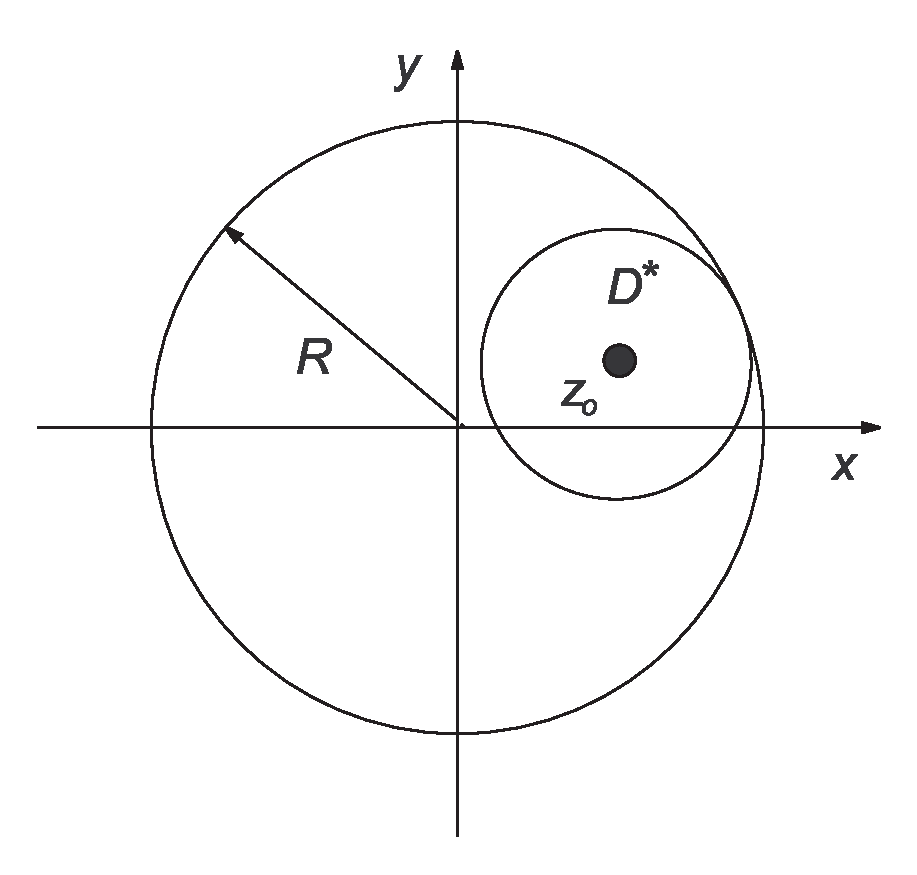
\includegraphics[width=0.4\textwidth]{fig-342.eps}
\caption{Centros diferentes}
\label{fig-342}
\end{figure}

Para estes valores de $z$ podemos, ordenar a s\'{e}rie no \'{u}ltimo
membro de \eqref{funre136:5} em fun\c{c}\~{a}o das pot\^{e}ncias de $Z =z -
z_o$, sem alterar sua soma. Desta maneira obtemos uma
representa\c{c}\~{a}o da forma
\begin{equation}\label{funre136:7}
  f(z)=\sum_{n\geq 0}a_n(z-z_o)^n
\end{equation}
v\'{a}lida (no m\'{\i}nimo) no disco
\begin{equation*}
  |z-z_o|<R-|z_o|.
\end{equation*}

Veremos mais tarde que, em geral, o raio de converg\^{e}ncia de
\eqref{funre136:7} ser\'{a} maior que $R- |z_o|$, de modo que
\eqref{funre136:7} fornece um \textit{prolongamento (continua\c{c}\~{a}o)}
da fun\c{c}\~{a}o $f$ em \eqref{funre136:1} para pontos fora do disco $|z|
< R$.

Este processo de prolongar uma fun\c{c}\~{a}o, dada inicialmente por uma
s\'{e}rie de pot\^{e}ncias v\'{a}lida em uma regi\~{a}o de converg\^{e}ncia $|z| < R$,
al\'{e}m desta regi\~{a}o \'{e} chamado prolongamento anal\'{\i}tico.

Pelo c\'{a}lculo direto segue-se que os coeficientes $a_n$ podem ser
representados em fun\c{c}\~{a}o dos coeficientes $a_n$, da representa\c{c}\~{a}o
original \eqref{funre136:1} sob a forma
\begin{equation}\label{funre136:8}
  a_n=\sum_{m\geq 0}{m+n\choose n }c_{m+n}b^m,\quad \text{ onde }\quad {m+n\choose n}=
  \frac{(m+n)!}{n!m!}
\end{equation}

A aplica\c{c}\~{a}o pr\'{a}tica de \eqref{funre136:8} ser\'{a} em geral dif\'{\i}cil.
Veremos ulteriormente, que no caso em que $f$ em
\eqref{funre136:1} \'{e} uma fun\c{c}\~{a}o conhecida, h\'{a} v\'{a}rios outros
m\'{e}todos de determinar os coeficientes da s\'{e}rie correspondente
\eqref{funre136:7}.

%%%%%%
\subsection{S\'{e}ries de Pot\^{e}ncias Representam Fun\c{c}\~{o}es Anal\'{\i}ticas}
%%%%%

Isto ser\'{a} o principal objetivo desta se\c{c}\~{a}o. Ap\'{o}s uma pequena
prepara\c{c}\~{a}o, deduziremos que cada fun\c{c}\~{a}o anal\'{\i}tica pode ser
representada por uma s\'{e}rie de pot\^{e}ncias, chamadas de S\'{e}ries de
Taylor.

\paragraph{Adi\c{c}\~{a}o ou Substra\c{c}\~{a}o de S\'{e}ries.}
A soma ou substra\c{c}\~{a}o de duas s\'{e}ries de pot\^{e}ncias com raios de
converg\^{e}ncia $R_1$ e $R_2$ respectivamente, fornecem uma s\'{e}rie de
pot\^{e}ncias com raio  menor o igual ao m\'{\i}nimo de $R_1$ e $R_2$.

\begin{prova} Consideremos as somas parciais $S_n(z)$ e $T_n(z)$. Somando termo
a termo e utilizando
\begin{equation*}
    \lim_{n\to\infty}\left\{S_n(z)\pm
    T_n(z)\right\}=\lim_{n\to\infty}S_n(z)\pm T_n(z),
\end{equation*}
com isso mostramos o que desejamos.\qed
\end{prova}

\paragraph{Multiplica\c{c}\~{a}o de S\'{e}ries de Pot\^{e}ncias.}
Consideramos duas s\'{e}ries de pot\^{e}ncias,
\begin{equation*}
    f(z)=\sum_{m\ge 0}a_mz^m\qquad g(z)=\sum_{m\ge 0}b_kz^k
\end{equation*}
e entendemos por multiplica\c{c}\~{a}o de s\'{e}ries de pot\^{e}ncias como a
multiplica\c{c}\~{a}o de cada termo da primeira s\'{e}rie com cada termo da
segunda s\'{e}rie, obtendo-se uma uma s\'{e}rie de pot\^{e}ncias em $z$
chamada de \textsc{Produto de Cauchy} das duas s\'{e}ries, e esta
representada por
\begin{equation*}
    f(z)g(z)=\sum_{n\ge 0}c_nz^n,\qquad c_n=\sum_{m+k=n}a_mb_k
\end{equation*}
onde
\begin{equation*}
c_n=\sum_{m+k=n}a_mb_k=a_ob_n+a_1b_{n-1}+\cdots+a_{n-1}b_1+a_nb_o
\end{equation*}

Esta s\'{e}rie converge absolutamente para cada $z$ que se encontra no
disco de converg\^{e}ncia de cada uma das s\'{e}ries dadas.

\paragraph{Deriva\c{c}\~{a}o e Integra\c{c}\~{a}o de S\'{e}ries de Pot\^{e}ncias.}
Examinamos a seguir a deriva\c{c}\~{a}o e a integra\c{c}\~{a}o termo a termo das
s\'{e}ries de pot\^{e}ncias. Derivando a s\'{e}rie $\dst{\sum_{n\geq 0}\,a_nz^n}$ obtemos a s\'{e}rie
\begin{equation}\label{funre136:9}
\sum_{n\geq 1}na_nz^{n-1}=a_1+2c_2z+3c_3z^2+\cdots
\end{equation}
que \'{e} chamada a s\'{e}rie derivada da s\'{e}rie dada.

\begin{theoc}{}{re136:3} 
A s\'{e}rie derivada de uma s\'{e}rie de pot\^{e}ncias possui o mesmo raio de converg\^{e}ncia 
que a s\'{e}rie original.
\end{theoc}

\prova Seja $na_n + a_n^*$. Ent\~{a}o $\sqrt[n]{|a_n^*|}
=\sqrt[n]{n}\sqrt[n]{|a_n|}$. Como $\sqrt[n]{n}$ vai para um
quando $n$ vai ao infinito segue-se que as sucess\~{o}es
$\sqrt[n]{|a_n^*|}$ e $\sqrt[n]{|a_n|}$, simultaneamente,
convergem para um mesmo limite ou ent\~{a}o divergem. Se elas
divergem, elas s\~{a}o ambas n\~{a}o-limitadas ou limitadas, e neste
\'{u}ltimo caso seus pontos de acumula\c{c}\~{a}o m\'{a}ximos s\~{a}o os mesmos. Da\'{\i} e
do Teorema~\ref{thm:re136:2} da \'{u}ltima se\c{c}\~{a}o decorre a validade do
presente teorema. \hfill $\square$

\begin{theoc}{}{re136:4}
A s\'{e}rie de potências,
\begin{equation*}
\sum_{n\geq 0}\frac{a_n}{n+1}z^{n+1}=a_{0}z+\frac{a_1}{2}z^2+\frac{a_2}{3}z^3+\cdots
\end{equation*}
obtida integrando a s\'{e}rie $a_{0} + a_1z + a_2z^2+\cdots$ termo a
termo possui o mesmo raio de converg\^{e}ncia que a s\'{e}rie original.
\end{theoc}

\begin{prova}
A demonstra\c{c}\~{a}o \'{e} semelhante \`{a} do Teorema~\ref{thm:re136:3}.\qed
\end{prova}

\begin{exer} Considere s\'{e}rie de pot\^{e}ncias
\begin{equation*}
  \sum_{n\geq 1}(n+1)\,z^{n}
\end{equation*}
encontre seu raio de converg\^{e}ncia.
\end{exer}

\begin{solo}
 Para encontrar o raio de converg\^{e}ncia, integramos termo a termo
 e obtemos a s\'{e}rie geom\'{e}trica $\sum_{}\,z^{n+1}$ com raio $R = 1$. \hfill \(\lozenge\)
\end{solo}

As s\'{e}ries de pot\^{e}ncias representam fun\c{c}\~{o}es anal\'{\i}ticas. Mais precisamente.

\begin{theoc}{}{re136:5} 
Uma s\'{e}rie de pot\^{e}ncias com raio de converg\^{e}ncia n\~{a}o-nulo
$R$, representa uma fun\c{c}\~{a}o anal\'{\i}tica em todos os pontos no
interior de seu disco de converg\^{e}ncia. As derivadas desta fun\c{c}\~{a}o
s\~{a}o obtidas, derivando a s\'{e}rie original termo a termo; todas as
s\'{e}ries assim obtidas possuem o mesmo raio de converg\^{e}ncia que a
s\'{e}rie original.
\end{theoc}

\begin{prova} Consideramos a representa\c{c}\~{a}o
\begin{equation*}
f(z)=\sum_{n\geq 0}a_nz^{n},
\end{equation*}
supondo que o raio de converg\^{e}ncia $R$ n\~{a}o \'{e} nulo. Ent\~{a}o podemos
representar $f$ sob a forma \eqref{funre136:7}, e do
Teorema~\ref{thm:re136:1} segue-se que $f$ \'{e} cont\'{\i}nua com centro em
$z_{0}$. Como $z_o$ \'{e} um ponto qualquer no disco $|z|< R$, a fun\c{c}\~{a}o
$f(z)$ \'{e} cont\'{\i}nua em todo o disco. De \eqref{funre136:7} obtemos
$f(z_{0})=a_{0}$ e, portanto,
\begin{equation*}
  \frac{f(z)- f(z_{0})}{z-z_{0}}=a_1 + a_2(z - z_{0}) + a_3(z - z_{0})^2 +
  \cdots
\end{equation*}

De acordo com o Teorema~\ref{thm:re136:1}, a fun\c{c}\~{a}o representada pela
s\'{e}rie de pot\^{e}ncias no segundo membro \'{e} cont\'{\i}nua em $z_o$. Assim,
de acordo com \eqref{funre136:8},
\begin{align}
  f'(z_{0})=\lim_{z\to z_{0}}\frac{f(z)-f(z_{0})}{z-z_{0}} =a_1&=\sum_{m\geq 0}(m+1)a_{m+1}z_{0}^{m}
  \nonumber\\[2ex]
   &=\sum_{k\geq 1}ka_kz_o^{k-1}\label{funre136:10}
\end{align}

Isto mostra que a primeira derivada de $f$ existe em um ponto $z = z_{0}$ do disco $|z|<R$, e pode ser obtida derivando 
a s\'{e}rie original termo a termo; de fato, a s\'{e}rie no \'{u}ltimo membro possui
raio de converg\^{e}ncia $R$, como foi demonstrado no
Teorema~\ref{thm:re136:3}.  Assim $f$ \'{e} anal\'{\i}tica no disco $|z|< R$ e
a demonstra\c{c}\~{a}o fica completa. \qed
\end{prova}

\begin{exer} Considere s\'{e}rie de pot\^{e}ncias
\begin{equation*}
\sum_{n\geq 2}\binom{n}{2}z^{n}=z^2+3z^3+6z^4+10z^5+\cdots
\end{equation*}
encontre seu raio de converg\^{e}ncia.
\end{exer}

\solo
 Para encontrar o raio de converg\^{e}ncia, derivamos duas vezes termo a termo
 a s\'{e}rie geom\'{e}trica $\sum_{}z^{n+1}$ com raio $R = 1$ e multiplicamos o resultado pelo
fator $z^2/2$ para obter a s\'{e}rie dada, logo o raio procurado \'{e}
$R=1$.\hfill \(\lozenge\)

Como a derivada da  fun\c{c}\~{a}o $f$ \'{e}
\begin{equation*}
  f'(z)= \sum_{n\,=\, 1}^{\infty}\, na_nz^{n-1}
\end{equation*}
e \'{e} representada por uma s\'{e}rie de pot\^{e}ncias, podemos aplicar o
Teorema~\ref{thm:re136:5} a $f'$, concluir que $f''$ existe no disco
$|z|<R$, e
\begin{equation*}
  f''(z)=\sum_{n\geq 2}n(n-1)\,a_{n}z^{n-2}
\end{equation*}

Mais geralmente, a derivada de ordem $m$, $f^{(m)}$, de $f$ existe
no disco e
\begin{equation}\label{funre136:11}
f^{(m)}(z)=\sum_{n\geq m} n(n - 1)\cdots(n - m + 1)a_nz^{n-m}.
\end{equation}

Isto significa que $f$ possui derivadas de todas as ordens no
disco. Veremos mais tarde  que toda fun\c{c}\~{a}o anal\'{\i}tica possui
derivadas de todas as ordens e, al\'{e}m disso, pode ser representada
por uma s\'{e}rie de pot\^{e}ncias.

%%%%%%%%%
\section*{Exercícios Propostos} 
%%%%%%%%%
Resolver os seguintes exerc\'{\i}cios sobre s\'{e}ries de fun\c{c}\~{o}es,
\begin{enumerate}[label=\rm{(\arabic*)},ref=\rm{(\arabic*)}]
\item Utilizando o Teorema~\ref{thm:re136:2}, provar que se $f(z)$ em \eqref{funre136:1} for uma
fun\c{c}\~{a}o \'{\i}mpar, ent\~{a}o $a_n =0$ para $n=0,2,4,\ldots$. Dar exemplos.
\item Mostrar que se $f(z)$ em \eqref{funre136:1} for par, ent\~{a}o $a_n = 0$ para $n = 1,
3, 5,\ldots$.
\item Mostrar que $\dst{f(z)=\sum_{n\geq 0}\frac{z^n}{n!}}$ n\~{a}o \'{e} nem par nem \'{\i}mpar.
\item  Utilizando a s\'{e}rie geom\'{e}trica, verificar as afirma\c{c}\~{o}es dos Teoremas~\ref{thm:re136:3}
e \ref{thm:re136:4}.
\item Verificar os Teoremas~\ref{thm:re136:3} e \ref{thm:re136:4} para a
s\'{e}rie$\dst{f(z)=\sum_{n\geq 0}\frac{z^n}{n!}}$.
\item Empregando a s\'{e}rie geom\'{e}trica e os Teoremas~\ref{thm:re136:3} e \ref{thm:re136:4}, determinar os
raios de converg\^{e}ncia das seguintes s\'{e}ries
\begin{tasks}[label=\rm{(\alph*)},item-indent=4em,label-width=4ex,ref=\rm{(\alph*)}](2)
\task  \(\dst \sum_{n\geq 0}\,n(z-j)^{n}\quad   R: \)
\task  \(\dst \sum_{n\geq k}{n\choose k}\,z^{n}\quad  R:\)
\task  \(\dst \sum_{n\geq k}{n\choose k}\left(\dfrac{z}{3}\right)^{n}\quad  R: \)
\task  \(\dst \sum_{n\geq 1}\frac{(-1)^n}{n}(z+1)^{n}\quad  R:\)
\task  \(\dst \sum_{n\geq 1}\frac{z^n}{2^n n(n-1)}\quad  R: \)
\task  \(\dst \sum_{n\geq 1}\frac{(z-2i)^n}{3^n n}\quad  R:\)
\end{tasks}
\item Utilizando o Teorema~\ref{thm:re136:5}, demonstrar as seguintes proposi\c{c}\~{o}es,
\begin{tasks}[label=\rm{(\alph*)},item-indent=4em,label-width=4ex,ref=\rm{(\alph*)}](1)
\task \(\dst{f(z)=\sum_{n\geq 0}\frac{z^n}{n!}}\quad \textrm{ satisfaz a }\quad  f'(z)-f(z)=0\)
\task \(\dst{f(z)=\sum_{n\geq 0}\frac{(-1)^n}{(2n)!}z^{2n}} \quad \textrm{satisfaz a} \quad  f''(z)+f(z)=0\)
\task \(\dst{f(z)=\sum_{n\geq 0}\frac{(-1)^n}{(2n+1)!}z^{2n+1}}\quad  \textrm{ satisfaz a } \quad  f''(z)+f(z)=0.\)
\end{tasks}
\end{enumerate}

%%%%%
\section{S\'{e}rie de Taylor}
%%%%
Na \'{u}ltima se\c{c}\~{a}o vimos que s\'{e}ries de pot\^{e}ncias com raio de converg\^{e}ncia n\~{a}o-nulo representam fun\c{c}\~{o}es anal\'{\i}ticas. Veremos agora que toda fun\c{c}\~{a}o anal\'{\i}tica pode ser representada por uma s\'{e}rie de pot\^{e}ncias. Estas representa\c{c}\~{o}es s\~{a}o chamadas s\'{e}ries de Taylor e s\~{a}o semelhantes \`{a}s s\'{e}ries de Taylor familiares das fun\c{c}\~{o}es reais. Na verdade, substituindo a vari\'{a}vel real nas s\'{e}ries reais por uma vari\'{a}vel complexa podemos prolongar fun\c{c}\~{o}es reais de maneira anal\'{\i}tica dentro do dom\'{\i}nio complexo.


O desenvolvimento familiar em s\'{e}rie de Taylor constitui uma ferramenta eficaz no c\'{a}lculo real e em suas aplica\c{c}\~{o}es. Veremos que na an\'{a}lise complexa o desenvolvimento de Taylor, que \'{e} uma generaliza\c{c}\~{a}o do desenvolvimento acima mencionado, \'{e} ainda mais importante.

Consideramos uma fun\c{c}\~{a}o $f$, que \'{e} anal\'{\i}tica em uma vizinhan\c{c}a de um ponto $z$. Seja $\mathcal{C}$  uma circunfer\^{e}ncia  nesta vizinhan\c{c}a e possui o centro $z$. Podemos ent\~{a}o aplicar a f\'{o}rmula integral de Cauchy,
\begin{equation}\label{tay141:1}
\oint_{\mathcal{C}}\frac{f(w)}{w-z}dw=(2\pi j)f(z)
\end{equation}
onde $z$ \'{e} um ponto fixo arbitr\'{a}rio no interior de $\mathcal{C}$ e
$w$ \'{e} a vari\'{a}vel complexa de integra\c{c}\~{a}o. Temos,
\begin{equation}\label{tay141:2}
 \frac{1}{w - z}=\frac{1}{w - a - (z- a)}= \frac{1}{(w - a)( 1 - \frac{z - a}{w -
 a})}
\end{equation}

Notamos que como $w$ est\'{a} sobre $ \mathcal{C}$ enquanto $z$ est\'{a}
no interior de $ \mathcal{C}$,
\begin{equation}\label{tay141:3}
 \left|\frac{z - a}{w-a}\right| < 1
\end{equation}

Da progress\~{a}o geom\'{e}trica
\begin{equation*}
  1 + q + q^2 +\cdots+ q^n=\frac{1-q^{n+1}}{1- q}=\frac{1}{1- q}-\frac{q^{n+1}}{1- q},\qquad q\neq 1
\end{equation*}
obtemos a rela\c{c}\~{a}o
\begin{equation*}
\frac{1}{1-q}=1 +q +\cdots + q^n + \frac{q^{n+1}} {1- q}
\end{equation*}

Fazendo $q =(z - a)/(w- a)$ segue-se que

\begin{align*}
\frac{1}{1-[(z-a)/(w-a)]} = 1 &+ \frac{z - a}{w-a} +
\left(\frac{z- a}{w-a}\right)^2 +\cdots\\[2ex]
&\cdots+ \left(\frac{z- a}{w - a}\right)^n+\frac{[(z - a)/(w -
a)]^{n+1}}{(w - z)/(w - a)}
\end{align*}

Substitu\'{\i}mos esta express\~{a}o em \eqref{tay141:2}, e ent\~{a}o
\eqref{tay141:2} em \eqref{tay141:1}. Como $z$ e $a$ s\~{a}o
constantes, podemos retirar do sinal de integral as pot\^{e}ncias de
$(z - a)$, e \eqref{tay141:1} passa a apresentar a forma
\begin{align}\label{tay141:4}
  f(z)&=\frac{1}{2\pi j}\oint_{\mathcal{C}}\frac{f(w)}{w-a}dw+
  \frac{z-a}{2\pi j}\oint_{\mathcal{C}}\frac{f(w)}{(w-a)^2}dw+\cdots \nonumber\\[2ex]
   &\quad\cdots + \frac{(z-a)^n}{2\pi j}\oint_{\mathcal{C}}\frac{f(w)}{(w-a)^{n+1}}dw+R_n(z)
\end{align}
onde o \'{u}ltimo termo \'{e} dado pela f\'{o}rmula
\begin{equation}\label{tay141:5}
R_n(z)=  \frac{(z- a)^{n+1}}{ 2\pi
j}\oint_{\mathcal{C}}\frac{f(w)}{(w-a)^{n+1}(w-z)}dw.
\end{equation}

Empregando a derivada geral,
\begin{equation*}
  f^{(n)}(a)=\frac{n!}{2\pi
  ij}\oint_{\mathcal{C}}\frac{f(w)}{(w-a)^{n+1}}dw,\qquad
  n=1,2,3,\ldots
\end{equation*}
podemos escrever \'{e}ste desenvolvimento sob a forma
\begin{align}\label{tay141:6}
f(z)= f(a)&+ \frac{(z-a)}{1!} f'(a)+\frac{(z - a)^2}{2!}f''(a)+\cdots\nonumber\\[2ex]
   &\cdots+ \frac{(z - a)^n}{n!} f^{(n)}(a) + R_n(z).
\end{align}

Esta representa\c{c}\~{a}o constitui a \textsc{F\'{o}rmula de Taylor}.
$R_n(z)$ \'{e} chamado o resto.

Como a fun\c{c}\~{a}o anal\'{\i}tica $f$ possui derivadas de todas as ordens,
podemos tomar $n$ em \eqref{tay141:6} arbitrariamente grande.

Fazendo $n$ se aproximar do infinito, obtemos de \eqref{tay141:6}
a s\'{e}rie de pot\^{e}ncias
\begin{equation}\label{tay141:7}
f(z)=\sum_{m\geq 0}\frac{f^{(m)}(a)}{m!}(z - a)^m.
\end{equation}

Esta s\'{e}rie \'{e} a chamada \textsc{S\'{e}rie de Taylor} de $f$ com centro
em $a$. O caso particular em que $a = 0$ constitui a chamada
\textsc{s\'{e}rie de Maclaurin} de $f$.

Evidentemente, a s\'{e}rie \eqref{tay141:7} converge e representa $f$
se, e somente, se,
\begin{equation}\label{tay141:8}
\lim_{n\to\infty} R_n(z) = 0.
\end{equation}

Para demonstrar \eqref{tay141:8}, consideramos \eqref{tay141:5}.
Como $w$ se encontra sobre $ \mathcal{C}$ enquanto $z$ est\'{a} no
interior de $ \mathcal{C}$, temos $|w - z|>0$. Como $f$ \'{e}
anal\'{\i}tica no interior de $ \mathcal{C}$ e sobre $\mathcal{C}$,
segue-se que o valor absoluto de $f(w)/(w-z)$ \'{e} limitado, digamos
\begin{equation*}
\left|\frac{f(w)}{w - z}\right|<T
\end{equation*}
para todo $w$ sobre $\mathcal{C}$. Seja $r$ o raio de $
\mathcal{C}$. Ent\~{a}o, $ \mathcal{C}$ possui o comprimento $2\pi r$,
e $|w - a | = r$ para todo $w$ sobre $\mathcal{C}$. Assim,
aplicando a f\'{o}rmula fundamental
\begin{equation*}
\left|\oint_{\mathcal{C}} f(z)dz \right|\leq M\cdot L
\end{equation*}
onde $L$ \'{e} o comprimento da tra\c{c}o da curva $\mathcal{C}$ e $M$ \'{e}
uma constante real tal que $|f(z)|\le M$ em qualquer ponto de
$\mathcal{C}$, a \eqref{tay141:5}, obtemos
\begin{align*}
|R_n| &= \frac{|z -a|^{n+1}}{2\pi}\left|\oint_{\mathcal{C}}
\frac{f(w)}{(w -a)^{n+1}(w-z)}dw\right|\\[2ex]
  &<\frac{|z -a|^{n+1}}{2\pi}T\frac{1}{r^{n+1}}2\pi r=T\,r\left|
  \frac{z-a}{r}\right|^{n+1}
\end{align*}

Observamos que $|z-a|<r$ para $z$ dentro ds circunf\^{e}rencia
$\mathcal{C}$, assim $|z-a|/r<1$. Fazendo $n$ se aproximar do
infinito,  a express\~{a}o \`{a} direita se aproxima de zero. Isto
demonstra \eqref{tay141:8} para todo $z$ no interior de $
\mathcal{C}$. Como, pelo Teorema~\ref{thm:re136:2}, a representa\c{c}\~{a}o de
$f$ sob a forma \eqref{tay141:7} \'{e} \'{u}nica, no sentido de que
\eqref{tay141:7} \'{e} a \'{u}nica s\'{e}rie de pot\^{e}ncias com centro em $a$,
que representa a fun\c{c}\~{a}o dada $f$, podemos resumir o resultado como
segue.

\begin{theoc}{Teorema de Taylor}{} Seja $f$ anal\'{\i}tica em um dom\'{\i}nio $\Om$ e seja
$z=a$ um ponto qualquer em $\Om$. Existe, ent\~{a}o, unicamente uma
s\'{e}rie de pot\^{e}ncias com centro em $a$ que representa $f$; esta
s\'{e}rie \'{e} da forma
\begin{equation}\label{tay141:9}
f(z)=\sum_{n\geq 0}b_n(z - a)^n,\quad \text{onde} \quad
b_n=\frac{1}{n!}f^{(n)}(a),\quad n=0,1,\ldots
\end{equation}

Esta representa\c{c}\~{a}o \'{e} v\'{a}lida no disco aberto m\'{a}ximo com centro $a$,
contido em $\Om$. O resto $R_n(z)$ de \eqref{tay141:9} pode ser
representado sob a forma \eqref{tay141:5}. Os coeficientes
satisfazem, \`{a} desigualdade
\begin{equation}\label{tay141:10}
|b_n|\le \frac{M}{r^n}
\end{equation}
onde $M$ \'{e} o m\'{a}ximo de $|f(z)|$  sobre o circunfer\^{e}ncia $|z - a|=
r$.
\end{theoc}

A rela\c{c}\~{a}o \eqref{tay141:10} decorre da desigualdade
\begin{equation*}
  |f^{(n)}(z)|\le \frac{n!M}{r^n}
\end{equation*}
chamada de Cauchy.

Em termos pr\'{a}ticos, \eqref{tay141:8} significa que para todo $z$
para o qual \eqref{tay141:9} converge, a soma parcial de ordem $n$
de \eqref{tay141:9} se aproxima de $f$ com qualquer precis\~{a}o
estabelecida; temos unicamente que escolher $n$ suficientemente
grande.

De acordo com o Teorema de Taylor vemos que o raio de converg\^{e}ncia
de \eqref{tay141:9} \'{e} no m\'{\i}nimo igual \`{a} menor dist\^{a}ncia de $a$ ao
contorno de $\Om$. Ele pode ser maior, mas ent\~{a}o a s\'{e}rie pode n\~{a}o
mais representar $f$ em todos os pontos de $\Om$ que se encontram
no interior do disco de converg\^{e}ncia.

\paragraph{Compara\c{c}\~{a}o com Fun\c{c}\~{o}es de Vari\'{a}vel Real.} Uma
propriedade surpreendente das fun\c{c}\~{o}es anal\'{\i}ticas complexas,
consiste em que elas possuem derivadas, de todas as ordens; outra,
que acabamos de expor, consiste em que elas podem ser sempre
representadas por s\'{e}ries de pot\^{e}ncias da forma \eqref{tay141:9}.
Esta propriedade em geral n\~{a}o \'{e} verdadeira para fun\c{c}\~{o}es reais; h\'{a}
fun\c{c}\~{o}es reais que possuem derivadas de todas as ordens mas n\~{a}o
podem ser representadas por s\'{e}ries de pot\^{e}ncias. Por exemplo a
seguinte fun\c{c}\~{a}o
\begin{equation*}
    f(x)=\left\{%
\begin{array}{ll}
    e^{-1/x^2} & \hbox{ se }\quad x\neq 0 \\[2ex]
    0 & \hbox{ se }\quad x=0 
\end{array}%
\right.
\end{equation*}
esta fun\c{c}\~{a}o n\~{a}o pode ser representada por uma s\'{e}rie de Taylor ao
redor de $z=0$ pois todas a sus derivadas s\~{a}o nulas no ponto
$z=0$.

A rela\c{c}\~{a}o entre o presente estudo e o assunto da se\c{c}\~{a}o anterior
sobre s\'{e}ries de pot\^{e}ncias, pode ser estabelecida pelo seguinte
teorema:

\begin{theoc}{}{ta141:2} 
Toda s\'{e}rie de pot\^{e}ncia com um raio de converg\^{e}ncia n\~{a}o
nulo \'{e} a s\'{e}rie de Taylor da fun\c{c}\~{a}o representada por esta s\'{e}rie.
\end{theoc}

\begin{prova}
Seja a s\'{e}rie de pot\^{e}ncias
\begin{equation*}
  \sum_{n\geq 0}b_n(z - a)^n
\end{equation*}
com um raio de converg\^{e}ncia n\~{a}o nulo $R$. Ent\~{a}o ela representa uma
certa fun\c{c}\~{a}o anal\'{\i}tica $f$ no disco $| z - a | < R$, isto \'{e},
\begin{equation*}
f(z) = b_o + b_1(z -a) + b_2(z - a)^2 +\cdots
\end{equation*}

Do Teorema~\ref{thm:re136:5} segue-se que
\begin{equation*}
  f'(z) = b_1 + 2b_2(z - a) +\cdots
\end{equation*}
e mais geralmente
\begin{equation*}
f^{(n)}(z) = n!\, b_n + (n + 1)\cdot n \cdots 3\cdot2\cdot1\,
b_{n+1}(z - a) +\cdots;
\end{equation*}
todas estas s\'{e}ries convergem no disco $| z - a | < R$. Fazendo $z
= a$ obtemos as seguintes representa\c{c}\~{o}es para os coeficientes da
s\'{e}rie de pot\^{e}ncias:
\begin{equation*}
f(a) = b_o,\quad f'(a) = b_1,\quad\ldots,\quad f^{(n)}(a) = n!
\,b_n,\ldots
\end{equation*}

Estas f\'{o}rmulas s\~{a}o id\^{e}nticas \`{a}s do teorema de Taylor, ent\~{a}o a
demonstra\c{c}\~{a}o est\'{a} completa. \qed
\end{prova}

A f\'{o}rmula da intergral de Cauchy ajuda para expressar os
coeficientes da S\'{e}rie de Taylor
\begin{equation*}
    b_n=\frac{f^{(n)}(a)}{n!}=\frac{1}{2\pi
    j}\oint_{\mathcal{C}}\frac{f(z)}{(z-a)^{n+1}}dz
\end{equation*}
onde se integra no sentido anti-hor\'{a}rio sobre a curva simples e
fechada $\mathcal{C}$, que contem em seu interior o ponto $z=a$.

O ponto em que uma fun\c{c}\~{a}o $f$ deixa de ser anal\'{\i}tica \'{e} chamado um
\textbf{ponto singular} de $f$; podemos tamb\'{e}m dizer que $f$
possui uma singularidade em tal ponto. Mais precisamente: um ponto
$z =z_o$ \'{e} chamado um \textbf{ponto singular} de $f$, se $f$ n\~{a}o
for deriv\'{a}vel em $z_o$ mas, qualquer vizinhan\c{c}a de $z_o$ cont\'{e}m
pontos em que $f$ \'{e} deriv\'{a}vel.

Empregando esse conceito, podemos dizer que existe no m\'{\i}nimo um
ponto singular de $f$ no disco de converg\^{e}ncia isto \'{e}, o raio de
converg\^{e}ncia de \eqref{tay141:9} \'{e}, em geral, igual \`{a} dist\^{a}ncia de
$a$ ao ponto singular de $f$ mais pr\'{o}ximo, mas pode ser maior; por
exemplo, $\ln z$ \'{e} singular ao longo do semi-eixo real negativo, e
a dist\^{a}ncia de $a = - 1 + j$ \`{a}quele eixo \'{e} $1$; entretanto a s\'{e}rie
de Taylor de $\ln z$ com $a = - 1 + j$ tem  raio de converg\^{e}ncia
$\sqrt{2}$.

\subsection{S\'{e}ries de Taylor das Fun\c{c}\~{o}es Elementares}

\begin{exer}[S\'{e}rie Geom\'{e}trica] Seja $f$ uma fun\c{c}\~{a}o complexa de vari\'{a}vel complexa  tal que
$f(z) = 1/(1-z)$. Encontre o seu desenvolvimento de Maclaurin.
\end{exer}

\solo Temos ent\~{a}o $f^{(n)}(z) =n! /(1 - z)^{n+1}$,
$f^{(n)}(z)=n!/(1-z)^{n+1}$. Assim o desenvolvimento de Maclaurin
de $1/(1 - z)$ \'{e} a s\'{e}rie geom\'{e}trica
\begin{equation}\label{elem142:1}
\frac{1}{1-z}=\sum_{n\geq 0}z^n=1 + z + z^2 +\cdots \qquad  |z|
<1,
\end{equation}
logo $f$ \'{e} singular em $z=1$;  este ponto se situa sobre o c\'{\i}rculo
de converg\^{e}ncia. \hfill \(\lozenge\)


\begin{exer}[Fun\c{c}\~{a}o Exponencial]
Considere a fun\c{c}\~{a}o exponencial $e^z$. Analizar suas propriedades.
\end{exer}

\solo  A fun\c{c}\~{a}o exponencial $e^z$
 \'{e} anal\'{\i}tica para qualquer $z$ e que $(e^z)'=e^z$.
Assim, de acordo com \eqref{tay141:9}, com $a = 0$, obtemos a
s\'{e}rie de Maclaurin
\begin{equation}\label{elem142:2}
 e^z =\sum_{n\geq 0}\frac{z^n}{n!}=1+z+z^2+z^3+\cdots
\end{equation}

Esta s\'{e}rie \'{e} tamb\'{e}m obtida quando substitu\'{\i}mos $x$ na s\'{e}rie de
Maclaurin de $e^x$, por $z$. Exprimimos isso afirmando que
prolongamos analiticamente a fun\c{c}\~{a}o exponencial real no dom\'{\i}nio
complexo. \hfill \(\lozenge\)

\bigskip
Provemos a f\'{o}rmula de multiplica\c{c}\~{a}o
\begin{equation}\label{elem142:3}
e^{z_1}e^{z_2}=e^{z_1+z_2}
\end{equation}
empregando \eqref{elem142:2}. Temos
\begin{equation*}
e^{z_1}e^{z_2}=\sum_{k\geq 0}\frac{z_1^k}{k!}\;\sum_{m\geq
0}\frac{z_2^m}{m!}
\end{equation*}

Como ambas as s\'{e}ries convergem absolutamente, podemos
multiplic\'{a}-las termo a termo; a soma dos produtos para os quais $k
+ m= n$ \'{e}
\begin{align*}
\frac{z_1^n}{n!}+\frac{z_1^{n-1}}{(n-1)!}\frac{z_2}{1!}+\cdots+
\frac{z_1}{1!}\frac{z_2^{n-1}}{(n-1)!}+\frac{z_2^n}{n!}&=\\[2ex]
\frac{1}{n!}\left[z_1^n+{n\choose 1}z_1^{n-1}z_2+{n\choose
2}z_1^{n-2}z_2^2+\cdots+z_2^n \right]&=\frac{(z_1+z_2)^n}{n!}
\end{align*}

Ent\~{a}o o produto das duas s\'{e}ries pode ser escrito
\begin{equation*}
\sum_{n\geq 0}\frac{(z_1+z_2)^n}{n!}=e^{z_1+z_2}
\end{equation*}
ficando \eqref{elem142:3} demonstrada.\qed

Al\'{e}m disso, fazendo $z =jy$ em \eqref{elem142:2} e aplicando a
propriedade de adi\c{c}\~{a}o das s\'{e}ries convergentes, obtemos
\begin{equation*}
e^{jy}=\sum_{n\geq 0}\frac{(jy)^n}{n!}=\sum_{k\geq 0}(-1)^k
\frac{y^{2k}}{(2k)!}+j\sum_{k\geq 0}(-1)^k
\frac{y^{2k+1}}{(2k+1)!}
\end{equation*}

Como as s\'{e}ries do segundo membro s\~{a}o os desenvolvimentos de
Maclaurin familiares das fun\c{c}\~{o}es reais $\cos y$ e $\sen y$, este
resultado representa a f\'{o}rmula de Euler
\begin{equation}\label{elem142:4}
e^{jy} = \cos y + j \sen y;
\end{equation}

Multiplicando por $e^x$ e empregando \eqref{elem142:3}, obtemos a
f\'{o}rmula,
\begin{equation*}
e^z=e^x(\cos y +j\sen y)
\end{equation*}
que foi empregada para definir $e^z$. A presente exposi\c{c}\~{a}o mostra
que \'{e} poss\'{\i}vel tamb\'{e}m empregar \eqref{elem142:2} para definir
$e^z$ e deduzir de \eqref{elem142:2} todas as f\'{o}rmulas obtidas nas
se\c{c}\~{o}es anteriores. \qed

\begin{exer}[Fun\c{c}\~{o}es Trigonom\'{e}tricas e Hiperb\'{o}licas]
Escrever as f\'{o}rmulas das fun\c{c}\~{o}es trigom\'{e}tricas e hiperb\'{o}licas em
s\'{e}ries de pot\^{e}ncias.
\end{exer}

\solo  Substituindo o desenvolvimento da exponencial \eqref{elem142:2} nas defini\c{c}\~{o}es de $\sen
z$ e $\cos z$ , obtemos
\begin{align}\label{elem142:5}
  \cos(z) & = \sum_{n\geq 0}(-1)^n\frac{z^{2n}}{(2n)!}=1-\frac{z^2}{2!}+\frac{z^4}{4!}+\cdots\\[2ex]
  \sen(z) &= \sum_{n\geq 0}(-1)^n\frac{z^{2n+1}}{(2n+1)!}=z-\frac{z^3}{3!}+\frac{z^5}{5!}+\cdots
\end{align}

Quando $z = x$ estas s\'{e}ries se transformam nas s\'{e}ries familiares
das fun\c{c}\~{o}es reais $\cos x$ e $\sen x$. Semelhantemente,
substituindo \eqref{elem142:2} em nas defini\c{c}\~{o}es de $\senh z$ e
$\cosh z$ obtemos
\begin{align}\label{elem142:6}
  \cosh(z) &=\sum_{n\geq 0}\frac{z^{2n}}{(2n)!}=1+\frac{z^2}{2!}+\frac{z^4}{4!}+\cdots \\[2ex]
  \senh(z) &=\sum_{n\geq
  0}\frac{z^{2n+1}}{(2n+1)!}=z+\frac{z^3}{3!}+\frac{z^5}{5!}+\cdots
\end{align}

Obtendo assim o que desejavamos. \hfill \(\lozenge\)

\begin{exer}[Logaritmo]
Escrever  a fun\c{c}\~{a}o complexa,  $\dst{\ln\left(\frac{1 +
z}{1-z}\right)}$ em s\'{e}ries de pot\^{e}ncias, utilizando propriedades.
\end{exer}

\solo Pelo Teorema de Taylor, equa\c{c}\~{a}o \eqref{tay141:9} decorre que
\begin{equation}\label{elem142:7}
\ln(1 + z) = z - \frac{z^2}{2} + \frac{z^3 }{3}- \cdots,\qquad
|z|<1.
\end{equation}

Substituindo $z$ por $-z$ e multiplicando ambos os lados por $-
1$, obtemos
\begin{equation}\label{elem142:8}
-\ln(1-z) = \ln \frac{1}{1-z} = z + \frac{z^2}{2} + \frac{z^3}{3}
+\cdots \qquad | z |<1.
\end{equation}

Adicionando ambas as s\'{e}ries obtemos
\begin{equation}\label{elem142:9}
\ln \left(\frac{1 + z}{1-z}\right) = 2
\left[z+\frac{z^3}{3}+\frac{z^5}{5}+\cdots \right]\qquad |z|<1,
\end{equation}
obtemos o que desejamos.\hfill \(\lozenge\)

%%%%%%%
\section*{Exerc\'{\i}cios Propostos} 
%%%%%%%
Resolva os seguintes exerc\'{\i}cios sobre s\'{e}ries de po\^{e}ncias complexas.
\begin{enumerate}[label=\rm{(\arabic*)},ref=\rm{(\arabic*)}]
\item Deduzir as s\'{e}ries de Taylor, em torno do ponto $z = a$, das
fun\c{c}\~{o}es seguintes, e determinar o raio de converg\^{e}ncia.
\begin{tasks}[label=\rm{(\alph*)},item-indent=3em,label-width=4ex,ref=\rm{(\alph*)}](2)
\task \(\cos(2z), \quad   a = 0 \)
\task \(\sen(z^2),\quad a = 0\)
\task \(e^{-z},\quad  a = 0 \)
\task \(e^z,\quad a = 1\)
\task \(e^z,\quad a= \pi i\)
\task \(\sen(z),\quad  a= \pi/2\)
\task \(\cos(z),\quad  a = - \pi/4\)
\task  \(1/(1-z),\quad   a =-1\)
\task \(1/z,\quad   a = 1\)
\task \(1/(1 - z),\quad   a = i\)
\task \(\cos^2(z),\quad   a = 0\)
\task \(\sen^2(z),\quad   a =0\)
\end{tasks}
\item Determinar os tr\^{e}s primeiros termos das s\'{e}ries de Maclaurin
das fun\c{c}\~{o}es seguintes.
\begin{tasks}[label=\rm{(\alph*)},item-indent=3em,label-width=4ex,ref=\rm{(\alph*)}](2)
\task \(\tan(z)\)
\task \(\tan(2z)\)
\task \(e^z \sen(z)\)
\task \(z \cot(z)\)
\end{tasks}
\item Determinar as s\'{e}ries de Maclaurin integrando termo a termo as
dos integrandos.
\begin{tasks}[label=\rm{(\alph*)},item-indent=3em,label-width=4ex,ref=\rm{(\alph*)}](2)
\task  \(\dst{\int_0^z e^t\, dt}\)
\task \(\dst{\int_0^z \cos(t)\, dt}\)
\task \(\dst{\int_0^z \sen(t)\, dt}\)
\task \(\dst{\int_0^z \frac{e^t-1}{t}\, dt}\)
\task \(\dst{\int_0^z e^{t^2}\,dt}\)
\task \(\dst{\int_0^z \frac{\sen t}{t}\, dt}\)
\task \(\dst{\int_0^z \cos(t^2)\, dt}\)
\task \(\dst{\int_0^z \sen(t^2)\, dt}\)
\end{tasks}
\end{enumerate}

%%%%%
\section{M\'{e}todos para Obten\c{c}\~{a}o de S\'{e}ries de Pot\^{e}ncias}
%%%%
Na maioria dos casos pr\'{a}ticos, a determina\c{c}\~{a}o dos coeficientes de
uma s\'{e}rie de Taylor por meio da f\'{o}rmula do teorema de Taylor \'{e}
complicada, ou consome muito tempo. Existe um certo n\'{u}mero de
processos pr\'{a}ticos mais simples para atingir tal fim, que podem
ser ilustrados pelos seguintes exemplos. A unicidade das
representa\c{c}\~{o}es assim obtidas decorre do Teorema da Unicidade de
s\'{e}ries de pot\^{e}ncias.

\begin{exer}[Substitui\c{c}\~{a}o]
Determinar a s\'{e}rie de Maclaurin de $f(z)=1/(1 + z^2)$.
\end{exer}

\solo Substituindo $-z^2$ por $z$ em \eqref{elem142:1}, obtemos
\begin{align}\label{pra143:1}
  \frac{1}{1+z^2}=\frac{1}{1-(-z^2)} &= \sum_{n\geq 0}(-z^2)^n=\sum_{n\geq 0}(-1)^nz^{2n}\\[2ex]
  &=1-z^2+z^4-z^6+\cdots,\qquad |z|<1\nonumber
\end{align}

Assim determinamos a s\'{e}rie pedida. \hfill \(\lozenge\)

\begin{exer}[Integra\c{c}\~{a}o] Seja $f(z)= \arctan z$. Escreva sua s\'{e}rie
de pot\^{e}ncias.
\end{exer}

\solo Temos $f'(z)= 1/(1 + z^2)$.

Integrando \eqref{pra143:1} termo a termo e notando que $f(0)= 0$,
encontramos
\begin{equation*}
\arctan z=\sum_{n\geq
0}\frac{(-1)^n}{2n+1}z^{2n+1}=z-\frac{z^3}{3}+\frac{z^5}{5}-+\cdots
\quad |z|<1
\end{equation*}
esta s\'{e}rie representa o valor principal de $w = u + jv = \arctan
z$, definido como o valor para o qual $|u|<\pi/2$. \hfill \(\lozenge\)


\begin{exer}[S\'{e}rie Geom\'{e}trica] Desenvolver
$1/(c - bz)$ em pot\^{e}ncias de $z - a$ onde $c - ab \neq 0$ e $b
\neq 0$.
\end{exer}

\solo Evidentemente
\begin{equation*}
\frac{1}{c - bz} = \frac{1}{c-ab-b(z - a)} = \frac{1}{(c -
ab)\left[1- \frac{b(z - a)}{c - ab}\right]}
\end{equation*}

\`{A} \'{u}ltima express\~{a}o aplicamos \eqref{elem142:1} com $z$ substitu\'{\i}do
por $b(z - a)/(c - ab)$, obtendo
\begin{equation*}
\frac{1}{c- bz}=\frac{1}{c-ab}\sum_{n\geq
0}\left[\frac{b(z-a)}{(c-ab)}\right]^n=\sum_{n\geq
0}\frac{b^n}{(c-ab)^{n+1}}(z-a)^n
\end{equation*}

Escrevendo a \'{u}ltima s\'{e}rie por extenso
\begin{equation*}
\frac{1}{c- bz}= \frac{1}{c - ab}+ \frac{b}{(c - ab)^2}(z - a)+
 \frac{b^2}{(c-ab)^3}(z - a)^2+\cdots
\end{equation*}

Esta s\'{e}rie converge para
\begin{equation*}
\left|\frac{b(z - a)}{c-ab}\right| < 1\quad\text{isto \'{e}},\quad |z
- a| < \left|\frac{c - ab}{b}\right|=\left|\frac{c}{b}-a\right|
\end{equation*}

Obtendo o desenvolvimento desejado. \hfill \(\lozenge\)

\begin{exer}[S\'{e}rie Binomial, Dedu\c{c}\~{a}o por Fra\c{c}\~{o}es Parciais]
Determinar a s\'{e}rie de Taylor da fun\c{c}\~{a}o
\begin{equation*}
f(z)= \frac{2z^2 +9z +5 }{z^3 + z^2 - 8z - 12}
\end{equation*}
com centro em $z = 1$.
\end{exer}

\solo Dada uma fun\c{c}\~{a}o racional, quando o grau do polin\^{o}mio do numerador \'{e} menor que o grau do
polin\^{o}mio do denominador podemos aplicar a t\'{e}cnica de fra\c{c}\~{o}es parciais, caso contr\'{a}rio fazemos uma divis\~{a}o de
polin\^{o}mios at\'{e} obter que o grau do polin\^{o}mio do numerador seja menor que o grau do denominador.

Podemos inicialmente representar a fun\c{c}\~{a}o $f$ como uma soma de fra\c{c}\~{o}es parciais da seguinte maneira,
\begin{equation}\label{troy}
  f(z)=\frac{2z^2 +9z +5 }{z^3 + z^2 - 8z - 12}=\frac{2z^2 +9z +5 }{(z-3)(z^2 +4z +4)}
  =\frac{A}{z-3}+\frac{Bz+C}{z^2+4z+4}
\end{equation}
onde $z=3$ \'{e} raiz do denominador. Devemos encontrar as constantes $A$, $B$ e $C$. A identiadade acima deve ser
v\'{a}lida para quaisquer $z$.

Para calcular o valor de $A$, multiplicamos a identidade acima por $z-3$ para obter
\begin{equation*}
\frac{2z^2 +9z +5 }{z^2 +4z +4}
  =A+\frac{(Bz+C)(z-3)}{z^2+4z+4}
\end{equation*}
e avaliando em $z=3$ encontramos que $A=2$.

Multiplicando a identidade \eqref{troy} acima por $z^2+4z+4$ temos
\begin{equation*}
\frac{2z^2 +9z +5 }{z-3}
  =\frac{A(z^2+4z+4)}{z-3}+Bz+C
\end{equation*}
e avaliando em $z=0$ temos $C=1$.

Finalmente avaliando em $z=4$ na express\~{a}o \eqref{troy}, temos $B=0$. Portanto escrevemos
\begin{equation*}
f(z) = \frac{1}{(z+2)^2} +\frac{2}{z-3}= \frac{1}{[3 + (z - 1)]^2}
-\frac{2}{2- (z - 1)}
\end{equation*}
e em seguida aplicar a s\'{e}rie binomial
\begin{align}\label{pra143:2}
  \frac{1}{(1+z)^m} &=\sum_{n\geq 0}{-m\choose n}z^n  \nonumber\\[2ex]
   & =1-mz+\frac{m(m+1)}{2!}z^2-\frac{m(m+1)(m+2)}{3!}z^3+\cdots
\end{align}
e como a fun\c{c}\~{a}o do primeiro membro \'{e} singular em $z=-1$, a s\'{e}rie
converge no disco $|z| < 1$.

No caso presente obtemos, escrevemos sob a forma
\begin{equation*}
f(z) = \frac{1}{9}\frac{1}{\dst{\left(1 + \frac{z - 1}{3}\right)^2}}-
\frac{1}{\dst{1 - \frac{z - 1}{2}}}.
\end{equation*}

Utilizando a s\'{e}rie do bin\^{o}mio obtemos
\begin{equation*}
f(z)=\frac{1}{9}\sum_{n\geq 0}{-2\choose n}
\left(\frac{z-1}{3}\right)^n - \sum_{n\geq 0}
\left(\frac{z-1}{2}\right)^n
\end{equation*}

Podemos adicionar termo a termo as duas s\'{e}ries do segundo membro.
Como o coeficiente binomial na primeira s\'{e}rie \'{e} igual
\begin{align*}
{-2\choose n}&=\frac{(-2)(-2-1)(-2-2)(-2-3)\cdots(-2-n+1)}{n!}\\[2ex]
&=(-1)^n\frac{(1)(2)(3)(4)(5)\cdots(n+1)}{n!}=(-1)^n\frac{n!(n+1)}{n!}=(- 1)^n(n + 1)
\end{align*}
obtemos
\begin{equation*}
f(z)=\sum_{n\geq
0}\left[\frac{(-1)^n(n+1)}{3^{n+2}}-\frac{1}{2^n}\right](z-1)^n.
\end{equation*}

Escrevendo este resultado por extenso temos
\begin{equation*}
  f(z)= -\frac{8}{9} - \frac{31}{54} (z -1) - \frac{23}{108} (z-
1)^2-\cdots
\end{equation*}

Devemos ressaltar que  $z = 3$ \'{e} o ponto singular de $f$ que se
encontra mais pr\'{o}ximo do centro $z=1$, ent\~{a}o a s\'{e}rie converge, por
propriedade de converg\^{e}ncia, no disco aberto $|z - 1|< 2$.\hfill
\(\lozenge\)


\begin{exer}[Equa\c{c}\~{o}es Diferenciais] Determinar a s\'{e}rie de
Maclaurin da fun\c{c}\~{a}o de vari\'{a}vel complexa, $f(z)=\tan(z)$.
\end{exer}

\solo Derivando temos $f'(z)= \sec^2(z)$, e utilizando a identidade
\begin{equation*}
f'(z) = 1 + f^2(z)\qquad\text{ ent\~{a}o }\qquad  f'(0) = 1.\quad \text{ onde }\quad  f(0)=0.
\end{equation*}

Derivamos sucessivamente a identidade
anterior
\begin{align*}
&f''(z)=2f(z)f'(z), && f''(0)=0, && \\[2ex]
&f'''(z)=2[f'(z)]^2+2f(z)f''(z), && f'''(0)=2,&& \frac{f'''(0)}{3!}=\frac{1}{3},\\[2ex]
&f^{(4)}(z)=6f'(z)f''(z)+2f(z)f'''(z), &&f^{(4)}(0)=0, &&\\[2ex]
&f^{(5)}(z)=6[f''(z)]^2+8f'(z)f'''(z)+2f(z)f^{(4)}(z), &&f^{(5)}(0)=16, &&\frac{f^{(5)}}{5!}=\frac{2}{15},
\end{align*}
de forma an\'{a}loga podemos seguir obtendo os demais coeficientes da
s\'{e}rie. Portanto, obtemos o resultado
\begin{equation}\label{pra143:3}
\tan(z) = \sum_{n\ge 0}\frac{f^{(n)}(0)}{n!}z^n=z + \frac{1}{3}z^3 + \frac{2}{15} z^5 +
\frac{17}{315}z^{17} +\cdots \qquad |z|<\pi/2.
\end{equation}

Obtemos assim o resultado desejado.\hfill \(\lozenge\)

\begin{exer}[Coeficientes a Determinar]
Calcular a s\'{e}rie de Maclaurin de $\tan z$ utilizando o desenvolvimento em s\'{e}ries de
$\sen(z)$ e $\cos(z)$.
\end{exer}

\solo Como $\tan(z)$ \'{e} fun\c{c}\~{a}o \'{\i}mpar, o desenvolvimento desejado ser\'{a} da
forma
\begin{equation*}
\tan(z) = b_1z + b_3z^3 + b_5z^5 +\cdots
\end{equation*}

Utilizando a rela\c{c}\~{a}o $\sen z =\tan z \cos z$, obtemos substituindo os
desenvolvimentos de seno, tangente e cosseno,
\begin{equation*}
  z - \frac{z^3}{3!} + \frac{z^5}{5!}- +\cdots= (b_1z + b_3z^3 + b_5z^5
  +\cdots)\left(1-\frac{z^2}{2!} + \frac{z^4}{4!}- +\cdots
  \right).
\end{equation*}

Como $\tan(z)$ \'{e} anal\'{\i}tica exceto em $z =\pm \pi/2,\pm
3\pi/2,\cdots$ sua s\'{e}rie de Maclaurin converge no disco $|z|
<\pi/2$, e para estes valores de $z$ podemos multiplicar as duas
s\'{e}ries no segundo membro, termo a termo, ordenando a s\'{e}rie
resultante segundo as pot\^{e}ncias crescentes de $z$ segundo o
produto de Cauchy das s\'{e}ries.

De acordo com o teorema de unicidade, Teorema~\ref{thm:re136:2}, o coeficiente de
cada pot\^{e}ncia de $z$ \'{e} o
mesmo em ambas as s\'{e}ries. Assim
\begin{align*}
&1= b_1, && -\frac{1}{3!}=-\frac{b_1}{2!}+ b_3,&& \frac{1}{5!} = \frac{b_1}{4!}- \frac{b_3}{2!}+ b_5
\end{align*}
Portanto, $b_1 = 1$, $b_3=1/3$, $b_5=2/15$,\; \ldots.

Mencionamos que existem tabelas dos chamados n\'{u}meros de Bernoulli
$B_n$ que permitem facilmente o c\'{a}lculo dos coeficientes da s\'{e}rie tangente
\eqref{pra143:3}.

Os n\'{u}meros $\dst{\frac{B_n}{n!}}$ s\~{a}o por defini\c{c}\~{a}o os
coeficientes da s\'{e}rie de Maclaurin
\begin{equation}\label{pra143:4}
\frac{z}{e^z-1} = 1 + B_1z + \frac{B_2}{2!}z^2 +
\frac{B_3}{3!}z^3+\ldots
\end{equation}

Pelo m\'{e}todo dos coeficientes a determinar obtemos
\begin{align}\label{pra143:5}
&B_1=-\frac{1}{2},&&  B_2= \frac{1}{6},&&
B_4=-\frac{1}{30}, &&  B_5=0, && B_6=\frac{1}{42},\ldots
\end{align}

Das defini\c{c}\~{o}es de $\cos(z)$ e $\tan(z)$  segue-se que
\begin{equation*}
  \tan(z) = \frac{2i}{e^{2iz}-1}- \frac{4j}{e^{4jz}-1}-i
\end{equation*}
como o estudante pode verificar. Pelo resultado anterior  e a rela\c{c}\~{a}o \eqref{pra143:4} obtemos
\begin{equation}\label{pra143:6}
\tan(z)= \frac{4\cdot
3}{2!}B_2z+\cdots+(-1)^{n-1}\frac{2^{2n}(2^{2n}-1)}{(2n)!}B_{2n}z^{2n-1}+\cdots
\end{equation}

Portanto obtemos a s\'{e}rie requisitada. \hfill \(\lozenge\)

%%%%
\section*{Exerc\'{\i}cios Propostos} 
%%%%%
Resolver as seguintes quest\~{o}es sobre s\'{e}ries num\'{e}ricas,
\begin{enumerate}[label=\rm{(\arabic*)}]
\item  Determinar as s\'{e}ries de Maclaurin das fun\c{c}\~{o}es seguintes
\begin{tasks}[label=\rm{(\alph*)},item-indent=3em,label-width=4ex,ref=\rm{(\alph*)}](2)
\task  \(\dst{\dfrac{1}{1-z^3}}\)
\task  \(\dst{\dfrac{1}{1+z^3}}\)
\task \(\dst{\dfrac{1}{1-z^6}}\)
\task  \(\dst{\dfrac{1}{(1+z^2)^2}}\)
\task  \(\dst{\sen(z^3)}\)
\task  \(\dst{\cos(z^2)}\)
\task  \(\dst{e^{z^2-z}}\)
\task  \(\dst{e^{z^4}}\)
\task  \(\dst{\dfrac{\sqrt{z}}{2}\int_0^z\frac{\cos t}{\sqrt{t}}dt}\)
\task  \(\dst{\dfrac{\sqrt{z}}{2}\int_0^z\frac{\sen(t)}{\sqrt{t}}dt}\)
\task \(\dst{e^{z^2}\int_0^ze^{-t^2}\,dt}\)
\end{tasks}

\item Desenvolvendo $1/\sqrt{1-z^2}$ e integrando, mostrar que
\begin{equation*}
\arcsen(z) = z + \left(\frac{1}{2}\right) \frac{z^3}{3}+
\left(\frac{1\cdot 3}{2\cdot 4 }\right)\frac{z^5}{5}+
\left(\frac{1\cdot 3\cdot 5}{2\cdot 4\cdot
6}\right)\frac{z^7}{7}+\cdots,\qquad |z|<1.
\end{equation*}
\item  Determinar os primeiros termos das s\'{e}ries de Maclaurin das fun\c{c}\~{o}es seguintes.
\begin{tasks}[label=\rm{(\alph*)},item-indent=3em,label-width=4ex,ref=\rm{(\alph*)}](3)
\task \(\dst{e^{e^z}}\)
\task  \(\dst{\cos \left(\frac{z}{1-z}\right)}\)
\task  \(\dst{e^{1/(1-z)}}\)
\end{tasks}
\item Determinar o desenvolvimento em s\'{e}rie de Taylor da fun\c{c}\~{a}o dada
em torno de $z=a$.
\begin{tasks}[label=\rm{(\alph*)},item-indent=3em,label-width=4ex,ref=\rm{(\alph*)}](2)
\task  \(\dst{\frac{1}{2z-j}},\quad a=-1\)
\task \(\dst{\frac{1}{4-3z}},\quad  a=1+i\)
\task  \(\dst{\frac{1}{1-z}},\quad a=2i\)
\task  \(\dst{\frac{1}{(1+z)^2}},\quad a=-i\)
\task  \(\dst{\frac{1}{(2+3z^3)^2}},\quad a=0 \)
\task  \(\tan(z),\quad a=\pi/4.\)
\end{tasks}
\item \textbf{(N\'{u}meros de Euler)} O desenvolvimento
\begin{equation*}
\sec(z) = E_{0}- \dfrac{E_2}{2!} z^2 + \dfrac{E_4}{4!}z^4 - +\cdots
\end{equation*}
define os n\'{u}meros de Euler $E_{2n}$. Mostrar que $E_{0} = 1$, $E_2=-
1$, $E_4 = 5$, $E_6=-61$.
\end{enumerate}

%%%%
\section{Converg\^{e}ncia Uniforme}
%%%%

Suponhamos que sabemos que uma dada s\'{e}rie converge em uma certa
regi\~{a}o $\Om$; a quest\~{a}o que resta examinar \'{e} se a converg\^{e}ncia \'{e}
suficientemente r\'{a}pida atrav\'{e}s de toda a regi\~{a}o ou se h\'{a} pontos em
cuja proximidade a converg\^{e}ncia se torna lenta. A import\^{a}ncia
pr\'{a}tica desta quest\~{a}o em problemas de c\'{a}lculo num\'{e}rico \'{e} evidente;
veremos entretanto que o aspecto te\'{o}rico da quest\~{a}o \'{e} at\'{e} mais
importante. Para ilustrar a situa\c{c}\~{a}o vamos iniciar com alguns
exemplos.

\begin{exer}\label{ex144:1}
Calcular uma tabela de $e^x$ para $x$ real no intervalo $0\le x
\le 1$.
\end{exer}

\solo Por exemplo, para $x= 0,\; 0,1,\; 0,2,\ldots$ devendo o
valor absoluto do erro de cada valor ser menor que um dado n\'{u}mero
$\vep$, digamos, menor que meia unidade do sexto algarismo
decimal. Podemos empregar uma soma parcial adequada
\begin{equation*}
s_n= 1 +x +\cdots + \frac{x^n}{n!}
\end{equation*}
da s\'{e}rie de Maclaurin. Ent\~{a}o o valor absoluto do erro \'{e} igual a
$|R_n|=|s - s_n|$ onde $s=e^x$ \'{e} a soma da s\'{e}rie, e devemos
escolher $n$ de tal maneira que
\begin{equation*}
|s(x) - s_n(x)| < \vep (= 5\times 10^{-7}).
\end{equation*}

Pela rela\c{c}\~{a}o, $|R_n|\leq |z_{n+1}|/(1-q)$ vemos que quando $x =
1$, para $n=10$, e portanto para qualquer $n > N = 9$, obtemos a
precis\~{a}o desejada. O resto diminui em valor absoluto quando $x\geq
0$ diminui, e portanto,
\begin{equation*}
| s(x) - s_n(x)| < \vep \quad \text{para}\quad  n > N(\vep) (=
9)\quad\text{e qualquer}\qquad x \in \mathbb{R}
\end{equation*}
sob considera\c{c}\~{a}o. Notamos que, naturalmente, $N$ depende de
$\vep$, e se desejarmos valores mais precisos de sorte que $\vep$
seja menor, ent\~{a}o $N$ ser\'{a} maior. \hfill \(\lozenge\)


\begin{exer}\label{ex144:2}
No caso da s\'{e}rie geom\'{e}trica $1 + z + z^2+\cdots$ Qual \'{e} a forma do resto?
\end{exer}

\solo Como a s\'{e}rie geometrica \'{e} convergente em $|z|<1$. O resto \'{e}
\begin{equation*}
R_n(z) = s(z) -
s_n(z)=\sum_{m=n+1}^{\infty}z^m=\frac{z^{n+1}}{1-z}
\end{equation*}

e se torna arbitrariamente grande para $z = x < 1$ real e
suficientemente pr\'{o}xima de um. Assim, sendo fixado um erro m\'{a}ximo
$\vep$, n\~{a}o podemos determinar um $N$ dependende unicamente de
$\vep$, tal que $|R_n(x)| = |s(x) - s_n(x)| < \vep$ para $n > N$ e
qualquer $x$ no intervalo $0 \le x < 1$. \hfill \(\lozenge\)


O resultado do Exemplo~\ref{ex144:2} anterior n\~{a}o \'{e} completamente
inesperado, porque a s\'{e}rie diverge para $z = 1$. Uma situa\c{c}\~{a}o
realmente surpreendente ocorre no caso da s\'{e}rie seguinte.

\begin{exer}\label{ex144:3}
Consideremos a s\'{e}rie
\begin{equation*}
x^2 + \frac{x^2}{1 + x} + \frac{x^2}{(1 + x^2)^2}+\frac{x^2}{(1 +
x^2)^3} +\cdots
\end{equation*}
Mostre que s\'{e}rie possui soma descont\'{\i}nua em $x=0$.
\end{exer}

\solo Empregando a f\'{o}rmula para a soma de uma progress\~{a}o
geom\'{e}trica, o leitor pode verificar prontamente que a soma parcial
de ordem $n$ \'{e}
\begin{equation*}
s_n(x)= 1 + x^2 -  \frac{1}{(1 + x^2)^n}
\end{equation*}

Assim, se $x\neq 0$ a s\'{e}rie possui a soma
\begin{equation*}
s(x)=\lim_{n\to\infty}s_n(x)=1+x^2
\end{equation*}

Se $x = 0$, ent\~{a}o $s_n = 0$ para todo $n$ e, portanto,
\begin{equation*}
s(0) = \lim_{n\to\infty}s_n( 0)=0
\end{equation*}

Isto mostra que a s\'{e}rie converge para todo $x$ (de maneira
absoluta), mas temos o resultado surpreendente de que a soma \'{e}
descont\'{\i}nua (em $x = 0$), se bem que todos os termos da s\'{e}rie
sejam fun\c{c}\~{o}es cont\'{\i}nuas. Al\'{e}m disso, quando $x\neq 0$ o valor
absoluto do resto \'{e}

\begin{equation*}
|R_n(x)| = |s(x) - s_n(x)|=\frac{1}{(1+x^2)^n}
\end{equation*}
e vemos que para um dado $\vep< 1$ n\~{a}o podemos encontrar um $N$
que dependa somente de $\vep$, e tal que $|R_n| < \vep$ para todo
$n> N(\vep)$ e todo $x$ no intervalo $0\le x \le 1$. \hfill
\(\lozenge\)

%%%%%%%%%%%%%
\section*{Converg\^{e}ncia Uniforme} 
%%%%%%
As s\'{e}ries nos exemplos s\~{a}o da
forma
\begin{equation}\label{form144:1}
\sum_{n\geq 0}f_n(z) = f_o(z) + f_1(z) + f_2(z)+\cdots
\end{equation}

Supomos que \eqref{form144:1} seja convergente para todo $z$ em
uma regi\~{a}o $\Om$. Seja $s(z)$ a soma e $s_n(z)$ a soma parcial de
ordem $n$ de \eqref{form144:1}. Sabemos que a converg\^{e}ncia de
\eqref{form144:1} em um ponto $z$ significa que, dado um $\vep >
0$, podemos determinar um $N(\vep, z)$ tal que
\begin{equation*}
|s(z)-s_n(z)| < \vep\qquad\text{para todo}\quad n > N(\vep, z).
\end{equation*}

$N$ depende de $\vep$ e depender\'{a}, em geral, tamb\'{e}m do ponto $z$
escolhido para exame. Casos h\'{a} em que sendo dado um $\vep > 0$
podemos encontrar um n\'{u}mero $N(\vep)$, \textit{independente} de
$z$, tal que
\begin{equation*}
| s(z) - s_n(z)| < \vep\quad \text{para todo}\quad n >N(\vep)\quad
\text{e todo}\quad z \in \Om.
\end{equation*}

A s\'{e}rie ent\~{a}o \'{e} dita \textit{uniformemente convergente} em $\Om$.

A uniformidade da converg\^{e}ncia \'{e} ent\~{a}o uma propriedade que depende
de todo um conjunto de valores de $z$, enquanto a converg\^{e}ncia de
uma s\'{e}rie pode ser considerada para v\'{a}rios valores particulares de
$z$ sem refer\^{e}ncia a outros valores.

A s\'{e}rie no Exemplo~\ref{ex144:1} \'{e} uniformemente convergente no
intervalo $0\le  x\le 1$ (e na realidade em qualquer regi\~{a}o
limitada do plano $\mathbb{C}$), enquanto a s\'{e}rie do
Exemplo~\ref{ex144:3} n\~{a}o \'{e} uniformemente convergente em uma
regi\~{a}o que cont\'{e}m o ponto $0$. Isto mostra que uma s\'{e}rie
absolutamente convergente pode n\~{a}o ser uniformemente convergente.
Reciprocamente, as s\'{e}ries uniformemente convergentes podem n\~{a}o ser
absolutamente convergentes. Este fato \'{e} ilustrado pelo

\begin{exer}\label{ex144:4} A s\'{e}rie de pot\^{e}ncias dada por,
\begin{equation*}
\sum_{n\geq 1}\frac{(-1)^{n-1}}{x^2+n}=
\frac{1}{x^2+1}-\frac{1}{x^2+2}+\frac{1}{x^2+3}-+\cdots,\qquad
x\in \mathbb{R}
\end{equation*}
\'{e} uniformemente convergente para todo $x$ real mas n\~{a}o \'{e}
absolutamente convergente.
\end{exer}

\solo Utilizando o crit\'{e}rio de Leibnitz o resto $R_n$ n\~{a}o excede
seu primeiro termo em m\'{o}dulo, pois temos uma s\'{e}rie alternada cujos
valores absolutos formam uma sequ\^{e}ncia decrescente  com limite
zero. Assim para $\varepsilon>0$ e apara qualquer $x$, temos que
\begin{equation*}
    |R_n(x)|\le \frac{1}{x^2+n+1}<\frac{1}{n}<\varepsilon,\quad
    n>N(\varepsilon)=\frac{1}{\varepsilon}
\end{equation*}
e como $N(\varepsilon)$ n\~{a}o depende de $x$, temos converg\^{e}ncia
uniforme.

Por outro lado a converg\^{e}ncia n\~{a}o \'{e} absoluta, pois
\begin{equation*}
    \left|\frac{(-1)^{n-1}}{x^2+n}\right|=\frac{1}{x^2+n}>\frac{k}{n}
\end{equation*}
para uma constante $k$ escolhida apropriadamente, e o termo
generico da direita na desigaualdade anterior faz parte da s\'{e}rie
num\'{e}rica harm\^{o}nica que \'{e} divergente.\hfill \(\lozenge\)


O Exemplo~\ref{ex144:2} \'{e} t\'{\i}pico das s\'{e}ries de pot\^{e}ncias porque
para tais s\'{e}ries a situa\c{c}\~{a}o \'{e} simples, como mostra o

\begin{teo}\label{orf144:1} Uma s\'{e}rie de pot\^{e}ncias
\begin{equation}\label{form144:2}
 \sum_{n\geq 0}b_n(z - a)^n
\end{equation}
com um raio de converg\^{e}ncia $R$ n\~{a}o nulo, \'{e} uniformemente
convergente em todo disco circular $|z-a|\le  r$ de raio $r < R$.
\end{teo}

\prova Para $|z - a|\le  r$ temos
\begin{align}
  |a_{n+1}(z-a)^{n+1}+\cdots+a_{n+p}(z-a)^{n+p}| & \nonumber \\
   &\le |a_{n+1}|r^{n+1}+\cdots+|a_{n+p}|r^{n+p}\label{form144:3}
\end{align}

Como \eqref{form144:2} converge absolutamente para $z = r$,
segue-se do Teorema de Cauchy para converg\^{e}ncia se s\'{e}ries que,
dado um $\vep
> 0$, podemos encontrar um $N(\vep)$ tal que
\begin{equation*}
|a_{n+1}|r^{n+1}+\cdots+|a_{n+p}|r^{n+p} < \vep\quad \text{
para}\quad n> N(\vep) \; e \; p = 1, 2,\ldots
\end{equation*}

Da\'{\i} e de \eqref{form144:3} inferimos que
\begin{equation*}
|a_{n+1}(z-a)^{n+1}+\cdots+a_{n+p}(z-a)^{n+p}| < \vep
\end{equation*}
para todo $z$ no disco $| z - a| \le r$, todo $n > N(\vep)$ e
qualquer $p = 1, 2,\ldots$. Como $N(\vep)$ \'{e} independente de $z$,
existe a converg\^{e}ncia uniforme, com o que o teorema fica provado.
\hfill $\Box$

Enquanto a soma de um n\'{u}mero finito de fun\c{c}\~{o}es cont\'{\i}nuas \'{e}
cont\'{\i}nua, o Exemplo~\ref{ex144:3}  mostra que a soma de uma s\'{e}rie
infinita de fun\c{c}\~{o}es cont\'{\i}nuas pode ser descont\'{\i}nua, mesmo que a
s\'{e}rie seja absolutamente convergente. Quando, por\'{e}m, a s\'{e}rie
converge de maneira uniforme isto n\~{a}o pode acontecer. De fato, \'{e}
v\'{a}lido o seguinte.

\begin{teo} \label{orf144:2}
Seja a s\'{e}rie de fun\c{c}\~{o}es,
\begin{equation*}
\sum_{m\geq 0}f_m(z)=f_o(z)+f_1(z)+\cdots,
\end{equation*}
uniformemente convergente em uma regi\~{a}o $\Om$ e seja $F(z)$ a sua
soma. Ent\~{a}o, se cada termo $f_n(z)$ for cont\'{\i}nuo em um ponto $z_o$
em $\Om$, a fun\c{c}\~{a}o $F(z)$ \'{e} cont\'{\i}nua em $z_o$.
\end{teo}

\prova Seja $s_n(z)$ a soma parcial de ordem $n$ da s\'{e}rie e
$R_n(z)$ o resto correspondente:
\begin{equation*}
s_n=f_o+f_1+f_2+\cdots+f_n,\qquad R_n=f_{n+1}+f_{n+2}+\cdots
\end{equation*}

Dado $\vep > 0$, podemos determinar um $n = N(\vep)$ tal que
\begin{equation*}
|R_N(z)| < \frac{\vep}{3}\quad \text{ para todo } z \in  \Om,
\end{equation*}
porque a s\'{e}rie converge uniformemente. Como $s_N(z)$ \'{e} uma soma de
um n\'{u}mero finito de fun\c{c}\~{o}es que s\~{a}o cont\'{\i}nuas em $z_o$, esta soma
\'{e} cont\'{\i}nua em $z_o$. Podemos portanto determinar um $\de > 0$ tal
que
\begin{equation*}
 |s_N(z) - s_N(z_o)| < \frac{\vep}{3}\quad \text{ para todo } z \in \Om\quad \text{tal que }
  |z- z_o| < \de
\end{equation*}

Pela desigualdade do tri\^{a}ngulo  para estes $z$ obtemos
\begin{align*}
|F(z)-F(z_o)| &=| s_N(z) + R_N(z) - [s_N(z_o) + R_N(z_o)]| \\[2ex]
&\le | s_N(z) - s_N (z_o)| + | R_N(z)| + | R_N(z_o)|\le
\frac{\vep}{3}+\frac{\vep}{3}+\frac{\vep}{3}=\vep
\end{align*}

Isto acarreta que $F(z)$ \'{e} cont\'{\i}nua em $z_o$, ficando o teorema
provado. \hfill $\Box$

Devemos mencionar que neste teorema a converg\^{e}ncia uniforme \'{e} uma
condi\c{c}\~{a}o suficiente em lugar de necess\'{a}ria. Isto pode ser
ilustrado pelo exemplo seguinte:


\begin{exer}\label{ex144:5}
Seja
\begin{equation*}
u_m(x)=\frac{mx}{1+m^2x^2}
\end{equation*}
e consideremos a s\'{e}rie
\begin{equation*}
\sum_{m\geq 1}f_m(x) \qquad \text{ onde }\quad f_m(x) = u_m(x) -
u_{m-1}(x)
\end{equation*}
\end{exer}

\solo A soma parcial de ordem $n$ \'{e}
\begin{equation*}
s_n=u_1-u_o+u_2-u_1+\cdots+u_m-u_{n-1}=u_n-u_o=u_n
\end{equation*}

Assim a s\'{e}rie possui para soma,
\begin{equation*}
F(x) = \lim_{n\to \infty}s_n(x) = \lim_{n\to\infty}u_n(x) = 0,
\end{equation*}
que \'{e} uma fun\c{c}\~{a}o cont\'{\i}nua. A s\'{e}rie, entretanto, n\~{a}o \'{e}
uniformemente convergente em um intervalo $0 \le x \le a$, onde $a
> 0$. De fato, da express\~{a}o
\begin{equation*}
|F(x)-s_n(x)|=\frac{nx}{1+n^2x^2}<\vep
\end{equation*}
obtemos
\begin{equation*}
\frac{nx}{\vep} < 1 + n^2x^2 \quad \text{ ou }\quad  n^2x^2
-\frac{nx}{\vep}+1>0
\end{equation*}
e da\'{\i}
\begin{equation*}
n > \frac{1}{2x\vep}(1 + \sqrt{1-4\vep^2}).
\end{equation*}

Para um $\vep$ fixo o segundo membro se aproxima do infinito
quando $x$ se aproxima de zero, o que mostra que a s\'{e}rie n\~{a}o \'{e}
uniformemente convergente naquele intervalo. \hfill \(\lozenge\)

Em que condi\c{c}\~{o}es podemos integrar uma s\'{e}rie termo a termo?

Iniciamos as considera\c{c}\~{o}es com um exemplo que ilustra o fato de
que a integra\c{c}\~{a}o termo a termo de uma s\'{e}rie nem sempre \'{e}
permiss\'{\i}vel.

\begin{exer}\label{ex144:6}
Seja o termo gen\'{e}rico
\begin{equation*}
u_m(x) = mxe^{-mx^2}
\end{equation*}
e consideremos a s\'{e}rie
\begin{equation}\label{gene}
\sum_{m\geq 1}f_m(x)\quad \text{ onde }\quad f_m(x) = u_m(x) -
u_{m-1}(x)
\end{equation}
no intervalo $0 \le x \le 1$.
\end{exer}

\solo A soma parcial de ordem $n$ \'{e}
\begin{equation*}
s_n=u_1-u_o+u_2-u_1+\cdots+u_m-u_{n-1}=u_n-u_o=u_n
\end{equation*}

Assim a s\'{e}rie possui a soma
\begin{equation*}
F(x) = \lim_{n\to \infty}s_n(x) = \lim_{n\to\infty}u_n(x) =
0,\quad 0\le x \le 1
\end{equation*}

Da\'{\i} obtemos
\begin{equation*}
\int_0^1F(x)dx = 0.
\end{equation*}

Por outro lado, mediante integra\c{c}\~{a}o termo a termo
\begin{equation*}
\sum_{m\geq 1}\int_0^1f_m(x)dx=\lim_{n\to\infty}\sum_{m=
1}^n\int_0^1f_m(x)dx=\lim_{n\to\infty}\int_0^1s_n(x)dx
\end{equation*}

Como $s_n =u_n$ a express\~{a}o no \'{u}ltimo membro se torna em
\begin{equation*}
\lim_{n\to\infty}\int_0^1u_n(x)dx=\lim_{n\to\infty}\int_0^1nxe^{-nx^2}dx=
\lim_{n\to\infty}\frac{1}{2}(1-e^{-n})=\frac{1}{2},
\end{equation*}
que \'{e} diferente de zero. Isto mostra que a s\'{e}rie considerada n\~{a}o
pode ser integrada termo a termo de $x =0$ a $x = 1$.\hfill
\(\lozenge\)

A s\'{e}rie do \eqref{gene} do Exemplo~\ref{ex144:6} n\~{a}o \'{e}
uniformemente convergente naquele intervalo, em seguida provaremos
que no caso de uma s\'{e}rie uniformemente convergente de fun\c{c}\~{o}es
cont\'{\i}nuas poderemos integrar termo a termo.

\begin{teo}\label{orf144:3}
Seja
\begin{equation*}
F(z) = \sum_{n\geq 0}f_n(z)=f_o(z)+f_1(z)+f_2(z)+\cdots
\end{equation*}
uma s\'{e}rie uniformemente convergente de fun\c{c}\~{o}es cont\'{\i}nuas em uma
regi\~{a}o $\Om$. Seja $\mathcal{C}$ qualquer caminho em $\Om$. Ent\~{a}o
a s\'{e}rie
\begin{equation}\label{form144:4}
\sum_{n\geq
0}\int_{\mathcal{C}}f_n(z)dz=\int_{\mathcal{C}}f_o(z)dz+\int_{\mathcal{C}}f_1(z)dz+\cdots
\end{equation}
\'{e} convergente e possui a soma $\dst{\int_{\mathcal{C}}F(z)dz}$.
\end{teo}

\prova Do Teorema~\ref{orf144:2} segue-se que $F(z)$ \'{e} cont\'{\i}nua.
Seja $s_n(z)$ a soma parcial de ordem $n$ da s\'{e}rie dada e $R_n(z)$
o resto correspondente. Ent\~{a}o $F=s_n+R_n$ e
\begin{equation*}
\int_{\mathcal{C}}F(z)dz=\int_{\mathcal{C}}s_n(z)dz+\int_{\mathcal{C}}R_n(z)dz
\end{equation*}

Seja $l$ o comprimento de $\mathcal{C}$. Como a s\'{e}rie dada
converge uniformemente, para um dado $\vep > 0$ qualquer, podemos
determinar um n\'{u}mero $N$ tal que
\begin{equation*}
|R_n(z)|<\frac{\vep}{l}\quad \text{para todo}\quad n> N\; \text{e
todo}\quad z\in \Om
\end{equation*}

Aplicando uma estimativa do valor absoluto de uma integral de
linha, obtemos
\begin{equation*}
\left|\int_{\mathcal{C}}R_n(z)dz\right| <
\frac{\vep}{l}l=\vep\quad \text{para todo}\quad n> N.
\end{equation*}

Como $R_n= F - s_n$, isto significa que
\begin{equation*}
\left|\int_{\mathcal{C}}F(z)dz - \int_{\mathcal{C}}s_n(z)dz\right|
< \vep\quad \text{para todo}\quad n> N.
\end{equation*}

Desta maneira a s\'{e}rie \eqref{form144:4} converge e possui a soma
indicada no teorema. Fica assim completa a demonstra\c{c}\~{a}o. \hfill
$\Box$


Os Teoremas~\ref{orf144:2} e \ref{orf144:3} caracterizam as duas
mais importantes propriedades das s\'{e}ries uniformemente
convergentes.

Naturalmente, como a deriva\c{c}\~{a}o e a integra\c{c}\~{a}o s\~{a}o processos
inversos, conclu\'{\i}mos prontamente do Teorema~\ref{orf144:3} que uma
s\'{e}rie convergente pode ser derivada termo a termo, desde que os
termos da s\'{e}rie dada possuam derivadas cont\'{\i}nuas e a s\'{e}rie
resultante seja uniformemente convergente; de maneira mais
precisa:

\begin{teo}\label{orf144:4}
Suponhamos que a s\'{e}rie $f_o(z) + f_1(z) + f_2(z)+\cdots$, seja
convergente em uma regi\~{a}o $\Om$ com soma $F(z)$, as derivadas
$f'_n(z)$ sejam cont\'{\i}nuas em $\Om$, e a s\'{e}rie $f_o'(z) + f_1'(z) +
f_2'(z) + \cdots$ seja uniformemente convergente em $\Om$. Ent\~{a}o
\begin{equation*}
F'(z) = f_o'(z) + f_1'(z)+ f_2'(z) +\cdots,\qquad    z \in \Om.
\end{equation*}
\end{teo}

\prova A demonstra\c{c}\~{a}o, que \'{e} simples, fica a cargo do leitor.\qed

Normalmente a converg\^{e}ncia uniforme \'{e} estabelecida por meio de um
crit\'{e}rio de compara\c{c}\~{a}o que \'{e} o

\paragraph{Crit\'{e}rio M de Weierstrass.} Considere uma s\'{e}rie de fun\c{c}\~{o}es
\eqref{form144:1} num dom\'{\i}nio $\Om$ do plano complexo. Suponhamos
que podemos exibir uma s\'{e}rie convergente de termos constantes,
\begin{equation}\label{form144:5}
\sum_{k\ge 0}M_k= M_o+M_1+M_2+\cdots,
\end{equation}
tal que $|f_k(z)|\le M_k\quad \forall\;z\in \Om\quad k\ge 0$.
Ent\~{a}o \eqref{form144:1} \'{e} uniformemente convergente em $\Om$.

Dito em outras palavras; se, para todos os valores de $z$ em uma
regi\~{a}o $\Om$, o valor absoluto dos termos de uma dada s\'{e}rie da
forma \eqref{form144:1} s\~{a}o, respectivamente, menores que os
termos correspondentes em uma s\'{e}rie convergente, de termos
constantes,
\begin{equation*}
M_o+M_1+M_2+\cdots,
\end{equation*}
ent\~{a}o a s\'{e}rie \eqref{form144:1} converge uniformemente em $\Om$.

\prova A demonstra\c{c}\~{a}o, que \'{e} simples, fica a cargo do leitor.\qed

\begin{exer}\label{exe144:7}
O crit\'{e}rio de Weierstras mostra que a s\'{e}rie
\begin{equation*}
\sum_{m\ge 1}\frac{\sen^{5}(mx)}{m^2},\qquad   x \in \mathbb{R}
\end{equation*}
converge de maneira uniforme em qualquer intervalo.
\end{exer}

\solo Para $x$ vari\'{a}vel real
\begin{equation*}
\left|\frac{\sen^{5}(mx)}{m^2} \right|\le \frac{1}{m^{2}}
\end{equation*}
obtemos uma s\'{e}rie num\'{e}rica cujos termos geradores s\~{a}o da s\'{e}rie
2-harm\^{o}nica $\dst{\sum m^{-2}}$, que \'{e} convergente. Portanto a
s\'{e}rie em quest\~{a}o converge uniformemente.\hfill \(\lozenge\)

\begin{obs}
Derivando a s\'{e}rie termo a termo, obtemos
\begin{equation*}
\sum_{m\geq 1}\frac{\cos(mx)}{m}
\end{equation*}

Para $x = 0$ esta s\'{e}rie se transforma na s\'{e}rie harm\^{o}nica que n\~{a}o \'{e}
convergente. Isto mostra que a \'{u}ltima hip\'{o}tese do
Teorema~\ref{orf144:4} n\~{a}o pode ser suprimida.
\end{obs}

\begin{exer}
Verificar se a seguinte s\'{e}rie,
\begin{equation*}
\sum_{k\, =\, 1}^{\infty}\dfrac{z^{k}-1}{k^{2}+\senh(k|z|)}
\end{equation*}
converge uniformemente no disco $|z|\le 1$.
\end{exer}

\solo Calculando o valor do m\'{o}dulo do termo geral da s\'{e}rie de
pot\^{e}ncias dada,
\begin{equation*}
    \left|\frac{z^k-1}{k^2+\senh k|z|}\right|\le
    \frac{|z|^k+1}{k^2}\le \frac{2}{k^2}
\end{equation*}
obtemos no lado direito um termo geral de uma s\'{e}rie num\'{e}rica
convergente, logo pelo crit\'{e}rio de M-Weierstrass, a s\'{e}rie dada
converge uniformemente.\hfill \(\lozenge\)

%%%%%
\section*{Exerc\'{\i}cios Propostos} 
%%%%%%%

Resolva os seguintes exerc\'{\i}cios sobre s\'{e}ries complexas,
\begin{enumerate}[label=\rm{(\arabic*)}]
\item Determinar o menor inteiro $n$ tal que $|R_n| < 0,01$ no
Exemplo~\ref{ex144:2}, quando se toma os valores $x=0,5,\; 0,6,\;
0,7,\; 0,8,\; 0,9$. Qual o significado do resultado no c\'{a}lculo de
$1/(1 - x)$ com um erro absoluto menor que $0,01$ por meio da
s\'{e}rie geom\'{e}trica?
\item Fazer o gr\'{a}fico de $s_1, s_2,\ldots, s_5$ e $s$ no Exemplo 2
para $- 1 < x < 1$.
\item No Exemplo~\ref{ex144:2}, mostrar que $\dst{\lim_{x\to-1}
R_{2n}(x)=-1/2}$ enquanto $\dst{\lim_{x\to -1} R_{2n+1}(x)=1/2}$ e
concluir do resultado que a converg\^{e}ncia da s\'{e}rie geom\'{e}trica n\~{a}o \'{e}
uniforme no intervalo $-1 < x < 0$.
\item Provar que a s\'{e}rie do Exemplo~\ref{ex144:3} n\~{a}o \'{e} uniformemente
convergente em qualquer intervalo que cont\'{e}m o ponto $x = 0$.
\item Provar que se a s\'{e}rie \eqref{form144:1} \'{e} uniformemente convergente em uma
dada regi\~{a}o $R$ ela \'{e} uniformemente convergente em qualquer por\c{c}\~{a}o
de $R$.
\item Demonstrar a afirma\c{c}\~{a}o feita no Exemplo~\ref{ex144:4}.
\item Dar uma demonstra\c{c}\~{a}o do crit\'{e}rio M de Weierstrass.
\item Deduzir o Teorema~\ref{orf144:4} do Teorema~\ref{orf144:3}.
\item Mostrar que $\dst{1 + \sum_{n\geq 1}(x^n - x^{n-1})}$ n\~{a}o \'{e} uniformemente convergente
em $0 \le x \le 1$. Fazer o gr\'{a}fico das somas parciais $s_1, s_2,
s_3, s_4$.
\item Mostrar que
\begin{equation*}
\sum_{n\geq
1}\left(\frac{x^{2n}}{1+x^{2n}}-\frac{x^{2n-2}}{1+x^{2n-2}}
\right)=
  \begin{cases}
    -1 & \text{ se } \quad |x|<1 \\[2ex]
    -\dfrac{1}{2} & \text{ se}  \quad x=\pm 1\\[2ex]
    \; 0&\text{ se}, \quad |x|>1
  \end{cases}
\end{equation*}

\textbf{Sugest\~{a}o.} Considerar as somas parciais. 
\item Demonstrar
que as s\'{e}ries seguintes convergem uniformemente nas regi\~{o}es dadas $\Om$, onde $x \in \mathbb{R}$.
\begin{tasks}[label=\rm{(\alph*)},item-indent=3em,label-width=4ex,ref=\rm{(\alph*)}](2)
\task  \(\dst{\sum_{n\geq 0}z^n},\quad \Om\colon |z|<0,99\)
\task  \(\dst{\sum_{n\geq 0}\dfrac{\cos nx}{2^n}},\quad  \Om\colon x\in \mathbb{R}\)
\task  \(\dst{\sum_{n\geq 0}\dfrac{\tanh^n x}{n!}}, \quad \Om\colon x\in \mathbb{R}\)
\task  \(\quad\dst{\sum_{n\geq 0}\frac{\cos^n x}{n^2}},\quad \Om\colon x\in \mathbb{R}\)
\task  \(\dst{\sum_{n\geq 1}\dfrac{1}{|z|+n^2}},\quad \Om\colon z\in \mathbb{C}\)
\task  \(\dst{\sum_{n\geq 1}\dfrac{\sen n|z|}{n(n+1)}},\quad \Om\colon z\in \mathbb{C}\)
\task  \(\dst{\sum_{n\geq 1}\dfrac{z^n}{n^2}},\quad  \Om\colon |z|\le 1 \)
\task  \(\dst{\sum_{n\geq 0}\dfrac{z^n}{n!}},\quad  \Om\colon |z|\le 10^{60}\)
\end{tasks}
\item Mostrar que a s\'{e}rie
\begin{equation}\label{difu:10}
v(x,t)=\sum_{n\geq 1}v_n(x,t)=\sum_{n\geq 1}B_n\sen \frac{n\pi
x}{L}e^{-\la_n^2\,t},\qquad \la_n=\frac{c\,n\pi}{L}
\end{equation}
com coeficientes
\begin{equation}\label{difu:11}
B_n=\frac{2}{L}\int_0^Lv_o(x)\sen \frac{n\pi x}{L}\,dx,\qquad
n\geq 1
\end{equation}
\'{e} uma solu\c{c}\~{a}o da equa\c{c}\~{a}o do calor para $t > 0$, supondo que a
temperatura inicial $v_o(x)$ \'{e} cont\'{\i}nua no intervalo $0\le x \le
L$ e possui derivadas unilaterais em todos os pontos interiores do
intervalo. Proceder da seguinte maneira.
\begin{enumerate}[label=(\alph*)]
\item Mostrar que $|B_n|$ \'{e} limitada, digamos, $| B_n| < K$ para
qualquer $n$. Concluir que
\begin{equation*}
|v_n| < Ke^{-\la_n^2 t_o}\qquad \text{quando}\qquad  t \geq t_o> 0
\end{equation*}
e, de acordo com o crit\'{e}rio de Weierstrass, a s\'{e}rie
\eqref{difu:10} converge de maneira uniforme em rela\c{c}\~{a}o a $x$ e
$t$ quando $t\geq t_o$, $0\le x \le L$. Empregando o
Teorema~\ref{orf144:2}, mostrar que $v(x, t)$ \'{e} cont\'{\i}nua quando $t
\geq t_o$ e ent\~{a}o satisfaz \`{a}s condi\c{c}\~{o}es de contorno
\begin{equation}\label{difu:2}
v(0,t)=0,\qquad v(L,t)=0,\quad \text{quando}\quad t\geq t_o
\end{equation}
\item Mostrar que $\dst{\left|\partial_t v_n\right|
<\la_n^2Ke^{-\la_{n}^2t_o}}$ quando $t\geq t_o$ e as s\'{e}ries
das express\~{o}es \`{a} direita convergem, de acordo com o crit\'{e}rio da
raz\~{a}o. Da\'{\i}, do crit\'{e}rio de Weierstrass, e do
Teorema~\ref{orf144:4} concluir que a s\'{e}rie \eqref{difu:10} pode
ser derivada termo a termo com rela\c{c}\~{a}o a $t$ e que a s\'{e}rie
resultante possui a soma $\dst{\partial_t v}$.
Mostrar que \eqref{difu:10} pode ser derivada duas vezes em
rela\c{c}\~{a}o a $x$ e que a s\'{e}rie resultante possui a soma
$\dst{\partial^2_x v}$. Concluir da\'{\i} e dos
resultados do problema anterior e o atual  que \eqref{difu:10} \'{e}
uma solu\c{c}\~{a}o da equa\c{c}\~{a}o do calor para todo $t\geq t_o$. Fica tamb\'{e}m
claro a demonstra\c{c}\~{a}o de que \eqref{difu:10} satisfaz \`{a} condi\c{c}\~{a}o
inicial dada.
\end{enumerate}
\end{enumerate}

%%%%%%
\section{S\'{e}ries de Laurent}
%%%%%
Em v\'{a}rias aplica\c{c}\~{o}es h\'{a} necessidade de desenvolver uma fun\c{c}\~{a}o
$f$ de vari\'{a}vel complexa em torno de pontos onde $f$ \'{e} singular. O Teorema de
Taylor n\~{a}o pode ser aplicado em tais casos. H\'{a} necessidade de um
novo tipo de s\'{e}rie, conhecida como s\'{e}rie de Laurent. Esta s\'{e}rie \'{e}
uma representa\c{c}\~{a}o que \'{e} v\'{a}lida em uma coroa limitada por duas
circunfer\'{e}ncias conc\'{e}ntricas $\mathcal{C}_1$, e $\mathcal{C}_2$
tal que $f$ seja anal\'{\i}tica no anel e em todos os pontos de
$\mathcal{C}_1$ e $\mathcal{C}_2$ ver Figura~\ref{fig-344}.
\begin{figure}[H]
\centering
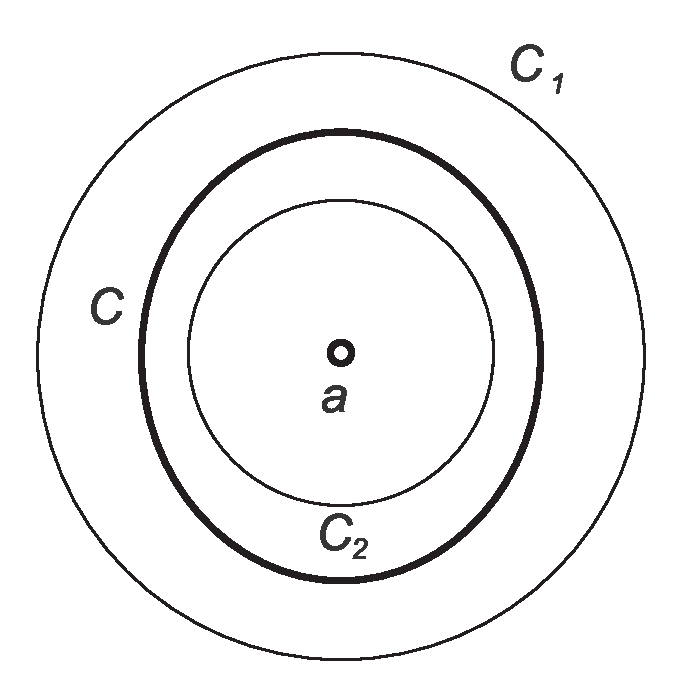
\includegraphics[width=0.35\textwidth]{fig-344.eps}
\caption{Teorema de Laurent}
\label{fig-344}
\end{figure}

Como no caso da s\'{e}rie de Taylor, $f$ pode ser singular em
alguns pontos no exterior de $\mathcal{C}_1$ e constituindo uma
caracter\'{\i}stica nova essencial $f(z)$ pode ser singular em alguns
pontos no interior de $\mathcal{C}_2$.

\begin{theoc}{Teorema de Laurent}{} Se $f$ for anal\'{\i}tica e un\'{\i}voca
sobre duas circunfer\^{e}ncias conc\^{e}ntricas $\mathcal{C}_1$, e
$\mathcal{C}_2$ com centro em $a$ e na coroa por elas limitada,
ent\~{a}o $f$ pode ser representada pela s\'{e}rie de Laurent
\begin{align}
  f(z) & =\sum_{n\geq 0}b_n(z-a)^n+\sum_{n\geq 1}\frac{c_n}{(z-a)^n}\nonumber\\[2ex]
   & =b_0+b_1(z-a)+b_2(z-a)^2+\cdots+\frac{c_1}{z-a}+\frac{c_2}{(z-a)^2}+\cdots\label{laure145:1}
\end{align}
onde
\begin{equation}\label{laure145:2}
b_n= \frac{1}{2\pi j}\int_{\mathcal{C}}\frac{f(w)}{(w -
a)^{n+1}}dw,\qquad  c_n=\frac{1}{2\pi j}\int_{\mathcal{C}}(w -
a)^{n-1}f(w)dw
\end{equation}
\end{theoc}
cada integral sendo calculada no sentido direto em torno de
qualquer caminho fechado simples $\mathcal{C}$, que se situa na
coroa e envolve a circunfer\^{e}ncia menor ver Figura~\ref{fig-344}.

Esta s\'{e}rie converge e representa $f(z)$ na coroa aberta que se
obt\'{e}m da coroa dada aumetando continuamente a circunfer\^{e}ncia
$\mathcal{C}_1$ e diminuindo $\mathcal{C}_2$ at\'{e} que cada uma
delas atinja um ponto onde $f$ seja singular.


\begin{obs} Evidentemente, em lugar de \eqref{laure145:1} e \eqref{laure145:2} podemos escrever
simplesmente
\begin{equation}\label{laure145:3}
f(z)=\sum_{n\in \mathbb{Z}}A_n(z-a)^n
\end{equation}
onde
\begin{equation}\label{laure145:4}
A_n=\frac{1}{2\pi j}\int_{\mathcal{C}}\frac{f(w)}{(w - a)^{n+1}}dw
\end{equation}
\end{obs}

\prova \textbf{do Teorema de Laurent.} Seja $z$ qualquer ponto na
coroa dada. Ent\~{a}o, de acordo com a f\'{o}rmula integral de Cauchy no
caso de um dom\'{\i}nio de conex\~{a}o m\'{u}ltipla segue-se que
\begin{equation}\label{laure145:5}
 f(z)=\frac{1}{2\pi j}\int_{\mathcal{C}_1}\frac{f(w)}{w -
z}dw-\frac{1}{2\pi j}\int_{\mathcal{C}_2}\frac{f(w)}{w - z}dw
\end{equation}
onde ambas as integrais s\~{a}o calculadas no sentido direto. Estas
integrais ser\~{a}o agora transformadas de uma maneira semelhante \`{a}
empregada no desenvolvimento de Taylor. Como $z$ se situa no
interior de $\mathcal{C}_1$ a primeira destas integrais \'{e}
precisamente do mesmo tipo que a integral \eqref{tay141:1}.
Desenvolvendo e estimando o resto, obtemos
\begin{equation}\label{laure145:6}
\frac{1}{2\pi j}\int_{\mathcal{C}_1}\frac{f(w)}{w -
z}dw=\sum_{n\geq 0}b_n(z-a)^n
\end{equation}
onde os coeficientes s\~{a}o dados pela f\'{o}rmula
\begin{equation}\label{laure145:7}
b_n=\frac{1}{2\pi j}\int_{\mathcal{C}_1}\frac{f(w)}{(w -
z)^{n+1}}dw,
\end{equation}
representamos a vari\'{a}vel de integra\c{c}\~{a}o por $w$, j\'{a} que $z$ \'{e}
empregada em $f(z)$, e a integral \'{e} tomada no sentido direto. Como
a n\~{a}o \'{e} um ponto da coroa, as fun\c{c}\~{o}es $f(w)/(w - a)^{n+1}$ s\~{a}o
anal\'{\i}ticas na coroa. Assim, podemos integrar ao longo do caminho
$\mathcal{C}$, em lugar de $\mathcal{C}_1$ sem alterar o valor de
$b_n$.\; Isto demonstra \eqref{laure145:2} para todo $n\geq 0$.

No caso da \'{u}ltima integral, a situa\c{c}\~{a}o \'{e} diferente j\'{a} que $z$ se
situa no exterior de $\mathcal{C}_2$. Em lugar de
\eqref{tay141:3}, temos que
\begin{equation}\label{laure145:8}
 \left|\frac{w - a}{z - a}\right| < 1
\end{equation}
isto \'{e}, temos que desenvolver $1/(w - z)$ em pot\^{e}ncias de $(w -
a)/(z - a)$ para a s\'{e}rie resultante ser convergente. Obtemos
\begin{equation*}
\frac{1}{w- z}= \frac{1}{w - a - (z - a)}= \frac{-1}{(z - a)
\left(1- \frac{w - z}{z - a}\right)}
\end{equation*}

Aplicando a f\'{o}rmula para uma progress\~{a}o geom\'{e}trica finita \`{a} \'{u}ltima
express\~{a}o ela se toma
\begin{align*}
\frac{1}{w - a}&=- \frac{1}{z- a}\left\{1+\frac{w-a}{z-a} +
\left(\frac{w - a}{z- a}\right)^2+\cdots+\left(\frac{w -
a}{z-a}\right)^n\right\}\\[2ex]
&\quad-\frac{1}{z-w}\left(\frac{w - a}{z-a}\right)^{n+1}
\end{align*}

Deste desenvolvimento prontamente obtemos
\begin{align*}
- \frac{1}{2\pi j}&\int_{\mathcal{C}_2}\frac{f(w)}{w -
z}dw \\[2ex]
   &=\frac{1}{2\pi
   j}\left\{\frac{1}{z-a}\int_{\mathcal{C}_2}f(w)dw+\frac{1}{(z-a)^2}
   \int_{\mathcal{C}_2}(w
   -a)f(w)dw+\cdots\right.\\[2ex]
   &\left.+ \frac{1}{(z-a)^{n+1}}\int_{\mathcal{C}_2}(w -
a)^{n}f(w)dw\right\}+R^*_n(z);
\end{align*}
nesta representa\c{c}\~{a}o o \'{u}ltimo termo \'{e} da forma
\begin{equation}\label{laure145:9}
 R_n(z)= \frac{1}{2\pi j(z - a)^{n+1}}\int_{\mathcal{C}_2} \frac{(w -a)^{n+1}}{z-w}
 f(w)dw
\end{equation}

Nas integrais do segundo membro podemos substituir a
circunfer\^{e}ncia $\mathcal{C}_2$ pelo anteriormente mencionado
caminho $\mathcal{C}$, sem alterar seus valores. Assim, o teorema
de Laurent fica demonstrado se provarmos que
\begin{equation}\label{laure145:10}
 \lim_{n\to\infty} R_n(z) = 0.
\end{equation}

Demonstremos \eqref{laure145:10}. Como $z - w \neq 0$ e $f$ \'{e}
anal\'{\i}tica na coroa e sobre $\mathcal{C}_2$, o valor absoluto da
express\~{a}o $f(w)/(z - w)$ \'{e} limitado, digamos
\begin{equation*}
\left|\frac{f(w)}{z - w}\right| < \tilde{M},\quad \text{para
qualquer } \quad w \in \mathcal{C}_2.
\end{equation*}

Aplicando estimativa de valor absoluto a uma integral de linha \`{a}
\eqref{laure145:9}, e representando o comprimento de
$\mathcal{C}_2$ por $l$, obtemos
\begin{equation*}
|R_n^*(z)| < \frac{1}{2\pi|z-a|^{n+1}} |w - a|^{n+1}\tilde{M}l =
\frac{\tilde{M} l}{2\pi} \left|\frac{w - a}{z - a}\right|^{n+1}
\end{equation*}

De \eqref{laure145:8} conclu\'{\i}mos que a express\~{a}o da direita se
aproxima de zero \`{a} medida que $n$ se aproxima do infinito. Assim,
\eqref{laure145:10} fica demonstrada. A representa\c{c}\~{a}o
\eqref{laure145:1} com coeficientes \eqref{laure145:2} fica
estabelecida na coroa dada.

Finalmente, vamos demonstrar a converg\^{e}ncia de \eqref{laure145:1}
na coroa aberta caracterizada no fim do teorema.

Representamos as somas das duas s\'{e}ries em \eqref{laure145:1} por
$g(z)$ e $h(z)$ e os raios de $\mathcal{C}_1$ e $\mathcal{C}_2$
por $r_1$ e $r_2$ respectivamente. Assim, $f = g + h$. A primeira
s\'{e}rie \'{e} uma s\'{e}rie de pot\^{e}ncias. De vez que ela converge na coroa,
ela deve convergir em todo o disco limitado por $\mathcal{C}_1$ e
$g$ \'{e} anal\'{\i}tica no disco.

Fazendo $Z = 1/(z - a)$, a \'{u}ltima s\'{e}rie se transforma numa s\'{e}rie
de pot\^{e}ncias em $Z$. A coroa $r_2 <| z - a | < r_1$, ent\~{a}o
corresponde \`{a} coroa $1/r_1 < | Z| < 1/r_2$, a nova s\'{e}rie converge
na coroa e, portanto, em todo o disco $| Z | < 1/r_2$. Agora, como
o disco corresponde a $|z- a| > r_2$, o exterior de
$\mathcal{C}_2$, a s\'{e}rie dada converge para todo $z$ no exterior
de $\mathcal{C}_2$ e $h$ \'{e} anal\'{\i}tica para todos estes valores de
$z$.

Como $f = g + h$, segue-se que $g$ deve ser singular em todos
aqueles pontos no exterior de $\mathcal{C}_2$, onde $f$ \'{e}
singular, e $h$ deve ser singular em todos aqueles pontos no
interior de $\mathcal{C}_2$ onde $f$ \'{e} singular. Conseq\"{u}entemente,
o raio de converg\^{e}ncia da primeira s\'{e}rie \'{e} igual \`{a} dist\^{a}ncia da
singularidade de $f$, no exterior de $\mathcal{C}_1$ que \'{e} mais
pr\'{o}xima de $a$. Semelhantemente, a segunda s\'{e}rie converge para
todo $z$ no exterior de uma circunfer\^{e}ncia com centro em a cujo
raio \'{e} igual \`{a} dist\^{a}ncia m\'{a}xima das singularidades de $f$ no
interior de $\mathcal{C}_2$.

O dom\'{\i}nio comum a ambos estes dom\'{\i}nios \'{e} a coroa aberta caracterizada
no fim do teorema; assim a demonstra\c{c}\~{a}o fica completa.

Segue-se que, se $f$ for anal\'{\i}tica no interior de
$\mathcal{C}_2$, a s\'{e}rie de Laurent se reduz \`{a} s\'{e}rie de Taylor de
$f$ com centro em $a$. Realmente, aplicando o teorema integral
de Cauchy a \eqref{laure145:2}, vemos que, neste caso, todos os
coeficientes das pot\^{e}ncias negativas em \eqref{laure145:1} s\~{a}o
zero.

Al\'{e}m disso, se $z = a$ for o \'{u}nico ponto singular de $f$ em
$\mathcal{C}_2$, ent\~{a}o o desenvolvimento de Laurent
\eqref{laure145:1} converge para todo $z$ em $\mathcal{C}_1$
exceto em $z = a$. Este caso ocorre freq\"{u}entemente e possui,
portanto, particular import\^{a}ncia.

A s\'{e}rie de Laurent de uma dada fun\c{c}\~{a}o anal\'{\i}tica $f$ em sua
coroa de converg\^{e}ncia \'{e} \'{u}nica (veja os exerc\'{\i}cios desta se\c{c}\~{a}o).
Entretanto, $f$ pode possuir s\'{e}ries de Laurent diferentes em
duas coroas com o mesmo centro (veja  Exemplo~\ref{xe145:2},
abaixo).

A unicidade \'{e} importante, porque a s\'{e}rie de Laurent em geral n\~{a}o \'{e}
obtida empregando \eqref{laure145:2} para calcular os
coeficientes, mas por v\'{a}rios outros m\'{e}todos. Alguns destes m\'{e}todos
s\~{a}o ilustrados nos exemplos que se seguem. Se uma s\'{e}rie de Laurent
for determinada por um destes processos, ela deve ser a s\'{e}rie de
Laurent da fun\c{c}\~{a}o dada na coroa fixada. \qed

\begin{exer}\label{xe145:1}
Obtenha a s\'{e}rie de Laurent de $z^2e^{1/z}$ com centro em $0$.
\end{exer}

 \solo Pode ser obtida de \eqref{elem142:2}. Substituindo $z$ por $1/z$ naquela
s\'{e}rie vem
\begin{align*}
  z^2e^{1/z} &=z^2\left( 1+\frac{1}{1!z}+\frac{1}{2!z^2}+\cdots \right) \\[2ex]
   &=z^2  + z + \frac{1}{2} + \frac{1}{3!z}+\frac{1}{4!z}+\cdots,  \qquad|z| >0.
\end{align*}

Assim obtemos a s\'{e}rie de Laurent.\hfill \(\lozenge\)

\begin{exer}\label{xe145:2}
Determinar todas as s\'{e}ries de Laurent de $f(z) =
1/(1-z^2)$ com centro em $z = 1$.
\end{exer}

\solo  Temos $1 - z^2= -(z - 1) (z + 1)$. Empregando a s\'{e}rie
geom\'{e}trica
\begin{equation*}
 \frac{1}{1-q} =\sum_{n\geq 0}q^n\qquad |q|<1,
\end{equation*}
empregamos
\begin{align}
  \frac{1}{z+1} &= \frac{1}{2+(z-1)}=\frac{1}{2}\frac{1}{\left[1-\left(-\frac{z-1}{2}
  \right)\right]}\nonumber\\[2ex]
   &= \frac{1}{2}\sum_{n\geq 0}\left(-\frac{z-1}{2} \right)^n=\sum_{n\geq 0}
   \frac{(-1)^{n+1}}{2^{n+1}}(z-1)^n\label{laure145:a}
\end{align}

esta s\'{e}rie converge no disco $|(z - 1)/2| < 1$, isto \'{e}, $|z-1| <
2$. Semelhantemente,
\begin{align}
\frac{1}{z+1} &=
\frac{1}{(z-1)+2}=\frac{1}{z-1}\frac{1}{\left[1+\left(\frac{2}{z-1}\right)\right]}
\nonumber\\[2ex]
&= \frac{1}{z-1}\sum_{n\geq 0}\left(-\frac{2}{z-1} \right)^n=\sum_{n\geq 0}
   \frac{(-2)^{n}}{(z-1)^{n+1}}\label{laure145:b}
\end{align}

esta s\'{e}rie converge para $|2/(z - 1)| < 1$, isto \'{e}, $|z - 1|>2$.
Portanto, de \eqref{laure145:a} obtemos
\begin{align*}
f(z) &=\frac{-1}{(z-1)(z+1)}=\sum_{n\geq 0}\frac{(-1)^{n+1}}{2^{n+1}}(z-1)^{n-1}\\[2ex]
   &=\frac{-1/2}{z-1}+\frac{1}{4}-\frac{1}{8}(z-1)+\frac{1}{16}(z-1)^2-+\cdots;
\end{align*}

esta s\'{e}rie converge no dom\'{\i}nio $0 < | z - 1| < 2$. De
\eqref{laure145:b}
\begin{equation*}
f(z) =-\sum_{n\geq
0}\frac{(-2)^{n}}{(z-1)^{n+2}}=-\frac{1}{(z-1)^2}+\frac{2}{(z-1)^3}-
\frac{4}{(z-1)^4}+-\cdots,
\quad |z-1|>2
\end{equation*}

Portanto existem varias s\'{e}ries de Laurent.\hfill \(\lozenge\)

\begin{exer}\label{xe145:3}
Utilizando o exerc\'{\i}cio do fim da se\c{c}\~{a}o s\'{e}ries de Taylor das
fun\c{c}\~{o}es elementares, obtenha a s\'{e}rie de Laurent da fun\c{c}\~{a}o $\cot
z$.
\end{exer}

\solo Com efeito,
\begin{equation*}
\cot(z)
=\frac{1}{z}-\frac{1}{3}z-\frac{1}{45}z^3-\frac{2}{945}z^5-\cdots,\quad
0<|z|<\pi.
\end{equation*}

Obtendo a s\'{e}rie pedida. \hfill \(\lozenge\)

%%%
\section*{Exerc\'{\i}cios Propostos} 
%%%
Resolver os seguintes exerc\'{\i}cios sobre fun\c{c}\~{o}es complexas
\begin{enumerate}[label=(\arabic*)]
\item Desenvolver as seguintes fun\c{c}\~{o}es em s\'{e}ries de Laurent;
convergentes para a desigualdade $0 <| z |<R$ e determinar
precisamente a regi\~{a}o de converg\^{e}ncia.
\begin{tasks}[](2)
\rm{(a)}&\quad \frac{e^{-z}}{z^3}
\rm{(b)}&\quad \frac{e^{1/z^2}}{z^6}
\rm{(c)}&\quad \frac{\cos(2z)}{z^2}
\rm{(d)}&\quad \frac{1}{z^4(1+z)}
\rm{(e)}&\quad \frac{1}{z^2(1-z^2)}
\rm{(f)}&\quad \frac{1}{z^2(z-3)}
\rm{(g)}&\quad \frac{\senh(3z)}{z^3}
\rm{(h)}&\quad \frac{1}{z^4+z^8}
\end{tasks}

\item Demonstrar que o desenvolvimento de Laurent de uma dada fun\c{c}\~{a}o
anal\'{\i}tica em uma dada coroa \'{e} \'{u}nico.

\item Determinar todas as s\'{e}ries de Taylor e de Laurent com centro
em $z = a$ e determinar precisamente as regi\~{o}es de converg\^{e}ncia:
\begin{tasks}[](2)
\rm{(a)}&\quad \dfrac{1}{z^2+1}, \quad  a=-j 
\rm{(b)}&\quad \dfrac{1}{z^4}, \quad a=1
\rm{(c)}&\quad \dfrac{1}{z^3}, \quad a=j 
\rm{(d)}&\quad \dfrac{7z^2+9z-18}{z^3-9z},quad  a=0
\rm{(e)}&\quad \dfrac{4z^2+2z-4}{z^3-4z},\quad a=2 
\rm{(f)}&\quad \dfrac{\sen(z)}{(z-\pi/4)},\quad a=\pi /4
\end{tasks}
\end{enumerate}

%%%%%
\section{Comportamento de Fun\c{c}\~{o}es no Infinito}
%%%%
Veremos na pr\'{o}xima se\c{c}\~{a}o que a s\'{e}rie de Laurent pode ser empregada
para classificar as singularidades das fun\c{c}\~{o}es anal\'{\i}ticas. Dentro
desta ordem de id\'{e}ias tamb\'{e}m consideraremos o comportamento das
fun\c{c}\~{o}es anal\'{\i}ticas $f$ quando $|z|$ se aproxima do infinito.

Para investigar o comportamento de uma fun\c{c}\~{a}o $f$ para $|z|$
grande, parece natural introduzir uma nova vari\'{a}vel $w$ fazendo
$z=1/w$ porque, ent\~{a}o, $|z|$ grande corresponde a $|w|$ pequeno, e
$|z|$ vai ao infinito  corresponde a $|w|$ vai ao zero.

A transforma\c{c}\~{a}o $w = 1/z$ foi considerada  no plano complexo
prolongado que foi obtido vinculando ao plano complexo finito, um
ponto impr\'{o}prio (o ponto no infinito). Podemos ent\~{a}o fazer $z
=\infty$ corresponder a $w = 0$ (e $w =\infty$ corresponder a $z =
0$). O procedimento de prolongar o plano complexo pode ser tamb\'{e}m
motivado pela considera\c{c}\~{a}o geom\'{e}trica simples que se segue.

A representa\c{c}\~{a}o usual dos n\'{u}meros complexos $\mathbb{C}$ no plano
complexo \'{e} conveniente enquanto os valores absolutos dos n\'{u}meros
n\~{a}o forem dema, siado grandes. Para $| z |$ grande a situa\c{c}\~{a}o se
toma inconveniente, e neste caso, podemos preferir uma
representa\c{c}\~{a}o dos n\'{u}meros complexos sobre uma esfera, a qual foi
sugerida por Riemann e se obt\'{e}m da seguinte maneira.

Seja $\mathcal{S}$ uma esfera de di\^{a}metro um que tangencia o plano
complexo $ \mathbb{C} $ na origem, ver Figura~\ref{fig-345}.
\begin{figure}[H]
\centering
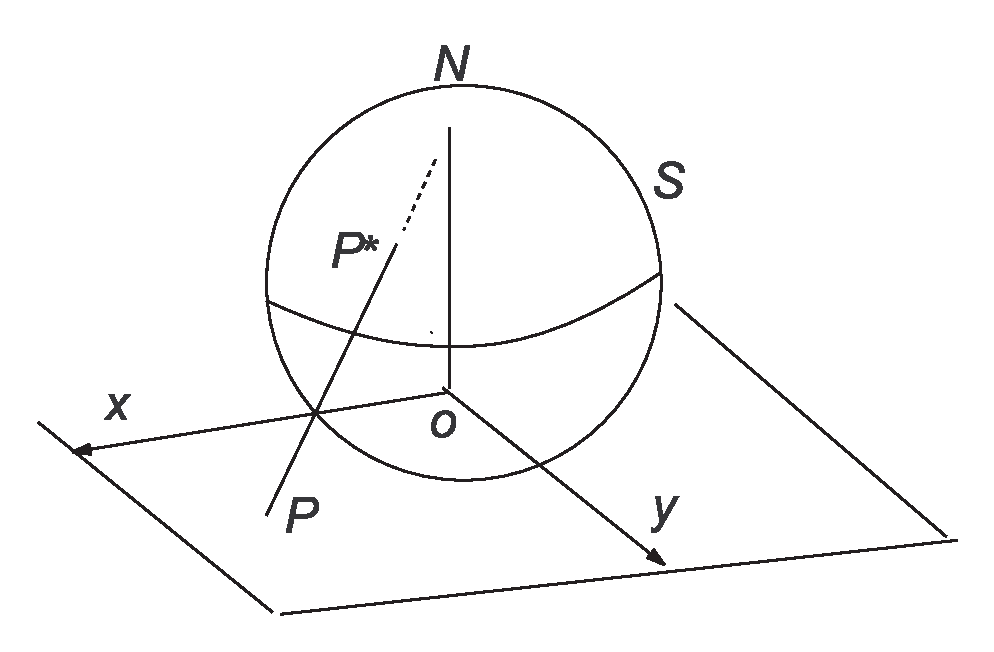
\includegraphics[width=0.5\textwidth]{fig-345.eps}
\caption{Esfera de Riemann} \label{fig-345}
\end{figure}

Seja $N$ o P\'{o}lo Norte de $\mathcal{S}$ (o ponto diametralmente
oposto ao ponto de contato entre a esfera e o plano). Seja $P$
qualquer ponto no plano complexo. Ent\~{a}o a reta definida por $P$ e
$N$ intercepta $\mathcal{S}$ no ponto $P^*$. Fazemos $P$ e $P^*$
corresponderem um ao outro. Desta maneira obtemos uma
correspond\'{e}ncia entre os pontos do plano complexo e os pontos
sobre $S$, e $P^*$ \'{e} a imagem do ponto $P$ nesta representa\c{c}\~{a}o. Os
n\'{u}meros complexos, primeiramente representados no plano, s\~{a}o
agora, representados por pontos sobre $\mathcal{S}$. A cada $z$
corresponde um ponto sobre $\mathcal{S}$. Reciprocamente, cada
ponto sobre $\mathcal{S}$ representa um n\'{u}mero complexo $z$,
exceto o ponto $N$ que n\~{a}o corresponde a nenhum ponto no plano
complexo.

Se, entretanto, introduzirmos o ponto impr\'{o}prio $z
=\infty$  e fizermos este ponto corresponder a $N$, a
representa\c{c}\~{a}o se transforma em uma representa\c{c}\~{a}o un\'{\i}voca do plano
prolongado sobre $\mathcal{S}$. A esfera $\mathcal{S}$ \'{e} chamada a
esfera dos n\'{u}meros de Riemann. A representa\c{c}\~{a}o particular que
empregamos \'{e} chamada uma proje\c{c}\~{a}o estereogr\'{a}fica.

Evidentemente, a circunfer\^{e}ncia unit\'{a}ria \'{e} representada sobre, o
``equador'' de $\mathcal{S}$. O interior da circunfer\^{e}ncia unit\'{a}ria
corresponde ao ``Hemisf\'{e}rio Sul" e o exterior ao ``Hemisf\'{e}rio
Norte'' Os n\'{u}meros $z$, cujos valores absolutos s\~{a}o grandes, se
situam pr\'{o}ximo ao P\'{o}lo Norte $N$. Os eixos dos $x$ e dos $y$ (e,
em geral, as retas que passam pela origem) s\~{a}o representadas sobre
os ``meridianos'', enquanto as circunfer\^{e}ncias com centro na origem
s\~{a}o representadas sobre os ``paralelos''.

Podemos demonstrar que qualquer circunfer\^{e}ncia ou reta no plano $\mathbb{C}$ \'{e}
representada sobre uma circunfer\^{e}ncia em $ \mathcal{S}$; al\'{e}m
disso, podemos provar que a \textit{proje\c{c}\~{a}o estereogr\'{a}fica} \'{e} conforme,
isto \'{e}, duas curvas quaisquer que se interceptam possuem imagens
cujo \^{a}ngulo de interse\c{c}\~{a}o \'{e} igual ao \^{a}ngulo de interse\c{c}\~{a}o das
curvas.

Dada uma fun\c{c}\~{a}o $f$ a ser investigada para $| z |$ grande,
podemos fazer $z =1/w$ e investigar $f(z) = f(1/w)\equiv g(w)$ em
uma vizinhan\c{c}a de $w = 0$. Definimos
\begin{equation*}
g(0) = \lim_{w\to 0} g(w),
\end{equation*}
e dizemos que $f(z)b$ \'{e} anal\'{\i}tica ou singular no infinito,
conforme $g(w)$ seja anal\'{\i}tica ou singular, respectivamente, em $w
= 0$.

\begin{exer}\label{infi146:1}
A fun\c{c}\~{a}o $f(z) = 1/z^2$ \'{e} anal\'{\i}tica no infinito, j\'{a} que $g(w) =
f(1/w)=w^2$ \'{e} anal\'{\i}tica em $w=0$. A fun\c{c}\~{a}o $f(z) = z^3$ \'{e} singular
no infinito porque $g(w) =f(1/w) = 1/w^2$ \'{e} singular em $w=0$. A
fun\c{c}\~{a}o exponencial $e^z$ \'{e} singular no infinito j\'{a} que $e^{1/w}$ \'{e}
singular em $w = 0$. Semelhantemente, as fun\c{c}\~{o}es trigonom\'{e}tricas
$\sen z$ e $\cos z$ s\~{a}o singulares no infinito.
\end{exer}

Seja $f(z)$ anal\'{\i}tica no exterior de uma circunfer\^{e}ncia
$\mathcal{C}$, digamos, no dom\'{\i}nio $|z - a| > R$, e tamb\'{e}m no
infinito. Se fizermos
\begin{equation*}
z= \frac{1}{w} + a,\quad \text{ ent\~{a}o }\quad z - a = \frac{1}{w}
\end{equation*}
e
\begin{equation*}
  f(z)=f\left(\frac{1}{w}+a \right)\equiv h(w)
\end{equation*}

\'{e} anal\'{\i}tica no disco $| w | < 1/R$. Seja a s\'{e}rie de Maclaurin de
$h(w)$
\begin{equation*}
h(w) =\sum_{n\geq 0}c_nw^n= c_o + c_1w + c_2w_2 + \cdots\qquad |w|
< \frac{1}{R}
\end{equation*}

Ent\~{a}o, substituindo $w = 1/(z - a)$ obtemos a s\'{e}rie de Laurent
\begin{equation}\label{infi146:2}
f(z) =\sum_{n\geq 0}\frac{c_n}{(z-a)^n}=c_o + \frac{c_1}{(z - a)}
+ \frac{c_2}{(z - a)^2}+\cdots,\quad |z-a|>R.
\end{equation}

Obtendo o que desejavamos.\hfill \(\lozenge\)

%%%
\section*{Exerc\'{\i}cios Propostos}
%%%% 
Resolver as quest\~{o}es a seguir sobre as fun\c{c}\~{o}es anal\'{\i}ticas
\begin{enumerate}[label=(\arabic*)]
\item As fun\c{c}\~{o}es seguintes s\~{a}o anal\'{\i}ticas no infinito ou n\~{a}o?
\begin{align*}
\rm{(a)}&\quad z^2 + z^{-2}   &\rm{(b)}&\quad  z^{-3}+z^{-1}\\[2ex]
\rm{(c)}&\quad e^z,\quad e^{z^2},\quad e^{-z} &\rm{(d)}& \quad e^{1/z},\quad e^{1/z^2}\\[2ex]
\rm{(e)}&\quad \cos(z),\quad \sen(z)  &\rm{(f)}&\quad \cosh(z),\quad\senh(z)\\[2ex]
\rm{(g)}&\quad ze^{1/z} &(h)&\quad 1/(z^2-3z)
\end{align*}

\item Descrever e esbo\c{c}ar as imagens das regi\~{o}es seguintes sobre a
esfera dos, n\'{u}meros de Riemann.
\begin{align*}
\rm{(a)}&\quad \textrm{Re}\; z\le 0  &\rm{(b)}&\quad \textrm{Im}\; z\geq 0\\[2ex]
\rm{(c)}&\quad  |z|\geq 5 &\rm{(d)}&\quad |z|\le 2\\[2ex]
\rm{(e)}&\quad 1/2\le |z|\le 2  &\rm{(f)}&\quad |z|\le 3,\quad |arg\; z|<\pi/2
\end{align*}

\item Empregando o m\'{e}todo descrito no fim desta se\c{c}\~{a}o, mostrar que
\begin{equation*}
\frac{1}{z^4}=\sum_{n\geq 0}{-4\choose n}(z-1)^{-n-4} =
\frac{1}{(z-1)^4}-\frac{4}{(z-1)^5}+\cdots,\qquad |z-1|>1
\end{equation*}
\end{enumerate}
